\documentclass[letterpaper,10pt]{book}
% Change to 10 pt
\usepackage{pdfpages}
\usepackage{morewrites}			% to counteract the no write space problem
\setcounter{tocdepth}{6}

\usepackage[framemethod=TikZ]{mdframed}

\usepackage{fancyhdr}

\usepackage{paralist}
\usepackage{amsmath}
\usepackage{amsfonts}
\usepackage{amssymb}
\usepackage{graphicx}

\usepackage{datetime}
%\usepackage{ulem}

%\usepackage[nottoc]{toobibind}

\usepackage[inline]{enumitem}

% Outer margin at 2.50 is exacty correct to fit the ``corruption alert'' tables
\usepackage[inner=1.0in, outer=2.50in, top=2.54cm,bottom=2.54cm, marginparwidth=2.25in]{geometry}

\usepackage{marginnote}
\usepackage{longtable}
\usepackage{booktabs}
\usepackage{xcolor}

\usepackage{soul}

%%%%%%%%%%%%
\definecolor{ForestGreen}{rgb}{0.00,0.29,0.098}
%%%%%%%%%%%%

\usepackage{marginnote}

\usepackage{imakeidx} 
\usepackage[
	backref=true,
	style=numeric,
%	citestyle=numeric,
	backend=bibtex
	]{biblatex}
\usepackage[driverfallback=hypertex,colorlinks=True]{hyperref}
\usepackage{cleveref}

\makeindex[name=scripture,columnsep=20pt, columnseprule=True,columns=3, title=Scripture References]
\makeindex[name=speaker,columnsep=20pt, columnseprule=True,,columns=2, title=Sermon Creator]
\makeindex[name=series,columnsep=20pt, columnseprule=True,,columns=2, title=Sermon Series]
\makeindex[name=date,columnsep=20pt, columnseprule=True,columns=2, title=Sermon Date]
\makeindex[name=event,columnsep=20pt, columnseprule=True,columns=2, title=Event]
\makeindex[name=topic,columnsep=20pt, columnseprule=True,columns=2, title=Topic]
\makeindex[name=AWIP,columnsep=20pt, columnseprule=True,columns=3, title=All Words in Passage]
\makeindex[name=NWIV,columnsep=20pt, columnseprule=True,columns=3, title=Number of Words in Verse]
\makeindex[name=PNIP,columnsep=20pt, columnseprule=True,columns=3, title=Proper Names in Passage]
\makeindex[name=PEIP,columnsep=20pt, columnseprule=True,columns=2, title=Prophetic Events in Passage]
\makeindex[name=TWPAQ,columnsep=20pt, columnseprule=True,columns=1, title=13-Word Phrases and Quotes]
\makeindex[name=PFTTIS,columnsep=20pt, columnseprule=False,columns=3, title=Phrases found 13 times in scripture]
\makeindex[name=WFTTIS,columnsep=20pt, columnseprule=False,columns=3, title=Words found 13 times in scripture]
\makeindex[name=WFITV,columnsep=20pt, columnseprule=False,columns=3, title=Words found in exactly 13 verses]
\makeindex[name=EVENTS,columnsep=20pt, columnseprule=False,columns=2, title=Sermon Log by Place]
\makeindex[name=QUESTIONS,columnsep=20pt, columnseprule=False,columns=2, title=Bible Questions]
\makeindex[name=DOCTRINES,columnsep=20pt, columnseprule=False,columns=2, title=Doctrines]
\makeindex[name=SONGS,columnsep=20pt, columnseprule=False,columns=1, title=Songs]
\makeindex[name=LOCATION,columnsep=20pt, columnseprule=False,columns= 2, title=Location]
\makeindex[name=FACEBOOK,columnsep=20pt, columnseprule=False,columns=2, title=Facebook]
\makeindex[name=DEVOTIONAL,columnsep=20pt, columnseprule=False,columns=2, title=Devotional Items]
%%%%%%%%%%%%%%%%% EXTRA COLORS
\definecolor{champagne}{rgb}{0.97,0.91,0.81}
\definecolor{bone}{rgb}{0.89,0.85,0.79}
\pagestyle{fancy}
\fancyhf{}
\fancyhead[LE,RO]{\today}
\fancyhead[RE,LO]{Daily Bible Reading}
\fancyhead[CE,CO]{-page \thepage  - }

\fancyfoot[CO,CE]{\leftmark}
%\fancyfoot[LE,RO]{CSCE 692, HW1}

\title{DBR\\
Daily \\ Reads}
\author{Keith Anthony \\
\today }
%+/ffffff +   \pagenumbering{gobble}
\bibliography{Bibliographies/All20220122}

\setlength{\fboxsep}{1.0pt}

\usepackage[utf8]{inputenc}
\usepackage{tikz}

\begin{document}
%%%%%%%%%%%% Tile Page

\begin{titlepage}

\begin{flushright}
\rightskip=-2.5cm
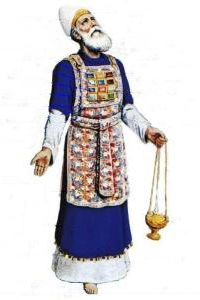
\includegraphics[width=50mm,scale=1.5]{Extras/Melchisedec.jpg}
\vspace{0.4in}  % Create a title for the document and write it in bold font
\LARGE{\textbf{\date}} % Again, do a line break
\linebreak 
% Create a subtitle \large{with Outlines, Statistics, Cross References, and Notes}
\vspace{0.5in}
\begin{flushleft}
\LARGE{Day \#75: Wednesday, 16  March 2022  \\}\vspace{0.25in}
\LARGE{Judges 7-9 Psalm 75 Proverb 16}
\end{flushleft}
\vspace{0.6in}
\bigskip

\normalsize{Xenia, Oh.\\}
\normalsize{created: \today}
\vspace{1.3in}

\end{flushright}
\end{titlepage}

\newpage 
\tableofcontents\hypertarget{TOC}{}
\listoffigures
\listoftables

\hyphenation{A-bim-e-lech bre-thren E-phra-im  Gib-e-o-nites Jer-u-sa-lem through-out Phil-i-stines The-o-phil-us Am-a-le-kites ven-geance Mesh-el-e-mi-ah onan-ism Phar-a-oh thoughts grev-ous-ness Hach-a-liah adul-ter-er Shad-rach}

%%%%%%%%%%%%%%%%% EXTRA COLORS
%%%%%%%%%%%%%%%%% EXTRA COLORS
%%%%%%%%%%%%%%%%% EXTRA COLORS
\definecolor{champagne}{rgb}{0.97,0.91,0.81}
\definecolor{bone}{rgb}{0.89,0.85,0.79}

\definecolor{ForestGreen}{rgb}{0.00,0.29,0.098}
\definecolor{GIVING}{cmyk}{1,0.0,0.72,.1}

\definecolor{MLPE}{cmyk}{1,1,0,.45}
\definecolor{SOCCER}{cmyk}{.77, 0, .42, .49}
\definecolor{PAYBILL}{cmyk}{0,0.83,0.76,0.07}
\definecolor{SERMON}{cmyk}{.14,.9,0,.30} % aka seance \href{http://www.flatuicolorpicker.com/purple-cmyk-color-model/}{seance}
\definecolor{BIBLE}{cmyk}{0,.17,.74,.17}
\definecolor{WORKBLUE}{cmyk}{1, .5, 0, .6}
\definecolor{myOrange}{cmyk}{0, .4, .98, .03}
\definecolor{myTan}{cmyk}{0.0,.07,.17,.10}
\definecolor{myRed}{cmyk}{0,1,1,0}
\definecolor{myWhite}{cmyk}{0,0,0,0}
\definecolor{BLUESoD}{cmyk}{.97,.84,0,.04}
\definecolor{WHITE}{cmyk}{0,0,0,0}
\definecolor{OLDGOLD}{cmyk}{0.05,0.3,1.00,0}
\definecolor{CASTLETON}{cmyk}{1,0,0.31,0.66}
\definecolor{cadmiumgreen}{rgb}{0.0, 0.42, 0.24}
\definecolor{jungle}{rgb}{0.203,0.4882,0.1718}
\definecolor{MYGOLD}{rgb}{1,.84,0}

\definecolor{MYLIGHTGRAY}{rgb}{.85,.85,.85}

\definecolor{codegreen}{rgb}{0,0.6,0}
\definecolor{codegray}{rgb}{0.5,0.5,0.5}
\definecolor{codepurple}{rgb}{0.58,0,0.82}
\definecolor{backcolour}{rgb}{0.95,0.95,0.92}


\mdfdefinestyle{MyFrame}{%
    linecolor=blue,
    outerlinewidth=2pt,
    roundcorner=5pt,
    innertopmargin=\baselineskip,
    innerbottommargin=\baselineskip,
    innerrightmargin=10pt,
    innerleftmargin=10pt,
    backgroundcolor=gray!25!white}


\mdfdefinestyle{MyFrame2}{%
    linecolor=black,
    outerlinewidth=2pt,
    roundcorner=5pt,
    innertopmargin=\baselineskip,
    innerbottommargin=\baselineskip,
    innerrightmargin=10pt,
    innerleftmargin=10pt,
    backgroundcolor=yellow!25!white}


%%%%%
%% for PFTTIS list
%%%%%

%%% And Joseph said unto
\index[PFTTIS]{And Joseph said unto!Genesis!Gen 40:008}
\index[PFTTIS]{And Joseph said unto!Genesis!Gen 40:012}
\index[PFTTIS]{And Joseph said unto!Genesis!Gen 41:025}
\index[PFTTIS]{And Joseph said unto!Genesis!Gen 42:014}
\index[PFTTIS]{And Joseph said unto!Genesis!Gen 42:018}
\index[PFTTIS]{And Joseph said unto!Genesis!Gen 44:015}
\index[PFTTIS]{And Joseph said unto!Genesis!Gen 45:003}
\index[PFTTIS]{And Joseph said unto!Genesis!Gen 45:004}
\index[PFTTIS]{And Joseph said unto!Genesis!Gen 46:031}
\index[PFTTIS]{And Joseph said unto!Genesis!Gen 48:009}
\index[PFTTIS]{And Joseph said unto!Genesis!Gen 48:018}
\index[PFTTIS]{And Joseph said unto!Genesis!Gen 50:019}
\index[PFTTIS]{And Joseph said unto!Genesis!Gen 50:024}


%%% a shadow
\index[PFTTIS]{a shadow!1Chronicles!1Chr 029:15}
\index[PFTTIS]{a shadow!Job!Job 008:09}
\index[PFTTIS]{a shadow!Job!Job 014:02}
\index[PFTTIS]{a shadow!Job!Job 017:07}
\index[PFTTIS]{a shadow!Psalm!Psa 102:011}
\index[PFTTIS]{a shadow!Psalm!Psa 144:004}
\index[PFTTIS]{a shadow!Ecclesiastes!Eccl 006:012}
\index[PFTTIS]{a shadow!Ecclesiastes!Eccl 008:013}
\index[PFTTIS]{a shadow!Isaiah!Isa 04:006}
\index[PFTTIS]{a shadow!Isaiah!Isa 25:004}
\index[PFTTIS]{a shadow!Jonah!Jnh 04:06}
\index[PFTTIS]{a shadow!Colossians!Col 02:017}
\index[PFTTIS]{a shadow!Hebews!Heb 10:001}

%%% blessed is the man
\index[PFTTIS]{blessed is the man!Psalm!Psa 001:001}
\index[PFTTIS]{blessed is the man!Psalm!Psa 032:002}
\index[PFTTIS]{blessed is the man!Psalm!Psa 034:008}
\index[PFTTIS]{blessed is the man!Psalm!Psa 065:004}
\index[PFTTIS]{blessed is the man!Psalm!Psa 084:005}
\index[PFTTIS]{blessed is the man!Psalm!Psa 084:012}
\index[PFTTIS]{blessed is the man!Psalm!Psa 094:012}
\index[PFTTIS]{blessed is the man!Psalm!Psa 112:001}
\index[PFTTIS]{blessed is the man!Proverbs!Pro 008:034}
\index[PFTTIS]{blessed is the man!Isaiah!Isa 056:002}
\index[PFTTIS]{blessed is the man!Jeremiah!Jer 017:007}
\index[PFTTIS]{blessed is the man!Romans!Rom 004:008}
\index[PFTTIS]{blessed is the man!James!Jam 001:012}


%%% carry them
\index[PFTTIS]{carry them!Leviticus!Lev 14:045}
\index[PFTTIS]{carry them!Numbers!Num 11:012}
\index[PFTTIS]{carry them!Joshua!Jsh 04:003}
\index[PFTTIS]{carry them!1Samuel!1Sam 20:040}
\index[PFTTIS]{carry them!1Kings!1Kng 08:046}
\index[PFTTIS]{carry them!2Chronicles!2Chr 06:036}
\index[PFTTIS]{carry them!Ezra!Ezra 05:015}
\index[PFTTIS]{carry them!Isaiah!Isa 40:011}
\index[PFTTIS]{carry them!Isaiah!Isa 41:016}
\index[PFTTIS]{carry them!Isaiah!Isa 57:013}
\index[PFTTIS]{carry them!Jeremiah!Jer 20:004}
\index[PFTTIS]{carry them!Jeremiah!Jer 20:005}
\index[PFTTIS]{carry them!Jeremiah!Jer 43:012}


\index[PFTTIS]{good tidings!2Samuel!2Sam 18:027}
\index[PFTTIS]{good tidings!1Kings!1Ki 01:042}
\index[PFTTIS]{good tidings!2Kings!2Ki 07:009 (2x)}
\index[PFTTIS]{good tidings!Isaiah!Isa 40:009 (2x)}
\index[PFTTIS]{good tidings!Isaiah!Isa 41:007}
\index[PFTTIS]{good tidings!Isaiah!Isa 52:007}
\index[PFTTIS]{good tidings!Isaiah!Isa 61:001}
\index[PFTTIS]{good tidings!Nahum!Nah 01:005}
\index[PFTTIS]{good tidings!Luke!Lk 02:010}
\index[PFTTIS]{good tidings!1Thessalonians!1Thess 03:006}


%%% dead body
\index[PFTTIS]{dead body!Leviticus!Lev 21:011}
\index[PFTTIS]{dead body!Numbers!Num 06:006}
\index[PFTTIS]{dead body!Numbers!Num 09:006}
\index[PFTTIS]{dead body!Numbers!Num 09:007}
\index[PFTTIS]{dead body!Numbers!Num 09:010}
\index[PFTTIS]{dead body!Numbers!Num 09:011}
\index[PFTTIS]{dead body!Numbers!Num 09:013}
\index[PFTTIS]{dead body!Numbers!Num 09:016}
\index[PFTTIS]{dead body!2Kings!2Ki 08:005}
\index[PFTTIS]{dead body!Isaiah!Isa 26:019}
\index[PFTTIS]{dead body!Jeremiah!Jer 26:023}
\index[PFTTIS]{dead body!Jeremiah!Jer 36:030}
\index[PFTTIS]{dead body!Haggai!Hag 02:013}

%%% great sea
\index[PFTTIS]{great sea!Numbers!Num 34:006}
\index[PFTTIS]{great sea!Numbers!Num 34:007}
\index[PFTTIS]{great sea!Joshua!Jos 01:004}
\index[PFTTIS]{great sea!Joshua!Jos 09:001}
\index[PFTTIS]{great sea!Joshua!Jos 15:012}
\index[PFTTIS]{great sea!Joshua!Jos 15:047}
\index[PFTTIS]{great sea!Joshua!Jos 23:004}
\index[PFTTIS]{great sea!Ezekiel!Eze 47:010}
\index[PFTTIS]{great sea!Ezekiel!Eze 47:015}
\index[PFTTIS]{great sea!Ezekiel!Eze 47:019}
\index[PFTTIS]{great sea!Ezekiel!Eze 47:020}
\index[PFTTIS]{great sea!Ezekiel!Eze 48:028}
\index[PFTTIS]{great sea!Daniel!Dan 07:002}


%%% have forsaken me
\index[PFTTIS]{have forsaken me!Judges!Jdg 10:013}
\index[PFTTIS]{have forsaken me!1Samuel!1Sam 08:008}
\index[PFTTIS]{have forsaken me!1Kings!1Ki 11:033}
\index[PFTTIS]{have forsaken me!2Kings!2Ki 22:017}
\index[PFTTIS]{have forsaken me!2Chronicles!2Chr 12:005}
\index[PFTTIS]{have forsaken me!2Chronicles!2Chr 34:025}
\index[PFTTIS]{have forsaken me!Jeremiah!Jer 01:016}
\index[PFTTIS]{have forsaken me!Jeremiah!Jer 02:013}
\index[PFTTIS]{have forsaken me!Jeremiah!Jer 05:007}
\index[PFTTIS]{have forsaken me!Jeremiah!Jer 05:019}
\index[PFTTIS]{have forsaken me!Jeremiah!Jer 16:011 (2x)}
\index[PFTTIS]{have forsaken me!Jeremiah!Jer 19:004}

%%% no king
\index[PFTTIS]{no king!Judges!Jdg 17:06}
\index[PFTTIS]{no king!Judges!Jdg 18:01}
\index[PFTTIS]{no king!Judges!Jdg 19:01}
\index[PFTTIS]{no king!Judges!Jdg 21:25}
\index[PFTTIS]{no king!1Kings!1Ki 22:47}
\index[PFTTIS]{no king!2Kings!2Ki 23:25}
\index[PFTTIS]{no king!Nehemiah!Neh 13:26}
\index[PFTTIS]{no king!Psalms!Psa 033:016}
\index[PFTTIS]{no king!Proverbs!Pro 30:27}
\index[PFTTIS]{no king!Daniel!Dan 02:10}
\index[PFTTIS]{no king!Hosea!Hos 10:03}
\index[PFTTIS]{no king!Micah!Mic 04:09}
\index[PFTTIS]{no king!John!Jhn 19:15}


%%% rebellious house
\index[PFTTIS]{rebellious house!Exodus!Exo 02:005}
\index[PFTTIS]{rebellious house!Exodus!Exo 02:006}
\index[PFTTIS]{rebellious house!Exodus!Exo 02:008}
\index[PFTTIS]{rebellious house!Exodus!Exo 03:009}
\index[PFTTIS]{rebellious house!Exodus!Exo 03:026}
\index[PFTTIS]{rebellious house!Exodus!Exo 03:027}
\index[PFTTIS]{rebellious house!Exodus!Exo 12:002 (2x)}
\index[PFTTIS]{rebellious house!Exodus!Exo 12:003}
\index[PFTTIS]{rebellious house!Exodus!Exo 12:009}
\index[PFTTIS]{rebellious house!Exodus!Exo 12:025}
\index[PFTTIS]{rebellious house!Exodus!Exo 17:012}
\index[PFTTIS]{rebellious house!Exodus!Exo 24:003}

%%% seek him
\index[PFTTIS]{seek him!Deuteronomy!Deu 04:029}\index[PFTTIS]{seek him!1Samuel!1Sam 23:025}
\index[PFTTIS]{seek him!1Chronicles!1Chr 28:009}
\index[PFTTIS]{seek him!2Chronicles!1Chr 15:002}
\index[PFTTIS]{seek him!Ezra!Ezr 08:022}
\index[PFTTIS]{seek him!Psalms!Psa 022:026}
\index[PFTTIS]{seek him!Psalms!Psa 024:006}
\index[PFTTIS]{seek him!Psalms!Psa 119:002}
\index[PFTTIS]{seek him!SoS!SoS 03:002}
\index[PFTTIS]{seek him!SoS!SoS 06:001}
\index[PFTTIS]{seek him!Hosea!Hos 07:010}
\index[PFTTIS]{seek him!Amos!Amo 05:008}
\index[PFTTIS]{seek him!Hebrews!Heb 11:0063}


%%% seek ye
\index[PFTTIS]{seek ye!Isaiah!Isa 34:016}
\index[PFTTIS]{seek ye!Isaiah!Isa 45:019}
\index[PFTTIS]{seek ye!Isaiah!Isa 55:006}
\index[PFTTIS]{seek ye!Amos!Amos 5:004}
\index[PFTTIS]{seek ye!John!John 1:38}
\index[PFTTIS]{seek ye!John!John 18:4}
\index[PFTTIS]{seek ye!John!John 18:7}
\index[PFTTIS]{seek ye!Matthew!Matt 6:33}
\index[PFTTIS]{seek ye!Numbers!Num 16:10}
\index[PFTTIS]{seek ye!Luke!Luke 12:31}
\index[PFTTIS]{seek ye!Luke!Luke 24:5}
\index[PFTTIS]{seek ye!Psalm!Psa 27:8}
\index[PFTTIS]{seek ye!Zephaniah!Zeph 2:3}

%%% the uncircumcised
\index[PFTTIS]{the uncircumcised!Genesis!Gen 17:014}
\index[PFTTIS]{the uncircumcised!Judges!Jdg 14:003}
\index[PFTTIS]{the uncircumcised!Judges!Jdg 15:018}
\index[PFTTIS]{the uncircumcised!2Samuel!2Sam 01:020}
\index[PFTTIS]{the uncircumcised!Isaiah!Isa 02:001}
\index[PFTTIS]{the uncircumcised!Jeremiah!Jer 09:025}
\index[PFTTIS]{the uncircumcised!Ezekiel!Eze 28:010}
\index[PFTTIS]{the uncircumcised!Ezekiel!Eze 31:018}
\index[PFTTIS]{the uncircumcised!Ezekiel!Eze 32:019}
\index[PFTTIS]{the uncircumcised!Ezekiel!Eze 32:027}
\index[PFTTIS]{the uncircumcised!Ezekiel!Eze 32:028}
\index[PFTTIS]{the uncircumcised!Ezekiel!Eze 32:029}
\index[PFTTIS]{the uncircumcised!Ezekiel!Eze 32:032}

%%% worship him
\index[PFTTIS]{worship him!Psalms!Psa 97:007}
\index[PFTTIS]{worship him!Zephaniah!Zeph 02:011}
\index[PFTTIS]{worship him!Matthew!Matt 02:002}
\index[PFTTIS]{worship him!Matthew!Matt 02:008}
\index[PFTTIS]{worship him!John!John 04:023}
\index[PFTTIS]{worship him!John!John 04:024 (2x)} 
\index[PFTTIS]{worship him!Acts!Acts 17:023}
\index[PFTTIS]{worship him!Hebrews!Heb 01:006}
\index[PFTTIS]{worship him!Revelation!Rev 04:010}
\index[PFTTIS]{worship him!Revelation!Rev 13:008}
\index[PFTTIS]{worship him!Revelation!Rev 14:007}
\index[PFTTIS]{worship him!Revelation!Rev 19:010}


%%%%%
%% for PFTTIS list
%%%%%

%%% afflictions
\index[WFTTIS]{afflictions!Psalms!Psa 34:019}
\index[WFTTIS]{afflictions!Psalms!Psa 132:001}
\index[WFTTIS]{afflictions!Acts!Acts 07:010}
\index[WFTTIS]{afflictions!Acts!Acts 20:023}
\index[WFTTIS]{afflictions!2Corinthians!2Cor 06:004}
\index[WFTTIS]{afflictions!Colossians!Col 01:024}
\index[WFTTIS]{afflictions!1Thessalonians!1Thess 03:003}
\index[WFTTIS]{afflictions!2Timothy!2Tim 01:008}
\index[WFTTIS]{afflictions!2Timothy!2Tim 03:011}
\index[WFTTIS]{afflictions!2Timothy!2Tim 04:005}
\index[WFTTIS]{afflictions!Hebrews!Heb 10:032}
\index[WFTTIS]{afflictions!Hebrews!Heb 10:033}
\index[WFTTIS]{afflictions!1Peter!1Pet 05:009}

%%% acsend
\index[WFTTIS]{acsend!Joshua!Jos 06:05}
\index[WFTTIS]{acsend!Psalm!Psa 024:003}
\index[WFTTIS]{acsend!Psalm!Psa 135:007}
\index[WFTTIS]{acsend!Psalm!Psa 139:008}
\index[WFTTIS]{acsend!Isaiah!Isa 14:013}
\index[WFTTIS]{acsend!Isaiah!Isa 14:014}
\index[WFTTIS]{acsend!Jeremiah!Jer 10:013}
\index[WFTTIS]{acsend!Jeremiah!Jer 51:016}
\index[WFTTIS]{acsend!Ezekiel!Eze 38:009}
\index[WFTTIS]{acsend!John!John 06:062}
\index[WFTTIS]{acsend!John!John 20:017}
\index[WFTTIS]{acsend!Romans!Rom 10:006}
\index[WFTTIS]{acsend!Revelation!Rev 17:008}

%%% Assyrian
\index[WFTTIS]{Assyrian!Isaiah!Isa 10:005}
\index[WFTTIS]{Assyrian!Isaiah!Isa 10:024}
\index[WFTTIS]{Assyrian!Isaiah!Isa 14:025}
\index[WFTTIS]{Assyrian!Isaiah!Isa 19:023}
\index[WFTTIS]{Assyrian!Isaiah!Isa 23:013}
\index[WFTTIS]{Assyrian!Isaiah!Isa 30:031}
\index[WFTTIS]{Assyrian!Isaiah!Isa 31:008}
\index[WFTTIS]{Assyrian!Isaiah!Isa 52:004}
\index[WFTTIS]{Assyrian!Ezekiel!Eze 31:003}
\index[WFTTIS]{Assyrian!Hosea!Hos 05:013}
\index[WFTTIS]{Assyrian!Hosea!Hos 11:005}
\index[WFTTIS]{Assyrian!Micah!Hos 05:005}
\index[WFTTIS]{Assyrian!Micah!Hos 05:006}

%%% blot
\index[WFTTIS]{blot!Exodus!Exo 32:032}
\index[WFTTIS]{blot!Exodus!Exo 32:033}
\index[WFTTIS]{blot!Numbers!Num 05:026}
\index[WFTTIS]{blot!Deuteronomy!Deut 09:014}
\index[WFTTIS]{blot!Deuteronomy!Deut 25:019}
\index[WFTTIS]{blot!Deuteronomy!Deut 29:020}
\index[WFTTIS]{blot!2Kings!2Ki 14:027}
\index[WFTTIS]{blot!Job!Job 31:007}
\index[WFTTIS]{blot!Psalms!Psa 51:001}
\index[WFTTIS]{blot!Psalms!Psa 51:009}
\index[WFTTIS]{blot!Proverbs!Pro 09:007}
\index[WFTTIS]{blot!Jeremiah!Jer 18:023}
\index[WFTTIS]{blot!Revelation!Rev 03:005}


%%% chain
\index[WFTTIS]{chain!Genesis!Gen 41:042}
\index[WFTTIS]{chain!1Kings!1Ki 07:017}
\index[WFTTIS]{chain!Psalms!Psa 73:006}
\index[WFTTIS]{chain!SoS!Sos 04:009}
\index[WFTTIS]{chain!Lamentations!Lam 03:007}
\index[WFTTIS]{chain!Ezekiel!Eze 07:023}
\index[WFTTIS]{chain!Ezekiel!Eze 16:011}
\index[WFTTIS]{chain!Daniel!Dan 05:007}
\index[WFTTIS]{chain!Daniel!Dan 05:016}
\index[WFTTIS]{chain!Daniel!Dan 05:029}
\index[WFTTIS]{chain!Acts!Acts 28:020}
\index[WFTTIS]{chain!2Timothy!2Tim 01:016}
\index[WFTTIS]{chain!Revelation!Rev 20:001}


%%% controversy
\index[WFTTIS]{controversy!Deuteronomy!Deu 17:008}
\index[WFTTIS]{controversy!Deuteronomy!Deu 19:017}
\index[WFTTIS]{controversy!Deuteronomy!Deu 21:005}
\index[WFTTIS]{controversy!Deuteronomy!Deu 25:001}
\index[WFTTIS]{controversy!2Samuel!2Sam 15:002}
\index[WFTTIS]{controversy!Isaiah!Isa 34:008}
\index[WFTTIS]{controversy!Jeremiah!Jer 25:031}
\index[WFTTIS]{controversy!Ezekiel!Eze 44:024}
\index[WFTTIS]{controversy!Hosea!Hos 04:001}
\index[WFTTIS]{controversy!Hosea!Hos 12:002}
\index[WFTTIS]{controversy!Micah!Mic 06:002 (2x)}
\index[WFTTIS]{controversy!1Timothy!1Tim 03:016}


%%% Dagon/Dagon's
\index[WFTTIS]{Dagon!Judges!Jdg 16:023}
\index[WFTTIS]{Dagon!1Samuel!1Sam 05:002 (2x)}
\index[WFTTIS]{Dagon!1Samuel!1Sam 05:003 (2x)}
\index[WFTTIS]{Dagon!1Samuel!1Sam 05:004 (3x)}
\index[WFTTIS]{Dagon!1Samuel!1Sam 05:005 (3x)}
\index[WFTTIS]{Dagon!1Samuel!1Sam 05:007}
\index[WFTTIS]{Dagon!1Chronicles!1Chr 10:010}

%%% disobedient
\index[WFTTIS]{disobedient!1Kings!1Ki 13:026}
\index[WFTTIS]{disobedient!Nehemiah!Neh 09:026}
\index[WFTTIS]{disobedient!Luke!Luke 01:017}
\index[WFTTIS]{disobedient!Acts!Acts 26:019}
\index[WFTTIS]{disobedient!Romans!Rom 01:030}
\index[WFTTIS]{disobedient!Romans!Rom 10:021}
\index[WFTTIS]{disobedient!1Timothy!1Tim 01:009}
\index[WFTTIS]{disobedient!2Timothy!2Tim 03:002}
\index[WFTTIS]{disobedient!Titus!Titus 01:016}
\index[WFTTIS]{disobedient!Titus!Titus 03:003}
\index[WFTTIS]{disobedient!1Peter!1Pet 02:007}
\index[WFTTIS]{disobedient!1Peter!1Pet 02:008}
\index[WFTTIS]{disobedient!1Peter!1Pet 03:020}


%%% doubt
\index[WFTTIS]{doubt!Genesis!Gen 37:033}
\index[WFTTIS]{doubt!Deuteronomy!Deu 28:066}
\index[WFTTIS]{doubt!Job!Job 12:002}
\index[WFTTIS]{doubt!Matthew!Matt 14:031}
\index[WFTTIS]{doubt!Matthew!Matt 21:021}
\index[WFTTIS]{doubt!Mark!Mk 11:023}
\index[WFTTIS]{doubt!Luke!Lk 11:020}
\index[WFTTIS]{doubt!John!Jhn 10:024}
\index[WFTTIS]{doubt!Acts!Acts 02:012}
\index[WFTTIS]{doubt!Acts!Acts 28:004}
\index[WFTTIS]{doubt!1Corinthians!1Cor 09:010}
\index[WFTTIS]{doubt!Galatians!Gal 04:020}
\index[WFTTIS]{doubt!1John!1Jhn 02:019}


%%% dungeon
\index[WFTTIS]{dungeon!Genesis!Gen 40:015}
\index[WFTTIS]{dungeon!Genesis!Gen 41:014}
\index[WFTTIS]{dungeon!Exodus!Exo 12:029}
\index[WFTTIS]{dungeon!Jeremiah!Jer 37:016}
\index[WFTTIS]{dungeon!Jeremiah!Jer 38:006 (2x)}
\index[WFTTIS]{dungeon!Jeremiah!Jer 38:007}
\index[WFTTIS]{dungeon!Jeremiah!Jer 38:009}
\index[WFTTIS]{dungeon!Jeremiah!Jer 38:010}
\index[WFTTIS]{dungeon!Jeremiah!Jer 38:011}
\index[WFTTIS]{dungeon!Jeremiah!Jer 38:013}
\index[WFTTIS]{dungeon!Lamentations!Lam 03:053}
\index[WFTTIS]{dungeon!Lamentations!Lam 03:055}


%%% error
\index[WFTTIS]{error!2Samuel!2Sam 06:007}
\index[WFTTIS]{error!Job!Job 19:004}
\index[WFTTIS]{error!Ecclesiastes!Ecc 05:006}
\index[WFTTIS]{error!Ecclesiastes!Ecc 10:005}
\index[WFTTIS]{error!Isaiah!Isa 32:006}
\index[WFTTIS]{error!Daniel!Dan 06:004}
\index[WFTTIS]{error!Matthew!Matt 27:064}
\index[WFTTIS]{error!Romans!Rom 01:027}
\index[WFTTIS]{error!James!Jam 05:020}
\index[WFTTIS]{error!2Peter!2Pet 02:018}
\index[WFTTIS]{error!2Peter!2Pet 03:017}
\index[WFTTIS]{error!1John!1Jn 04:006}
\index[WFTTIS]{error!Jude!Jude 01:011}

%%% fourish
\index[WFTTIS]{fourish!Psalms!Psa 072:007}
\index[WFTTIS]{fourish!Psalms!Psa 072:016}
\index[WFTTIS]{fourish!Psalms!Psa 092:007}
\index[WFTTIS]{fourish!Psalms!Psa 092:012}
\index[WFTTIS]{fourish!Psalms!Psa 092:013}
\index[WFTTIS]{fourish!Psalms!Psa 132:018}
\index[WFTTIS]{fourish!Proverbs!Pro 11:28}
\index[WFTTIS]{fourish!Proverbs!Pro 14:11}
\index[WFTTIS]{fourish!Ecclesiastes!Ecc 12:05}
\index[WFTTIS]{fourish!SongOfSolomon!SOS 07:12}
\index[WFTTIS]{fourish!Isaiah!Isa 17:11}
\index[WFTTIS]{fourish!Isaiah!Isa 66:14}
\index[WFTTIS]{fourish!Ezekiel!Eze 17:24}




%%% giants
\index[WFTTIS]{giants!Genesis!Gen 06:004}
\index[WFTTIS]{giants!Numbers!Num 13:033}
\index[WFTTIS]{giants!Deuteronomy!Deut 02:011}
\index[WFTTIS]{giants!Deuteronomy!Deut 02:021}
\index[WFTTIS]{giants!Deuteronomy!Deut 03:011}
\index[WFTTIS]{giants!Deuteronomy!Deut 03:013}
\index[WFTTIS]{giants!Joshua!Josh 12:004}
\index[WFTTIS]{giants!Joshua!Josh 13:012}
\index[WFTTIS]{giants!Joshua!Josh 15:008}
\index[WFTTIS]{giants!Joshua!Josh 17:015}
\index[WFTTIS]{giants!Joshua!Josh 16:016}

%%% good man
\index[WFTTIS]{good man!2 Samuel!2Sa 18:27}
%(1) Psalms 37:23 [5]
%(1) Psalms 112:5 [2]
%(1) Proverbs 12:2 [2]
%(1) Proverbs 13:22 [2]
%(1) Proverbs 14:14 [14]
%(1) Micah 7:2 [2]
%(1) Matthew 12:35 [2]
%(1) Luke 6:45 [2]
%(1) Luke 23:50 [15]
%(1) John 7:12 [17]
%(1) Acts 11:24 [5]
%(1) Romans 5:7 [14]

%%% Hinnom
\index[WFTTIS]{Hinnom!Joshua!Jsh 15:008}
\index[WFTTIS]{Hinnom!Joshua!Jsh 18:016}
\index[WFTTIS]{Hinnom!2Kings!2Ki 23:010}
\index[WFTTIS]{Hinnom!2Chronicles!2Chr 28:003}
\index[WFTTIS]{Hinnom!2Chronicles!2Chr 33:006}
\index[WFTTIS]{Hinnom!Nehemiah!Neh 11:030}
\index[WFTTIS]{Hinnom!Jeremiah!Jer 07:031}
\index[WFTTIS]{Hinnom!Jeremiah!Jer 07:032}
\index[WFTTIS]{Hinnom!Jeremiah!Jer 19:002}
\index[WFTTIS]{Hinnom!Jeremiah!Jer 19:006}
\index[WFTTIS]{Hinnom!Jeremiah!Jer 32:035}

%%% inclined
\index[WFTTIS]{inclined!Judges!Jdg 09:003}
\index[WFTTIS]{inclined!Psalms!Psa 040:001}
\index[WFTTIS]{inclined!Psalms!Psa 116:002}
\index[WFTTIS]{inclined!Psalms!Psa 119:112}
\index[WFTTIS]{inclined!Proverbs!Pro 05:13}
\index[WFTTIS]{inclined!Jeremiah!Jer 07:24}
\index[WFTTIS]{inclined!Jeremiah!Jer 07:26}
\index[WFTTIS]{inclined!Jeremiah!Jer 11:08}
\index[WFTTIS]{inclined!Jeremiah!Jer 17:23}
\index[WFTTIS]{inclined!Jeremiah!Jer 25:04}
\index[WFTTIS]{inclined!Jeremiah!Jer 34:14}
\index[WFTTIS]{inclined!Jeremiah!Jer 35:15}
\index[WFTTIS]{inclined!Jeremiah!Jer 44:05}


%%% laughed
\index[WFTTIS]{laughed!Genesis!Gen 17:017}
\index[WFTTIS]{laughed!Genesis!Gen 18:012}
\index[WFTTIS]{laughed!Genesis!Gen 18:015}
\index[WFTTIS]{laughed!2Kings!2Ki 19:021}
\index[WFTTIS]{laughed!2Chronicles!2Chr 30:010}
\index[WFTTIS]{laughed!Nehemiah!Neh 02:019}
\index[WFTTIS]{laughed!Job!Job 12:004}
\index[WFTTIS]{laughed!Job!Job 29:024}
\index[WFTTIS]{laughed!Isaiah!Isa 37:022}
\index[WFTTIS]{laughed!Ezekiel!Ezek 23:032}
\index[WFTTIS]{laughed!Matthew!Matt 09:024}
\index[WFTTIS]{laughed!Mark!Mk 05:040}
\index[WFTTIS]{laughed!Luke!Lk 08:053}

%%% liar
\index[WFTTIS]{liar!Job!Job 24:025}
\index[WFTTIS]{liar!Proverbs!Pro 17:004}
\index[WFTTIS]{liar!Proverbs!Pro 19:022}
\index[WFTTIS]{liar!Proverbs!Pro 30:006}
\index[WFTTIS]{liar!Jeremiah!Jer 15:018}
\index[WFTTIS]{liar!John!Jhn 08:044}
\index[WFTTIS]{liar!John!Jhn 08:055}
\index[WFTTIS]{liar!Romans!Rom 03:004}
\index[WFTTIS]{liar!1John!1Jhn 01:010}
\index[WFTTIS]{liar!1John!1Jhn 02:004}
\index[WFTTIS]{liar!1John!1Jhn 02:022}
\index[WFTTIS]{liar!1John!1Jhn 04:020}
\index[WFTTIS]{liar!1John!1Jhn 05:010}

%%% palsy
\index[WFTTIS]{palsy!Matthew!Matt 04:024}
\index[WFTTIS]{palsy!Matthew!Matt 08:006}
\index[WFTTIS]{palsy!Matthew!Matt 09:002}
\index[WFTTIS]{palsy!Matthew!Matt 09:006}
\index[WFTTIS]{palsy!Mark!Mk 02:003}
\index[WFTTIS]{palsy!Mark!Mk 02:004}
\index[WFTTIS]{palsy!Mark!Mk 02:005}
\index[WFTTIS]{palsy!Mark!Mk 02:009}
\index[WFTTIS]{palsy!Mark!Mk 02:010}
\index[WFTTIS]{palsy!Luke!Lk 05:018}
\index[WFTTIS]{palsy!Luke!Lk 05:024}
\index[WFTTIS]{palsy!Acts!Acts 09:033}

%%% Profitable
\index[WFTTIS]{profitable!Job!Job 22:002 (2x)}
\index[WFTTIS]{profitable!Ecclesiastes!Ecc 10:010}
\index[WFTTIS]{profitable!Isaiah!Isa 44:010}
\index[WFTTIS]{profitable!Jeremiah!Jer 13:007}
\index[WFTTIS]{profitable!Matthew!Matt 05:029}
\index[WFTTIS]{profitable!Matthew!Matt 05:030}
\index[WFTTIS]{profitable!Acts!Acts 20:020}
\index[WFTTIS]{profitable!1Timothy!1Tim 04:008}
\index[WFTTIS]{profitable!2Timothy!2Tim 03:016}
\index[WFTTIS]{profitable!2Timothy!2Tim 04:011}
\index[WFTTIS]{profitable!Titus!Titus 03:008}
\index[WFTTIS]{profitable!Philemon!Phlm 01:011}

%%% Rechab
\index[WFTTIS]{Rechab!2Samuel!2Sam 04:002}
\index[WFTTIS]{Rechab!2Samuel!2Sam 04:005}
\index[WFTTIS]{Rechab!2Samuel!2Sam 04:006}
\index[WFTTIS]{Rechab!2Samuel!2Sam 04:009}
\index[WFTTIS]{Rechab!2KIngs!2Ki 10:015}
\index[WFTTIS]{Rechab!2KIngs!2Ki 10:023}
\index[WFTTIS]{Rechab!1Chronicles!1Chr 02:055}
\index[WFTTIS]{Rechab!Nehemiah!Neh 03:014}
\index[WFTTIS]{Rechab!Jeremiah!Jer 35:006}
\index[WFTTIS]{Rechab!Jeremiah!Jer 35:008}
\index[WFTTIS]{Rechab!Jeremiah!Jer 35:014}
\index[WFTTIS]{Rechab!Jeremiah!Jer 35:016}
\index[WFTTIS]{Rechab!Jeremiah!Jer 35:019}

%%% serpents
\index[WFTTIS]{serpents!Exodus!Exo 07:012}
\index[WFTTIS]{serpents!Numbers!Num 21:006}
\index[WFTTIS]{serpents!Numbers!Num 21:007}
\index[WFTTIS]{serpents!Deuteronomy!Deu 08:015}
\index[WFTTIS]{serpents!Deuteronomy!Deu 32:024}
\index[WFTTIS]{serpents!Jeremiah!Jer 08:017}
\index[WFTTIS]{serpents!Matthew!Matt 10:016}
\index[WFTTIS]{serpents!Matthew!Matt 23:033}
\index[WFTTIS]{serpents!Mark!Mk 16:018}
\index[WFTTIS]{serpents!Luke!Lk 10:019}
\index[WFTTIS]{serpents!1Corinthians!1Cor 10:009}
\index[WFTTIS]{serpents!James!Jas 03:007}
\index[WFTTIS]{serpents!Revelation!Rev 09:019}

%%% short
\index[WFTTIS]{short!Numbers!Num 11:023}
\index[WFTTIS]{short!2Kings!2Ki 10:032}
\index[WFTTIS]{short!Job!Job 17:012}
\index[WFTTIS]{short!Job!Job 20:005}
\index[WFTTIS]{short!Psalms!Psa 89:047}
\index[WFTTIS]{short!Romans!Rom 03:023}
\index[WFTTIS]{short!Romans!Rom 09:028  (2x)}
\index[WFTTIS]{short!1Corinthians!1Cor 07:029}
\index[WFTTIS]{short!1Thessalonians!1Thess 02:017}
\index[WFTTIS]{short!Hebrews!Heb 04:001}
\index[WFTTIS]{short!Revelation!Rev 12:012}
\index[WFTTIS]{short!Revelation!Rev 17:010}

%%% smiteth
\index[WFTTIS]{smiteth!Exodus!Exo 21:012}
\index[WFTTIS]{smiteth!Exodus!Exo 21:15}
\index[WFTTIS]{smiteth!Deuteronomy!Dt 25:11}
\index[WFTTIS]{smiteth!Deuteronomy!Dt 27:24}
\index[WFTTIS]{smiteth!Joshua!Jsh 15:16}
\index[WFTTIS]{smiteth!Judges!Jdg 15:16}
\index[WFTTIS]{smiteth!2 Samuel!2Sa 05:08}
\index[WFTTIS]{smiteth!1Chronicles!1Chr 11:06}
\index[WFTTIS]{smiteth!Job!1Chr 26:12}
\index[WFTTIS]{smiteth!Isaiah!Isa 09:13}
\index[WFTTIS]{smiteth!Lamentations!Lam 03:30}
\index[WFTTIS]{smiteth!Ezekiel!Eze 07:09}
\index[WFTTIS]{smiteth!Luke!Lk 06:29}



%%% vanities
\index[WFTTIS]{vanities!Deuteronomy!Deut 21:021}
\index[WFTTIS]{vanities!1Kings!1Ki 16:013}
\index[WFTTIS]{vanities!1Kings!1Ki 16:026}
\index[WFTTIS]{vanities!Psalms!Psa 031:006}
\index[WFTTIS]{vanities!Ecclesiastes!Ecc 01:002 (2x)}
\index[WFTTIS]{vanities!Ecclesiastes!Ecc 05:007}
\index[WFTTIS]{vanities!Ecclesiastes!Ecc 12:008}
\index[WFTTIS]{vanities!Jeremiah!Jer 08:019}
\index[WFTTIS]{vanities!Jeremiah!Jer 10:008}
\index[WFTTIS]{vanities!Jeremiah!Jer 14:022}
\index[WFTTIS]{vanities!Jonah!Jnh 02:008}
\index[WFTTIS]{vanities!Acts!Acts 14:015}



%%%%%
%% for PFTTIS list
%%%%%

%%% worm
\index[WFITV]{worm!Exodus!Exo 16:024}
\index[WFITV]{worm!Job!Job 17:014}
\index[WFITV]{worm!Job!Job 24:029}
\index[WFITV]{worm!Job!Job 25:005 (2x)}
\index[WFITV]{worm!Psalms!Psa 022:006}
\index[WFITV]{worm!Isaiah!Isa 14:011}
\index[WFITV]{worm!Isaiah!Isa 41:014}
\index[WFITV]{worm!Isaiah!Isa 51:008}
\index[WFITV]{worm!Isaiah!Isa 66:024}
\index[WFITV]{worm!Jonah!Jnh 04:007}
\index[WFITV]{worm!Mark!Mk 09:044}
\index[WFITV]{worm!Mark!Mk 09:046}
\index[WFITV]{worm!Mark!Mk 09:048}


%\subsubsection{Title}
%\textbf{Introduction:} Isaiah 46 
%\index[speaker]{Speaker!Isaiah 49 (Title}
%\index[series]{Book (Speaker)!IPassage (Title)}
%\index[date]{2017/07/09!Isaiah 49 (Title)}
%\begin{compactenum}[I.]
%    \item  \textbf{Point} \index[scripture]{Isaiah!IPassage} (IPassage)
%\end{compactenum}




  


%\input{02OT-Exodus/ExodusIntroduction}

%\newpage
%\begin{figure}
%\begin{center}
%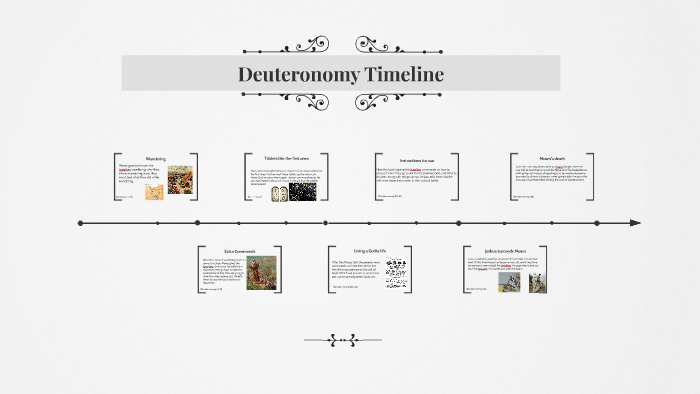
\includegraphics[scale=.7, angle=0]{05OT-Deuteronomy/References/AndrewSmithDeuteronomyTimeline.png}
%\caption[Deuteronomy Timeline by Andrew Smith]{Deuteronomy Timeline by Andrew %Smith}
%\label{fig:Deuteronomy Timeline by Andrew Smith}
%\end{center}
%\end{figure}

\newpage
\begin{figure}
\begin{center}
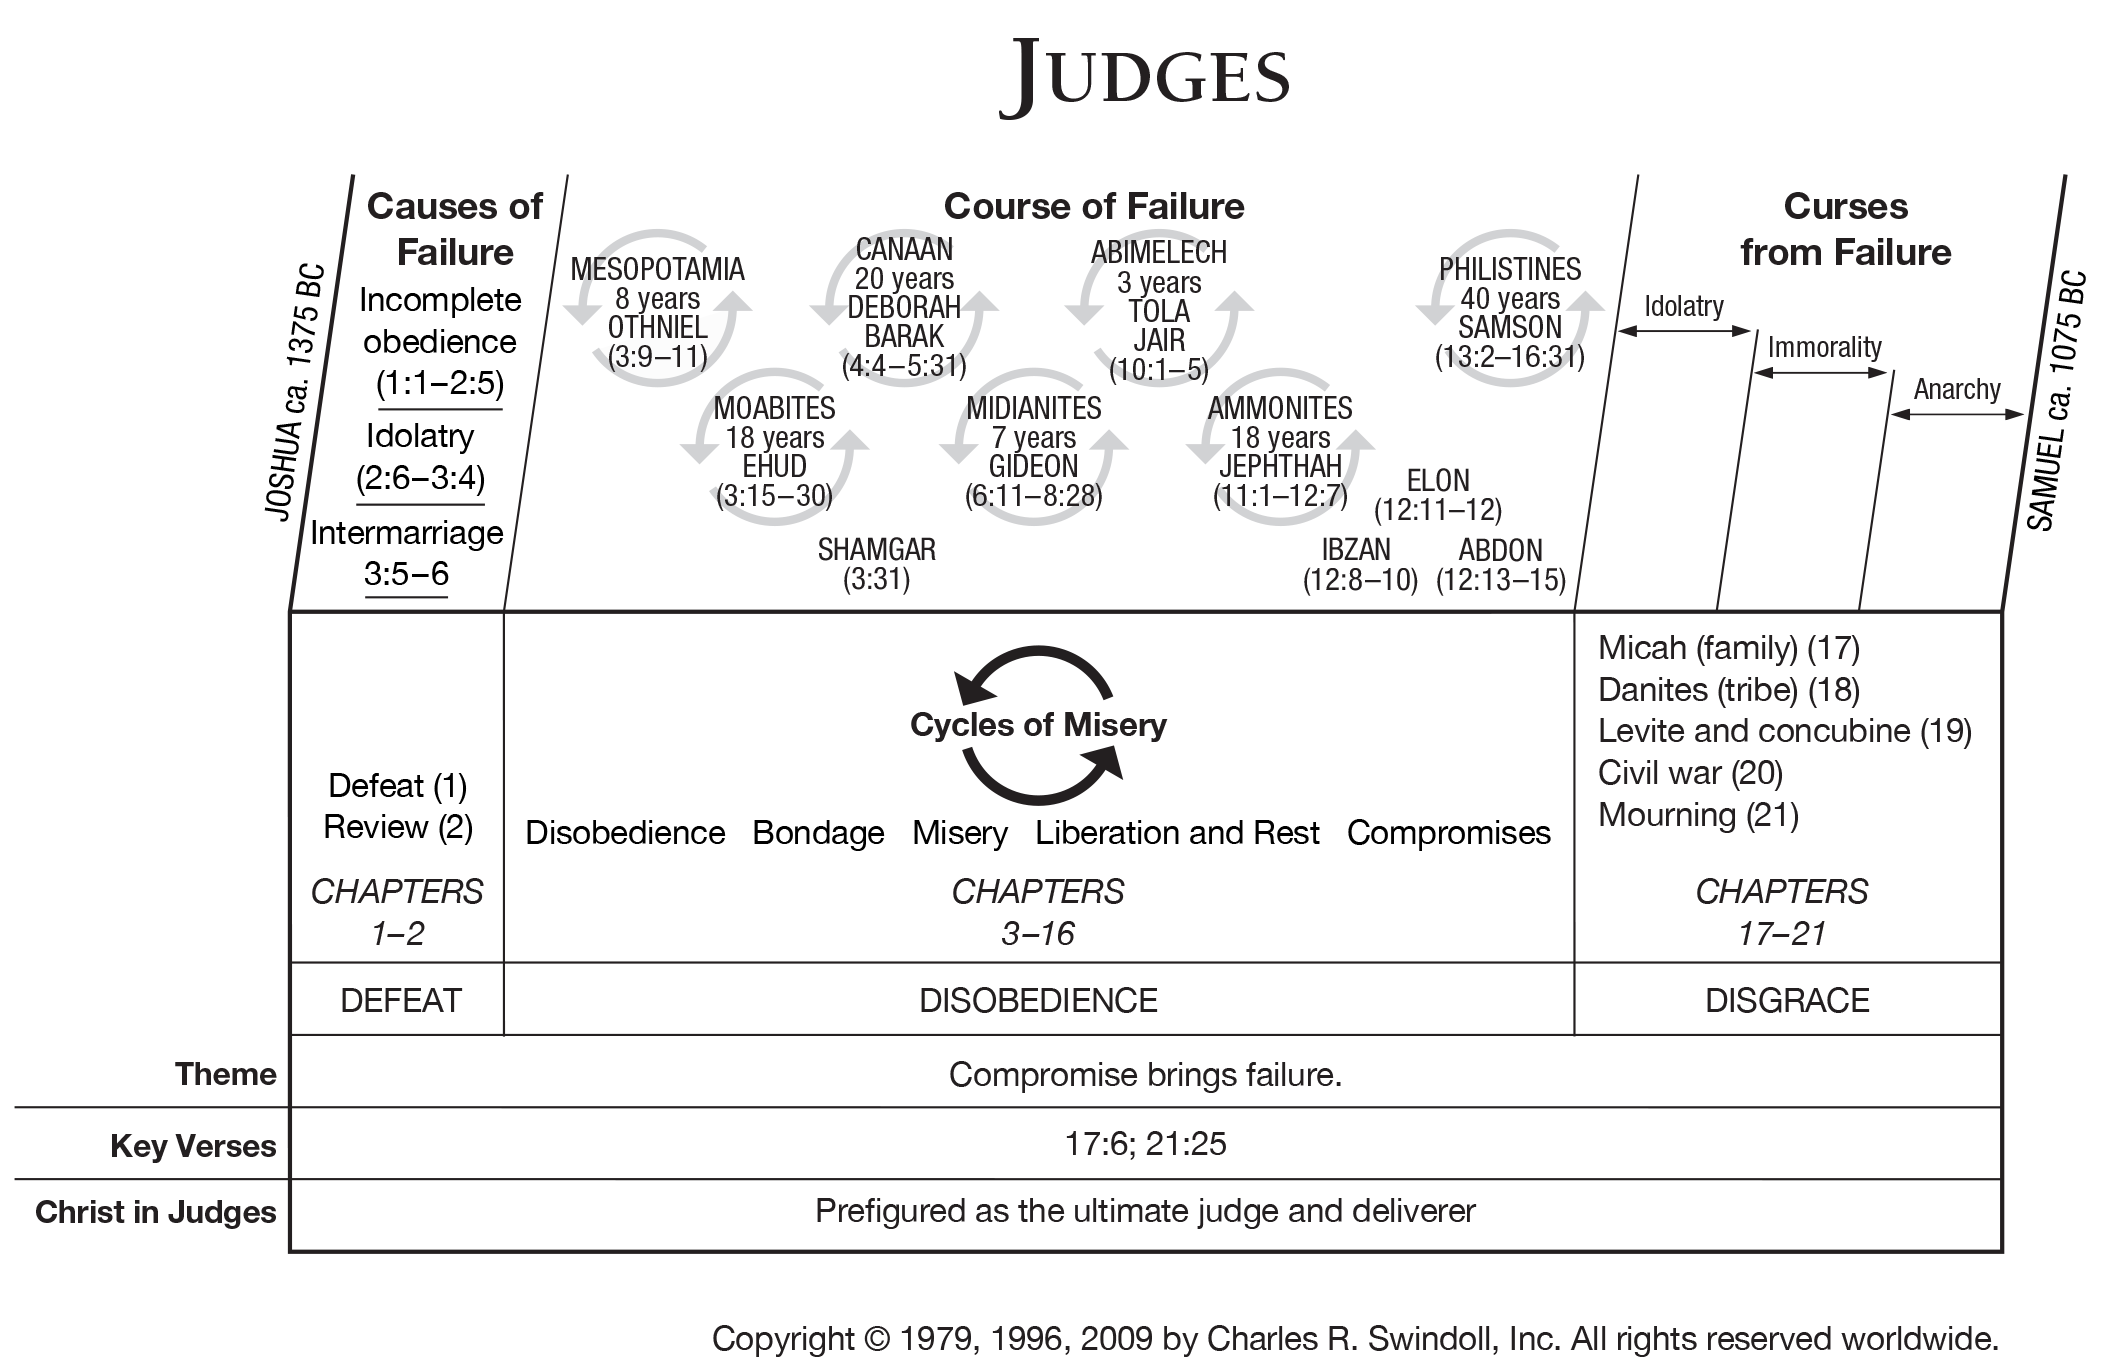
\includegraphics[scale=0.25, angle=90]{07OT-Judges/References/1.Judges-Swindoll}
\caption[Judges from Swindoll]{Judges from Swindoll}
\label{fig:Judges from Swindoll}
\end{center}
\end{figure}


%\newpage
%\begin{figure}
%\begin{center}
%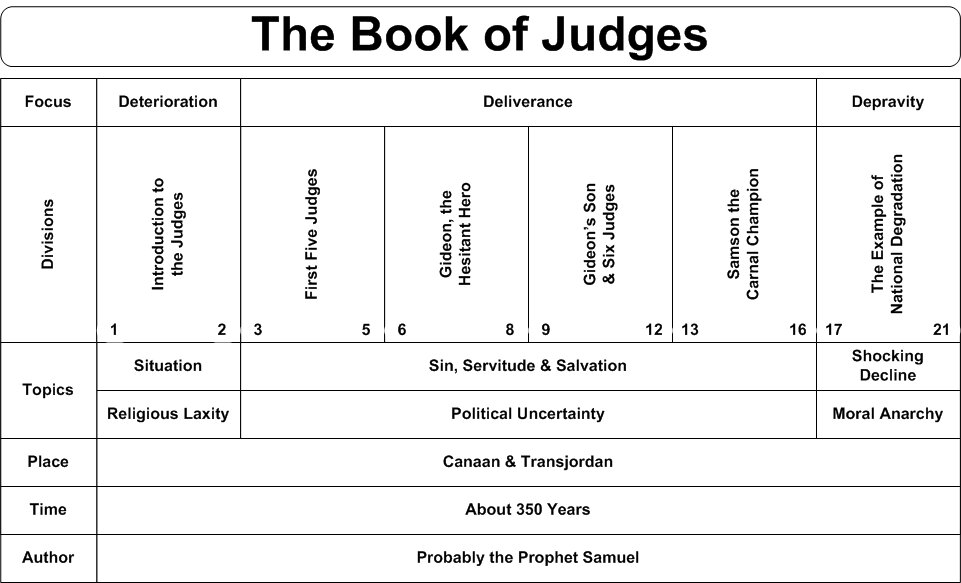
\includegraphics[scale=0.1, angle=0]{07OT-Judges/References/9.Swartzentrover-Judges}
%\caption[Judges from Swartzentrover]{Judges from Swartzentrover}
%\label{fig:Judges from Swartzentrover}
%\end{center}
%\end{figure}


\newpage
\begin{figure}
\begin{center}
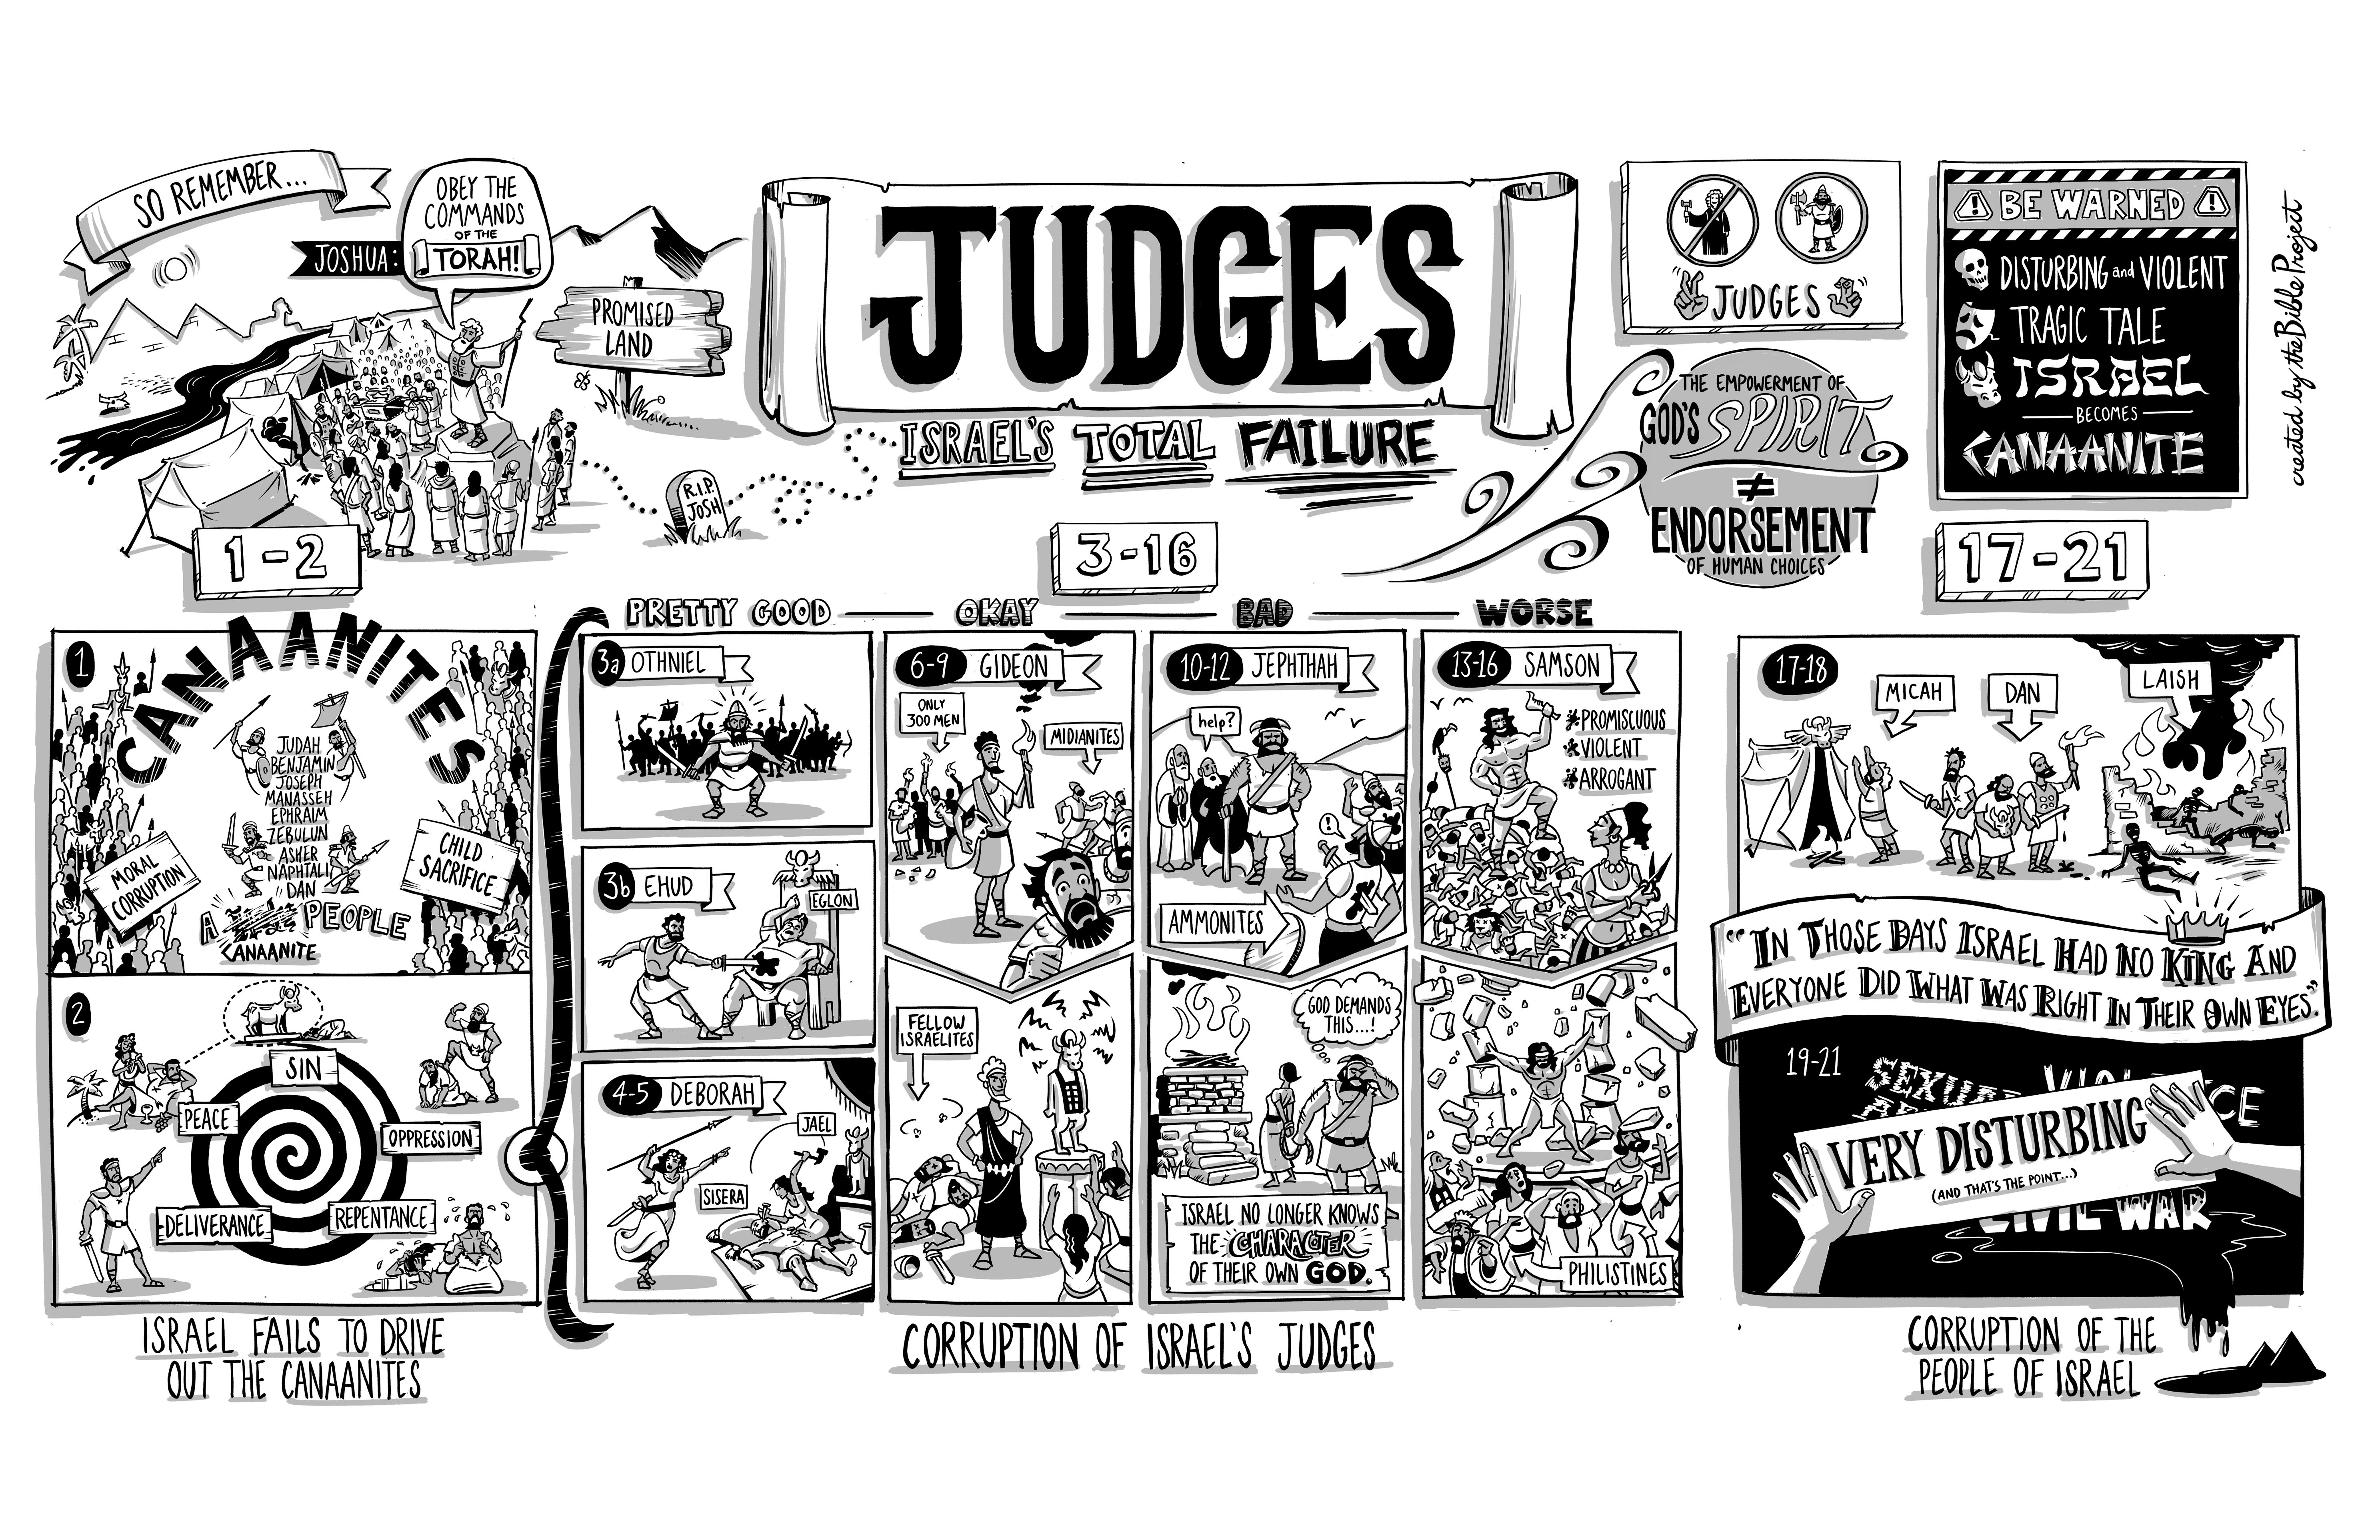
\includegraphics[scale=0.5, angle=90]{07OT-Judges/References/2.BibleProject-Judges}
\caption[Judges from the Bible Project]{Judges from the Bible Project}
\label{fig:Judges from the Bible Project}
\end{center}
\end{figure}


\newpage
\begin{figure}
\begin{center}
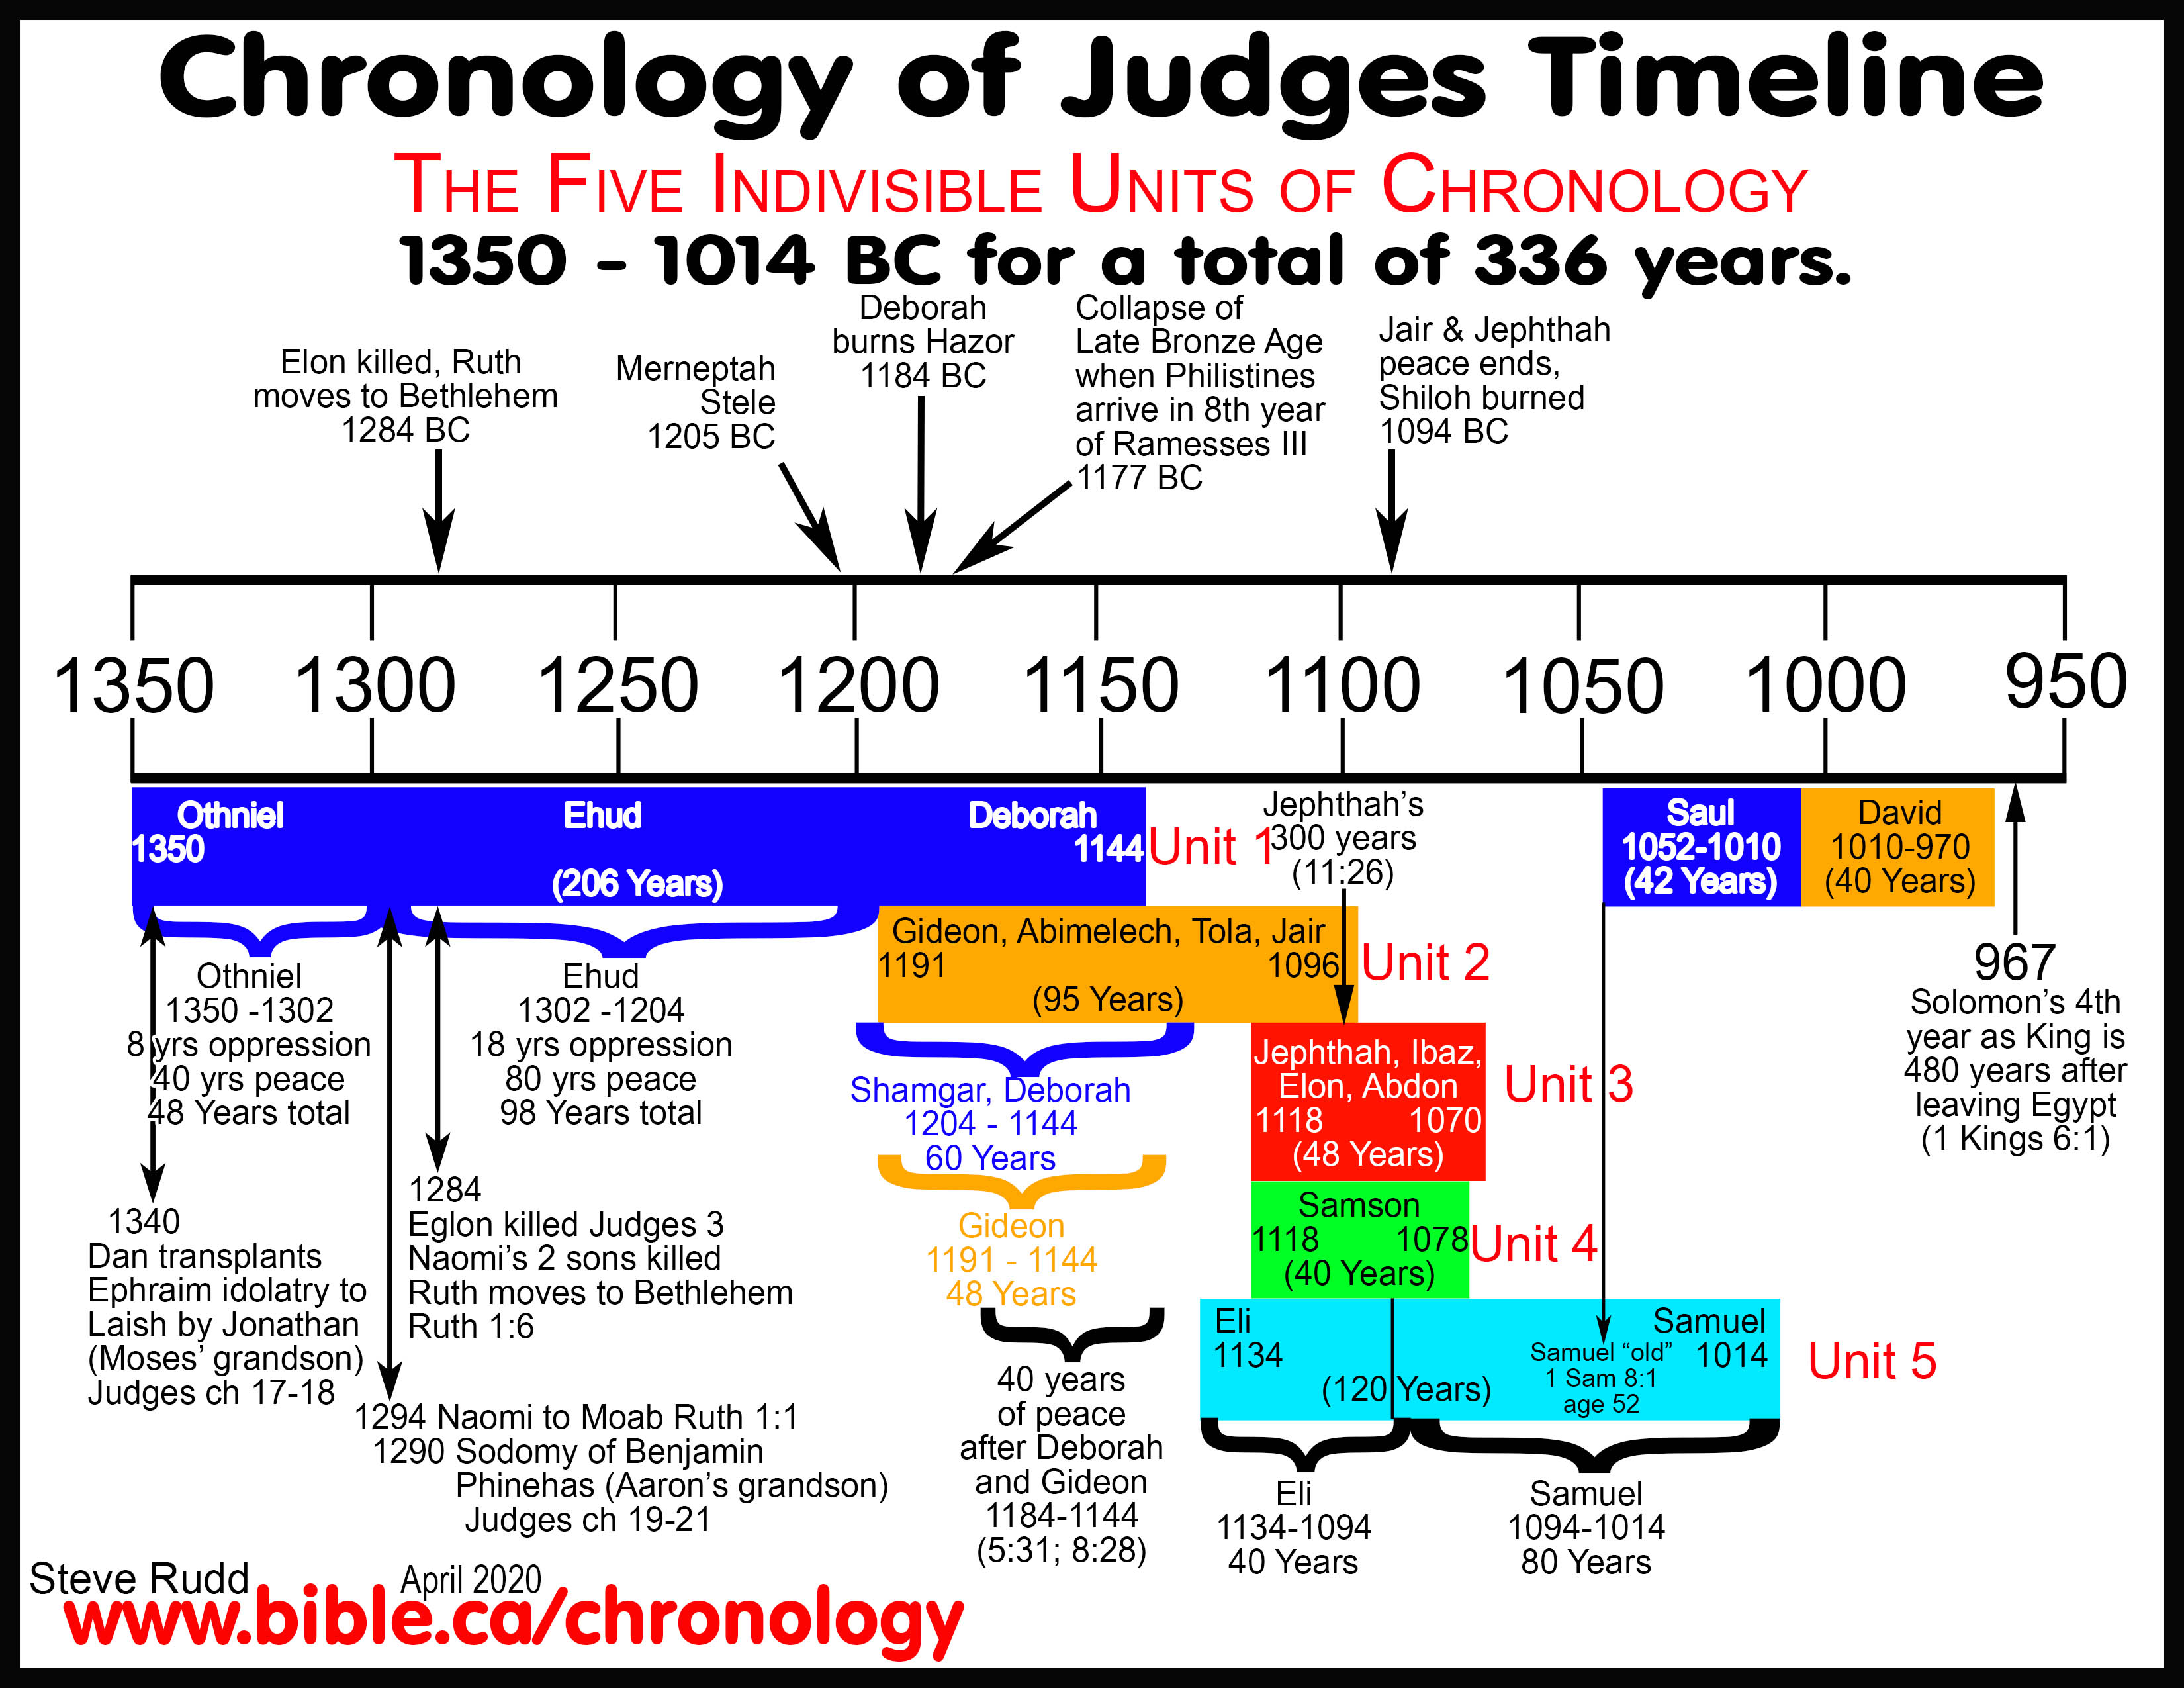
\includegraphics[scale=0.6, angle=90]{07OT-Judges/References/3.Chronology-Judges}
\caption[Chronology of Judges]{Chronology of Judges}
\label{fig:Chronology of Judges}
\end{center}
\end{figure}


\newpage
\begin{figure}
\begin{center}
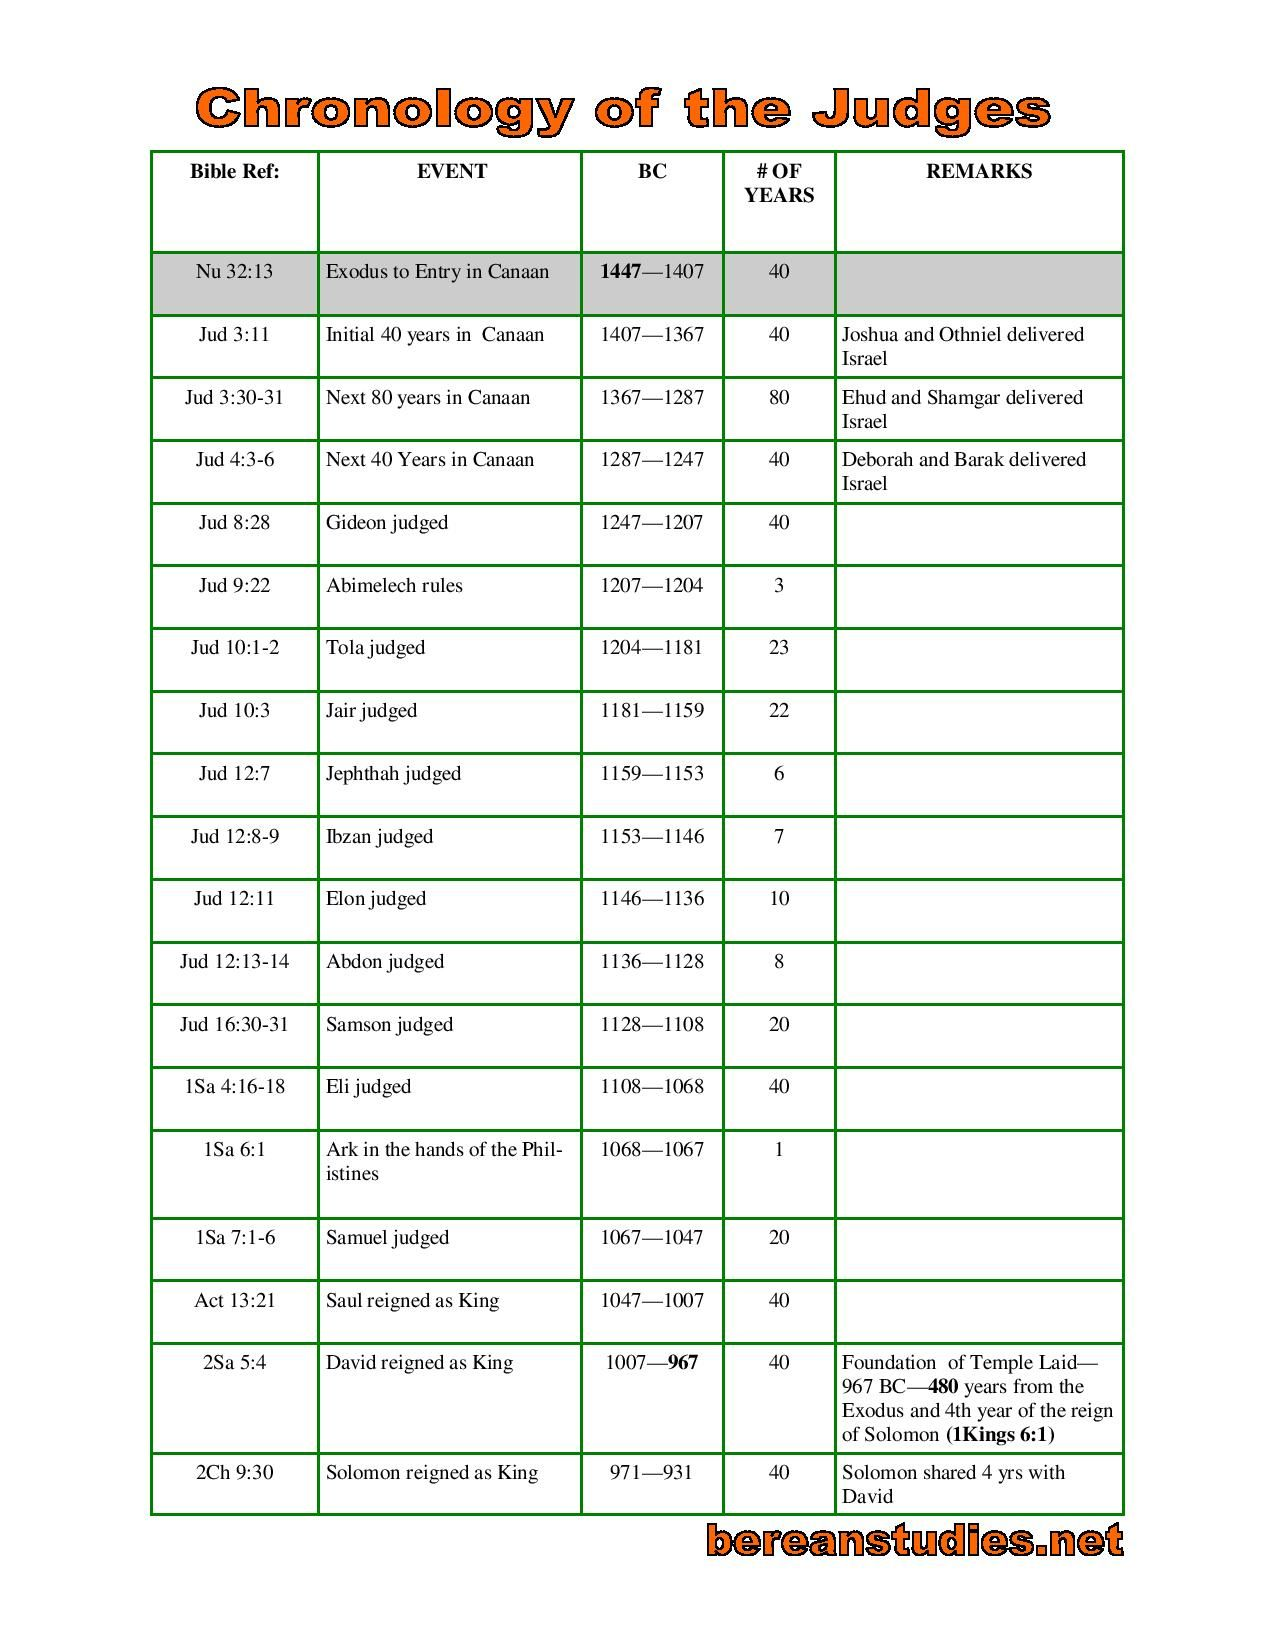
\includegraphics[scale=0.6, angle=0]{07OT-Judges/References/4.Chronology2-Judges}
\caption[Another Chronology of Judges]{Another Chronology of Judges}
\label{fig:Another Chronology of Judges}
\end{center}
\end{figure}

\newpage
\begin{figure}
\begin{center}
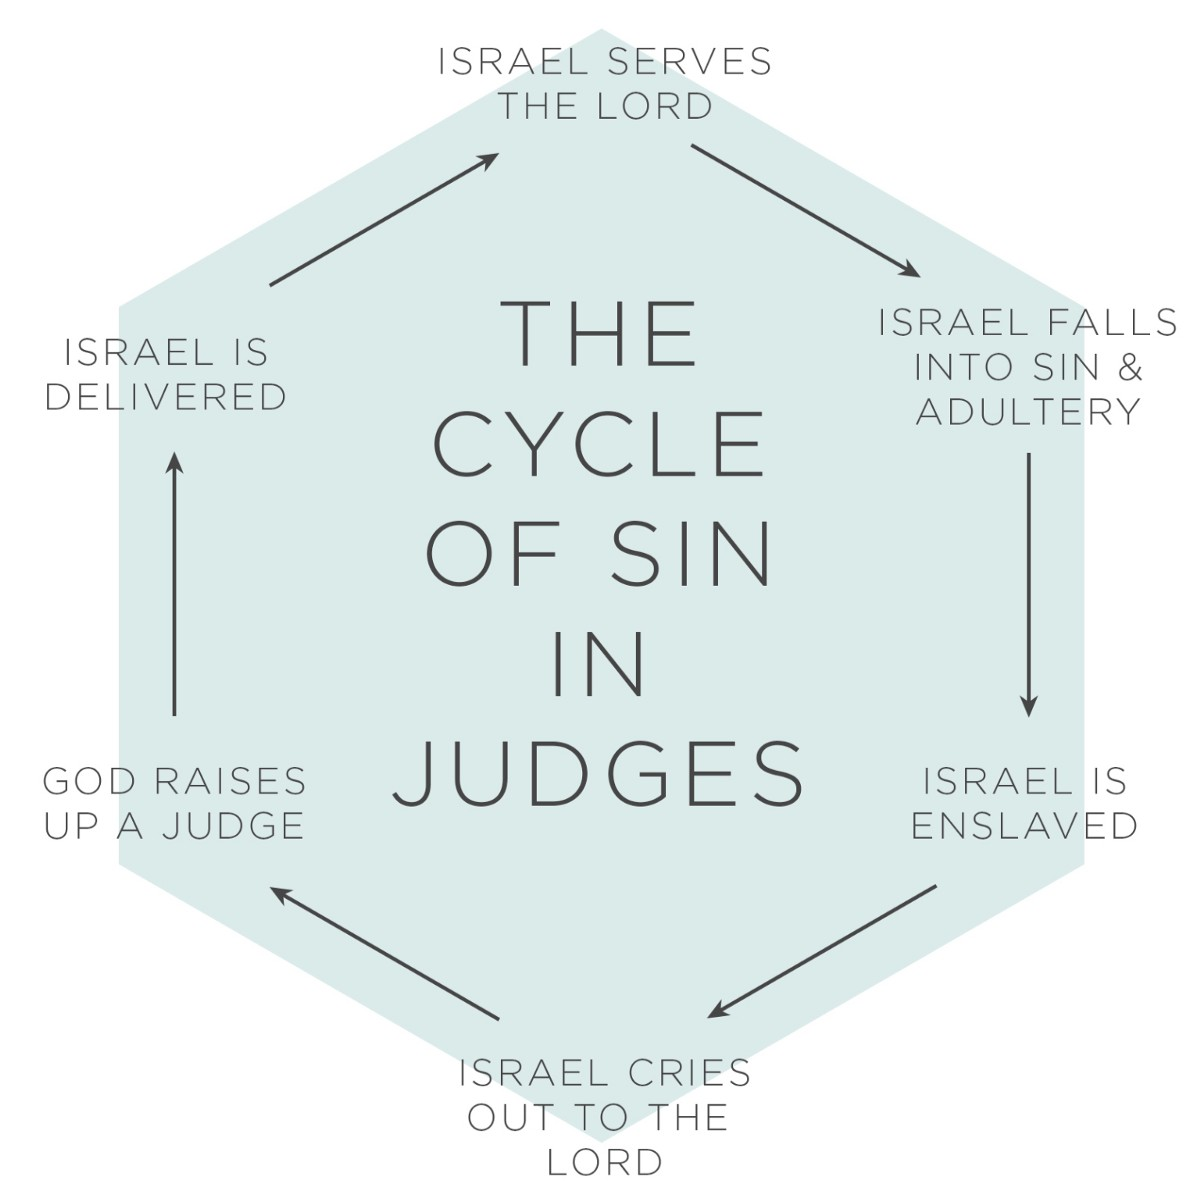
\includegraphics[scale=0.3, angle=0]{07OT-Judges/References/5.Cycles-Judges}
\caption[Cycle of Judges]{Cycle of Judges}
\label{fig:Cycle of Judges}
\end{center}
\end{figure}


\newpage
\begin{figure}
\begin{center}
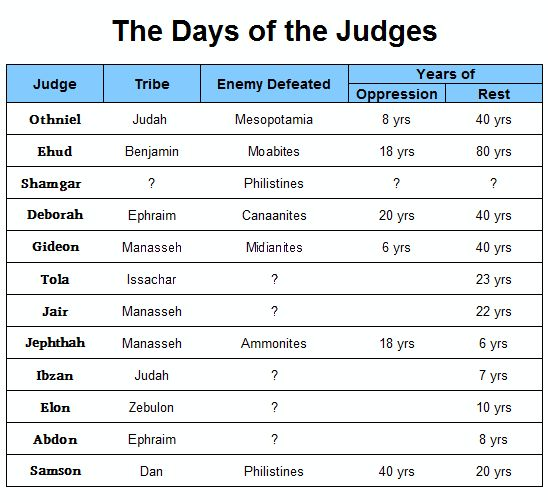
\includegraphics[scale=0.7, angle=0]{07OT-Judges/References/6.DaysOfJudges}
\caption[The Days of the Judges]{The Days of the Judges}
\label{fig:The Days of the Judges}
\end{center}
\end{figure}


\newpage
\begin{figure}
\begin{center}
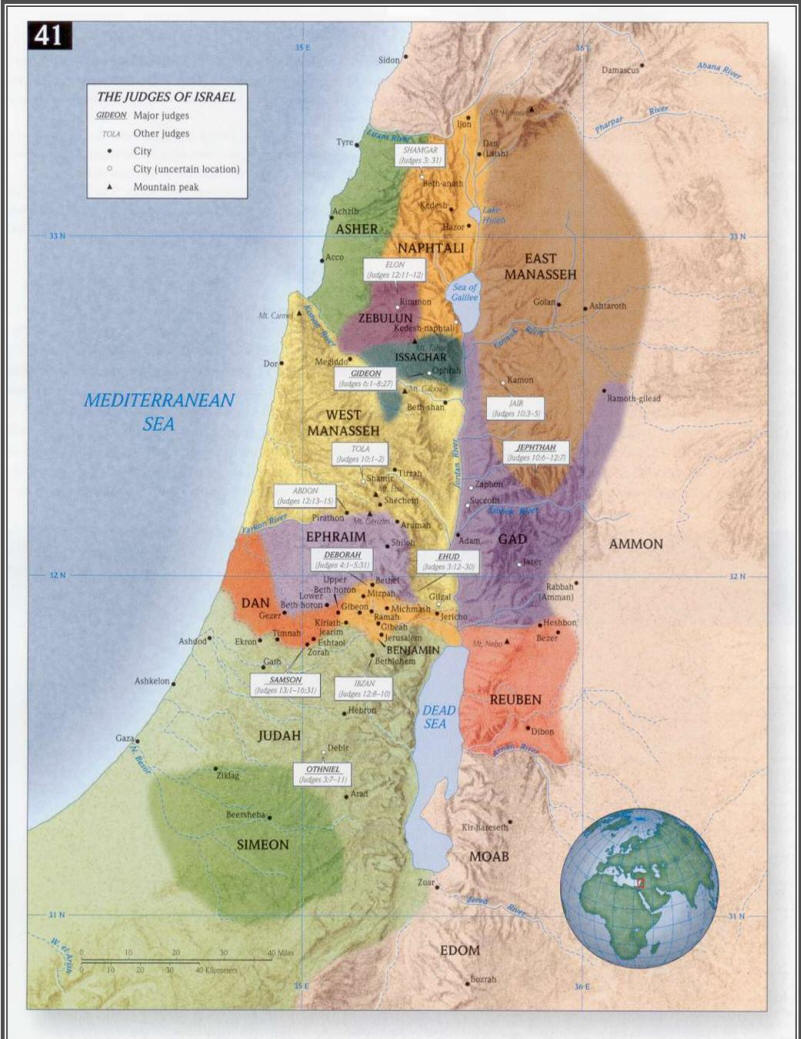
\includegraphics[scale=0.8, angle=0]{07OT-Judges/References/7.Map-Judges}
\caption[Map of the Judges]{Map of the Judges}
\label{fig:Map of the Judges}
\end{center}
\end{figure}


\newpage
\begin{figure}
\begin{center}
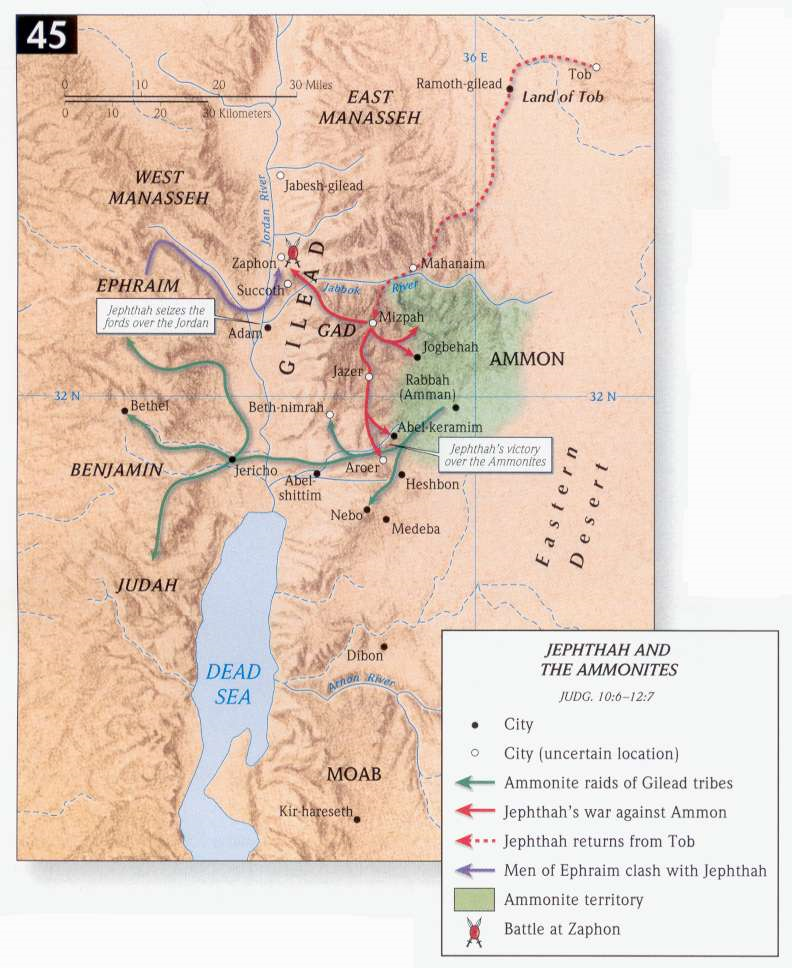
\includegraphics[scale=0.6, angle=0]{07OT-Judges/References/8.Jephthah-Map}
\caption[Map of Jephthah]{Map of Jephthah}
\label{fig:Map of Jephthah}
\end{center}
\end{figure}


\newpage
\begin{figure}
\begin{center}
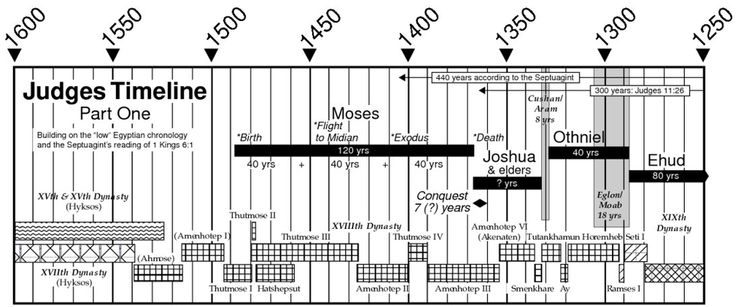
\includegraphics[scale=0.8, angle=90]{07OT-Judges/References/10.Timeline1-Judges}
\caption[Timeline of Judges]{Timeline of Judges}
\label{fig:Timeline of Judges}
\end{center}
\end{figure}



\newpage
\begin{figure}
\begin{center}
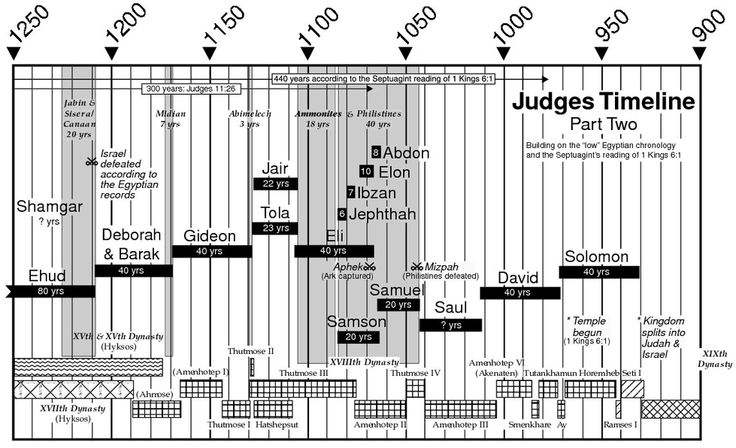
\includegraphics[scale=0.6, angle=90]{07OT-Judges/References/11.Timeline2-Judges}
\caption[Timeline2 of Judges]{Timeline2 of Judges}
\label{fig:Timeline2 of Judges}
\end{center}
\end{figure}


\newpage
\begin{figure}
\begin{center}
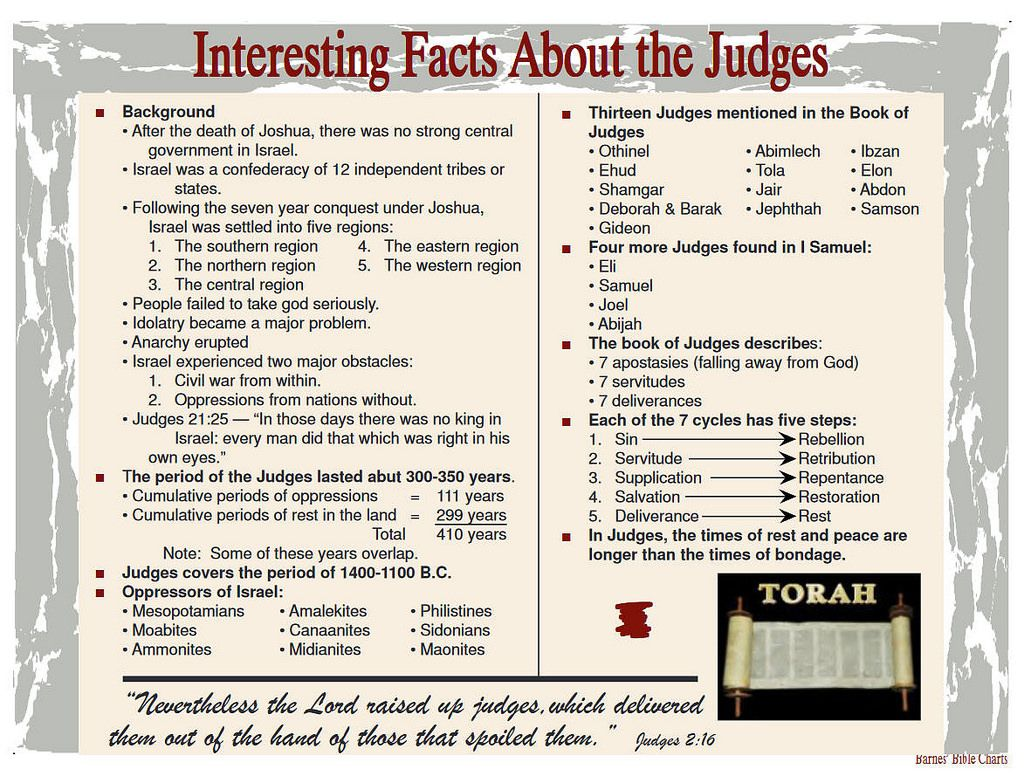
\includegraphics[scale=0.6, angle=90]{07OT-Judges/References/14.InterestingFactsonJudges}
\caption[Interesting Facts about Judges]{Interesting Facts about Judges}
\label{fig:Interesting Facts about Judges}
\end{center}
\end{figure}



\chapter{Judges 4}

\begin{figure}
  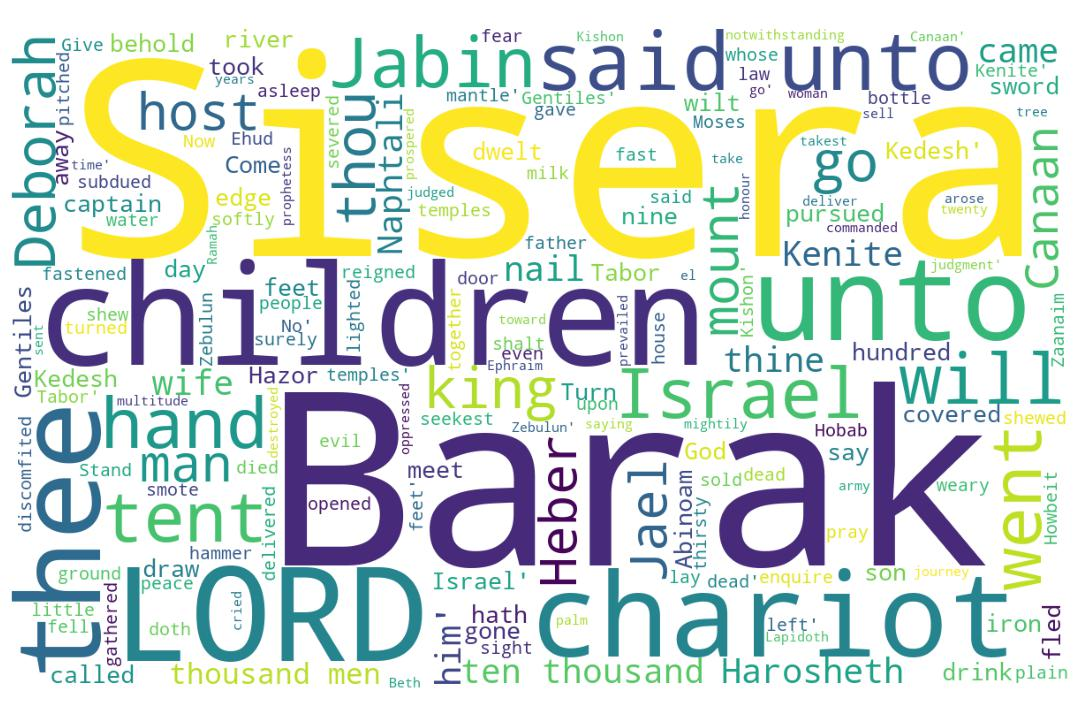
\includegraphics[width=\linewidth]{07OT-Judges/Judges4-WordCloud.jpg}
  \caption{Judges 4 Word Cloud}
  \label{fig:Judges 4 Word Cloud}
\end{figure}


\marginpar{\scriptsize \centering \fcolorbox{bone}{lime}{\textbf{YET AGAIN}}\\ (Judges 4) \begin{compactenum}[I.][8]
    \item   A New  \textbf{Chapter}  \index[scripture]{Judges!Jdg 04:01} (Jdg 4:1) 
    \item   Same  \textbf{Choices}  \index[scripture]{Judges!Jdg 04:01} (Jdg 4:1) 
    \item   The Lord's \textbf{Command}   \index[scripture]{Judges!Jdg 04:06}    (Jdg 4:6) 
    \item   The Enemy  \textbf{Captain}  \index[scripture]{Judges!Jdg 04:06} (Jdg 6:6) 
    \item   The   \textbf{Calls}  \index[scripture]{Judges!Jdg 04:06} \index[scripture]{Judges!Jdg 04:10} (Jdg 4:6, 10) 
    \item   A  \textbf{Champion}  \index[scripture]{Judges!Jdg 04:09} (Jdg 4:9) 
    \item   The  \textbf{Chariots}  \index[scripture]{Judges!Jdg 04:13} (Jdg 4:13) 
\end{compactenum}}


\footnote{\textcolor[rgb]{0.00,0.25,0.00}{\hyperlink{JudgesTOC}{Return to end of Table of Contents.}}}\footnote{\href{https://audiobible.com/bible/judges_4.html}{\textcolor[cmyk]{0.99998,1,0,0}{Judges 4 Audio}}}\textcolor[cmyk]{0.99998,1,0,0}{And the children of Israel \fcolorbox{bone}{lime}{again} did \fcolorbox{bone}{lime}{evil} in the sight of the LORD, when Ehud was dead.}
[2] \textcolor[cmyk]{0.99998,1,0,0}{And the LORD sold them into the hand of Jabin king of Canaan, that reigned in Hazor; the captain of whose host \emph{was} \fcolorbox{bone}{bone}{Sisera}, which dwelt in Harosheth of the Gentiles.}
[3] \textcolor[cmyk]{0.99998,1,0,0}{And the children of Israel cried unto the LORD: for he had nine hundred chariots of iron; and twenty years he mightily oppressed the children of Israel.}\\
\\
\P \textcolor[cmyk]{0.99998,1,0,0}{And Deborah, a prophetess, the wife of Lapidoth, she judged Israel at that time.}
[5] \textcolor[cmyk]{0.99998,1,0,0}{And she dwelt under the palm tree of Deborah between Ramah and Beth-el in mount Ephraim: and the children of Israel came up to her for judgment.}
[6] \textcolor[cmyk]{0.99998,1,0,0}{And she sent and called Barak the son of Abinoam out of Kedesh-naphtali, and said unto him, Hath not the LORD God of Israel \fcolorbox{bone}{lime}{commanded}, \emph{saying}, Go and draw toward mount Tabor, and take with thee ten thousand men of the children of Naphtali and of the children of Zebulun?}
[7] \textcolor[cmyk]{0.99998,1,0,0}{And I will draw unto thee to the river Kishon \fcolorbox{bone}{bone}{Sisera}, the captain of Jabin's army, with his chariots and his multitude; and I will deliver him into thine hand.}
[8] \textcolor[cmyk]{0.99998,1,0,0}{And Barak said unto her, If thou wilt go with me, then I will go: but if thou wilt not go with me, \emph{then} I will not go.}
[9] \textcolor[cmyk]{0.99998,1,0,0}{And she said, I will surely go with thee: notwithstanding the journey that thou takest shall not be for thine honour; for the LORD shall sell \fcolorbox{bone}{bone}{Sisera} into the hand of a woman. And \fcolorbox{bone}{lime}{Deborah} arose, and went with Barak to Kedesh.}\\
\\
\P \textcolor[cmyk]{0.99998,1,0,0}{And Barak \fcolorbox{bone}{lime}{called} Zebulun and Naphtali to Kedesh; and he went up with ten thousand men at his feet: and Deborah went up with him.}
[11] \textcolor[cmyk]{0.99998,1,0,0}{Now Heber the Kenite, \emph{which} \emph{was} of the children of Hobab the father in law of Moses, had severed himself from the Kenites, and pitched his tent unto the plain of Zaanaim, which \emph{is} by Kedesh.}
[12] \textcolor[cmyk]{0.99998,1,0,0}{And they shewed \fcolorbox{bone}{bone}{Sisera} that Barak the son of Abinoam was gone up to mount Tabor.}
[13] \textcolor[cmyk]{0.99998,1,0,0}{And \fcolorbox{bone}{bone}{Sisera} gathered together all his \fcolorbox{bone}{lime}{chariots}, \emph{even} nine hundred chariots of iron, and all the people that \emph{were} with him, from Harosheth of the Gentiles unto the river of Kishon.}\
[14] \textcolor[cmyk]{0.99998,1,0,0}{And Deborah said unto Barak, Up; for this \emph{is} the day in which the LORD hath delivered \fcolorbox{bone}{bone}{Sisera} into thine hand: is not the LORD gone out before thee? So Barak went down from mount Tabor, and ten thousand men after him.}
[15] \textcolor[cmyk]{0.99998,1,0,0}{And the LORD discomfited \fcolorbox{bone}{bone}{Sisera}, and all \emph{his} chariots, and all \emph{his} host, with the edge of the sword before Barak; so that \fcolorbox{bone}{bone}{Sisera} lighted down off \emph{his} chariot, and fled away on his feet.}
[16] \textcolor[cmyk]{0.99998,1,0,0}{But Barak pursued after the chariots, and after the host, unto Harosheth of the Gentiles: and all the host of \fcolorbox{bone}{bone}{Sisera} fell upon the edge of the sword; \emph{and} there was not a man left.}
[17] \textcolor[cmyk]{0.99998,1,0,0}{Howbeit \fcolorbox{bone}{bone}{Sisera} fled away on his feet to the tent of Jael the wife of Heber the Kenite: for \emph{there} \emph{was} peace between Jabin the king of Hazor and the house of Heber the Kenite.}\\
\\
\P \textcolor[cmyk]{0.99998,1,0,0}{And Jael went out to meet \fcolorbox{bone}{bone}{Sisera}, and said unto him, Turn in, my lord, turn in to me; fear not. And when he had turned in unto her into the tent, she covered him with a mantle.}
[19] \textcolor[cmyk]{0.99998,1,0,0}{And he said unto her, Give me, I pray thee, a little water to drink; for I am thirsty. And she opened a bottle of milk, and gave him drink, and covered him.}
[20] \textcolor[cmyk]{0.99998,1,0,0}{Again he said unto her, Stand in the door of the tent, and it shall be, when any man doth come and enquire of thee, and say, Is there any man here? that thou shalt say, No.}
[21] \textcolor[cmyk]{0.99998,1,0,0}{Then Jael Heber's wife took a nail of the tent, and took an hammer in her hand, and went softly unto him, and smote the nail into his temples, and fastened it into the ground: for he was fast asleep and weary. So he died.}
[22] \textcolor[cmyk]{0.99998,1,0,0}{And, behold, as Barak pursued \fcolorbox{bone}{bone}{Sisera}, Jael came out to meet him, and said unto him, Come, and I will shew thee the man whom thou seekest. And when he came into her \emph{tent}, behold, \fcolorbox{bone}{bone}{Sisera} lay dead, and the nail \emph{was} in his temples.}
[23] \textcolor[cmyk]{0.99998,1,0,0}{So God subdued on that day Jabin the king of Canaan before the children of Israel.}
[24] \textcolor[cmyk]{0.99998,1,0,0}{And the hand of the children of Israel prospered, and prevailed against Jabin the king of Canaan, until they had destroyed Jabin king of Canaan.}
\index[NWIV]{18!Judges!Jud 4:1}\index[AWIP]{And!Judges!Jud 4:1}\index[AWIP]{the!Judges!Jud 4:1}\index[AWIP]{the!Judges!Jud 4:1 (2)}\index[AWIP]{the!Judges!Jud 4:1 (3)}\index[AWIP]{children!Judges!Jud 4:1}\index[AWIP]{of!Judges!Jud 4:1}\index[AWIP]{of!Judges!Jud 4:1 (2)}\index[AWIP]{Israel!Judges!Jud 4:1}\index[AWIP]{again!Judges!Jud 4:1}\index[AWIP]{did!Judges!Jud 4:1}\index[AWIP]{evil!Judges!Jud 4:1}\index[AWIP]{in!Judges!Jud 4:1}\index[AWIP]{sight!Judges!Jud 4:1}\index[AWIP]{LORD!Judges!Jud 4:1}\index[AWIP]{when!Judges!Jud 4:1}\index[AWIP]{Ehud!Judges!Jud 4:1}\index[AWIP]{was!Judges!Jud 4:1}\index[AWIP]{dead!Judges!Jud 4:1}

\index[NWIV]{31!Judges!Jud 4:2}\index[AWIP]{And!Judges!Jud 4:2}\index[AWIP]{the!Judges!Jud 4:2}\index[AWIP]{the!Judges!Jud 4:2 (2)}\index[AWIP]{the!Judges!Jud 4:2 (3)}\index[AWIP]{the!Judges!Jud 4:2 (4)}\index[AWIP]{LORD!Judges!Jud 4:2}\index[AWIP]{sold!Judges!Jud 4:2}\index[AWIP]{them!Judges!Jud 4:2}\index[AWIP]{into!Judges!Jud 4:2}\index[AWIP]{hand!Judges!Jud 4:2}\index[AWIP]{of!Judges!Jud 4:2}\index[AWIP]{of!Judges!Jud 4:2 (2)}\index[AWIP]{of!Judges!Jud 4:2 (3)}\index[AWIP]{of!Judges!Jud 4:2 (4)}\index[AWIP]{Jabin!Judges!Jud 4:2}\index[AWIP]{king!Judges!Jud 4:2}\index[AWIP]{Canaan!Judges!Jud 4:2}\index[AWIP]{that!Judges!Jud 4:2}\index[AWIP]{reigned!Judges!Jud 4:2}\index[AWIP]{in!Judges!Jud 4:2}\index[AWIP]{in!Judges!Jud 4:2 (2)}\index[AWIP]{Hazor!Judges!Jud 4:2}\index[AWIP]{captain!Judges!Jud 4:2}\index[AWIP]{whose!Judges!Jud 4:2}\index[AWIP]{host!Judges!Jud 4:2}\index[AWIP]{\emph{was}!Judges!Jud 4:2}\index[AWIP]{Sisera!Judges!Jud 4:2}\index[AWIP]{which!Judges!Jud 4:2}\index[AWIP]{dwelt!Judges!Jud 4:2}\index[AWIP]{Harosheth!Judges!Jud 4:2}\index[AWIP]{Gentiles!Judges!Jud 4:2}\index[AWIP]{\emph{was}!Judges!Jud 4:2}

\index[NWIV]{27!Judges!Jud 4:3}\index[AWIP]{And!Judges!Jud 4:3}\index[AWIP]{the!Judges!Jud 4:3}\index[AWIP]{the!Judges!Jud 4:3 (2)}\index[AWIP]{the!Judges!Jud 4:3 (3)}\index[AWIP]{children!Judges!Jud 4:3}\index[AWIP]{children!Judges!Jud 4:3 (2)}\index[AWIP]{of!Judges!Jud 4:3}\index[AWIP]{of!Judges!Jud 4:3 (2)}\index[AWIP]{of!Judges!Jud 4:3 (3)}\index[AWIP]{Israel!Judges!Jud 4:3}\index[AWIP]{Israel!Judges!Jud 4:3 (2)}\index[AWIP]{cried!Judges!Jud 4:3}\index[AWIP]{unto!Judges!Jud 4:3}\index[AWIP]{LORD!Judges!Jud 4:3}\index[AWIP]{for!Judges!Jud 4:3}\index[AWIP]{he!Judges!Jud 4:3}\index[AWIP]{he!Judges!Jud 4:3 (2)}\index[AWIP]{had!Judges!Jud 4:3}\index[AWIP]{nine!Judges!Jud 4:3}\index[AWIP]{hundred!Judges!Jud 4:3}\index[AWIP]{chariots!Judges!Jud 4:3}\index[AWIP]{iron!Judges!Jud 4:3}\index[AWIP]{and!Judges!Jud 4:3}\index[AWIP]{twenty!Judges!Jud 4:3}\index[AWIP]{years!Judges!Jud 4:3}\index[AWIP]{mightily!Judges!Jud 4:3}\index[AWIP]{oppressed!Judges!Jud 4:3}

\index[NWIV]{14!Judges!Jud 4:4}\index[AWIP]{And!Judges!Jud 4:4}\index[AWIP]{Deborah!Judges!Jud 4:4}\index[AWIP]{a!Judges!Jud 4:4}\index[AWIP]{prophetess!Judges!Jud 4:4}\index[AWIP]{the!Judges!Jud 4:4}\index[AWIP]{wife!Judges!Jud 4:4}\index[AWIP]{of!Judges!Jud 4:4}\index[AWIP]{Lapidoth!Judges!Jud 4:4}\index[AWIP]{she!Judges!Jud 4:4}\index[AWIP]{judged!Judges!Jud 4:4}\index[AWIP]{Israel!Judges!Jud 4:4}\index[AWIP]{at!Judges!Jud 4:4}\index[AWIP]{that!Judges!Jud 4:4}\index[AWIP]{time!Judges!Jud 4:4}

\index[NWIV]{27!Judges!Jud 4:5}\index[AWIP]{And!Judges!Jud 4:5}\index[AWIP]{she!Judges!Jud 4:5}\index[AWIP]{dwelt!Judges!Jud 4:5}\index[AWIP]{under!Judges!Jud 4:5}\index[AWIP]{the!Judges!Jud 4:5}\index[AWIP]{the!Judges!Jud 4:5 (2)}\index[AWIP]{palm!Judges!Jud 4:5}\index[AWIP]{tree!Judges!Jud 4:5}\index[AWIP]{of!Judges!Jud 4:5}\index[AWIP]{of!Judges!Jud 4:5 (2)}\index[AWIP]{Deborah!Judges!Jud 4:5}\index[AWIP]{between!Judges!Jud 4:5}\index[AWIP]{Ramah!Judges!Jud 4:5}\index[AWIP]{and!Judges!Jud 4:5}\index[AWIP]{and!Judges!Jud 4:5 (2)}\index[AWIP]{Beth-el!Judges!Jud 4:5}\index[AWIP]{in!Judges!Jud 4:5}\index[AWIP]{mount!Judges!Jud 4:5}\index[AWIP]{Ephraim!Judges!Jud 4:5}\index[AWIP]{children!Judges!Jud 4:5}\index[AWIP]{Israel!Judges!Jud 4:5}\index[AWIP]{came!Judges!Jud 4:5}\index[AWIP]{up!Judges!Jud 4:5}\index[AWIP]{to!Judges!Jud 4:5}\index[AWIP]{her!Judges!Jud 4:5}\index[AWIP]{for!Judges!Jud 4:5}\index[AWIP]{judgment!Judges!Jud 4:5}

\index[NWIV]{50!Judges!Jud 4:6}\index[AWIP]{And!Judges!Jud 4:6}\index[AWIP]{she!Judges!Jud 4:6}\index[AWIP]{sent!Judges!Jud 4:6}\index[AWIP]{and!Judges!Jud 4:6}\index[AWIP]{and!Judges!Jud 4:6 (2)}\index[AWIP]{and!Judges!Jud 4:6 (3)}\index[AWIP]{and!Judges!Jud 4:6 (4)}\index[AWIP]{and!Judges!Jud 4:6 (5)}\index[AWIP]{called!Judges!Jud 4:6}\index[AWIP]{Barak!Judges!Jud 4:6}\index[AWIP]{the!Judges!Jud 4:6}\index[AWIP]{the!Judges!Jud 4:6 (2)}\index[AWIP]{the!Judges!Jud 4:6 (3)}\index[AWIP]{the!Judges!Jud 4:6 (4)}\index[AWIP]{son!Judges!Jud 4:6}\index[AWIP]{of!Judges!Jud 4:6}\index[AWIP]{of!Judges!Jud 4:6 (2)}\index[AWIP]{of!Judges!Jud 4:6 (3)}\index[AWIP]{of!Judges!Jud 4:6 (4)}\index[AWIP]{of!Judges!Jud 4:6 (5)}\index[AWIP]{of!Judges!Jud 4:6 (6)}\index[AWIP]{of!Judges!Jud 4:6 (7)}\index[AWIP]{Abinoam!Judges!Jud 4:6}\index[AWIP]{out!Judges!Jud 4:6}\index[AWIP]{Kedesh-naphtali!Judges!Jud 4:6}\index[AWIP]{said!Judges!Jud 4:6}\index[AWIP]{unto!Judges!Jud 4:6}\index[AWIP]{him!Judges!Jud 4:6}\index[AWIP]{Hath!Judges!Jud 4:6}\index[AWIP]{not!Judges!Jud 4:6}\index[AWIP]{LORD!Judges!Jud 4:6}\index[AWIP]{God!Judges!Jud 4:6}\index[AWIP]{Israel!Judges!Jud 4:6}\index[AWIP]{commanded!Judges!Jud 4:6}\index[AWIP]{\emph{saying}!Judges!Jud 4:6}\index[AWIP]{Go!Judges!Jud 4:6}\index[AWIP]{draw!Judges!Jud 4:6}\index[AWIP]{toward!Judges!Jud 4:6}\index[AWIP]{mount!Judges!Jud 4:6}\index[AWIP]{Tabor!Judges!Jud 4:6}\index[AWIP]{take!Judges!Jud 4:6}\index[AWIP]{with!Judges!Jud 4:6}\index[AWIP]{thee!Judges!Jud 4:6}\index[AWIP]{ten!Judges!Jud 4:6}\index[AWIP]{thousand!Judges!Jud 4:6}\index[AWIP]{men!Judges!Jud 4:6}\index[AWIP]{children!Judges!Jud 4:6}\index[AWIP]{children!Judges!Jud 4:6 (2)}\index[AWIP]{Naphtali!Judges!Jud 4:6}\index[AWIP]{Zebulun?!Judges!Jud 4:6}\index[AWIP]{\emph{saying}!Judges!Jud 4:6}

\index[NWIV]{30!Judges!Jud 4:7}\index[AWIP]{And!Judges!Jud 4:7}\index[AWIP]{I!Judges!Jud 4:7}\index[AWIP]{I!Judges!Jud 4:7 (2)}\index[AWIP]{will!Judges!Jud 4:7}\index[AWIP]{will!Judges!Jud 4:7 (2)}\index[AWIP]{draw!Judges!Jud 4:7}\index[AWIP]{unto!Judges!Jud 4:7}\index[AWIP]{thee!Judges!Jud 4:7}\index[AWIP]{to!Judges!Jud 4:7}\index[AWIP]{the!Judges!Jud 4:7}\index[AWIP]{the!Judges!Jud 4:7 (2)}\index[AWIP]{river!Judges!Jud 4:7}\index[AWIP]{Kishon!Judges!Jud 4:7}\index[AWIP]{Sisera!Judges!Jud 4:7}\index[AWIP]{captain!Judges!Jud 4:7}\index[AWIP]{of!Judges!Jud 4:7}\index[AWIP]{Jabin's!Judges!Jud 4:7}\index[AWIP]{army!Judges!Jud 4:7}\index[AWIP]{with!Judges!Jud 4:7}\index[AWIP]{his!Judges!Jud 4:7}\index[AWIP]{his!Judges!Jud 4:7 (2)}\index[AWIP]{chariots!Judges!Jud 4:7}\index[AWIP]{and!Judges!Jud 4:7}\index[AWIP]{and!Judges!Jud 4:7 (2)}\index[AWIP]{multitude!Judges!Jud 4:7}\index[AWIP]{deliver!Judges!Jud 4:7}\index[AWIP]{him!Judges!Jud 4:7}\index[AWIP]{into!Judges!Jud 4:7}\index[AWIP]{thine!Judges!Jud 4:7}\index[AWIP]{hand!Judges!Jud 4:7}

\index[NWIV]{28!Judges!Jud 4:8}\index[AWIP]{And!Judges!Jud 4:8}\index[AWIP]{Barak!Judges!Jud 4:8}\index[AWIP]{said!Judges!Jud 4:8}\index[AWIP]{unto!Judges!Jud 4:8}\index[AWIP]{her!Judges!Jud 4:8}\index[AWIP]{If!Judges!Jud 4:8}\index[AWIP]{thou!Judges!Jud 4:8}\index[AWIP]{thou!Judges!Jud 4:8 (2)}\index[AWIP]{wilt!Judges!Jud 4:8}\index[AWIP]{wilt!Judges!Jud 4:8 (2)}\index[AWIP]{go!Judges!Jud 4:8}\index[AWIP]{go!Judges!Jud 4:8 (2)}\index[AWIP]{go!Judges!Jud 4:8 (3)}\index[AWIP]{go!Judges!Jud 4:8 (4)}\index[AWIP]{with!Judges!Jud 4:8}\index[AWIP]{with!Judges!Jud 4:8 (2)}\index[AWIP]{me!Judges!Jud 4:8}\index[AWIP]{me!Judges!Jud 4:8 (2)}\index[AWIP]{then!Judges!Jud 4:8}\index[AWIP]{I!Judges!Jud 4:8}\index[AWIP]{I!Judges!Jud 4:8 (2)}\index[AWIP]{will!Judges!Jud 4:8}\index[AWIP]{will!Judges!Jud 4:8 (2)}\index[AWIP]{but!Judges!Jud 4:8}\index[AWIP]{if!Judges!Jud 4:8}\index[AWIP]{not!Judges!Jud 4:8}\index[AWIP]{not!Judges!Jud 4:8 (2)}\index[AWIP]{\emph{then}!Judges!Jud 4:8}\index[AWIP]{\emph{then}!Judges!Jud 4:8}

\index[NWIV]{42!Judges!Jud 4:9}\index[AWIP]{And!Judges!Jud 4:9}\index[AWIP]{And!Judges!Jud 4:9 (2)}\index[AWIP]{she!Judges!Jud 4:9}\index[AWIP]{said!Judges!Jud 4:9}\index[AWIP]{I!Judges!Jud 4:9}\index[AWIP]{will!Judges!Jud 4:9}\index[AWIP]{surely!Judges!Jud 4:9}\index[AWIP]{go!Judges!Jud 4:9}\index[AWIP]{with!Judges!Jud 4:9}\index[AWIP]{with!Judges!Jud 4:9 (2)}\index[AWIP]{thee!Judges!Jud 4:9}\index[AWIP]{notwithstanding!Judges!Jud 4:9}\index[AWIP]{the!Judges!Jud 4:9}\index[AWIP]{the!Judges!Jud 4:9 (2)}\index[AWIP]{the!Judges!Jud 4:9 (3)}\index[AWIP]{journey!Judges!Jud 4:9}\index[AWIP]{that!Judges!Jud 4:9}\index[AWIP]{thou!Judges!Jud 4:9}\index[AWIP]{takest!Judges!Jud 4:9}\index[AWIP]{shall!Judges!Jud 4:9}\index[AWIP]{shall!Judges!Jud 4:9 (2)}\index[AWIP]{not!Judges!Jud 4:9}\index[AWIP]{be!Judges!Jud 4:9}\index[AWIP]{for!Judges!Jud 4:9}\index[AWIP]{for!Judges!Jud 4:9 (2)}\index[AWIP]{thine!Judges!Jud 4:9}\index[AWIP]{honour!Judges!Jud 4:9}\index[AWIP]{LORD!Judges!Jud 4:9}\index[AWIP]{sell!Judges!Jud 4:9}\index[AWIP]{Sisera!Judges!Jud 4:9}\index[AWIP]{into!Judges!Jud 4:9}\index[AWIP]{hand!Judges!Jud 4:9}\index[AWIP]{of!Judges!Jud 4:9}\index[AWIP]{a!Judges!Jud 4:9}\index[AWIP]{woman!Judges!Jud 4:9}\index[AWIP]{Deborah!Judges!Jud 4:9}\index[AWIP]{arose!Judges!Jud 4:9}\index[AWIP]{and!Judges!Jud 4:9}\index[AWIP]{went!Judges!Jud 4:9}\index[AWIP]{Barak!Judges!Jud 4:9}\index[AWIP]{to!Judges!Jud 4:9}\index[AWIP]{Kedesh!Judges!Jud 4:9}

\index[NWIV]{25!Judges!Jud 4:10}\index[AWIP]{And!Judges!Jud 4:10}\index[AWIP]{Barak!Judges!Jud 4:10}\index[AWIP]{called!Judges!Jud 4:10}\index[AWIP]{Zebulun!Judges!Jud 4:10}\index[AWIP]{and!Judges!Jud 4:10}\index[AWIP]{and!Judges!Jud 4:10 (2)}\index[AWIP]{and!Judges!Jud 4:10 (3)}\index[AWIP]{Naphtali!Judges!Jud 4:10}\index[AWIP]{to!Judges!Jud 4:10}\index[AWIP]{Kedesh!Judges!Jud 4:10}\index[AWIP]{he!Judges!Jud 4:10}\index[AWIP]{went!Judges!Jud 4:10}\index[AWIP]{went!Judges!Jud 4:10 (2)}\index[AWIP]{up!Judges!Jud 4:10}\index[AWIP]{up!Judges!Jud 4:10 (2)}\index[AWIP]{with!Judges!Jud 4:10}\index[AWIP]{with!Judges!Jud 4:10 (2)}\index[AWIP]{ten!Judges!Jud 4:10}\index[AWIP]{thousand!Judges!Jud 4:10}\index[AWIP]{men!Judges!Jud 4:10}\index[AWIP]{at!Judges!Jud 4:10}\index[AWIP]{his!Judges!Jud 4:10}\index[AWIP]{feet!Judges!Jud 4:10}\index[AWIP]{Deborah!Judges!Jud 4:10}\index[AWIP]{him!Judges!Jud 4:10}

\index[NWIV]{36!Judges!Jud 4:11}\index[AWIP]{Now!Judges!Jud 4:11}\index[AWIP]{Heber!Judges!Jud 4:11}\index[AWIP]{the!Judges!Jud 4:11}\index[AWIP]{the!Judges!Jud 4:11 (2)}\index[AWIP]{the!Judges!Jud 4:11 (3)}\index[AWIP]{the!Judges!Jud 4:11 (4)}\index[AWIP]{the!Judges!Jud 4:11 (5)}\index[AWIP]{Kenite!Judges!Jud 4:11}\index[AWIP]{\emph{which}!Judges!Jud 4:11}\index[AWIP]{\emph{was}!Judges!Jud 4:11}\index[AWIP]{of!Judges!Jud 4:11}\index[AWIP]{of!Judges!Jud 4:11 (2)}\index[AWIP]{of!Judges!Jud 4:11 (3)}\index[AWIP]{of!Judges!Jud 4:11 (4)}\index[AWIP]{children!Judges!Jud 4:11}\index[AWIP]{Hobab!Judges!Jud 4:11}\index[AWIP]{father!Judges!Jud 4:11}\index[AWIP]{in!Judges!Jud 4:11}\index[AWIP]{law!Judges!Jud 4:11}\index[AWIP]{Moses!Judges!Jud 4:11}\index[AWIP]{had!Judges!Jud 4:11}\index[AWIP]{severed!Judges!Jud 4:11}\index[AWIP]{himself!Judges!Jud 4:11}\index[AWIP]{from!Judges!Jud 4:11}\index[AWIP]{Kenites!Judges!Jud 4:11}\index[AWIP]{and!Judges!Jud 4:11}\index[AWIP]{pitched!Judges!Jud 4:11}\index[AWIP]{his!Judges!Jud 4:11}\index[AWIP]{tent!Judges!Jud 4:11}\index[AWIP]{unto!Judges!Jud 4:11}\index[AWIP]{plain!Judges!Jud 4:11}\index[AWIP]{Zaanaim!Judges!Jud 4:11}\index[AWIP]{which!Judges!Jud 4:11}\index[AWIP]{\emph{is}!Judges!Jud 4:11}\index[AWIP]{by!Judges!Jud 4:11}\index[AWIP]{Kedesh!Judges!Jud 4:11}\index[AWIP]{\emph{which}!Judges!Jud 4:11}\index[AWIP]{\emph{was}!Judges!Jud 4:11}\index[AWIP]{\emph{is}!Judges!Jud 4:11}

\index[NWIV]{16!Judges!Jud 4:12}\index[AWIP]{And!Judges!Jud 4:12}\index[AWIP]{they!Judges!Jud 4:12}\index[AWIP]{shewed!Judges!Jud 4:12}\index[AWIP]{Sisera!Judges!Jud 4:12}\index[AWIP]{that!Judges!Jud 4:12}\index[AWIP]{Barak!Judges!Jud 4:12}\index[AWIP]{the!Judges!Jud 4:12}\index[AWIP]{son!Judges!Jud 4:12}\index[AWIP]{of!Judges!Jud 4:12}\index[AWIP]{Abinoam!Judges!Jud 4:12}\index[AWIP]{was!Judges!Jud 4:12}\index[AWIP]{gone!Judges!Jud 4:12}\index[AWIP]{up!Judges!Jud 4:12}\index[AWIP]{to!Judges!Jud 4:12}\index[AWIP]{mount!Judges!Jud 4:12}\index[AWIP]{Tabor!Judges!Jud 4:12}

\index[NWIV]{31!Judges!Jud 4:13}\index[AWIP]{And!Judges!Jud 4:13}\index[AWIP]{Sisera!Judges!Jud 4:13}\index[AWIP]{gathered!Judges!Jud 4:13}\index[AWIP]{together!Judges!Jud 4:13}\index[AWIP]{all!Judges!Jud 4:13}\index[AWIP]{all!Judges!Jud 4:13 (2)}\index[AWIP]{his!Judges!Jud 4:13}\index[AWIP]{chariots!Judges!Jud 4:13}\index[AWIP]{chariots!Judges!Jud 4:13 (2)}\index[AWIP]{\emph{even}!Judges!Jud 4:13}\index[AWIP]{nine!Judges!Jud 4:13}\index[AWIP]{hundred!Judges!Jud 4:13}\index[AWIP]{of!Judges!Jud 4:13}\index[AWIP]{of!Judges!Jud 4:13 (2)}\index[AWIP]{of!Judges!Jud 4:13 (3)}\index[AWIP]{iron!Judges!Jud 4:13}\index[AWIP]{and!Judges!Jud 4:13}\index[AWIP]{the!Judges!Jud 4:13}\index[AWIP]{the!Judges!Jud 4:13 (2)}\index[AWIP]{the!Judges!Jud 4:13 (3)}\index[AWIP]{people!Judges!Jud 4:13}\index[AWIP]{that!Judges!Jud 4:13}\index[AWIP]{\emph{were}!Judges!Jud 4:13}\index[AWIP]{with!Judges!Jud 4:13}\index[AWIP]{him!Judges!Jud 4:13}\index[AWIP]{from!Judges!Jud 4:13}\index[AWIP]{Harosheth!Judges!Jud 4:13}\index[AWIP]{Gentiles!Judges!Jud 4:13}\index[AWIP]{unto!Judges!Jud 4:13}\index[AWIP]{river!Judges!Jud 4:13}\index[AWIP]{Kishon!Judges!Jud 4:13}\index[AWIP]{\emph{even}!Judges!Jud 4:13}\index[AWIP]{\emph{were}!Judges!Jud 4:13}

\index[NWIV]{42!Judges!Jud 4:14}\index[AWIP]{And!Judges!Jud 4:14}\index[AWIP]{Deborah!Judges!Jud 4:14}\index[AWIP]{said!Judges!Jud 4:14}\index[AWIP]{unto!Judges!Jud 4:14}\index[AWIP]{Barak!Judges!Jud 4:14}\index[AWIP]{Barak!Judges!Jud 4:14 (2)}\index[AWIP]{Up!Judges!Jud 4:14}\index[AWIP]{for!Judges!Jud 4:14}\index[AWIP]{this!Judges!Jud 4:14}\index[AWIP]{\emph{is}!Judges!Jud 4:14}\index[AWIP]{the!Judges!Jud 4:14}\index[AWIP]{the!Judges!Jud 4:14 (2)}\index[AWIP]{the!Judges!Jud 4:14 (3)}\index[AWIP]{day!Judges!Jud 4:14}\index[AWIP]{in!Judges!Jud 4:14}\index[AWIP]{which!Judges!Jud 4:14}\index[AWIP]{LORD!Judges!Jud 4:14}\index[AWIP]{LORD!Judges!Jud 4:14 (2)}\index[AWIP]{hath!Judges!Jud 4:14}\index[AWIP]{delivered!Judges!Jud 4:14}\index[AWIP]{Sisera!Judges!Jud 4:14}\index[AWIP]{into!Judges!Jud 4:14}\index[AWIP]{thine!Judges!Jud 4:14}\index[AWIP]{hand!Judges!Jud 4:14}\index[AWIP]{is!Judges!Jud 4:14}\index[AWIP]{not!Judges!Jud 4:14}\index[AWIP]{gone!Judges!Jud 4:14}\index[AWIP]{out!Judges!Jud 4:14}\index[AWIP]{before!Judges!Jud 4:14}\index[AWIP]{thee?!Judges!Jud 4:14}\index[AWIP]{So!Judges!Jud 4:14}\index[AWIP]{went!Judges!Jud 4:14}\index[AWIP]{down!Judges!Jud 4:14}\index[AWIP]{from!Judges!Jud 4:14}\index[AWIP]{mount!Judges!Jud 4:14}\index[AWIP]{Tabor!Judges!Jud 4:14}\index[AWIP]{and!Judges!Jud 4:14}\index[AWIP]{ten!Judges!Jud 4:14}\index[AWIP]{thousand!Judges!Jud 4:14}\index[AWIP]{men!Judges!Jud 4:14}\index[AWIP]{after!Judges!Jud 4:14}\index[AWIP]{him!Judges!Jud 4:14}\index[AWIP]{\emph{is}!Judges!Jud 4:14}

\index[NWIV]{35!Judges!Jud 4:15}\index[AWIP]{And!Judges!Jud 4:15}\index[AWIP]{the!Judges!Jud 4:15}\index[AWIP]{the!Judges!Jud 4:15 (2)}\index[AWIP]{the!Judges!Jud 4:15 (3)}\index[AWIP]{LORD!Judges!Jud 4:15}\index[AWIP]{discomfited!Judges!Jud 4:15}\index[AWIP]{Sisera!Judges!Jud 4:15}\index[AWIP]{Sisera!Judges!Jud 4:15 (2)}\index[AWIP]{and!Judges!Jud 4:15}\index[AWIP]{and!Judges!Jud 4:15 (2)}\index[AWIP]{and!Judges!Jud 4:15 (3)}\index[AWIP]{all!Judges!Jud 4:15}\index[AWIP]{all!Judges!Jud 4:15 (2)}\index[AWIP]{\emph{his}!Judges!Jud 4:15}\index[AWIP]{\emph{his}!Judges!Jud 4:15 (2)}\index[AWIP]{\emph{his}!Judges!Jud 4:15 (3)}\index[AWIP]{chariots!Judges!Jud 4:15}\index[AWIP]{host!Judges!Jud 4:15}\index[AWIP]{with!Judges!Jud 4:15}\index[AWIP]{edge!Judges!Jud 4:15}\index[AWIP]{of!Judges!Jud 4:15}\index[AWIP]{sword!Judges!Jud 4:15}\index[AWIP]{before!Judges!Jud 4:15}\index[AWIP]{Barak!Judges!Jud 4:15}\index[AWIP]{so!Judges!Jud 4:15}\index[AWIP]{that!Judges!Jud 4:15}\index[AWIP]{lighted!Judges!Jud 4:15}\index[AWIP]{down!Judges!Jud 4:15}\index[AWIP]{off!Judges!Jud 4:15}\index[AWIP]{chariot!Judges!Jud 4:15}\index[AWIP]{fled!Judges!Jud 4:15}\index[AWIP]{away!Judges!Jud 4:15}\index[AWIP]{on!Judges!Jud 4:15}\index[AWIP]{his!Judges!Jud 4:15}\index[AWIP]{feet!Judges!Jud 4:15}\index[AWIP]{\emph{his}!Judges!Jud 4:15}\index[AWIP]{\emph{his}!Judges!Jud 4:15 (2)}\index[AWIP]{\emph{his}!Judges!Jud 4:15 (3)}

\index[NWIV]{35!Judges!Jud 4:16}\index[AWIP]{But!Judges!Jud 4:16}\index[AWIP]{Barak!Judges!Jud 4:16}\index[AWIP]{pursued!Judges!Jud 4:16}\index[AWIP]{after!Judges!Jud 4:16}\index[AWIP]{after!Judges!Jud 4:16 (2)}\index[AWIP]{the!Judges!Jud 4:16}\index[AWIP]{the!Judges!Jud 4:16 (2)}\index[AWIP]{the!Judges!Jud 4:16 (3)}\index[AWIP]{the!Judges!Jud 4:16 (4)}\index[AWIP]{the!Judges!Jud 4:16 (5)}\index[AWIP]{the!Judges!Jud 4:16 (6)}\index[AWIP]{chariots!Judges!Jud 4:16}\index[AWIP]{and!Judges!Jud 4:16}\index[AWIP]{and!Judges!Jud 4:16 (2)}\index[AWIP]{host!Judges!Jud 4:16}\index[AWIP]{host!Judges!Jud 4:16 (2)}\index[AWIP]{unto!Judges!Jud 4:16}\index[AWIP]{Harosheth!Judges!Jud 4:16}\index[AWIP]{of!Judges!Jud 4:16}\index[AWIP]{of!Judges!Jud 4:16 (2)}\index[AWIP]{of!Judges!Jud 4:16 (3)}\index[AWIP]{Gentiles!Judges!Jud 4:16}\index[AWIP]{all!Judges!Jud 4:16}\index[AWIP]{Sisera!Judges!Jud 4:16}\index[AWIP]{fell!Judges!Jud 4:16}\index[AWIP]{upon!Judges!Jud 4:16}\index[AWIP]{edge!Judges!Jud 4:16}\index[AWIP]{sword!Judges!Jud 4:16}\index[AWIP]{\emph{and}!Judges!Jud 4:16}\index[AWIP]{there!Judges!Jud 4:16}\index[AWIP]{was!Judges!Jud 4:16}\index[AWIP]{not!Judges!Jud 4:16}\index[AWIP]{a!Judges!Jud 4:16}\index[AWIP]{man!Judges!Jud 4:16}\index[AWIP]{left!Judges!Jud 4:16}\index[AWIP]{\emph{and}!Judges!Jud 4:16}

\index[NWIV]{35!Judges!Jud 4:17}\index[AWIP]{Howbeit!Judges!Jud 4:17}\index[AWIP]{Sisera!Judges!Jud 4:17}\index[AWIP]{fled!Judges!Jud 4:17}\index[AWIP]{away!Judges!Jud 4:17}\index[AWIP]{on!Judges!Jud 4:17}\index[AWIP]{his!Judges!Jud 4:17}\index[AWIP]{feet!Judges!Jud 4:17}\index[AWIP]{to!Judges!Jud 4:17}\index[AWIP]{the!Judges!Jud 4:17}\index[AWIP]{the!Judges!Jud 4:17 (2)}\index[AWIP]{the!Judges!Jud 4:17 (3)}\index[AWIP]{the!Judges!Jud 4:17 (4)}\index[AWIP]{the!Judges!Jud 4:17 (5)}\index[AWIP]{the!Judges!Jud 4:17 (6)}\index[AWIP]{tent!Judges!Jud 4:17}\index[AWIP]{of!Judges!Jud 4:17}\index[AWIP]{of!Judges!Jud 4:17 (2)}\index[AWIP]{of!Judges!Jud 4:17 (3)}\index[AWIP]{of!Judges!Jud 4:17 (4)}\index[AWIP]{Jael!Judges!Jud 4:17}\index[AWIP]{wife!Judges!Jud 4:17}\index[AWIP]{Heber!Judges!Jud 4:17}\index[AWIP]{Heber!Judges!Jud 4:17 (2)}\index[AWIP]{Kenite!Judges!Jud 4:17}\index[AWIP]{Kenite!Judges!Jud 4:17 (2)}\index[AWIP]{for!Judges!Jud 4:17}\index[AWIP]{\emph{there}!Judges!Jud 4:17}\index[AWIP]{\emph{was}!Judges!Jud 4:17}\index[AWIP]{peace!Judges!Jud 4:17}\index[AWIP]{between!Judges!Jud 4:17}\index[AWIP]{Jabin!Judges!Jud 4:17}\index[AWIP]{king!Judges!Jud 4:17}\index[AWIP]{Hazor!Judges!Jud 4:17}\index[AWIP]{and!Judges!Jud 4:17}\index[AWIP]{house!Judges!Jud 4:17}\index[AWIP]{\emph{there}!Judges!Jud 4:17}\index[AWIP]{\emph{was}!Judges!Jud 4:17}

\index[NWIV]{38!Judges!Jud 4:18}\index[AWIP]{And!Judges!Jud 4:18}\index[AWIP]{And!Judges!Jud 4:18 (2)}\index[AWIP]{Jael!Judges!Jud 4:18}\index[AWIP]{went!Judges!Jud 4:18}\index[AWIP]{out!Judges!Jud 4:18}\index[AWIP]{to!Judges!Jud 4:18}\index[AWIP]{to!Judges!Jud 4:18 (2)}\index[AWIP]{meet!Judges!Jud 4:18}\index[AWIP]{Sisera!Judges!Jud 4:18}\index[AWIP]{and!Judges!Jud 4:18}\index[AWIP]{said!Judges!Jud 4:18}\index[AWIP]{unto!Judges!Jud 4:18}\index[AWIP]{unto!Judges!Jud 4:18 (2)}\index[AWIP]{him!Judges!Jud 4:18}\index[AWIP]{him!Judges!Jud 4:18 (2)}\index[AWIP]{Turn!Judges!Jud 4:18}\index[AWIP]{in!Judges!Jud 4:18}\index[AWIP]{in!Judges!Jud 4:18 (2)}\index[AWIP]{in!Judges!Jud 4:18 (3)}\index[AWIP]{my!Judges!Jud 4:18}\index[AWIP]{lord!Judges!Jud 4:18}\index[AWIP]{turn!Judges!Jud 4:18}\index[AWIP]{me!Judges!Jud 4:18}\index[AWIP]{fear!Judges!Jud 4:18}\index[AWIP]{not!Judges!Jud 4:18}\index[AWIP]{when!Judges!Jud 4:18}\index[AWIP]{he!Judges!Jud 4:18}\index[AWIP]{had!Judges!Jud 4:18}\index[AWIP]{turned!Judges!Jud 4:18}\index[AWIP]{her!Judges!Jud 4:18}\index[AWIP]{into!Judges!Jud 4:18}\index[AWIP]{the!Judges!Jud 4:18}\index[AWIP]{tent!Judges!Jud 4:18}\index[AWIP]{she!Judges!Jud 4:18}\index[AWIP]{covered!Judges!Jud 4:18}\index[AWIP]{with!Judges!Jud 4:18}\index[AWIP]{a!Judges!Jud 4:18}\index[AWIP]{mantle!Judges!Jud 4:18}

\index[NWIV]{33!Judges!Jud 4:19}\index[AWIP]{And!Judges!Jud 4:19}\index[AWIP]{And!Judges!Jud 4:19 (2)}\index[AWIP]{he!Judges!Jud 4:19}\index[AWIP]{said!Judges!Jud 4:19}\index[AWIP]{unto!Judges!Jud 4:19}\index[AWIP]{her!Judges!Jud 4:19}\index[AWIP]{Give!Judges!Jud 4:19}\index[AWIP]{me!Judges!Jud 4:19}\index[AWIP]{I!Judges!Jud 4:19}\index[AWIP]{I!Judges!Jud 4:19 (2)}\index[AWIP]{pray!Judges!Jud 4:19}\index[AWIP]{thee!Judges!Jud 4:19}\index[AWIP]{a!Judges!Jud 4:19}\index[AWIP]{a!Judges!Jud 4:19 (2)}\index[AWIP]{little!Judges!Jud 4:19}\index[AWIP]{water!Judges!Jud 4:19}\index[AWIP]{to!Judges!Jud 4:19}\index[AWIP]{drink!Judges!Jud 4:19}\index[AWIP]{drink!Judges!Jud 4:19 (2)}\index[AWIP]{for!Judges!Jud 4:19}\index[AWIP]{am!Judges!Jud 4:19}\index[AWIP]{thirsty!Judges!Jud 4:19}\index[AWIP]{she!Judges!Jud 4:19}\index[AWIP]{opened!Judges!Jud 4:19}\index[AWIP]{bottle!Judges!Jud 4:19}\index[AWIP]{of!Judges!Jud 4:19}\index[AWIP]{milk!Judges!Jud 4:19}\index[AWIP]{and!Judges!Jud 4:19}\index[AWIP]{and!Judges!Jud 4:19 (2)}\index[AWIP]{gave!Judges!Jud 4:19}\index[AWIP]{him!Judges!Jud 4:19}\index[AWIP]{him!Judges!Jud 4:19 (2)}\index[AWIP]{covered!Judges!Jud 4:19}

\index[NWIV]{37!Judges!Jud 4:20}\index[AWIP]{Again!Judges!Jud 4:20}\index[AWIP]{he!Judges!Jud 4:20}\index[AWIP]{said!Judges!Jud 4:20}\index[AWIP]{unto!Judges!Jud 4:20}\index[AWIP]{her!Judges!Jud 4:20}\index[AWIP]{Stand!Judges!Jud 4:20}\index[AWIP]{in!Judges!Jud 4:20}\index[AWIP]{the!Judges!Jud 4:20}\index[AWIP]{the!Judges!Jud 4:20 (2)}\index[AWIP]{door!Judges!Jud 4:20}\index[AWIP]{of!Judges!Jud 4:20}\index[AWIP]{of!Judges!Jud 4:20 (2)}\index[AWIP]{tent!Judges!Jud 4:20}\index[AWIP]{and!Judges!Jud 4:20}\index[AWIP]{and!Judges!Jud 4:20 (2)}\index[AWIP]{and!Judges!Jud 4:20 (3)}\index[AWIP]{it!Judges!Jud 4:20}\index[AWIP]{shall!Judges!Jud 4:20}\index[AWIP]{be!Judges!Jud 4:20}\index[AWIP]{when!Judges!Jud 4:20}\index[AWIP]{any!Judges!Jud 4:20}\index[AWIP]{any!Judges!Jud 4:20 (2)}\index[AWIP]{man!Judges!Jud 4:20}\index[AWIP]{man!Judges!Jud 4:20 (2)}\index[AWIP]{doth!Judges!Jud 4:20}\index[AWIP]{come!Judges!Jud 4:20}\index[AWIP]{enquire!Judges!Jud 4:20}\index[AWIP]{thee!Judges!Jud 4:20}\index[AWIP]{say!Judges!Jud 4:20}\index[AWIP]{say!Judges!Jud 4:20 (2)}\index[AWIP]{Is!Judges!Jud 4:20}\index[AWIP]{there!Judges!Jud 4:20}\index[AWIP]{here?!Judges!Jud 4:20}\index[AWIP]{that!Judges!Jud 4:20}\index[AWIP]{thou!Judges!Jud 4:20}\index[AWIP]{shalt!Judges!Jud 4:20}\index[AWIP]{No!Judges!Jud 4:20}

\index[NWIV]{45!Judges!Jud 4:21}\index[AWIP]{Then!Judges!Jud 4:21}\index[AWIP]{Jael!Judges!Jud 4:21}\index[AWIP]{Heber's!Judges!Jud 4:21}\index[AWIP]{wife!Judges!Jud 4:21}\index[AWIP]{took!Judges!Jud 4:21}\index[AWIP]{took!Judges!Jud 4:21 (2)}\index[AWIP]{a!Judges!Jud 4:21}\index[AWIP]{nail!Judges!Jud 4:21}\index[AWIP]{nail!Judges!Jud 4:21 (2)}\index[AWIP]{of!Judges!Jud 4:21}\index[AWIP]{the!Judges!Jud 4:21}\index[AWIP]{the!Judges!Jud 4:21 (2)}\index[AWIP]{the!Judges!Jud 4:21 (3)}\index[AWIP]{tent!Judges!Jud 4:21}\index[AWIP]{and!Judges!Jud 4:21}\index[AWIP]{and!Judges!Jud 4:21 (2)}\index[AWIP]{and!Judges!Jud 4:21 (3)}\index[AWIP]{and!Judges!Jud 4:21 (4)}\index[AWIP]{and!Judges!Jud 4:21 (5)}\index[AWIP]{an!Judges!Jud 4:21}\index[AWIP]{hammer!Judges!Jud 4:21}\index[AWIP]{in!Judges!Jud 4:21}\index[AWIP]{her!Judges!Jud 4:21}\index[AWIP]{hand!Judges!Jud 4:21}\index[AWIP]{went!Judges!Jud 4:21}\index[AWIP]{softly!Judges!Jud 4:21}\index[AWIP]{unto!Judges!Jud 4:21}\index[AWIP]{him!Judges!Jud 4:21}\index[AWIP]{smote!Judges!Jud 4:21}\index[AWIP]{into!Judges!Jud 4:21}\index[AWIP]{into!Judges!Jud 4:21 (2)}\index[AWIP]{his!Judges!Jud 4:21}\index[AWIP]{temples!Judges!Jud 4:21}\index[AWIP]{fastened!Judges!Jud 4:21}\index[AWIP]{it!Judges!Jud 4:21}\index[AWIP]{ground!Judges!Jud 4:21}\index[AWIP]{for!Judges!Jud 4:21}\index[AWIP]{he!Judges!Jud 4:21}\index[AWIP]{he!Judges!Jud 4:21 (2)}\index[AWIP]{was!Judges!Jud 4:21}\index[AWIP]{fast!Judges!Jud 4:21}\index[AWIP]{asleep!Judges!Jud 4:21}\index[AWIP]{weary!Judges!Jud 4:21}\index[AWIP]{So!Judges!Jud 4:21}\index[AWIP]{died!Judges!Jud 4:21}

\index[NWIV]{45!Judges!Jud 4:22}\index[AWIP]{And!Judges!Jud 4:22}\index[AWIP]{And!Judges!Jud 4:22 (2)}\index[AWIP]{behold!Judges!Jud 4:22}\index[AWIP]{behold!Judges!Jud 4:22 (2)}\index[AWIP]{as!Judges!Jud 4:22}\index[AWIP]{Barak!Judges!Jud 4:22}\index[AWIP]{pursued!Judges!Jud 4:22}\index[AWIP]{Sisera!Judges!Jud 4:22}\index[AWIP]{Sisera!Judges!Jud 4:22 (2)}\index[AWIP]{Jael!Judges!Jud 4:22}\index[AWIP]{came!Judges!Jud 4:22}\index[AWIP]{came!Judges!Jud 4:22 (2)}\index[AWIP]{out!Judges!Jud 4:22}\index[AWIP]{to!Judges!Jud 4:22}\index[AWIP]{meet!Judges!Jud 4:22}\index[AWIP]{him!Judges!Jud 4:22}\index[AWIP]{him!Judges!Jud 4:22 (2)}\index[AWIP]{and!Judges!Jud 4:22}\index[AWIP]{and!Judges!Jud 4:22 (2)}\index[AWIP]{and!Judges!Jud 4:22 (3)}\index[AWIP]{said!Judges!Jud 4:22}\index[AWIP]{unto!Judges!Jud 4:22}\index[AWIP]{Come!Judges!Jud 4:22}\index[AWIP]{I!Judges!Jud 4:22}\index[AWIP]{will!Judges!Jud 4:22}\index[AWIP]{shew!Judges!Jud 4:22}\index[AWIP]{thee!Judges!Jud 4:22}\index[AWIP]{the!Judges!Jud 4:22}\index[AWIP]{the!Judges!Jud 4:22 (2)}\index[AWIP]{man!Judges!Jud 4:22}\index[AWIP]{whom!Judges!Jud 4:22}\index[AWIP]{thou!Judges!Jud 4:22}\index[AWIP]{seekest!Judges!Jud 4:22}\index[AWIP]{when!Judges!Jud 4:22}\index[AWIP]{he!Judges!Jud 4:22}\index[AWIP]{into!Judges!Jud 4:22}\index[AWIP]{her!Judges!Jud 4:22}\index[AWIP]{\emph{tent}!Judges!Jud 4:22}\index[AWIP]{lay!Judges!Jud 4:22}\index[AWIP]{dead!Judges!Jud 4:22}\index[AWIP]{nail!Judges!Jud 4:22}\index[AWIP]{\emph{was}!Judges!Jud 4:22}\index[AWIP]{in!Judges!Jud 4:22}\index[AWIP]{his!Judges!Jud 4:22}\index[AWIP]{temples!Judges!Jud 4:22}\index[AWIP]{\emph{tent}!Judges!Jud 4:22}\index[AWIP]{\emph{was}!Judges!Jud 4:22}

\index[NWIV]{16!Judges!Jud 4:23}\index[AWIP]{So!Judges!Jud 4:23}\index[AWIP]{God!Judges!Jud 4:23}\index[AWIP]{subdued!Judges!Jud 4:23}\index[AWIP]{on!Judges!Jud 4:23}\index[AWIP]{that!Judges!Jud 4:23}\index[AWIP]{day!Judges!Jud 4:23}\index[AWIP]{Jabin!Judges!Jud 4:23}\index[AWIP]{the!Judges!Jud 4:23}\index[AWIP]{the!Judges!Jud 4:23 (2)}\index[AWIP]{king!Judges!Jud 4:23}\index[AWIP]{of!Judges!Jud 4:23}\index[AWIP]{of!Judges!Jud 4:23 (2)}\index[AWIP]{Canaan!Judges!Jud 4:23}\index[AWIP]{before!Judges!Jud 4:23}\index[AWIP]{children!Judges!Jud 4:23}\index[AWIP]{Israel!Judges!Jud 4:23}

\index[NWIV]{25!Judges!Jud 4:24}\index[AWIP]{And!Judges!Jud 4:24}\index[AWIP]{the!Judges!Jud 4:24}\index[AWIP]{the!Judges!Jud 4:24 (2)}\index[AWIP]{the!Judges!Jud 4:24 (3)}\index[AWIP]{hand!Judges!Jud 4:24}\index[AWIP]{of!Judges!Jud 4:24}\index[AWIP]{of!Judges!Jud 4:24 (2)}\index[AWIP]{of!Judges!Jud 4:24 (3)}\index[AWIP]{of!Judges!Jud 4:24 (4)}\index[AWIP]{children!Judges!Jud 4:24}\index[AWIP]{Israel!Judges!Jud 4:24}\index[AWIP]{prospered!Judges!Jud 4:24}\index[AWIP]{and!Judges!Jud 4:24}\index[AWIP]{prevailed!Judges!Jud 4:24}\index[AWIP]{against!Judges!Jud 4:24}\index[AWIP]{Jabin!Judges!Jud 4:24}\index[AWIP]{Jabin!Judges!Jud 4:24 (2)}\index[AWIP]{king!Judges!Jud 4:24}\index[AWIP]{king!Judges!Jud 4:24 (2)}\index[AWIP]{Canaan!Judges!Jud 4:24}\index[AWIP]{Canaan!Judges!Jud 4:24 (2)}\index[AWIP]{until!Judges!Jud 4:24}\index[AWIP]{they!Judges!Jud 4:24}\index[AWIP]{had!Judges!Jud 4:24}\index[AWIP]{destroyed!Judges!Jud 4:24}


\section{Judges 4 Outlines}

\subsection{My Outlines}

\subsubsection{Yet Again}
\index[speaker]{Keith Anthony!Judges 04 (Yet Again) }
\index[series]{Judges (Keith Anthony)!Judges 04 (Yet Again) }
\index[date]{2018/03/16!Judges 04 (Yet Again) (Keith Anthony)}
\begin{compactenum}[I.][8]
    \item   A New  \textbf{Chapter}  \index[scripture]{Judges!Jdg 04:01} (Jdg 4:1) 
    \item   Same  \textbf{Choices}  \index[scripture]{Judges!Jdg 04:01} (Jdg 4:1) 
    \item   The Lord's \textbf{Command}   \index[scripture]{Judges!Jdg 04:06}    (Jdg 4:6) 
    \item   The Enemy  \textbf{Captain}  \index[scripture]{Judges!Jdg 04:06} (Jdg 6:6) 
    \item   The   \textbf{Calls}  \index[scripture]{Judges!Jdg 04:06} \index[scripture]{Judges!Jdg 04:10} (Jdg 4:6, 10) 
    \item   A  \textbf{Champion}  \index[scripture]{Judges!Jdg 04:09} (Jdg 4:9) 
    \item   The  \textbf{Chariots}  \index[scripture]{Judges!Jdg 04:13} (Jdg 4:13) 
\end{compactenum}
\subsection{Outlines from Others}
\section{Judges 4 Comments}

\subsection{Numeric Nuggets}
\textbf{13: } The name ``Sisera'' is used 13 times in the chapter.
\subsection{Judges 4 Repeated Phrases}


%%%%%%%%%%
%%%%%%%%%%
\normalsize
 
\begin{center}
\begin{longtable}{|p{3.0in}|p{0.5in}|}
\caption[Judges 4 Repeated Phrases]{Judges 4 Repeated Phrases}\label{table:Repeated Phrases Judges 4} \\
\hline \multicolumn{1}{|c|}{\textbf{Phrase}} & \multicolumn{1}{c|}{\textbf{Frequency}} \\ \hline 
\endfirsthead
 
\multicolumn{2}{c}
{{\bfseries \tablename\ \thetable{} -- continued from previous page}} \\  
\hline \multicolumn{1}{|c|}{\textbf{Phrase}} & \multicolumn{1}{c|}{\textbf{Frequency}} \\ \hline 
\endhead
 
\hline \multicolumn{2}{c}{{ }} \\ \hline
\endfoot 
of the & 12\\ \hline 
the children & 9\\ \hline 
the children of & 9\\ \hline 
children of & 9\\ \hline 
the LORD & 8\\ \hline 
of Israel & 7\\ \hline 
said unto & 7\\ \hline 
the children of Israel & 6\\ \hline 
children of Israel & 6\\ \hline 
I will & 6\\ \hline 
And the & 5\\ \hline 
king of & 5\\ \hline 
into the & 4\\ \hline 
king of Canaan & 4\\ \hline 
of Canaan & 4\\ \hline 
And she & 4\\ \hline 
unto him & 4\\ \hline 
of the children & 4\\ \hline 
of the children of & 4\\ \hline 
unto her & 4\\ \hline 
and all & 4\\ \hline 
the tent & 4\\ \hline 
the hand & 3\\ \hline 
the hand of & 3\\ \hline 
hand of & 3\\ \hline 
Harosheth of & 3\\ \hline 
Harosheth of the & 3\\ \hline 
Harosheth of the Gentiles & 3\\ \hline 
of the Gentiles & 3\\ \hline 
the Gentiles & 3\\ \hline 
unto the & 3\\ \hline 
And Deborah & 3\\ \hline 
and the & 3\\ \hline 
and said & 3\\ \hline 
and said unto & 3\\ \hline 
and said unto him & 3\\ \hline 
said unto him & 3\\ \hline 
mount Tabor & 3\\ \hline 
ten thousand & 3\\ \hline 
ten thousand men & 3\\ \hline 
thousand men & 3\\ \hline 
chariots and & 3\\ \hline 
said unto her & 3\\ \hline 
go with & 3\\ \hline 
his feet & 3\\ \hline 
Heber the & 3\\ \hline 
Heber the Kenite & 3\\ \hline 
the Kenite & 3\\ \hline 
Jabin the & 3\\ \hline 
Jabin the king & 3\\ \hline 
Jabin the king of & 3\\ \hline 
the king & 3\\ \hline 
the king of & 3\\ \hline 
\end{longtable}
\end{center}



%%%%%%%%%%
%%%%%%%%%%



\section{Judges 4 Word Statistics}


%%%%%%%%%%
%%%%%%%%%%
\normalsize
 
\begin{center}
\begin{longtable}{l|c|c|c|c}
\caption[Judges 4 Statistics]{Judges 4 Statistics}\label{table:Statistics for Judges 4} \\
\hline \multicolumn{1}{|c|}{\textbf{Verse(s)}} & \multicolumn{1}{|c|}{\textbf{Count}} & \multicolumn{1}{|c|}{\textbf{Unique}} & \multicolumn{1}{|c|}{\textbf{Italics}} & \multicolumn{1}{|c|}{\textbf{Uniq Italic}}  \\ \hline 
\endfirsthead
 
\multicolumn{5}{c}
{{\bfseries \tablename\ \thetable{} -- continued from previous page}} \\  
\hline \multicolumn{1}{|c|}{\textbf{Verse(s)}} & \multicolumn{1}{|c|}{\textbf{Count}} & \multicolumn{1}{|c|}{\textbf{Unique}} & \multicolumn{1}{|c|}{\textbf{Italics}} & \multicolumn{1}{|c|}{\textbf{Uniq Italic}}  \\ \hline 
\endhead
 
\hline \multicolumn{5}{|r|}{{Continued if needed}} \\ \hline
\endfoot 
1 & 18 & 15 & 0 & 0\\ \hline
2 & 31 & 24 & 1 & 1\\ \hline
3 & 27 & 20 & 0 & 0\\ \hline
4 & 14 & 14 & 0 & 0\\ \hline
5 & 27 & 24 & 0 & 0\\ \hline
6 & 50 & 36 & 1 & 1\\ \hline
7 & 30 & 25 & 0 & 0\\ \hline
8 & 28 & 18 & 1 & 1\\ \hline
9 & 42 & 36 & 0 & 0\\ \hline
10 & 25 & 20 & 0 & 0\\ \hline
11 & 36 & 29 & 3 & 3\\ \hline
12 & 16 & 16 & 0 & 0\\ \hline
13 & 31 & 25 & 2 & 2\\ \hline
14 & 42 & 38 & 1 & 1\\ \hline
15 & 35 & 27 & 3 & 1\\ \hline
16 & 35 & 25 & 1 & 1\\ \hline
17 & 35 & 25 & 2 & 2\\ \hline
18 & 38 & 32 & 0 & 0\\ \hline
19 & 33 & 27 & 0 & 0\\ \hline
20 & 37 & 30 & 0 & 0\\ \hline
21 & 45 & 35 & 0 & 0\\ \hline
22 & 45 & 37 & 2 & 2\\ \hline
23 & 16 & 14 & 0 & 0\\ \hline
24 & 25 & 17 & 0 & 0\\ \hline
Total & 761 & 251 & 17 & 11
\end{longtable}
\end{center}



%%%%%%%%%%
%%%%%%%%%%


\subsection{Judges 4 Words by Frequency}


%%%%%%%%%%
%%%%%%%%%%
\normalsize
 
\begin{center}
\begin{longtable}{l|r}
\caption[Judges 4 Words by Frequency]{Judges 4 Words by Frequency}\label{table:WordsbyFrequency for Judges 4} \\
\hline \multicolumn{1}{|c|}{\textbf{Word}} & \multicolumn{1}{c|}{\textbf{Frequency}} \\ \hline 
\endfirsthead
 
\multicolumn{2}{c}
{{\bfseries \tablename\ \thetable{} -- continued from previous page}} \\  
\hline \multicolumn{1}{|c|}{\textbf{Word}} & \multicolumn{1}{c|}{\textbf{Frequency}} \\ \hline 
\endhead
 
\hline \multicolumn{2}{c}{{ }} \\ \hline
\endfoot 
the & 62\\ \hline 
of & 47\\ \hline 
and & 38\\ \hline 
And & 22\\ \hline 
unto & 14\\ \hline 
Sisera & 13\\ \hline 
in & 12\\ \hline 
him & 12\\ \hline 
with & 11\\ \hline 
to & 10\\ \hline 
Barak & 10\\ \hline 
children & 9\\ \hline 
he & 9\\ \hline 
his & 9\\ \hline 
Israel & 8\\ \hline 
LORD & 8\\ \hline 
into & 8\\ \hline 
that & 8\\ \hline 
for & 8\\ \hline 
said & 8\\ \hline 
I & 8\\ \hline 
a & 7\\ \hline 
her & 7\\ \hline 
not & 7\\ \hline 
thee & 7\\ \hline 
hand & 6\\ \hline 
chariots & 6\\ \hline 
she & 6\\ \hline 
will & 6\\ \hline 
went & 6\\ \hline 
Jabin & 5\\ \hline 
king & 5\\ \hline 
Deborah & 5\\ \hline 
thou & 5\\ \hline 
go & 5\\ \hline 
tent & 5\\ \hline 
all & 5\\ \hline 
when & 4\\ \hline 
was & 4\\ \hline 
Canaan & 4\\ \hline 
host & 4\\ \hline 
\emph{was} & 4\\ \hline 
had & 4\\ \hline 
mount & 4\\ \hline 
up & 4\\ \hline 
out & 4\\ \hline 
me & 4\\ \hline 
man & 4\\ \hline 
Jael & 4\\ \hline 
which & 3\\ \hline 
Harosheth & 3\\ \hline 
Gentiles & 3\\ \hline 
wife & 3\\ \hline 
came & 3\\ \hline 
Tabor & 3\\ \hline 
ten & 3\\ \hline 
thousand & 3\\ \hline 
men & 3\\ \hline 
thine & 3\\ \hline 
shall & 3\\ \hline 
Kedesh & 3\\ \hline 
feet & 3\\ \hline 
Heber & 3\\ \hline 
Kenite & 3\\ \hline 
from & 3\\ \hline 
before & 3\\ \hline 
So & 3\\ \hline 
after & 3\\ \hline 
\emph{his} & 3\\ \hline 
on & 3\\ \hline 
nail & 3\\ \hline 
dead & 2\\ \hline 
Hazor & 2\\ \hline 
captain & 2\\ \hline 
dwelt & 2\\ \hline 
nine & 2\\ \hline 
hundred & 2\\ \hline 
iron & 2\\ \hline 
at & 2\\ \hline 
between & 2\\ \hline 
called & 2\\ \hline 
son & 2\\ \hline 
Abinoam & 2\\ \hline 
God & 2\\ \hline 
draw & 2\\ \hline 
Naphtali & 2\\ \hline 
Zebulun & 2\\ \hline 
river & 2\\ \hline 
Kishon & 2\\ \hline 
wilt & 2\\ \hline 
be & 2\\ \hline 
\emph{is} & 2\\ \hline 
they & 2\\ \hline 
gone & 2\\ \hline 
day & 2\\ \hline 
down & 2\\ \hline 
edge & 2\\ \hline 
sword & 2\\ \hline 
fled & 2\\ \hline 
away & 2\\ \hline 
pursued & 2\\ \hline 
there & 2\\ \hline 
meet & 2\\ \hline 
covered & 2\\ \hline 
drink & 2\\ \hline 
it & 2\\ \hline 
any & 2\\ \hline 
say & 2\\ \hline 
took & 2\\ \hline 
temples & 2\\ \hline 
behold & 2\\ \hline 
again & 1\\ \hline 
did & 1\\ \hline 
evil & 1\\ \hline 
sight & 1\\ \hline 
Ehud & 1\\ \hline 
sold & 1\\ \hline 
them & 1\\ \hline 
reigned & 1\\ \hline 
whose & 1\\ \hline 
cried & 1\\ \hline 
twenty & 1\\ \hline 
years & 1\\ \hline 
mightily & 1\\ \hline 
oppressed & 1\\ \hline 
prophetess & 1\\ \hline 
Lapidoth & 1\\ \hline 
judged & 1\\ \hline 
time & 1\\ \hline 
under & 1\\ \hline 
palm & 1\\ \hline 
tree & 1\\ \hline 
Ramah & 1\\ \hline 
Beth-el & 1\\ \hline 
Ephraim & 1\\ \hline 
judgment & 1\\ \hline 
sent & 1\\ \hline 
Kedesh-naphtali & 1\\ \hline 
Hath & 1\\ \hline 
commanded & 1\\ \hline 
\emph{saying} & 1\\ \hline 
Go & 1\\ \hline 
toward & 1\\ \hline 
take & 1\\ \hline 
Jabin's & 1\\ \hline 
army & 1\\ \hline 
multitude & 1\\ \hline 
deliver & 1\\ \hline 
If & 1\\ \hline 
then & 1\\ \hline 
but & 1\\ \hline 
if & 1\\ \hline 
\emph{then} & 1\\ \hline 
surely & 1\\ \hline 
notwithstanding & 1\\ \hline 
journey & 1\\ \hline 
takest & 1\\ \hline 
honour & 1\\ \hline 
sell & 1\\ \hline 
woman & 1\\ \hline 
arose & 1\\ \hline 
Now & 1\\ \hline 
\emph{which} & 1\\ \hline 
Hobab & 1\\ \hline 
father & 1\\ \hline 
law & 1\\ \hline 
Moses & 1\\ \hline 
severed & 1\\ \hline 
himself & 1\\ \hline 
Kenites & 1\\ \hline 
pitched & 1\\ \hline 
plain & 1\\ \hline 
Zaanaim & 1\\ \hline 
by & 1\\ \hline 
shewed & 1\\ \hline 
gathered & 1\\ \hline 
together & 1\\ \hline 
\emph{even} & 1\\ \hline 
people & 1\\ \hline 
\emph{were} & 1\\ \hline 
Up & 1\\ \hline 
this & 1\\ \hline 
hath & 1\\ \hline 
delivered & 1\\ \hline 
is & 1\\ \hline 
discomfited & 1\\ \hline 
so & 1\\ \hline 
lighted & 1\\ \hline 
off & 1\\ \hline 
chariot & 1\\ \hline 
But & 1\\ \hline 
fell & 1\\ \hline 
upon & 1\\ \hline 
\emph{and} & 1\\ \hline 
left & 1\\ \hline 
Howbeit & 1\\ \hline 
\emph{there} & 1\\ \hline 
peace & 1\\ \hline 
house & 1\\ \hline 
Turn & 1\\ \hline 
my & 1\\ \hline 
lord & 1\\ \hline 
turn & 1\\ \hline 
fear & 1\\ \hline 
turned & 1\\ \hline 
mantle & 1\\ \hline 
Give & 1\\ \hline 
pray & 1\\ \hline 
little & 1\\ \hline 
water & 1\\ \hline 
am & 1\\ \hline 
thirsty & 1\\ \hline 
opened & 1\\ \hline 
bottle & 1\\ \hline 
milk & 1\\ \hline 
gave & 1\\ \hline 
Again & 1\\ \hline 
Stand & 1\\ \hline 
door & 1\\ \hline 
doth & 1\\ \hline 
come & 1\\ \hline 
enquire & 1\\ \hline 
Is & 1\\ \hline 
here & 1\\ \hline 
shalt & 1\\ \hline 
No & 1\\ \hline 
Then & 1\\ \hline 
Heber's & 1\\ \hline 
an & 1\\ \hline 
hammer & 1\\ \hline 
softly & 1\\ \hline 
smote & 1\\ \hline 
fastened & 1\\ \hline 
ground & 1\\ \hline 
fast & 1\\ \hline 
asleep & 1\\ \hline 
weary & 1\\ \hline 
died & 1\\ \hline 
as & 1\\ \hline 
Come & 1\\ \hline 
shew & 1\\ \hline 
whom & 1\\ \hline 
seekest & 1\\ \hline 
\emph{tent} & 1\\ \hline 
lay & 1\\ \hline 
subdued & 1\\ \hline 
prospered & 1\\ \hline 
prevailed & 1\\ \hline 
against & 1\\ \hline 
until & 1\\ \hline 
destroyed & 1\\ \hline 
\end{longtable}
\end{center}



%%%%%%%%%%
%%%%%%%%%%


\subsection{Judges 4 Words Alphabetically}


%%%%%%%%%%
%%%%%%%%%%
\normalsize
 
\begin{center}
\begin{longtable}{l|r}
\caption[Judges 4 Words Alphabetically]{Judges 4 Words Alphabetically}\label{table:WordsAlphabetically for Judges 4} \\
\hline \multicolumn{1}{|c|}{\textbf{Word}} & \multicolumn{1}{c|}{\textbf{Frequency}} \\ \hline 
\endfirsthead
 
\multicolumn{2}{c}
{{\bfseries \tablename\ \thetable{} -- continued from previous page}} \\  
\hline \multicolumn{1}{|c|}{\textbf{Word}} & \multicolumn{1}{c|}{\textbf{Frequency}} \\ \hline 
\endhead
 
\hline \multicolumn{2}{c}{{ }} \\ \hline
\endfoot 
Abinoam & 2\\ \hline 
Again & 1\\ \hline 
And & 22\\ \hline 
Barak & 10\\ \hline 
Beth-el & 1\\ \hline 
But & 1\\ \hline 
Canaan & 4\\ \hline 
Come & 1\\ \hline 
Deborah & 5\\ \hline 
Ehud & 1\\ \hline 
Ephraim & 1\\ \hline 
Gentiles & 3\\ \hline 
Give & 1\\ \hline 
Go & 1\\ \hline 
God & 2\\ \hline 
Harosheth & 3\\ \hline 
Hath & 1\\ \hline 
Hazor & 2\\ \hline 
Heber & 3\\ \hline 
Heber's & 1\\ \hline 
Hobab & 1\\ \hline 
Howbeit & 1\\ \hline 
I & 8\\ \hline 
If & 1\\ \hline 
Is & 1\\ \hline 
Israel & 8\\ \hline 
Jabin & 5\\ \hline 
Jabin's & 1\\ \hline 
Jael & 4\\ \hline 
Kedesh & 3\\ \hline 
Kedesh-naphtali & 1\\ \hline 
Kenite & 3\\ \hline 
Kenites & 1\\ \hline 
Kishon & 2\\ \hline 
LORD & 8\\ \hline 
Lapidoth & 1\\ \hline 
Moses & 1\\ \hline 
Naphtali & 2\\ \hline 
No & 1\\ \hline 
Now & 1\\ \hline 
Ramah & 1\\ \hline 
Sisera & 13\\ \hline 
So & 3\\ \hline 
Stand & 1\\ \hline 
Tabor & 3\\ \hline 
Then & 1\\ \hline 
Turn & 1\\ \hline 
Up & 1\\ \hline 
Zaanaim & 1\\ \hline 
Zebulun & 2\\ \hline 
\emph{and} & 1\\ \hline 
\emph{even} & 1\\ \hline 
\emph{his} & 3\\ \hline 
\emph{is} & 2\\ \hline 
\emph{saying} & 1\\ \hline 
\emph{tent} & 1\\ \hline 
\emph{then} & 1\\ \hline 
\emph{there} & 1\\ \hline 
\emph{was} & 4\\ \hline 
\emph{were} & 1\\ \hline 
\emph{which} & 1\\ \hline 
a & 7\\ \hline 
after & 3\\ \hline 
again & 1\\ \hline 
against & 1\\ \hline 
all & 5\\ \hline 
am & 1\\ \hline 
an & 1\\ \hline 
and & 38\\ \hline 
any & 2\\ \hline 
army & 1\\ \hline 
arose & 1\\ \hline 
as & 1\\ \hline 
asleep & 1\\ \hline 
at & 2\\ \hline 
away & 2\\ \hline 
be & 2\\ \hline 
before & 3\\ \hline 
behold & 2\\ \hline 
between & 2\\ \hline 
bottle & 1\\ \hline 
but & 1\\ \hline 
by & 1\\ \hline 
called & 2\\ \hline 
came & 3\\ \hline 
captain & 2\\ \hline 
chariot & 1\\ \hline 
chariots & 6\\ \hline 
children & 9\\ \hline 
come & 1\\ \hline 
commanded & 1\\ \hline 
covered & 2\\ \hline 
cried & 1\\ \hline 
day & 2\\ \hline 
dead & 2\\ \hline 
deliver & 1\\ \hline 
delivered & 1\\ \hline 
destroyed & 1\\ \hline 
did & 1\\ \hline 
died & 1\\ \hline 
discomfited & 1\\ \hline 
door & 1\\ \hline 
doth & 1\\ \hline 
down & 2\\ \hline 
draw & 2\\ \hline 
drink & 2\\ \hline 
dwelt & 2\\ \hline 
edge & 2\\ \hline 
enquire & 1\\ \hline 
evil & 1\\ \hline 
fast & 1\\ \hline 
fastened & 1\\ \hline 
father & 1\\ \hline 
fear & 1\\ \hline 
feet & 3\\ \hline 
fell & 1\\ \hline 
fled & 2\\ \hline 
for & 8\\ \hline 
from & 3\\ \hline 
gathered & 1\\ \hline 
gave & 1\\ \hline 
go & 5\\ \hline 
gone & 2\\ \hline 
ground & 1\\ \hline 
had & 4\\ \hline 
hammer & 1\\ \hline 
hand & 6\\ \hline 
hath & 1\\ \hline 
he & 9\\ \hline 
her & 7\\ \hline 
here & 1\\ \hline 
him & 12\\ \hline 
himself & 1\\ \hline 
his & 9\\ \hline 
honour & 1\\ \hline 
host & 4\\ \hline 
house & 1\\ \hline 
hundred & 2\\ \hline 
if & 1\\ \hline 
in & 12\\ \hline 
into & 8\\ \hline 
iron & 2\\ \hline 
is & 1\\ \hline 
it & 2\\ \hline 
journey & 1\\ \hline 
judged & 1\\ \hline 
judgment & 1\\ \hline 
king & 5\\ \hline 
law & 1\\ \hline 
lay & 1\\ \hline 
left & 1\\ \hline 
lighted & 1\\ \hline 
little & 1\\ \hline 
lord & 1\\ \hline 
man & 4\\ \hline 
mantle & 1\\ \hline 
me & 4\\ \hline 
meet & 2\\ \hline 
men & 3\\ \hline 
mightily & 1\\ \hline 
milk & 1\\ \hline 
mount & 4\\ \hline 
multitude & 1\\ \hline 
my & 1\\ \hline 
nail & 3\\ \hline 
nine & 2\\ \hline 
not & 7\\ \hline 
notwithstanding & 1\\ \hline 
of & 47\\ \hline 
off & 1\\ \hline 
on & 3\\ \hline 
opened & 1\\ \hline 
oppressed & 1\\ \hline 
out & 4\\ \hline 
palm & 1\\ \hline 
peace & 1\\ \hline 
people & 1\\ \hline 
pitched & 1\\ \hline 
plain & 1\\ \hline 
pray & 1\\ \hline 
prevailed & 1\\ \hline 
prophetess & 1\\ \hline 
prospered & 1\\ \hline 
pursued & 2\\ \hline 
reigned & 1\\ \hline 
river & 2\\ \hline 
said & 8\\ \hline 
say & 2\\ \hline 
seekest & 1\\ \hline 
sell & 1\\ \hline 
sent & 1\\ \hline 
severed & 1\\ \hline 
shall & 3\\ \hline 
shalt & 1\\ \hline 
she & 6\\ \hline 
shew & 1\\ \hline 
shewed & 1\\ \hline 
sight & 1\\ \hline 
smote & 1\\ \hline 
so & 1\\ \hline 
softly & 1\\ \hline 
sold & 1\\ \hline 
son & 2\\ \hline 
subdued & 1\\ \hline 
surely & 1\\ \hline 
sword & 2\\ \hline 
take & 1\\ \hline 
takest & 1\\ \hline 
temples & 2\\ \hline 
ten & 3\\ \hline 
tent & 5\\ \hline 
that & 8\\ \hline 
the & 62\\ \hline 
thee & 7\\ \hline 
them & 1\\ \hline 
then & 1\\ \hline 
there & 2\\ \hline 
they & 2\\ \hline 
thine & 3\\ \hline 
thirsty & 1\\ \hline 
this & 1\\ \hline 
thou & 5\\ \hline 
thousand & 3\\ \hline 
time & 1\\ \hline 
to & 10\\ \hline 
together & 1\\ \hline 
took & 2\\ \hline 
toward & 1\\ \hline 
tree & 1\\ \hline 
turn & 1\\ \hline 
turned & 1\\ \hline 
twenty & 1\\ \hline 
under & 1\\ \hline 
until & 1\\ \hline 
unto & 14\\ \hline 
up & 4\\ \hline 
upon & 1\\ \hline 
was & 4\\ \hline 
water & 1\\ \hline 
weary & 1\\ \hline 
went & 6\\ \hline 
when & 4\\ \hline 
which & 3\\ \hline 
whom & 1\\ \hline 
whose & 1\\ \hline 
wife & 3\\ \hline 
will & 6\\ \hline 
wilt & 2\\ \hline 
with & 11\\ \hline 
woman & 1\\ \hline 
years & 1\\ \hline 
\end{longtable}
\end{center}



%%%%%%%%%%
%%%%%%%%%%


\subsection{Judges 4 Words by Length}


%%%%%%%%%%
%%%%%%%%%%
\normalsize
 
\begin{center}
\begin{longtable}{l|p{3.75in}}
\caption[Judges 4 Words by Length]{Judges 4 Words by Length}\label{table:WordsAlphabetically for Judges 4} \\
\hline \multicolumn{1}{|c|}{\textbf{Length}} & \multicolumn{1}{c|}{\textbf{Words}} \\ \hline 
\endfirsthead
\hline \multicolumn{1}{|c|}{\textbf{Length}} & \multicolumn{1}{c|}{\textbf{Words}} \\ \hline 
\multicolumn{2}{c}
{{\bfseries \tablename\ \thetable{} -- continued from previous page}} \\  
\hline \multicolumn{1}{|c|}{\textbf{Word}} & \multicolumn{1}{c|}{\textbf{Frequency}} \\ \hline 
\endhead
 
\hline \multicolumn{2}{c}{{ }} \\ \hline
\endfoot 
1 & a, I\\ \hline 
2 & of, in, he, at, up, to, Go, If, go, me, if, be, \emph{is}, by, Up, is, So, so, on, my, am, it, Is, No, an, as\\ \hline 
3 & And, the, did, was, \emph{was}, for, had, and, she, her, son, out, him, not, God, ten, men, his, but, Now, law, all, day, \emph{his}, off, But, \emph{and}, man, any, say, lay\\ \hline 
4 & evil, LORD, when, Ehud, dead, sold, them, into, hand, king, that, host, unto, nine, iron, wife, time, palm, tree, came, sent, said, Hath, draw, take, with, thee, will, army, thou, wilt, then, \emph{then}, sell, went, feet, from, tent, they, gone, \emph{even}, \emph{were}, this, hath, down, edge, fled, away, fell, upon, left, Jael, meet, Turn, lord, turn, fear, Give, pray, milk, gave, door, doth, come, here, Then, took, nail, fast, died, Come, shew, whom, \emph{tent}\\ \hline 
5 & again, sight, Jabin, Hazor, whose, which, dwelt, cried, years, under, Ramah, mount, Barak, Tabor, river, thine, shall, woman, arose, Heber, \emph{which}, Hobab, Moses, plain, after, sword, there, \emph{there}, peace, house, water, drink, Again, Stand, shalt, smote, weary, until\\ \hline 
6 & Israel, Canaan, Sisera, twenty, judged, called, \emph{saying}, toward, Kishon, surely, takest, honour, Kedesh, Kenite, father, shewed, people, before, turned, mantle, little, opened, bottle, hammer, softly, ground, asleep, behold\\ \hline 
7 & reigned, captain, hundred, Deborah, between, Beth-el, Ephraim, Abinoam, Zebulun, Jabin's, deliver, journey, severed, himself, Kenites, pitched, Zaanaim, lighted, chariot, pursued, Howbeit, covered, thirsty, enquire, Heber's, temples, seekest, subdued, against\\ \hline 
8 & children, Gentiles, chariots, mightily, Lapidoth, judgment, thousand, Naphtali, gathered, together, fastened\\ \hline 
9 & Harosheth, oppressed, commanded, multitude, delivered, prospered, prevailed, destroyed\\ \hline 
10 & prophetess\\ \hline 
11 & discomfited\\ \hline 
15 & Kedesh-naphtali, notwithstanding\\ \hline 
\end{longtable}
\end{center}



%%%%%%%%%%
%%%%%%%%%%




\chapter{Judges 5}

\begin{figure}
  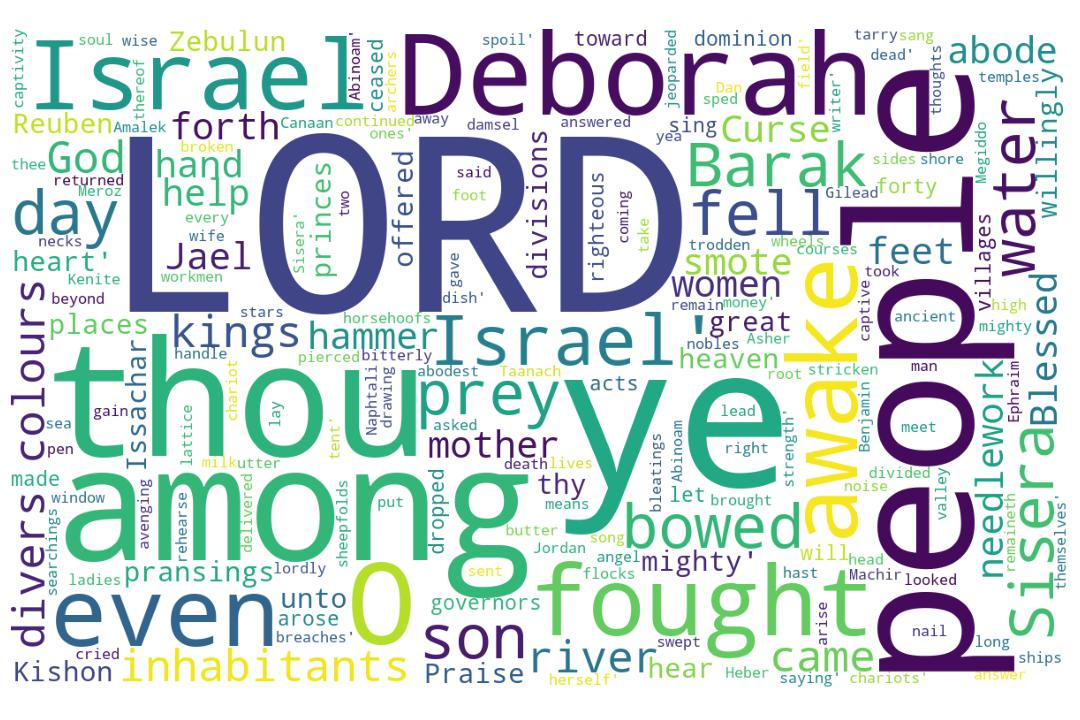
\includegraphics[width=\linewidth]{07OT-Judges/Judges5-WordCloud.jpg}
  \caption{Judges 5 Word Cloud}
  \label{fig:Judges 5 Word Cloud}
\end{figure}


\marginpar{\scriptsize \centering \fcolorbox{bone}{lime}{\textbf{A VICTORY SONG}}\\ (Judges 5) \begin{compactenum}[I.][8]
     \item   The  \textbf{March}  \index[scripture]{Judges!Jdg 05:04} (Jdg 5:4) 
    \item   The  \textbf{Mountains}  \index[scripture]{Judges!Jdg 05:05} (Jdg 5:5) 
    \item   The  \textbf{Melting}  \index[scripture]{Judges!Jdg 05:05} (Jdg 5:5) 
    \item   A  \textbf{Mother}  \index[scripture]{Judges!Jdg 05:07} (Jdg 5:7) 
    \item    \textbf{Mighty Ones}  \index[scripture]{Judges!Jdg 05:13} \index[scripture]{Judges!Jdg 05:22} \index[scripture]{Judges!Jdg 05:23} (Jdg 5:13, 22, 23) 
    \item    \textbf{Megiddo}  \index[scripture]{Judges!Jdg 05:19} (Jdg 5:19) 
    \item   The  \textbf{Dominion}  \index[scripture]{Judges!Jdg 05:13} (Jdg 5:13) 
\end{compactenum}}



\footnote{\textcolor[rgb]{0.00,0.25,0.00}{\hyperlink{JudgesTOC}{Return to end of Table of Contents.}}}\footnote{\href{https://audiobible.com/bible/judges_5.html}{\textcolor[cmyk]{0.99998,1,0,0}{Judges 5 Audio}}}\textcolor[cmyk]{0.99998,1,0,0}{Then sang Deborah and Barak the son of Abinoam on that day, saying,}
[2] \textcolor[cmyk]{0.99998,1,0,0}{Praise ye the LORD for the avenging of Israel, when the people willingly offered themselves.}
[3] \textcolor[cmyk]{0.99998,1,0,0}{Hear, O ye kings; give ear, O ye princes; I, \emph{even} I, will sing unto the LORD; I will sing \emph{praise} to the LORD God of Israel.}
[4] \textcolor[cmyk]{0.99998,1,0,0}{LORD, when thou wentest out of Seir, when thou marchedst out of the field of Edom, the earth trembled, and the heavens dropped, the clouds also dropped water.}
[5] \textcolor[cmyk]{0.99998,1,0,0}{The mountains melted from before the LORD, \emph{even} that Sinai from before the LORD God of Israel.}
[6] \textcolor[cmyk]{0.99998,1,0,0}{In the days of Shamgar the son of Anath, in the days of Jael, the highways were unoccupied, and the travellers walked through byways.}
[7] \textcolor[cmyk]{0.99998,1,0,0}{\emph{The} \emph{inhabitants} \emph{of} the villages ceased, they ceased in Israel, until that I Deborah arose, that I arose a mother in Israel.}
[8] \textcolor[cmyk]{0.99998,1,0,0}{They chose new gods; then \emph{was} war in the gates: was there a shield or spear seen among forty thousand in Israel?}
[9] \textcolor[cmyk]{0.99998,1,0,0}{My heart \emph{is} toward the governors of Israel, that offered themselves willingly among the people. Bless ye the LORD.}
[10] \textcolor[cmyk]{0.99998,1,0,0}{Speak, ye that ride on white asses, ye that sit in judgment, and walk by the way.}
[11] \textcolor[cmyk]{0.99998,1,0,0}{\emph{They} \emph{that} \emph{are} \emph{delivered} from the noise of archers in the places of drawing water, there shall they rehearse the righteous acts of the LORD, \emph{even} the righteous acts \emph{toward} \emph{the} \emph{inhabitants} of his villages in Israel: then shall the people of the LORD go down to the gates.}
[12] \textcolor[cmyk]{0.99998,1,0,0}{Awake, awake, Deborah: awake, awake, utter a song: arise, Barak, and lead thy captivity captive, thou son of Abinoam.}
[13] \textcolor[cmyk]{0.99998,1,0,0}{Then he made him that remaineth have dominion over the nobles among the people: the LORD made me have dominion over the mighty.}
[14] \textcolor[cmyk]{0.99998,1,0,0}{Out of Ephraim \emph{was} \emph{there} a root of them against Amalek; after thee, Benjamin, among thy people; out of Machir came down governors, and out of Zebulun they that handle the pen of the writer.}
[15] \textcolor[cmyk]{0.99998,1,0,0}{And the princes of Issachar \emph{were} with Deborah; even Issachar, and also Barak: he was sent on foot into the valley. For the divisions of Reuben \emph{there} \emph{were} great thoughts of heart.}
[16] \textcolor[cmyk]{0.99998,1,0,0}{Why abodest thou among the sheepfolds, to hear the bleatings of the flocks? For the divisions of Reuben \emph{there} \emph{were} great searchings of heart.}
[17] \textcolor[cmyk]{0.99998,1,0,0}{Gilead abode beyond Jordan: and why did Dan remain in ships? Asher continued on the sea shore, and abode in his breaches.}
[18] \textcolor[cmyk]{0.99998,1,0,0}{Zebulun and Naphtali \emph{were} a people \emph{that} jeoparded their lives unto the death in the high places of the field.}
[19] \textcolor[cmyk]{0.99998,1,0,0}{The kings came \emph{and} fought, then fought the kings of Canaan in Taanach by the waters of Megiddo; they took no gain of money.}
[20] \textcolor[cmyk]{0.99998,1,0,0}{They fought from heaven; the stars in their courses fought against Sisera.}
[21] \textcolor[cmyk]{0.99998,1,0,0}{The river of Kishon swept them away, that ancient river, the river Kishon. O my soul, thou hast trodden down strength.}
[22] \textcolor[cmyk]{0.99998,1,0,0}{Then were the horsehoofs broken by the means of the pransings, the pransings of their mighty ones.}
[23] \textcolor[cmyk]{0.99998,1,0,0}{Curse ye Meroz, said the angel of the LORD, curse ye bitterly the inhabitants thereof; because they came not to the help of the LORD, to the help of the LORD against the mighty.}
[24] \textcolor[cmyk]{0.99998,1,0,0}{Blessed above women shall Jael the wife of Heber the Kenite be, blessed shall she be above women in the tent.}
[25] \textcolor[cmyk]{0.99998,1,0,0}{He asked water, \emph{and} she gave \emph{him} milk; she brought forth butter in a lordly dish.}
[26] \textcolor[cmyk]{0.99998,1,0,0}{She put her hand to the nail, and her right hand to the workmen's hammer; and with the hammer she smote Sisera, she smote off his head, when she had pierced and stricken through his temples.}
[27] \textcolor[cmyk]{0.99998,1,0,0}{At her feet he bowed, he fell, he lay down: at her feet he bowed, he fell: where he bowed, there he fell down dead.}
[28] \textcolor[cmyk]{0.99998,1,0,0}{The mother of Sisera looked out at a window, and cried through the lattice, Why is his chariot \emph{so} long in coming? why tarry the wheels of his chariots?}
[29] \textcolor[cmyk]{0.99998,1,0,0}{Her wise ladies answered her, yea, she returned answer to herself,}\index[AWIP]{Her!Judges!Jdg 05:029}\index[AWIP]{wise!Judges!Jdg 05:029}\index[AWIP]{ladies!Judges!Jdg 05:029}\index[AWIP]{answered!Judges!Jdg 05:029}\index[AWIP]{her!Judges!Jdg 05:029}\index[AWIP]{yea!Judges!Jdg 05:029}\index[AWIP]{she!Judges!Jdg 05:029}\index[AWIP]{returned!Judges!Jdg 05:029}\index[AWIP]{answer!Judges!Jdg 05:029}\index[AWIP]{to!Judges!Jdg 05:029}\index[AWIP]{herself!Judges!Jdg 05:029}\index[NWIV]{11!Judges!Jdg 05:029}
[30] \textcolor[cmyk]{0.99998,1,0,0}{Have they not sped? have they \emph{not} divided the prey; to every man a damsel \emph{or} two; to Sisera a prey of divers colours, a prey of divers colours of needlework, of divers colours of needlework on both sides, \emph{meet} for the necks of \emph{them} \emph{that} \emph{take} the spoil?}
[31] \textcolor[cmyk]{0.99998,1,0,0}{So let all thine enemies perish, O LORD: but \emph{let} them that love him \emph{be} as the sun when he goeth forth in his might. And the land had rest forty years}
\index[NWIV]{13!Judges!Jud 5:1}\index[AWIP]{Then!Judges!Jud 5:1}\index[AWIP]{sang!Judges!Jud 5:1}\index[AWIP]{Deborah!Judges!Jud 5:1}\index[AWIP]{and!Judges!Jud 5:1}\index[AWIP]{Barak!Judges!Jud 5:1}\index[AWIP]{the!Judges!Jud 5:1}\index[AWIP]{son!Judges!Jud 5:1}\index[AWIP]{of!Judges!Jud 5:1}\index[AWIP]{Abinoam!Judges!Jud 5:1}\index[AWIP]{on!Judges!Jud 5:1}\index[AWIP]{that!Judges!Jud 5:1}\index[AWIP]{day!Judges!Jud 5:1}\index[AWIP]{saying!Judges!Jud 5:1}

\index[NWIV]{15!Judges!Jud 5:2}\index[AWIP]{Praise!Judges!Jud 5:2}\index[AWIP]{ye!Judges!Jud 5:2}\index[AWIP]{the!Judges!Jud 5:2}\index[AWIP]{the!Judges!Jud 5:2 (2)}\index[AWIP]{the!Judges!Jud 5:2 (3)}\index[AWIP]{LORD!Judges!Jud 5:2}\index[AWIP]{for!Judges!Jud 5:2}\index[AWIP]{avenging!Judges!Jud 5:2}\index[AWIP]{of!Judges!Jud 5:2}\index[AWIP]{Israel!Judges!Jud 5:2}\index[AWIP]{when!Judges!Jud 5:2}\index[AWIP]{people!Judges!Jud 5:2}\index[AWIP]{willingly!Judges!Jud 5:2}\index[AWIP]{offered!Judges!Jud 5:2}\index[AWIP]{themselves!Judges!Jud 5:2}

\index[NWIV]{27!Judges!Jud 5:3}\index[AWIP]{Hear!Judges!Jud 5:3}\index[AWIP]{O!Judges!Jud 5:3}\index[AWIP]{O!Judges!Jud 5:3 (2)}\index[AWIP]{ye!Judges!Jud 5:3}\index[AWIP]{ye!Judges!Jud 5:3 (2)}\index[AWIP]{kings!Judges!Jud 5:3}\index[AWIP]{give!Judges!Jud 5:3}\index[AWIP]{ear!Judges!Jud 5:3}\index[AWIP]{princes!Judges!Jud 5:3}\index[AWIP]{I!Judges!Jud 5:3}\index[AWIP]{I!Judges!Jud 5:3 (2)}\index[AWIP]{I!Judges!Jud 5:3 (3)}\index[AWIP]{\emph{even}!Judges!Jud 5:3}\index[AWIP]{will!Judges!Jud 5:3}\index[AWIP]{will!Judges!Jud 5:3 (2)}\index[AWIP]{sing!Judges!Jud 5:3}\index[AWIP]{sing!Judges!Jud 5:3 (2)}\index[AWIP]{unto!Judges!Jud 5:3}\index[AWIP]{the!Judges!Jud 5:3}\index[AWIP]{the!Judges!Jud 5:3 (2)}\index[AWIP]{LORD!Judges!Jud 5:3}\index[AWIP]{LORD!Judges!Jud 5:3 (2)}\index[AWIP]{\emph{praise}!Judges!Jud 5:3}\index[AWIP]{to!Judges!Jud 5:3}\index[AWIP]{God!Judges!Jud 5:3}\index[AWIP]{of!Judges!Jud 5:3}\index[AWIP]{Israel!Judges!Jud 5:3}\index[AWIP]{\emph{even}!Judges!Jud 5:3}\index[AWIP]{\emph{praise}!Judges!Jud 5:3}

\index[NWIV]{28!Judges!Jud 5:4}\index[AWIP]{LORD!Judges!Jud 5:4}\index[AWIP]{when!Judges!Jud 5:4}\index[AWIP]{when!Judges!Jud 5:4 (2)}\index[AWIP]{thou!Judges!Jud 5:4}\index[AWIP]{thou!Judges!Jud 5:4 (2)}\index[AWIP]{wentest!Judges!Jud 5:4}\index[AWIP]{out!Judges!Jud 5:4}\index[AWIP]{out!Judges!Jud 5:4 (2)}\index[AWIP]{of!Judges!Jud 5:4}\index[AWIP]{of!Judges!Jud 5:4 (2)}\index[AWIP]{of!Judges!Jud 5:4 (3)}\index[AWIP]{Seir!Judges!Jud 5:4}\index[AWIP]{marchedst!Judges!Jud 5:4}\index[AWIP]{the!Judges!Jud 5:4}\index[AWIP]{the!Judges!Jud 5:4 (2)}\index[AWIP]{the!Judges!Jud 5:4 (3)}\index[AWIP]{the!Judges!Jud 5:4 (4)}\index[AWIP]{field!Judges!Jud 5:4}\index[AWIP]{Edom!Judges!Jud 5:4}\index[AWIP]{earth!Judges!Jud 5:4}\index[AWIP]{trembled!Judges!Jud 5:4}\index[AWIP]{and!Judges!Jud 5:4}\index[AWIP]{heavens!Judges!Jud 5:4}\index[AWIP]{dropped!Judges!Jud 5:4}\index[AWIP]{dropped!Judges!Jud 5:4 (2)}\index[AWIP]{clouds!Judges!Jud 5:4}\index[AWIP]{also!Judges!Jud 5:4}\index[AWIP]{water!Judges!Jud 5:4}

\index[NWIV]{17!Judges!Jud 5:5}\index[AWIP]{The!Judges!Jud 5:5}\index[AWIP]{mountains!Judges!Jud 5:5}\index[AWIP]{melted!Judges!Jud 5:5}\index[AWIP]{from!Judges!Jud 5:5}\index[AWIP]{from!Judges!Jud 5:5 (2)}\index[AWIP]{before!Judges!Jud 5:5}\index[AWIP]{before!Judges!Jud 5:5 (2)}\index[AWIP]{the!Judges!Jud 5:5}\index[AWIP]{the!Judges!Jud 5:5 (2)}\index[AWIP]{LORD!Judges!Jud 5:5}\index[AWIP]{LORD!Judges!Jud 5:5 (2)}\index[AWIP]{\emph{even}!Judges!Jud 5:5}\index[AWIP]{that!Judges!Jud 5:5}\index[AWIP]{Sinai!Judges!Jud 5:5}\index[AWIP]{God!Judges!Jud 5:5}\index[AWIP]{of!Judges!Jud 5:5}\index[AWIP]{Israel!Judges!Jud 5:5}\index[AWIP]{\emph{even}!Judges!Jud 5:5}

\index[NWIV]{24!Judges!Jud 5:6}\index[AWIP]{In!Judges!Jud 5:6}\index[AWIP]{the!Judges!Jud 5:6}\index[AWIP]{the!Judges!Jud 5:6 (2)}\index[AWIP]{the!Judges!Jud 5:6 (3)}\index[AWIP]{the!Judges!Jud 5:6 (4)}\index[AWIP]{the!Judges!Jud 5:6 (5)}\index[AWIP]{days!Judges!Jud 5:6}\index[AWIP]{days!Judges!Jud 5:6 (2)}\index[AWIP]{of!Judges!Jud 5:6}\index[AWIP]{of!Judges!Jud 5:6 (2)}\index[AWIP]{of!Judges!Jud 5:6 (3)}\index[AWIP]{Shamgar!Judges!Jud 5:6}\index[AWIP]{son!Judges!Jud 5:6}\index[AWIP]{Anath!Judges!Jud 5:6}\index[AWIP]{in!Judges!Jud 5:6}\index[AWIP]{Jael!Judges!Jud 5:6}\index[AWIP]{highways!Judges!Jud 5:6}\index[AWIP]{were!Judges!Jud 5:6}\index[AWIP]{unoccupied!Judges!Jud 5:6}\index[AWIP]{and!Judges!Jud 5:6}\index[AWIP]{travellers!Judges!Jud 5:6}\index[AWIP]{walked!Judges!Jud 5:6}\index[AWIP]{through!Judges!Jud 5:6}\index[AWIP]{byways!Judges!Jud 5:6}

\index[NWIV]{22!Judges!Jud 5:7}\index[AWIP]{\emph{The}!Judges!Jud 5:7}\index[AWIP]{\emph{inhabitants}!Judges!Jud 5:7}\index[AWIP]{\emph{of}!Judges!Jud 5:7}\index[AWIP]{the!Judges!Jud 5:7}\index[AWIP]{villages!Judges!Jud 5:7}\index[AWIP]{ceased!Judges!Jud 5:7}\index[AWIP]{ceased!Judges!Jud 5:7 (2)}\index[AWIP]{they!Judges!Jud 5:7}\index[AWIP]{in!Judges!Jud 5:7}\index[AWIP]{in!Judges!Jud 5:7 (2)}\index[AWIP]{Israel!Judges!Jud 5:7}\index[AWIP]{Israel!Judges!Jud 5:7 (2)}\index[AWIP]{until!Judges!Jud 5:7}\index[AWIP]{that!Judges!Jud 5:7}\index[AWIP]{that!Judges!Jud 5:7 (2)}\index[AWIP]{I!Judges!Jud 5:7}\index[AWIP]{I!Judges!Jud 5:7 (2)}\index[AWIP]{Deborah!Judges!Jud 5:7}\index[AWIP]{arose!Judges!Jud 5:7}\index[AWIP]{arose!Judges!Jud 5:7 (2)}\index[AWIP]{a!Judges!Jud 5:7}\index[AWIP]{mother!Judges!Jud 5:7}\index[AWIP]{\emph{The}!Judges!Jud 5:7}\index[AWIP]{\emph{inhabitants}!Judges!Jud 5:7}\index[AWIP]{\emph{of}!Judges!Jud 5:7}

\index[NWIV]{22!Judges!Jud 5:8}\index[AWIP]{They!Judges!Jud 5:8}\index[AWIP]{chose!Judges!Jud 5:8}\index[AWIP]{new!Judges!Jud 5:8}\index[AWIP]{gods!Judges!Jud 5:8}\index[AWIP]{then!Judges!Jud 5:8}\index[AWIP]{\emph{was}!Judges!Jud 5:8}\index[AWIP]{war!Judges!Jud 5:8}\index[AWIP]{in!Judges!Jud 5:8}\index[AWIP]{in!Judges!Jud 5:8 (2)}\index[AWIP]{the!Judges!Jud 5:8}\index[AWIP]{gates!Judges!Jud 5:8}\index[AWIP]{was!Judges!Jud 5:8}\index[AWIP]{there!Judges!Jud 5:8}\index[AWIP]{a!Judges!Jud 5:8}\index[AWIP]{shield!Judges!Jud 5:8}\index[AWIP]{or!Judges!Jud 5:8}\index[AWIP]{spear!Judges!Jud 5:8}\index[AWIP]{seen!Judges!Jud 5:8}\index[AWIP]{among!Judges!Jud 5:8}\index[AWIP]{forty!Judges!Jud 5:8}\index[AWIP]{thousand!Judges!Jud 5:8}\index[AWIP]{Israel?!Judges!Jud 5:8}\index[AWIP]{\emph{was}!Judges!Jud 5:8}

\index[NWIV]{19!Judges!Jud 5:9}\index[AWIP]{My!Judges!Jud 5:9}\index[AWIP]{heart!Judges!Jud 5:9}\index[AWIP]{\emph{is}!Judges!Jud 5:9}\index[AWIP]{toward!Judges!Jud 5:9}\index[AWIP]{the!Judges!Jud 5:9}\index[AWIP]{the!Judges!Jud 5:9 (2)}\index[AWIP]{the!Judges!Jud 5:9 (3)}\index[AWIP]{governors!Judges!Jud 5:9}\index[AWIP]{of!Judges!Jud 5:9}\index[AWIP]{Israel!Judges!Jud 5:9}\index[AWIP]{that!Judges!Jud 5:9}\index[AWIP]{offered!Judges!Jud 5:9}\index[AWIP]{themselves!Judges!Jud 5:9}\index[AWIP]{willingly!Judges!Jud 5:9}\index[AWIP]{among!Judges!Jud 5:9}\index[AWIP]{people!Judges!Jud 5:9}\index[AWIP]{Bless!Judges!Jud 5:9}\index[AWIP]{ye!Judges!Jud 5:9}\index[AWIP]{LORD!Judges!Jud 5:9}\index[AWIP]{\emph{is}!Judges!Jud 5:9}

\index[NWIV]{17!Judges!Jud 5:10}\index[AWIP]{Speak!Judges!Jud 5:10}\index[AWIP]{ye!Judges!Jud 5:10}\index[AWIP]{ye!Judges!Jud 5:10 (2)}\index[AWIP]{that!Judges!Jud 5:10}\index[AWIP]{that!Judges!Jud 5:10 (2)}\index[AWIP]{ride!Judges!Jud 5:10}\index[AWIP]{on!Judges!Jud 5:10}\index[AWIP]{white!Judges!Jud 5:10}\index[AWIP]{asses!Judges!Jud 5:10}\index[AWIP]{sit!Judges!Jud 5:10}\index[AWIP]{in!Judges!Jud 5:10}\index[AWIP]{judgment!Judges!Jud 5:10}\index[AWIP]{and!Judges!Jud 5:10}\index[AWIP]{walk!Judges!Jud 5:10}\index[AWIP]{by!Judges!Jud 5:10}\index[AWIP]{the!Judges!Jud 5:10}\index[AWIP]{way!Judges!Jud 5:10}

\index[NWIV]{49!Judges!Jud 5:11}\index[AWIP]{\emph{They}!Judges!Jud 5:11}\index[AWIP]{\emph{that}!Judges!Jud 5:11}\index[AWIP]{\emph{are}!Judges!Jud 5:11}\index[AWIP]{\emph{delivered}!Judges!Jud 5:11}\index[AWIP]{from!Judges!Jud 5:11}\index[AWIP]{the!Judges!Jud 5:11}\index[AWIP]{the!Judges!Jud 5:11 (2)}\index[AWIP]{the!Judges!Jud 5:11 (3)}\index[AWIP]{the!Judges!Jud 5:11 (4)}\index[AWIP]{the!Judges!Jud 5:11 (5)}\index[AWIP]{the!Judges!Jud 5:11 (6)}\index[AWIP]{the!Judges!Jud 5:11 (7)}\index[AWIP]{the!Judges!Jud 5:11 (8)}\index[AWIP]{noise!Judges!Jud 5:11}\index[AWIP]{of!Judges!Jud 5:11}\index[AWIP]{of!Judges!Jud 5:11 (2)}\index[AWIP]{of!Judges!Jud 5:11 (3)}\index[AWIP]{of!Judges!Jud 5:11 (4)}\index[AWIP]{of!Judges!Jud 5:11 (5)}\index[AWIP]{archers!Judges!Jud 5:11}\index[AWIP]{in!Judges!Jud 5:11}\index[AWIP]{in!Judges!Jud 5:11 (2)}\index[AWIP]{places!Judges!Jud 5:11}\index[AWIP]{drawing!Judges!Jud 5:11}\index[AWIP]{water!Judges!Jud 5:11}\index[AWIP]{there!Judges!Jud 5:11}\index[AWIP]{shall!Judges!Jud 5:11}\index[AWIP]{shall!Judges!Jud 5:11 (2)}\index[AWIP]{they!Judges!Jud 5:11}\index[AWIP]{rehearse!Judges!Jud 5:11}\index[AWIP]{righteous!Judges!Jud 5:11}\index[AWIP]{righteous!Judges!Jud 5:11 (2)}\index[AWIP]{acts!Judges!Jud 5:11}\index[AWIP]{acts!Judges!Jud 5:11 (2)}\index[AWIP]{LORD!Judges!Jud 5:11}\index[AWIP]{LORD!Judges!Jud 5:11 (2)}\index[AWIP]{\emph{even}!Judges!Jud 5:11}\index[AWIP]{\emph{toward}!Judges!Jud 5:11}\index[AWIP]{\emph{the}!Judges!Jud 5:11}\index[AWIP]{\emph{inhabitants}!Judges!Jud 5:11}\index[AWIP]{his!Judges!Jud 5:11}\index[AWIP]{villages!Judges!Jud 5:11}\index[AWIP]{Israel!Judges!Jud 5:11}\index[AWIP]{then!Judges!Jud 5:11}\index[AWIP]{people!Judges!Jud 5:11}\index[AWIP]{go!Judges!Jud 5:11}\index[AWIP]{down!Judges!Jud 5:11}\index[AWIP]{to!Judges!Jud 5:11}\index[AWIP]{gates!Judges!Jud 5:11}\index[AWIP]{\emph{They}!Judges!Jud 5:11}\index[AWIP]{\emph{that}!Judges!Jud 5:11}\index[AWIP]{\emph{are}!Judges!Jud 5:11}\index[AWIP]{\emph{delivered}!Judges!Jud 5:11}\index[AWIP]{\emph{even}!Judges!Jud 5:11}\index[AWIP]{\emph{toward}!Judges!Jud 5:11}\index[AWIP]{\emph{the}!Judges!Jud 5:11}\index[AWIP]{\emph{inhabitants}!Judges!Jud 5:11}

\index[NWIV]{19!Judges!Jud 5:12}\index[AWIP]{Awake!Judges!Jud 5:12}\index[AWIP]{awake!Judges!Jud 5:12}\index[AWIP]{awake!Judges!Jud 5:12 (2)}\index[AWIP]{awake!Judges!Jud 5:12 (3)}\index[AWIP]{Deborah!Judges!Jud 5:12}\index[AWIP]{utter!Judges!Jud 5:12}\index[AWIP]{a!Judges!Jud 5:12}\index[AWIP]{song!Judges!Jud 5:12}\index[AWIP]{arise!Judges!Jud 5:12}\index[AWIP]{Barak!Judges!Jud 5:12}\index[AWIP]{and!Judges!Jud 5:12}\index[AWIP]{lead!Judges!Jud 5:12}\index[AWIP]{thy!Judges!Jud 5:12}\index[AWIP]{captivity!Judges!Jud 5:12}\index[AWIP]{captive!Judges!Jud 5:12}\index[AWIP]{thou!Judges!Jud 5:12}\index[AWIP]{son!Judges!Jud 5:12}\index[AWIP]{of!Judges!Jud 5:12}\index[AWIP]{Abinoam!Judges!Jud 5:12}

\index[NWIV]{23!Judges!Jud 5:13}\index[AWIP]{Then!Judges!Jud 5:13}\index[AWIP]{he!Judges!Jud 5:13}\index[AWIP]{made!Judges!Jud 5:13}\index[AWIP]{made!Judges!Jud 5:13 (2)}\index[AWIP]{him!Judges!Jud 5:13}\index[AWIP]{that!Judges!Jud 5:13}\index[AWIP]{remaineth!Judges!Jud 5:13}\index[AWIP]{have!Judges!Jud 5:13}\index[AWIP]{have!Judges!Jud 5:13 (2)}\index[AWIP]{dominion!Judges!Jud 5:13}\index[AWIP]{dominion!Judges!Jud 5:13 (2)}\index[AWIP]{over!Judges!Jud 5:13}\index[AWIP]{over!Judges!Jud 5:13 (2)}\index[AWIP]{the!Judges!Jud 5:13}\index[AWIP]{the!Judges!Jud 5:13 (2)}\index[AWIP]{the!Judges!Jud 5:13 (3)}\index[AWIP]{the!Judges!Jud 5:13 (4)}\index[AWIP]{nobles!Judges!Jud 5:13}\index[AWIP]{among!Judges!Jud 5:13}\index[AWIP]{people!Judges!Jud 5:13}\index[AWIP]{LORD!Judges!Jud 5:13}\index[AWIP]{me!Judges!Jud 5:13}\index[AWIP]{mighty!Judges!Jud 5:13}

\index[NWIV]{35!Judges!Jud 5:14}\index[AWIP]{Out!Judges!Jud 5:14}\index[AWIP]{of!Judges!Jud 5:14}\index[AWIP]{of!Judges!Jud 5:14 (2)}\index[AWIP]{of!Judges!Jud 5:14 (3)}\index[AWIP]{of!Judges!Jud 5:14 (4)}\index[AWIP]{of!Judges!Jud 5:14 (5)}\index[AWIP]{Ephraim!Judges!Jud 5:14}\index[AWIP]{\emph{was}!Judges!Jud 5:14}\index[AWIP]{\emph{there}!Judges!Jud 5:14}\index[AWIP]{a!Judges!Jud 5:14}\index[AWIP]{root!Judges!Jud 5:14}\index[AWIP]{them!Judges!Jud 5:14}\index[AWIP]{against!Judges!Jud 5:14}\index[AWIP]{Amalek!Judges!Jud 5:14}\index[AWIP]{after!Judges!Jud 5:14}\index[AWIP]{thee!Judges!Jud 5:14}\index[AWIP]{Benjamin!Judges!Jud 5:14}\index[AWIP]{among!Judges!Jud 5:14}\index[AWIP]{thy!Judges!Jud 5:14}\index[AWIP]{people!Judges!Jud 5:14}\index[AWIP]{out!Judges!Jud 5:14}\index[AWIP]{out!Judges!Jud 5:14 (2)}\index[AWIP]{Machir!Judges!Jud 5:14}\index[AWIP]{came!Judges!Jud 5:14}\index[AWIP]{down!Judges!Jud 5:14}\index[AWIP]{governors!Judges!Jud 5:14}\index[AWIP]{and!Judges!Jud 5:14}\index[AWIP]{Zebulun!Judges!Jud 5:14}\index[AWIP]{they!Judges!Jud 5:14}\index[AWIP]{that!Judges!Jud 5:14}\index[AWIP]{handle!Judges!Jud 5:14}\index[AWIP]{the!Judges!Jud 5:14}\index[AWIP]{the!Judges!Jud 5:14 (2)}\index[AWIP]{pen!Judges!Jud 5:14}\index[AWIP]{writer!Judges!Jud 5:14}\index[AWIP]{\emph{was}!Judges!Jud 5:14}\index[AWIP]{\emph{there}!Judges!Jud 5:14}

\index[NWIV]{32!Judges!Jud 5:15}\index[AWIP]{And!Judges!Jud 5:15}\index[AWIP]{the!Judges!Jud 5:15}\index[AWIP]{the!Judges!Jud 5:15 (2)}\index[AWIP]{the!Judges!Jud 5:15 (3)}\index[AWIP]{princes!Judges!Jud 5:15}\index[AWIP]{of!Judges!Jud 5:15}\index[AWIP]{of!Judges!Jud 5:15 (2)}\index[AWIP]{of!Judges!Jud 5:15 (3)}\index[AWIP]{Issachar!Judges!Jud 5:15}\index[AWIP]{Issachar!Judges!Jud 5:15 (2)}\index[AWIP]{\emph{were}!Judges!Jud 5:15}\index[AWIP]{\emph{were}!Judges!Jud 5:15 (2)}\index[AWIP]{with!Judges!Jud 5:15}\index[AWIP]{Deborah!Judges!Jud 5:15}\index[AWIP]{even!Judges!Jud 5:15}\index[AWIP]{and!Judges!Jud 5:15}\index[AWIP]{also!Judges!Jud 5:15}\index[AWIP]{Barak!Judges!Jud 5:15}\index[AWIP]{he!Judges!Jud 5:15}\index[AWIP]{was!Judges!Jud 5:15}\index[AWIP]{sent!Judges!Jud 5:15}\index[AWIP]{on!Judges!Jud 5:15}\index[AWIP]{foot!Judges!Jud 5:15}\index[AWIP]{into!Judges!Jud 5:15}\index[AWIP]{valley!Judges!Jud 5:15}\index[AWIP]{For!Judges!Jud 5:15}\index[AWIP]{divisions!Judges!Jud 5:15}\index[AWIP]{Reuben!Judges!Jud 5:15}\index[AWIP]{\emph{there}!Judges!Jud 5:15}\index[AWIP]{great!Judges!Jud 5:15}\index[AWIP]{thoughts!Judges!Jud 5:15}\index[AWIP]{heart!Judges!Jud 5:15}\index[AWIP]{\emph{were}!Judges!Jud 5:15}\index[AWIP]{\emph{were}!Judges!Jud 5:15 (2)}\index[AWIP]{\emph{there}!Judges!Jud 5:15}

\index[NWIV]{24!Judges!Jud 5:16}\index[AWIP]{Why!Judges!Jud 5:16}\index[AWIP]{abodest!Judges!Jud 5:16}\index[AWIP]{thou!Judges!Jud 5:16}\index[AWIP]{among!Judges!Jud 5:16}\index[AWIP]{the!Judges!Jud 5:16}\index[AWIP]{the!Judges!Jud 5:16 (2)}\index[AWIP]{the!Judges!Jud 5:16 (3)}\index[AWIP]{the!Judges!Jud 5:16 (4)}\index[AWIP]{sheepfolds!Judges!Jud 5:16}\index[AWIP]{to!Judges!Jud 5:16}\index[AWIP]{hear!Judges!Jud 5:16}\index[AWIP]{bleatings!Judges!Jud 5:16}\index[AWIP]{of!Judges!Jud 5:16}\index[AWIP]{of!Judges!Jud 5:16 (2)}\index[AWIP]{of!Judges!Jud 5:16 (3)}\index[AWIP]{flocks?!Judges!Jud 5:16}\index[AWIP]{For!Judges!Jud 5:16}\index[AWIP]{divisions!Judges!Jud 5:16}\index[AWIP]{Reuben!Judges!Jud 5:16}\index[AWIP]{\emph{there}!Judges!Jud 5:16}\index[AWIP]{\emph{were}!Judges!Jud 5:16}\index[AWIP]{great!Judges!Jud 5:16}\index[AWIP]{searchings!Judges!Jud 5:16}\index[AWIP]{heart!Judges!Jud 5:16}\index[AWIP]{\emph{there}!Judges!Jud 5:16}\index[AWIP]{\emph{were}!Judges!Jud 5:16}

\index[NWIV]{22!Judges!Jud 5:17}\index[AWIP]{Gilead!Judges!Jud 5:17}\index[AWIP]{abode!Judges!Jud 5:17}\index[AWIP]{abode!Judges!Jud 5:17 (2)}\index[AWIP]{beyond!Judges!Jud 5:17}\index[AWIP]{Jordan!Judges!Jud 5:17}\index[AWIP]{and!Judges!Jud 5:17}\index[AWIP]{and!Judges!Jud 5:17 (2)}\index[AWIP]{why!Judges!Jud 5:17}\index[AWIP]{did!Judges!Jud 5:17}\index[AWIP]{Dan!Judges!Jud 5:17}\index[AWIP]{remain!Judges!Jud 5:17}\index[AWIP]{in!Judges!Jud 5:17}\index[AWIP]{in!Judges!Jud 5:17 (2)}\index[AWIP]{ships?!Judges!Jud 5:17}\index[AWIP]{Asher!Judges!Jud 5:17}\index[AWIP]{continued!Judges!Jud 5:17}\index[AWIP]{on!Judges!Jud 5:17}\index[AWIP]{the!Judges!Jud 5:17}\index[AWIP]{sea!Judges!Jud 5:17}\index[AWIP]{shore!Judges!Jud 5:17}\index[AWIP]{his!Judges!Jud 5:17}\index[AWIP]{breaches!Judges!Jud 5:17}

\index[NWIV]{20!Judges!Jud 5:18}\index[AWIP]{Zebulun!Judges!Jud 5:18}\index[AWIP]{and!Judges!Jud 5:18}\index[AWIP]{Naphtali!Judges!Jud 5:18}\index[AWIP]{\emph{were}!Judges!Jud 5:18}\index[AWIP]{a!Judges!Jud 5:18}\index[AWIP]{people!Judges!Jud 5:18}\index[AWIP]{\emph{that}!Judges!Jud 5:18}\index[AWIP]{jeoparded!Judges!Jud 5:18}\index[AWIP]{their!Judges!Jud 5:18}\index[AWIP]{lives!Judges!Jud 5:18}\index[AWIP]{unto!Judges!Jud 5:18}\index[AWIP]{the!Judges!Jud 5:18}\index[AWIP]{the!Judges!Jud 5:18 (2)}\index[AWIP]{the!Judges!Jud 5:18 (3)}\index[AWIP]{death!Judges!Jud 5:18}\index[AWIP]{in!Judges!Jud 5:18}\index[AWIP]{high!Judges!Jud 5:18}\index[AWIP]{places!Judges!Jud 5:18}\index[AWIP]{of!Judges!Jud 5:18}\index[AWIP]{field!Judges!Jud 5:18}\index[AWIP]{\emph{were}!Judges!Jud 5:18}\index[AWIP]{\emph{that}!Judges!Jud 5:18}

\index[NWIV]{24!Judges!Jud 5:19}\index[AWIP]{The!Judges!Jud 5:19}\index[AWIP]{kings!Judges!Jud 5:19}\index[AWIP]{kings!Judges!Jud 5:19 (2)}\index[AWIP]{came!Judges!Jud 5:19}\index[AWIP]{\emph{and}!Judges!Jud 5:19}\index[AWIP]{fought!Judges!Jud 5:19}\index[AWIP]{fought!Judges!Jud 5:19 (2)}\index[AWIP]{then!Judges!Jud 5:19}\index[AWIP]{the!Judges!Jud 5:19}\index[AWIP]{the!Judges!Jud 5:19 (2)}\index[AWIP]{of!Judges!Jud 5:19}\index[AWIP]{of!Judges!Jud 5:19 (2)}\index[AWIP]{of!Judges!Jud 5:19 (3)}\index[AWIP]{Canaan!Judges!Jud 5:19}\index[AWIP]{in!Judges!Jud 5:19}\index[AWIP]{Taanach!Judges!Jud 5:19}\index[AWIP]{by!Judges!Jud 5:19}\index[AWIP]{waters!Judges!Jud 5:19}\index[AWIP]{Megiddo!Judges!Jud 5:19}\index[AWIP]{they!Judges!Jud 5:19}\index[AWIP]{took!Judges!Jud 5:19}\index[AWIP]{no!Judges!Jud 5:19}\index[AWIP]{gain!Judges!Jud 5:19}\index[AWIP]{money!Judges!Jud 5:19}\index[AWIP]{\emph{and}!Judges!Jud 5:19}

\index[NWIV]{12!Judges!Jud 5:20}\index[AWIP]{They!Judges!Jud 5:20}\index[AWIP]{fought!Judges!Jud 5:20}\index[AWIP]{fought!Judges!Jud 5:20 (2)}\index[AWIP]{from!Judges!Jud 5:20}\index[AWIP]{heaven!Judges!Jud 5:20}\index[AWIP]{the!Judges!Jud 5:20}\index[AWIP]{stars!Judges!Jud 5:20}\index[AWIP]{in!Judges!Jud 5:20}\index[AWIP]{their!Judges!Jud 5:20}\index[AWIP]{courses!Judges!Jud 5:20}\index[AWIP]{against!Judges!Jud 5:20}\index[AWIP]{Sisera!Judges!Jud 5:20}

\index[NWIV]{21!Judges!Jud 5:21}\index[AWIP]{The!Judges!Jud 5:21}\index[AWIP]{river!Judges!Jud 5:21}\index[AWIP]{river!Judges!Jud 5:21 (2)}\index[AWIP]{river!Judges!Jud 5:21 (3)}\index[AWIP]{of!Judges!Jud 5:21}\index[AWIP]{Kishon!Judges!Jud 5:21}\index[AWIP]{Kishon!Judges!Jud 5:21 (2)}\index[AWIP]{swept!Judges!Jud 5:21}\index[AWIP]{them!Judges!Jud 5:21}\index[AWIP]{away!Judges!Jud 5:21}\index[AWIP]{that!Judges!Jud 5:21}\index[AWIP]{ancient!Judges!Jud 5:21}\index[AWIP]{the!Judges!Jud 5:21}\index[AWIP]{O!Judges!Jud 5:21}\index[AWIP]{my!Judges!Jud 5:21}\index[AWIP]{soul!Judges!Jud 5:21}\index[AWIP]{thou!Judges!Jud 5:21}\index[AWIP]{hast!Judges!Jud 5:21}\index[AWIP]{trodden!Judges!Jud 5:21}\index[AWIP]{down!Judges!Jud 5:21}\index[AWIP]{strength!Judges!Jud 5:21}

\index[NWIV]{17!Judges!Jud 5:22}\index[AWIP]{Then!Judges!Jud 5:22}\index[AWIP]{were!Judges!Jud 5:22}\index[AWIP]{the!Judges!Jud 5:22}\index[AWIP]{the!Judges!Jud 5:22 (2)}\index[AWIP]{the!Judges!Jud 5:22 (3)}\index[AWIP]{the!Judges!Jud 5:22 (4)}\index[AWIP]{horsehoofs!Judges!Jud 5:22}\index[AWIP]{broken!Judges!Jud 5:22}\index[AWIP]{by!Judges!Jud 5:22}\index[AWIP]{means!Judges!Jud 5:22}\index[AWIP]{of!Judges!Jud 5:22}\index[AWIP]{of!Judges!Jud 5:22 (2)}\index[AWIP]{pransings!Judges!Jud 5:22}\index[AWIP]{pransings!Judges!Jud 5:22 (2)}\index[AWIP]{their!Judges!Jud 5:22}\index[AWIP]{mighty!Judges!Jud 5:22}\index[AWIP]{ones!Judges!Jud 5:22}

\index[NWIV]{34!Judges!Jud 5:23}\index[AWIP]{Curse!Judges!Jud 5:23}\index[AWIP]{ye!Judges!Jud 5:23}\index[AWIP]{ye!Judges!Jud 5:23 (2)}\index[AWIP]{Meroz!Judges!Jud 5:23}\index[AWIP]{said!Judges!Jud 5:23}\index[AWIP]{the!Judges!Jud 5:23}\index[AWIP]{the!Judges!Jud 5:23 (2)}\index[AWIP]{the!Judges!Jud 5:23 (3)}\index[AWIP]{the!Judges!Jud 5:23 (4)}\index[AWIP]{the!Judges!Jud 5:23 (5)}\index[AWIP]{the!Judges!Jud 5:23 (6)}\index[AWIP]{the!Judges!Jud 5:23 (7)}\index[AWIP]{the!Judges!Jud 5:23 (8)}\index[AWIP]{angel!Judges!Jud 5:23}\index[AWIP]{of!Judges!Jud 5:23}\index[AWIP]{of!Judges!Jud 5:23 (2)}\index[AWIP]{of!Judges!Jud 5:23 (3)}\index[AWIP]{LORD!Judges!Jud 5:23}\index[AWIP]{LORD!Judges!Jud 5:23 (2)}\index[AWIP]{LORD!Judges!Jud 5:23 (3)}\index[AWIP]{curse!Judges!Jud 5:23}\index[AWIP]{bitterly!Judges!Jud 5:23}\index[AWIP]{inhabitants!Judges!Jud 5:23}\index[AWIP]{thereof!Judges!Jud 5:23}\index[AWIP]{because!Judges!Jud 5:23}\index[AWIP]{they!Judges!Jud 5:23}\index[AWIP]{came!Judges!Jud 5:23}\index[AWIP]{not!Judges!Jud 5:23}\index[AWIP]{to!Judges!Jud 5:23}\index[AWIP]{to!Judges!Jud 5:23 (2)}\index[AWIP]{help!Judges!Jud 5:23}\index[AWIP]{help!Judges!Jud 5:23 (2)}\index[AWIP]{against!Judges!Jud 5:23}\index[AWIP]{mighty!Judges!Jud 5:23}

\index[NWIV]{21!Judges!Jud 5:24}\index[AWIP]{Blessed!Judges!Jud 5:24}\index[AWIP]{above!Judges!Jud 5:24}\index[AWIP]{above!Judges!Jud 5:24 (2)}\index[AWIP]{women!Judges!Jud 5:24}\index[AWIP]{women!Judges!Jud 5:24 (2)}\index[AWIP]{shall!Judges!Jud 5:24}\index[AWIP]{shall!Judges!Jud 5:24 (2)}\index[AWIP]{Jael!Judges!Jud 5:24}\index[AWIP]{the!Judges!Jud 5:24}\index[AWIP]{the!Judges!Jud 5:24 (2)}\index[AWIP]{the!Judges!Jud 5:24 (3)}\index[AWIP]{wife!Judges!Jud 5:24}\index[AWIP]{of!Judges!Jud 5:24}\index[AWIP]{Heber!Judges!Jud 5:24}\index[AWIP]{Kenite!Judges!Jud 5:24}\index[AWIP]{be!Judges!Jud 5:24}\index[AWIP]{be!Judges!Jud 5:24 (2)}\index[AWIP]{blessed!Judges!Jud 5:24}\index[AWIP]{she!Judges!Jud 5:24}\index[AWIP]{in!Judges!Jud 5:24}\index[AWIP]{tent!Judges!Jud 5:24}

\index[NWIV]{16!Judges!Jud 5:25}\index[AWIP]{He!Judges!Jud 5:25}\index[AWIP]{asked!Judges!Jud 5:25}\index[AWIP]{water!Judges!Jud 5:25}\index[AWIP]{\emph{and}!Judges!Jud 5:25}\index[AWIP]{she!Judges!Jud 5:25}\index[AWIP]{she!Judges!Jud 5:25 (2)}\index[AWIP]{gave!Judges!Jud 5:25}\index[AWIP]{\emph{him}!Judges!Jud 5:25}\index[AWIP]{milk!Judges!Jud 5:25}\index[AWIP]{brought!Judges!Jud 5:25}\index[AWIP]{forth!Judges!Jud 5:25}\index[AWIP]{butter!Judges!Jud 5:25}\index[AWIP]{in!Judges!Jud 5:25}\index[AWIP]{a!Judges!Jud 5:25}\index[AWIP]{lordly!Judges!Jud 5:25}\index[AWIP]{dish!Judges!Jud 5:25}\index[AWIP]{\emph{and}!Judges!Jud 5:25}\index[AWIP]{\emph{him}!Judges!Jud 5:25}

\index[NWIV]{36!Judges!Jud 5:26}\index[AWIP]{She!Judges!Jud 5:26}\index[AWIP]{put!Judges!Jud 5:26}\index[AWIP]{her!Judges!Jud 5:26}\index[AWIP]{her!Judges!Jud 5:26 (2)}\index[AWIP]{hand!Judges!Jud 5:26}\index[AWIP]{hand!Judges!Jud 5:26 (2)}\index[AWIP]{to!Judges!Jud 5:26}\index[AWIP]{to!Judges!Jud 5:26 (2)}\index[AWIP]{the!Judges!Jud 5:26}\index[AWIP]{the!Judges!Jud 5:26 (2)}\index[AWIP]{the!Judges!Jud 5:26 (3)}\index[AWIP]{nail!Judges!Jud 5:26}\index[AWIP]{and!Judges!Jud 5:26}\index[AWIP]{and!Judges!Jud 5:26 (2)}\index[AWIP]{and!Judges!Jud 5:26 (3)}\index[AWIP]{right!Judges!Jud 5:26}\index[AWIP]{workmen's!Judges!Jud 5:26}\index[AWIP]{hammer!Judges!Jud 5:26}\index[AWIP]{hammer!Judges!Jud 5:26 (2)}\index[AWIP]{with!Judges!Jud 5:26}\index[AWIP]{she!Judges!Jud 5:26}\index[AWIP]{she!Judges!Jud 5:26 (2)}\index[AWIP]{she!Judges!Jud 5:26 (3)}\index[AWIP]{smote!Judges!Jud 5:26}\index[AWIP]{smote!Judges!Jud 5:26 (2)}\index[AWIP]{Sisera!Judges!Jud 5:26}\index[AWIP]{off!Judges!Jud 5:26}\index[AWIP]{his!Judges!Jud 5:26}\index[AWIP]{his!Judges!Jud 5:26 (2)}\index[AWIP]{head!Judges!Jud 5:26}\index[AWIP]{when!Judges!Jud 5:26}\index[AWIP]{had!Judges!Jud 5:26}\index[AWIP]{pierced!Judges!Jud 5:26}\index[AWIP]{stricken!Judges!Jud 5:26}\index[AWIP]{through!Judges!Jud 5:26}\index[AWIP]{temples!Judges!Jud 5:26}

\index[NWIV]{25!Judges!Jud 5:27}\index[AWIP]{At!Judges!Jud 5:27}\index[AWIP]{her!Judges!Jud 5:27}\index[AWIP]{her!Judges!Jud 5:27 (2)}\index[AWIP]{feet!Judges!Jud 5:27}\index[AWIP]{feet!Judges!Jud 5:27 (2)}\index[AWIP]{he!Judges!Jud 5:27}\index[AWIP]{he!Judges!Jud 5:27 (2)}\index[AWIP]{he!Judges!Jud 5:27 (3)}\index[AWIP]{he!Judges!Jud 5:27 (4)}\index[AWIP]{he!Judges!Jud 5:27 (5)}\index[AWIP]{he!Judges!Jud 5:27 (6)}\index[AWIP]{he!Judges!Jud 5:27 (7)}\index[AWIP]{bowed!Judges!Jud 5:27}\index[AWIP]{bowed!Judges!Jud 5:27 (2)}\index[AWIP]{bowed!Judges!Jud 5:27 (3)}\index[AWIP]{fell!Judges!Jud 5:27}\index[AWIP]{fell!Judges!Jud 5:27 (2)}\index[AWIP]{fell!Judges!Jud 5:27 (3)}\index[AWIP]{lay!Judges!Jud 5:27}\index[AWIP]{down!Judges!Jud 5:27}\index[AWIP]{down!Judges!Jud 5:27 (2)}\index[AWIP]{at!Judges!Jud 5:27}\index[AWIP]{where!Judges!Jud 5:27}\index[AWIP]{there!Judges!Jud 5:27}\index[AWIP]{dead!Judges!Jud 5:27}

\index[NWIV]{29!Judges!Jud 5:28}\index[AWIP]{The!Judges!Jud 5:28}\index[AWIP]{mother!Judges!Jud 5:28}\index[AWIP]{of!Judges!Jud 5:28}\index[AWIP]{of!Judges!Jud 5:28 (2)}\index[AWIP]{Sisera!Judges!Jud 5:28}\index[AWIP]{looked!Judges!Jud 5:28}\index[AWIP]{out!Judges!Jud 5:28}\index[AWIP]{at!Judges!Jud 5:28}\index[AWIP]{a!Judges!Jud 5:28}\index[AWIP]{window!Judges!Jud 5:28}\index[AWIP]{and!Judges!Jud 5:28}\index[AWIP]{cried!Judges!Jud 5:28}\index[AWIP]{through!Judges!Jud 5:28}\index[AWIP]{the!Judges!Jud 5:28}\index[AWIP]{the!Judges!Jud 5:28 (2)}\index[AWIP]{lattice!Judges!Jud 5:28}\index[AWIP]{Why!Judges!Jud 5:28}\index[AWIP]{is!Judges!Jud 5:28}\index[AWIP]{his!Judges!Jud 5:28}\index[AWIP]{his!Judges!Jud 5:28 (2)}\index[AWIP]{chariot!Judges!Jud 5:28}\index[AWIP]{\emph{so}!Judges!Jud 5:28}\index[AWIP]{long!Judges!Jud 5:28}\index[AWIP]{in!Judges!Jud 5:28}\index[AWIP]{coming?!Judges!Jud 5:28}\index[AWIP]{why!Judges!Jud 5:28}\index[AWIP]{tarry!Judges!Jud 5:28}\index[AWIP]{wheels!Judges!Jud 5:28}\index[AWIP]{chariots?!Judges!Jud 5:28}\index[AWIP]{\emph{so}!Judges!Jud 5:28}

\index[NWIV]{11!Judges!Jud 5:29}\index[AWIP]{Her!Judges!Jud 5:29}\index[AWIP]{wise!Judges!Jud 5:29}\index[AWIP]{ladies!Judges!Jud 5:29}\index[AWIP]{answered!Judges!Jud 5:29}\index[AWIP]{her!Judges!Jud 5:29}\index[AWIP]{yea!Judges!Jud 5:29}\index[AWIP]{she!Judges!Jud 5:29}\index[AWIP]{returned!Judges!Jud 5:29}\index[AWIP]{answer!Judges!Jud 5:29}\index[AWIP]{to!Judges!Jud 5:29}\index[AWIP]{herself!Judges!Jud 5:29}

\index[NWIV]{49!Judges!Jud 5:30}\index[AWIP]{Have!Judges!Jud 5:30}\index[AWIP]{they!Judges!Jud 5:30}\index[AWIP]{they!Judges!Jud 5:30 (2)}\index[AWIP]{not!Judges!Jud 5:30}\index[AWIP]{sped?!Judges!Jud 5:30}\index[AWIP]{have!Judges!Jud 5:30}\index[AWIP]{\emph{not}!Judges!Jud 5:30}\index[AWIP]{divided!Judges!Jud 5:30}\index[AWIP]{the!Judges!Jud 5:30}\index[AWIP]{the!Judges!Jud 5:30 (2)}\index[AWIP]{the!Judges!Jud 5:30 (3)}\index[AWIP]{prey!Judges!Jud 5:30}\index[AWIP]{prey!Judges!Jud 5:30 (2)}\index[AWIP]{prey!Judges!Jud 5:30 (3)}\index[AWIP]{to!Judges!Jud 5:30}\index[AWIP]{to!Judges!Jud 5:30 (2)}\index[AWIP]{every!Judges!Jud 5:30}\index[AWIP]{man!Judges!Jud 5:30}\index[AWIP]{a!Judges!Jud 5:30}\index[AWIP]{a!Judges!Jud 5:30 (2)}\index[AWIP]{a!Judges!Jud 5:30 (3)}\index[AWIP]{damsel!Judges!Jud 5:30}\index[AWIP]{\emph{or}!Judges!Jud 5:30}\index[AWIP]{two!Judges!Jud 5:30}\index[AWIP]{Sisera!Judges!Jud 5:30}\index[AWIP]{of!Judges!Jud 5:30}\index[AWIP]{of!Judges!Jud 5:30 (2)}\index[AWIP]{of!Judges!Jud 5:30 (3)}\index[AWIP]{of!Judges!Jud 5:30 (4)}\index[AWIP]{of!Judges!Jud 5:30 (5)}\index[AWIP]{of!Judges!Jud 5:30 (6)}\index[AWIP]{divers!Judges!Jud 5:30}\index[AWIP]{divers!Judges!Jud 5:30 (2)}\index[AWIP]{divers!Judges!Jud 5:30 (3)}\index[AWIP]{colours!Judges!Jud 5:30}\index[AWIP]{colours!Judges!Jud 5:30 (2)}\index[AWIP]{colours!Judges!Jud 5:30 (3)}\index[AWIP]{needlework!Judges!Jud 5:30}\index[AWIP]{needlework!Judges!Jud 5:30 (2)}\index[AWIP]{on!Judges!Jud 5:30}\index[AWIP]{both!Judges!Jud 5:30}\index[AWIP]{sides!Judges!Jud 5:30}\index[AWIP]{\emph{meet}!Judges!Jud 5:30}\index[AWIP]{for!Judges!Jud 5:30}\index[AWIP]{necks!Judges!Jud 5:30}\index[AWIP]{\emph{them}!Judges!Jud 5:30}\index[AWIP]{\emph{that}!Judges!Jud 5:30}\index[AWIP]{\emph{take}!Judges!Jud 5:30}\index[AWIP]{spoil?!Judges!Jud 5:30}\index[AWIP]{\emph{not}!Judges!Jud 5:30}\index[AWIP]{\emph{or}!Judges!Jud 5:30}\index[AWIP]{\emph{meet}!Judges!Jud 5:30}\index[AWIP]{\emph{them}!Judges!Jud 5:30}\index[AWIP]{\emph{that}!Judges!Jud 5:30}\index[AWIP]{\emph{take}!Judges!Jud 5:30}

\index[NWIV]{32!Judges!Jud 5:31}\index[AWIP]{So!Judges!Jud 5:31}\index[AWIP]{let!Judges!Jud 5:31}\index[AWIP]{all!Judges!Jud 5:31}\index[AWIP]{thine!Judges!Jud 5:31}\index[AWIP]{enemies!Judges!Jud 5:31}\index[AWIP]{perish!Judges!Jud 5:31}\index[AWIP]{O!Judges!Jud 5:31}\index[AWIP]{LORD!Judges!Jud 5:31}\index[AWIP]{but!Judges!Jud 5:31}\index[AWIP]{\emph{let}!Judges!Jud 5:31}\index[AWIP]{them!Judges!Jud 5:31}\index[AWIP]{that!Judges!Jud 5:31}\index[AWIP]{love!Judges!Jud 5:31}\index[AWIP]{him!Judges!Jud 5:31}\index[AWIP]{\emph{be}!Judges!Jud 5:31}\index[AWIP]{as!Judges!Jud 5:31}\index[AWIP]{the!Judges!Jud 5:31}\index[AWIP]{the!Judges!Jud 5:31 (2)}\index[AWIP]{sun!Judges!Jud 5:31}\index[AWIP]{when!Judges!Jud 5:31}\index[AWIP]{he!Judges!Jud 5:31}\index[AWIP]{goeth!Judges!Jud 5:31}\index[AWIP]{forth!Judges!Jud 5:31}\index[AWIP]{in!Judges!Jud 5:31}\index[AWIP]{his!Judges!Jud 5:31}\index[AWIP]{might!Judges!Jud 5:31}\index[AWIP]{And!Judges!Jud 5:31}\index[AWIP]{land!Judges!Jud 5:31}\index[AWIP]{had!Judges!Jud 5:31}\index[AWIP]{rest!Judges!Jud 5:31}\index[AWIP]{forty!Judges!Jud 5:31}\index[AWIP]{years!Judges!Jud 5:31}\index[AWIP]{\emph{let}!Judges!Jud 5:31}\index[AWIP]{\emph{be}!Judges!Jud 5:31}


\section{Judges 5 Outlines}

\subsection{My Outlines}

\subsubsection{A Victory Song}
\index[speaker]{Keith Anthony!Judges 05 (A Victory Song) }
\index[series]{Judges (Keith Anthony)!Judges 05 (A Victory Song) }
\index[date]{2018/03/18!Judges 05 (A Victory Song) (Keith Anthony)}
\textbf{Introduction: }This is a dress rehearsal fro Revelation 11
\begin{compactenum}[I.][8]
    \item   The  \textbf{March}  \index[scripture]{Judges!Jdg 05:04} (Jdg 5:4) 
    \item   The  \textbf{Mountains}  \index[scripture]{Judges!Jdg 05:05} (Jdg 5:5) 
    \item   The  \textbf{Melting}  \index[scripture]{Judges!Jdg 05:05} (Jdg 5:5) 
    \item   A  \textbf{Mother}  \index[scripture]{Judges!Jdg 05:07} (Jdg 5:7) 
    \item    \textbf{Mighty Ones}  \index[scripture]{Judges!Jdg 05:13} \index[scripture]{Judges!Jdg 05:22} \index[scripture]{Judges!Jdg 05:23} (Jdg 5:13, 22, 23) 
    \item    \textbf{Megiddo}  \index[scripture]{Judges!Jdg 05:19} (Jdg 5:19) 
    \item   The  \textbf{Dominion}  \index[scripture]{Judges!Jdg 05:13} (Jdg 5:13) 
\end{compactenum}
\subsection{Outlines from Others}
\section{Judges 5 Comments}

\subsection{Numeric Nuggets}
\textbf{13: } Verse 1 has 13 words. Verses 1, 2, and 5 have 13 unique words.
\subsection{Judges5 Repeated Phrases}


%%%%%%%%%%
%%%%%%%%%%
\normalsize
 
\begin{center}
\begin{longtable}{|p{3.0in}|p{0.5in}|}
\caption[Judges5 Repeated Phrases]{Judges5 Repeated Phrases}\label{table:Repeated Phrases Judges5} \\
\hline \multicolumn{1}{|c|}{\textbf{Phrase}} & \multicolumn{1}{c|}{\textbf{Frequency}} \\ \hline 
\endfirsthead
 
\multicolumn{2}{c}
{{\bfseries \tablename\ \thetable{} -- continued from previous page}} \\  
\hline \multicolumn{1}{|c|}{\textbf{Phrase}} & \multicolumn{1}{c|}{\textbf{Frequency}} \\ \hline 
\endhead
 
\hline \multicolumn{2}{c}{{ }} \\ \hline
\endfoot 
the LORD & 12\\ \hline 
of the & 10\\ \hline 
to the & 6\\ \hline 
in the & 5\\ \hline 
of the LORD & 5\\ \hline 
of Israel & 4\\ \hline 
the people & 4\\ \hline 
out of & 4\\ \hline 
in Israel & 4\\ \hline 
son of & 3\\ \hline 
among the & 3\\ \hline 
by the & 3\\ \hline 
he bowed & 3\\ \hline 
he fell & 3\\ \hline 
of divers & 3\\ \hline 
of divers colours & 3\\ \hline 
divers colours & 3\\ \hline 
\end{longtable}
\end{center}



%%%%%%%%%%
%%%%%%%%%%



\section{Judges 5 Word Statistics}


%%%%%%%%%%
%%%%%%%%%%
\normalsize
 
\begin{center}
\begin{longtable}{l|c|c|c|c}
\caption[Judges 5 Statistics]{Judges 5 Statistics}\label{table:Statistics for Judges 5} \\
\hline \multicolumn{1}{|c|}{\textbf{Verse(s)}} & \multicolumn{1}{|c|}{\textbf{Count}} & \multicolumn{1}{|c|}{\textbf{Unique}} & \multicolumn{1}{|c|}{\textbf{Italics}} & \multicolumn{1}{|c|}{\textbf{Uniq Italic}}  \\ \hline 
\endfirsthead
 
\multicolumn{5}{c}
{{\bfseries \tablename\ \thetable{} -- continued from previous page}} \\  
\hline \multicolumn{1}{|c|}{\textbf{Verse(s)}} & \multicolumn{1}{|c|}{\textbf{Count}} & \multicolumn{1}{|c|}{\textbf{Unique}} & \multicolumn{1}{|c|}{\textbf{Italics}} & \multicolumn{1}{|c|}{\textbf{Uniq Italic}}  \\ \hline 
\endhead
 
\hline \multicolumn{5}{|r|}{{Continued if needed}} \\ \hline
\endfoot 
1 & 13 & 13 & 0 & 0\\ \hline
2 & 15 & 13 & 0 & 0\\ \hline
3 & 27 & 19 & 2 & 2\\ \hline
4 & 28 & 19 & 0 & 0\\ \hline
5 & 17 & 13 & 1 & 1\\ \hline
6 & 24 & 17 & 0 & 0\\ \hline
7 & 22 & 16 & 3 & 3\\ \hline
8 & 22 & 21 & 1 & 1\\ \hline
9 & 19 & 17 & 1 & 1\\ \hline
10 & 17 & 15 & 0 & 0\\ \hline
11 & 49 & 33 & 8 & 8\\ \hline
12 & 19 & 17 & 0 & 0\\ \hline
13 & 23 & 16 & 0 & 0\\ \hline
14 & 35 & 29 & 2 & 2\\ \hline
15 & 32 & 26 & 3 & 2\\ \hline
16 & 24 & 19 & 2 & 2\\ \hline
17 & 22 & 19 & 0 & 0\\ \hline
18 & 20 & 18 & 2 & 2\\ \hline
19 & 24 & 19 & 1 & 1\\ \hline
20 & 12 & 11 & 0 & 0\\ \hline
21 & 21 & 18 & 0 & 0\\ \hline
22 & 17 & 12 & 0 & 0\\ \hline
23 & 34 & 20 & 0 & 0\\ \hline
24 & 21 & 15 & 0 & 0\\ \hline
25 & 16 & 15 & 2 & 2\\ \hline
26 & 36 & 24 & 0 & 0\\ \hline
27 & 25 & 12 & 0 & 0\\ \hline
28 & 29 & 26 & 1 & 1\\ \hline
29 & 11 & 11 & 0 & 0\\ \hline
30 & 49 & 31 & 6 & 6\\ \hline
31 & 32 & 31 & 2 & 2\\ \hline
Total & 755 & 346 & 37 & 25
\end{longtable}
\end{center}



%%%%%%%%%%
%%%%%%%%%%


\subsection{Judges 5 Words by Frequency}


%%%%%%%%%%
%%%%%%%%%%
\normalsize
 
\begin{center}
\begin{longtable}{l|r}
\caption[Judges 5 Words by Frequency]{Judges 5 Words by Frequency}\label{table:WordsbyFrequency for Judges 5} \\
\hline \multicolumn{1}{|c|}{\textbf{Word}} & \multicolumn{1}{c|}{\textbf{Frequency}} \\ \hline 
\endfirsthead
 
\multicolumn{2}{c}
{{\bfseries \tablename\ \thetable{} -- continued from previous page}} \\  
\hline \multicolumn{1}{|c|}{\textbf{Word}} & \multicolumn{1}{c|}{\textbf{Frequency}} \\ \hline 
\endhead
 
\hline \multicolumn{2}{c}{{ }} \\ \hline
\endfoot 
the & 77\\ \hline 
of & 47\\ \hline 
in & 17\\ \hline 
and & 14\\ \hline 
LORD & 14\\ \hline 
that & 11\\ \hline 
to & 10\\ \hline 
a & 10\\ \hline 
he & 10\\ \hline 
ye & 8\\ \hline 
Israel & 8\\ \hline 
they & 7\\ \hline 
his & 7\\ \hline 
she & 7\\ \hline 
people & 6\\ \hline 
on & 5\\ \hline 
when & 5\\ \hline 
I & 5\\ \hline 
thou & 5\\ \hline 
out & 5\\ \hline 
among & 5\\ \hline 
down & 5\\ \hline 
her & 5\\ \hline 
Deborah & 4\\ \hline 
O & 4\\ \hline 
The & 4\\ \hline 
from & 4\\ \hline 
shall & 4\\ \hline 
\emph{were} & 4\\ \hline 
fought & 4\\ \hline 
Sisera & 4\\ \hline 
Then & 3\\ \hline 
Barak & 3\\ \hline 
son & 3\\ \hline 
kings & 3\\ \hline 
\emph{even} & 3\\ \hline 
water & 3\\ \hline 
through & 3\\ \hline 
then & 3\\ \hline 
there & 3\\ \hline 
heart & 3\\ \hline 
by & 3\\ \hline 
\emph{that} & 3\\ \hline 
awake & 3\\ \hline 
have & 3\\ \hline 
mighty & 3\\ \hline 
\emph{there} & 3\\ \hline 
them & 3\\ \hline 
against & 3\\ \hline 
came & 3\\ \hline 
their & 3\\ \hline 
river & 3\\ \hline 
bowed & 3\\ \hline 
fell & 3\\ \hline 
prey & 3\\ \hline 
divers & 3\\ \hline 
colours & 3\\ \hline 
Abinoam & 2\\ \hline 
for & 2\\ \hline 
willingly & 2\\ \hline 
offered & 2\\ \hline 
themselves & 2\\ \hline 
princes & 2\\ \hline 
will & 2\\ \hline 
sing & 2\\ \hline 
unto & 2\\ \hline 
God & 2\\ \hline 
field & 2\\ \hline 
dropped & 2\\ \hline 
also & 2\\ \hline 
before & 2\\ \hline 
days & 2\\ \hline 
Jael & 2\\ \hline 
were & 2\\ \hline 
\emph{inhabitants} & 2\\ \hline 
villages & 2\\ \hline 
ceased & 2\\ \hline 
arose & 2\\ \hline 
mother & 2\\ \hline 
They & 2\\ \hline 
\emph{was} & 2\\ \hline 
gates & 2\\ \hline 
was & 2\\ \hline 
forty & 2\\ \hline 
governors & 2\\ \hline 
places & 2\\ \hline 
righteous & 2\\ \hline 
acts & 2\\ \hline 
thy & 2\\ \hline 
made & 2\\ \hline 
him & 2\\ \hline 
dominion & 2\\ \hline 
over & 2\\ \hline 
Zebulun & 2\\ \hline 
And & 2\\ \hline 
Issachar & 2\\ \hline 
with & 2\\ \hline 
For & 2\\ \hline 
divisions & 2\\ \hline 
Reuben & 2\\ \hline 
great & 2\\ \hline 
Why & 2\\ \hline 
abode & 2\\ \hline 
why & 2\\ \hline 
\emph{and} & 2\\ \hline 
Kishon & 2\\ \hline 
pransings & 2\\ \hline 
not & 2\\ \hline 
help & 2\\ \hline 
above & 2\\ \hline 
women & 2\\ \hline 
be & 2\\ \hline 
forth & 2\\ \hline 
hand & 2\\ \hline 
hammer & 2\\ \hline 
smote & 2\\ \hline 
had & 2\\ \hline 
feet & 2\\ \hline 
at & 2\\ \hline 
needlework & 2\\ \hline 
sang & 1\\ \hline 
day & 1\\ \hline 
saying & 1\\ \hline 
Praise & 1\\ \hline 
avenging & 1\\ \hline 
Hear & 1\\ \hline 
give & 1\\ \hline 
ear & 1\\ \hline 
\emph{praise} & 1\\ \hline 
wentest & 1\\ \hline 
Seir & 1\\ \hline 
marchedst & 1\\ \hline 
Edom & 1\\ \hline 
earth & 1\\ \hline 
trembled & 1\\ \hline 
heavens & 1\\ \hline 
clouds & 1\\ \hline 
mountains & 1\\ \hline 
melted & 1\\ \hline 
Sinai & 1\\ \hline 
In & 1\\ \hline 
Shamgar & 1\\ \hline 
Anath & 1\\ \hline 
highways & 1\\ \hline 
unoccupied & 1\\ \hline 
travellers & 1\\ \hline 
walked & 1\\ \hline 
byways & 1\\ \hline 
\emph{The} & 1\\ \hline 
\emph{of} & 1\\ \hline 
until & 1\\ \hline 
chose & 1\\ \hline 
new & 1\\ \hline 
gods & 1\\ \hline 
war & 1\\ \hline 
shield & 1\\ \hline 
or & 1\\ \hline 
spear & 1\\ \hline 
seen & 1\\ \hline 
thousand & 1\\ \hline 
My & 1\\ \hline 
\emph{is} & 1\\ \hline 
toward & 1\\ \hline 
Bless & 1\\ \hline 
Speak & 1\\ \hline 
ride & 1\\ \hline 
white & 1\\ \hline 
asses & 1\\ \hline 
sit & 1\\ \hline 
judgment & 1\\ \hline 
walk & 1\\ \hline 
way & 1\\ \hline 
\emph{They} & 1\\ \hline 
\emph{are} & 1\\ \hline 
\emph{delivered} & 1\\ \hline 
noise & 1\\ \hline 
archers & 1\\ \hline 
drawing & 1\\ \hline 
rehearse & 1\\ \hline 
\emph{toward} & 1\\ \hline 
\emph{the} & 1\\ \hline 
go & 1\\ \hline 
Awake & 1\\ \hline 
utter & 1\\ \hline 
song & 1\\ \hline 
arise & 1\\ \hline 
lead & 1\\ \hline 
captivity & 1\\ \hline 
captive & 1\\ \hline 
remaineth & 1\\ \hline 
nobles & 1\\ \hline 
me & 1\\ \hline 
Out & 1\\ \hline 
Ephraim & 1\\ \hline 
root & 1\\ \hline 
Amalek & 1\\ \hline 
after & 1\\ \hline 
thee & 1\\ \hline 
Benjamin & 1\\ \hline 
Machir & 1\\ \hline 
handle & 1\\ \hline 
pen & 1\\ \hline 
writer & 1\\ \hline 
even & 1\\ \hline 
sent & 1\\ \hline 
foot & 1\\ \hline 
into & 1\\ \hline 
valley & 1\\ \hline 
thoughts & 1\\ \hline 
abodest & 1\\ \hline 
sheepfolds & 1\\ \hline 
hear & 1\\ \hline 
bleatings & 1\\ \hline 
flocks & 1\\ \hline 
searchings & 1\\ \hline 
Gilead & 1\\ \hline 
beyond & 1\\ \hline 
Jordan & 1\\ \hline 
did & 1\\ \hline 
Dan & 1\\ \hline 
remain & 1\\ \hline 
ships & 1\\ \hline 
Asher & 1\\ \hline 
continued & 1\\ \hline 
sea & 1\\ \hline 
shore & 1\\ \hline 
breaches & 1\\ \hline 
Naphtali & 1\\ \hline 
jeoparded & 1\\ \hline 
lives & 1\\ \hline 
death & 1\\ \hline 
high & 1\\ \hline 
Canaan & 1\\ \hline 
Taanach & 1\\ \hline 
waters & 1\\ \hline 
Megiddo & 1\\ \hline 
took & 1\\ \hline 
no & 1\\ \hline 
gain & 1\\ \hline 
money & 1\\ \hline 
heaven & 1\\ \hline 
stars & 1\\ \hline 
courses & 1\\ \hline 
swept & 1\\ \hline 
away & 1\\ \hline 
ancient & 1\\ \hline 
my & 1\\ \hline 
soul & 1\\ \hline 
hast & 1\\ \hline 
trodden & 1\\ \hline 
strength & 1\\ \hline 
horsehoofs & 1\\ \hline 
broken & 1\\ \hline 
means & 1\\ \hline 
ones & 1\\ \hline 
Curse & 1\\ \hline 
Meroz & 1\\ \hline 
said & 1\\ \hline 
angel & 1\\ \hline 
curse & 1\\ \hline 
bitterly & 1\\ \hline 
inhabitants & 1\\ \hline 
thereof & 1\\ \hline 
because & 1\\ \hline 
Blessed & 1\\ \hline 
wife & 1\\ \hline 
Heber & 1\\ \hline 
Kenite & 1\\ \hline 
blessed & 1\\ \hline 
tent & 1\\ \hline 
He & 1\\ \hline 
asked & 1\\ \hline 
gave & 1\\ \hline 
\emph{him} & 1\\ \hline 
milk & 1\\ \hline 
brought & 1\\ \hline 
butter & 1\\ \hline 
lordly & 1\\ \hline 
dish & 1\\ \hline 
She & 1\\ \hline 
put & 1\\ \hline 
nail & 1\\ \hline 
right & 1\\ \hline 
workmen's & 1\\ \hline 
off & 1\\ \hline 
head & 1\\ \hline 
pierced & 1\\ \hline 
stricken & 1\\ \hline 
temples & 1\\ \hline 
At & 1\\ \hline 
lay & 1\\ \hline 
where & 1\\ \hline 
dead & 1\\ \hline 
looked & 1\\ \hline 
window & 1\\ \hline 
cried & 1\\ \hline 
lattice & 1\\ \hline 
is & 1\\ \hline 
chariot & 1\\ \hline 
\emph{so} & 1\\ \hline 
long & 1\\ \hline 
coming & 1\\ \hline 
tarry & 1\\ \hline 
wheels & 1\\ \hline 
chariots & 1\\ \hline 
Her & 1\\ \hline 
wise & 1\\ \hline 
ladies & 1\\ \hline 
answered & 1\\ \hline 
yea & 1\\ \hline 
returned & 1\\ \hline 
answer & 1\\ \hline 
herself & 1\\ \hline 
Have & 1\\ \hline 
sped & 1\\ \hline 
\emph{not} & 1\\ \hline 
divided & 1\\ \hline 
every & 1\\ \hline 
man & 1\\ \hline 
damsel & 1\\ \hline 
\emph{or} & 1\\ \hline 
two & 1\\ \hline 
both & 1\\ \hline 
sides & 1\\ \hline 
\emph{meet} & 1\\ \hline 
necks & 1\\ \hline 
\emph{them} & 1\\ \hline 
\emph{take} & 1\\ \hline 
spoil & 1\\ \hline 
So & 1\\ \hline 
let & 1\\ \hline 
all & 1\\ \hline 
thine & 1\\ \hline 
enemies & 1\\ \hline 
perish & 1\\ \hline 
but & 1\\ \hline 
\emph{let} & 1\\ \hline 
love & 1\\ \hline 
\emph{be} & 1\\ \hline 
as & 1\\ \hline 
sun & 1\\ \hline 
goeth & 1\\ \hline 
might & 1\\ \hline 
land & 1\\ \hline 
rest & 1\\ \hline 
years & 1\\ \hline 
\end{longtable}
\end{center}



%%%%%%%%%%
%%%%%%%%%%


\subsection{Judges 5 Words Alphabetically}


%%%%%%%%%%
%%%%%%%%%%
\normalsize
 
\begin{center}
\begin{longtable}{l|r}
\caption[Judges 5 Words Alphabetically]{Judges 5 Words Alphabetically}\label{table:WordsAlphabetically for Judges 5} \\
\hline \multicolumn{1}{|c|}{\textbf{Word}} & \multicolumn{1}{c|}{\textbf{Frequency}} \\ \hline 
\endfirsthead
 
\multicolumn{2}{c}
{{\bfseries \tablename\ \thetable{} -- continued from previous page}} \\  
\hline \multicolumn{1}{|c|}{\textbf{Word}} & \multicolumn{1}{c|}{\textbf{Frequency}} \\ \hline 
\endhead
 
\hline \multicolumn{2}{c}{{ }} \\ \hline
\endfoot 
Abinoam & 2\\ \hline 
Amalek & 1\\ \hline 
Anath & 1\\ \hline 
And & 2\\ \hline 
Asher & 1\\ \hline 
At & 1\\ \hline 
Awake & 1\\ \hline 
Barak & 3\\ \hline 
Benjamin & 1\\ \hline 
Bless & 1\\ \hline 
Blessed & 1\\ \hline 
Canaan & 1\\ \hline 
Curse & 1\\ \hline 
Dan & 1\\ \hline 
Deborah & 4\\ \hline 
Edom & 1\\ \hline 
Ephraim & 1\\ \hline 
For & 2\\ \hline 
Gilead & 1\\ \hline 
God & 2\\ \hline 
Have & 1\\ \hline 
He & 1\\ \hline 
Hear & 1\\ \hline 
Heber & 1\\ \hline 
Her & 1\\ \hline 
I & 5\\ \hline 
In & 1\\ \hline 
Israel & 8\\ \hline 
Issachar & 2\\ \hline 
Jael & 2\\ \hline 
Jordan & 1\\ \hline 
Kenite & 1\\ \hline 
Kishon & 2\\ \hline 
LORD & 14\\ \hline 
Machir & 1\\ \hline 
Megiddo & 1\\ \hline 
Meroz & 1\\ \hline 
My & 1\\ \hline 
Naphtali & 1\\ \hline 
O & 4\\ \hline 
Out & 1\\ \hline 
Praise & 1\\ \hline 
Reuben & 2\\ \hline 
Seir & 1\\ \hline 
Shamgar & 1\\ \hline 
She & 1\\ \hline 
Sinai & 1\\ \hline 
Sisera & 4\\ \hline 
So & 1\\ \hline 
Speak & 1\\ \hline 
Taanach & 1\\ \hline 
The & 4\\ \hline 
Then & 3\\ \hline 
They & 2\\ \hline 
Why & 2\\ \hline 
Zebulun & 2\\ \hline 
\emph{They} & 1\\ \hline 
\emph{The} & 1\\ \hline 
\emph{and} & 2\\ \hline 
\emph{are} & 1\\ \hline 
\emph{be} & 1\\ \hline 
\emph{delivered} & 1\\ \hline 
\emph{even} & 3\\ \hline 
\emph{him} & 1\\ \hline 
\emph{inhabitants} & 2\\ \hline 
\emph{is} & 1\\ \hline 
\emph{let} & 1\\ \hline 
\emph{meet} & 1\\ \hline 
\emph{not} & 1\\ \hline 
\emph{of} & 1\\ \hline 
\emph{or} & 1\\ \hline 
\emph{praise} & 1\\ \hline 
\emph{so} & 1\\ \hline 
\emph{take} & 1\\ \hline 
\emph{that} & 3\\ \hline 
\emph{them} & 1\\ \hline 
\emph{there} & 3\\ \hline 
\emph{the} & 1\\ \hline 
\emph{toward} & 1\\ \hline 
\emph{was} & 2\\ \hline 
\emph{were} & 4\\ \hline 
a & 10\\ \hline 
abode & 2\\ \hline 
abodest & 1\\ \hline 
above & 2\\ \hline 
acts & 2\\ \hline 
after & 1\\ \hline 
against & 3\\ \hline 
all & 1\\ \hline 
also & 2\\ \hline 
among & 5\\ \hline 
ancient & 1\\ \hline 
and & 14\\ \hline 
angel & 1\\ \hline 
answer & 1\\ \hline 
answered & 1\\ \hline 
archers & 1\\ \hline 
arise & 1\\ \hline 
arose & 2\\ \hline 
as & 1\\ \hline 
asked & 1\\ \hline 
asses & 1\\ \hline 
at & 2\\ \hline 
avenging & 1\\ \hline 
awake & 3\\ \hline 
away & 1\\ \hline 
be & 2\\ \hline 
because & 1\\ \hline 
before & 2\\ \hline 
beyond & 1\\ \hline 
bitterly & 1\\ \hline 
bleatings & 1\\ \hline 
blessed & 1\\ \hline 
both & 1\\ \hline 
bowed & 3\\ \hline 
breaches & 1\\ \hline 
broken & 1\\ \hline 
brought & 1\\ \hline 
but & 1\\ \hline 
butter & 1\\ \hline 
by & 3\\ \hline 
byways & 1\\ \hline 
came & 3\\ \hline 
captive & 1\\ \hline 
captivity & 1\\ \hline 
ceased & 2\\ \hline 
chariot & 1\\ \hline 
chariots & 1\\ \hline 
chose & 1\\ \hline 
clouds & 1\\ \hline 
colours & 3\\ \hline 
coming & 1\\ \hline 
continued & 1\\ \hline 
courses & 1\\ \hline 
cried & 1\\ \hline 
curse & 1\\ \hline 
damsel & 1\\ \hline 
day & 1\\ \hline 
days & 2\\ \hline 
dead & 1\\ \hline 
death & 1\\ \hline 
did & 1\\ \hline 
dish & 1\\ \hline 
divers & 3\\ \hline 
divided & 1\\ \hline 
divisions & 2\\ \hline 
dominion & 2\\ \hline 
down & 5\\ \hline 
drawing & 1\\ \hline 
dropped & 2\\ \hline 
ear & 1\\ \hline 
earth & 1\\ \hline 
enemies & 1\\ \hline 
even & 1\\ \hline 
every & 1\\ \hline 
feet & 2\\ \hline 
fell & 3\\ \hline 
field & 2\\ \hline 
flocks & 1\\ \hline 
foot & 1\\ \hline 
for & 2\\ \hline 
forth & 2\\ \hline 
forty & 2\\ \hline 
fought & 4\\ \hline 
from & 4\\ \hline 
gain & 1\\ \hline 
gates & 2\\ \hline 
gave & 1\\ \hline 
give & 1\\ \hline 
go & 1\\ \hline 
gods & 1\\ \hline 
goeth & 1\\ \hline 
governors & 2\\ \hline 
great & 2\\ \hline 
had & 2\\ \hline 
hammer & 2\\ \hline 
hand & 2\\ \hline 
handle & 1\\ \hline 
hast & 1\\ \hline 
have & 3\\ \hline 
he & 10\\ \hline 
head & 1\\ \hline 
hear & 1\\ \hline 
heart & 3\\ \hline 
heaven & 1\\ \hline 
heavens & 1\\ \hline 
help & 2\\ \hline 
her & 5\\ \hline 
herself & 1\\ \hline 
high & 1\\ \hline 
highways & 1\\ \hline 
him & 2\\ \hline 
his & 7\\ \hline 
horsehoofs & 1\\ \hline 
in & 17\\ \hline 
inhabitants & 1\\ \hline 
into & 1\\ \hline 
is & 1\\ \hline 
jeoparded & 1\\ \hline 
judgment & 1\\ \hline 
kings & 3\\ \hline 
ladies & 1\\ \hline 
land & 1\\ \hline 
lattice & 1\\ \hline 
lay & 1\\ \hline 
lead & 1\\ \hline 
let & 1\\ \hline 
lives & 1\\ \hline 
long & 1\\ \hline 
looked & 1\\ \hline 
lordly & 1\\ \hline 
love & 1\\ \hline 
made & 2\\ \hline 
man & 1\\ \hline 
marchedst & 1\\ \hline 
me & 1\\ \hline 
means & 1\\ \hline 
melted & 1\\ \hline 
might & 1\\ \hline 
mighty & 3\\ \hline 
milk & 1\\ \hline 
money & 1\\ \hline 
mother & 2\\ \hline 
mountains & 1\\ \hline 
my & 1\\ \hline 
nail & 1\\ \hline 
necks & 1\\ \hline 
needlework & 2\\ \hline 
new & 1\\ \hline 
no & 1\\ \hline 
nobles & 1\\ \hline 
noise & 1\\ \hline 
not & 2\\ \hline 
of & 47\\ \hline 
off & 1\\ \hline 
offered & 2\\ \hline 
on & 5\\ \hline 
ones & 1\\ \hline 
or & 1\\ \hline 
out & 5\\ \hline 
over & 2\\ \hline 
pen & 1\\ \hline 
people & 6\\ \hline 
perish & 1\\ \hline 
pierced & 1\\ \hline 
places & 2\\ \hline 
pransings & 2\\ \hline 
prey & 3\\ \hline 
princes & 2\\ \hline 
put & 1\\ \hline 
rehearse & 1\\ \hline 
remain & 1\\ \hline 
remaineth & 1\\ \hline 
rest & 1\\ \hline 
returned & 1\\ \hline 
ride & 1\\ \hline 
right & 1\\ \hline 
righteous & 2\\ \hline 
river & 3\\ \hline 
root & 1\\ \hline 
said & 1\\ \hline 
sang & 1\\ \hline 
saying & 1\\ \hline 
sea & 1\\ \hline 
searchings & 1\\ \hline 
seen & 1\\ \hline 
sent & 1\\ \hline 
shall & 4\\ \hline 
she & 7\\ \hline 
sheepfolds & 1\\ \hline 
shield & 1\\ \hline 
ships & 1\\ \hline 
shore & 1\\ \hline 
sides & 1\\ \hline 
sing & 2\\ \hline 
sit & 1\\ \hline 
smote & 2\\ \hline 
son & 3\\ \hline 
song & 1\\ \hline 
soul & 1\\ \hline 
spear & 1\\ \hline 
sped & 1\\ \hline 
spoil & 1\\ \hline 
stars & 1\\ \hline 
strength & 1\\ \hline 
stricken & 1\\ \hline 
sun & 1\\ \hline 
swept & 1\\ \hline 
tarry & 1\\ \hline 
temples & 1\\ \hline 
tent & 1\\ \hline 
that & 11\\ \hline 
the & 77\\ \hline 
thee & 1\\ \hline 
their & 3\\ \hline 
them & 3\\ \hline 
themselves & 2\\ \hline 
then & 3\\ \hline 
there & 3\\ \hline 
thereof & 1\\ \hline 
they & 7\\ \hline 
thine & 1\\ \hline 
thou & 5\\ \hline 
thoughts & 1\\ \hline 
thousand & 1\\ \hline 
through & 3\\ \hline 
thy & 2\\ \hline 
to & 10\\ \hline 
took & 1\\ \hline 
toward & 1\\ \hline 
travellers & 1\\ \hline 
trembled & 1\\ \hline 
trodden & 1\\ \hline 
two & 1\\ \hline 
unoccupied & 1\\ \hline 
until & 1\\ \hline 
unto & 2\\ \hline 
utter & 1\\ \hline 
valley & 1\\ \hline 
villages & 2\\ \hline 
walk & 1\\ \hline 
walked & 1\\ \hline 
war & 1\\ \hline 
was & 2\\ \hline 
water & 3\\ \hline 
waters & 1\\ \hline 
way & 1\\ \hline 
wentest & 1\\ \hline 
were & 2\\ \hline 
wheels & 1\\ \hline 
when & 5\\ \hline 
where & 1\\ \hline 
white & 1\\ \hline 
why & 2\\ \hline 
wife & 1\\ \hline 
will & 2\\ \hline 
willingly & 2\\ \hline 
window & 1\\ \hline 
wise & 1\\ \hline 
with & 2\\ \hline 
women & 2\\ \hline 
workmen's & 1\\ \hline 
writer & 1\\ \hline 
ye & 8\\ \hline 
yea & 1\\ \hline 
years & 1\\ \hline 
\end{longtable}
\end{center}



%%%%%%%%%%
%%%%%%%%%%


\subsection{Judges 5 Words by Length}


%%%%%%%%%%
%%%%%%%%%%
\normalsize
 
\begin{center}
\begin{longtable}{l|p{3.75in}}
\caption[Judges 5 Words by Length]{Judges 5 Words by Length}\label{table:WordsAlphabetically for Judges 5} \\
\hline \multicolumn{1}{|c|}{\textbf{Length}} & \multicolumn{1}{c|}{\textbf{Words}} \\ \hline 
\endfirsthead
\hline \multicolumn{1}{|c|}{\textbf{Length}} & \multicolumn{1}{c|}{\textbf{Words}} \\ \hline 
\multicolumn{2}{c}
{{\bfseries \tablename\ \thetable{} -- continued from previous page}} \\  
\hline \multicolumn{1}{|c|}{\textbf{Word}} & \multicolumn{1}{c|}{\textbf{Frequency}} \\ \hline 
\endhead
 
\hline \multicolumn{2}{c}{{ }} \\ \hline
\endfoot 
1 & O, I, a\\ \hline 
2 & of, on, ye, to, In, in, \emph{of}, or, My, \emph{is}, by, go, he, me, no, my, be, He, At, at, is, \emph{so}, \emph{or}, So, \emph{be}, as\\ \hline 
3 & and, the, son, day, for, ear, God, out, The, \emph{The}, new, \emph{was}, war, was, sit, way, \emph{are}, \emph{the}, his, thy, him, Out, pen, And, For, Why, why, did, Dan, sea, \emph{and}, not, she, \emph{him}, She, put, her, off, had, lay, Her, yea, \emph{not}, man, two, let, all, but, \emph{let}, sun\\ \hline 
4 & Then, sang, that, LORD, when, Hear, give, \emph{even}, will, sing, unto, thou, Seir, Edom, also, from, days, Jael, were, they, They, gods, then, seen, ride, walk, \emph{They}, \emph{that}, acts, down, song, lead, made, have, over, root, them, thee, came, \emph{were}, with, even, sent, foot, into, hear, high, took, gain, away, soul, hast, ones, said, help, wife, tent, gave, milk, dish, hand, nail, head, feet, fell, dead, long, wise, Have, sped, prey, both, \emph{meet}, \emph{them}, \emph{take}, love, land, rest\\ \hline 
5 & Barak, kings, field, earth, water, Sinai, Anath, until, arose, chose, gates, there, spear, among, forty, heart, Bless, Speak, white, asses, noise, shall, Awake, awake, utter, arise, \emph{there}, after, great, abode, ships, Asher, shore, their, lives, death, money, stars, river, swept, means, Curse, Meroz, angel, curse, above, women, Heber, asked, forth, right, smote, bowed, where, cried, tarry, every, sides, necks, spoil, thine, goeth, might, years\\ \hline 
6 & saying, Praise, Israel, people, \emph{praise}, clouds, melted, before, walked, byways, ceased, mother, shield, toward, places, \emph{toward}, nobles, mighty, Amalek, Machir, handle, writer, valley, Reuben, flocks, Gilead, beyond, Jordan, remain, fought, Canaan, waters, heaven, Sisera, Kishon, broken, Kenite, butter, lordly, hammer, looked, window, coming, wheels, ladies, answer, damsel, divers, perish\\ \hline 
7 & Deborah, Abinoam, offered, princes, wentest, heavens, dropped, Shamgar, through, archers, drawing, captive, Ephraim, against, Zebulun, abodest, Taanach, Megiddo, courses, ancient, trodden, thereof, because, Blessed, blessed, brought, pierced, temples, lattice, chariot, herself, divided, colours, enemies\\ \hline 
8 & avenging, trembled, highways, villages, thousand, judgment, rehearse, dominion, Benjamin, Issachar, thoughts, breaches, Naphtali, strength, bitterly, stricken, chariots, answered, returned\\ \hline 
9 & willingly, marchedst, mountains, governors, \emph{delivered}, righteous, captivity, remaineth, divisions, bleatings, continued, jeoparded, pransings, workmen's\\ \hline 
10 & themselves, unoccupied, travellers, sheepfolds, searchings, horsehoofs, needlework\\ \hline 
11 & \emph{inhabitants}, inhabitants\\ \hline 
\end{longtable}
\end{center}



%%%%%%%%%%
%%%%%%%%%%




\chapter{Judges 6}

\begin{figure}
  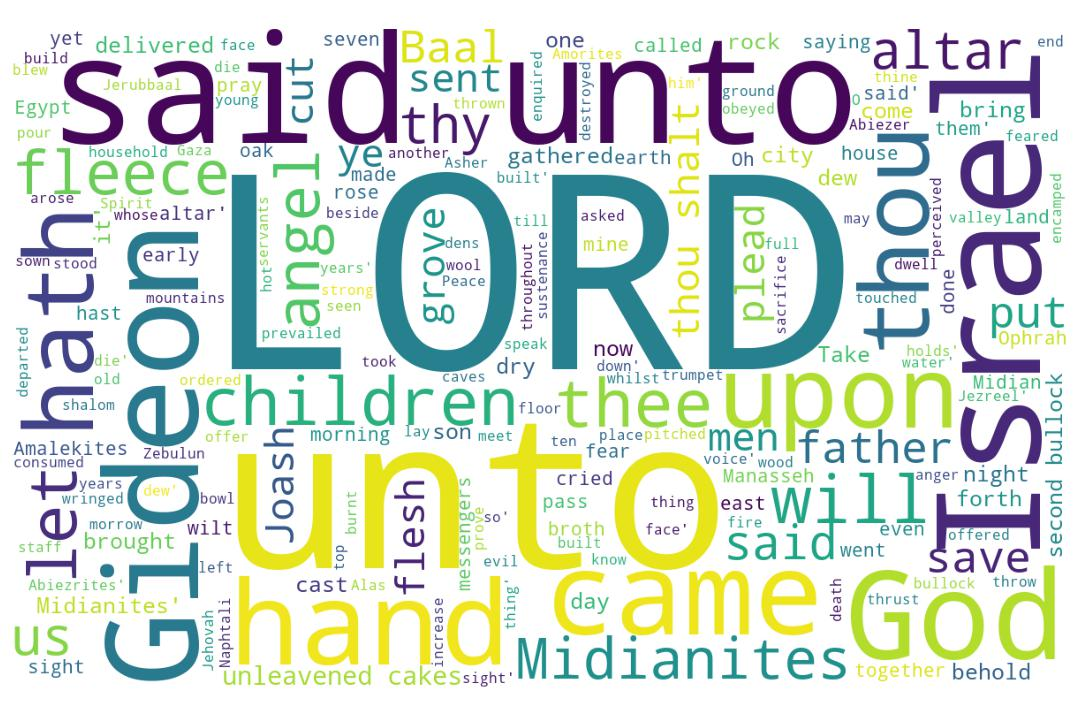
\includegraphics[width=\linewidth]{07OT-Judges/Judges6-WordCloud.jpg}
  \caption{Judges 6 Word Cloud}
  \label{fig:Judges 6 Word Cloud}
\end{figure}


\marginpar{\scriptsize \centering \fcolorbox{bone}{lime}{\textbf{GIDEON READY}}\\ (Judges 1:1-36) \begin{compactenum}[I.][8]
    \item   The  \textbf{Captivity}  \index[scripture]{Judges!Jdg 06:01} (Jdg 6:1) 
    \item   \textbf{Cave} Men \index[scripture]{Judges!Jdg 06:02} (Jdg 6:2) 
    \item   \textbf{Crops}  \index[scripture]{Judges!Jdg 06:04} (Jdg 6:4) 
    \item   The \textbf{Cry}  \index[scripture]{Judges!Jdg 06:06} (Jdg 6:6) 
    \item   Another \textbf{Champion}  \index[scripture]{Judges!Jdg 06:11} (Jdg 6:11) 
    \item   \textbf{Cakes}  \index[scripture]{Judges!Jdg 06:19--21} (Jdg 6:19--21) 
    \item   The \textbf{Conformed Ones}  \index[scripture]{Judges!Jdg 06:30} (Jdg 6:30) 
\end{compactenum}}


\footnote{\textcolor[cmyk]{0.99998,1,0,0}{\hyperlink{TOC}{Return to end of Table of Contents.}}}\footnote{\href{https://audiobible.com/bible/judges_6.html}{\textcolor[cmyk]{0.99998,1,0,0}{Judges 6 Audio}}}\textcolor[cmyk]{0.99998,1,0,0}{And the children of Israel did evil in the sight of the LORD: and the LORD delivered them into the \fcolorbox{bone}{lime}{hand of Midian} seven years.}
[2] \textcolor[cmyk]{0.99998,1,0,0}{And the hand of Midian prevailed against Israel: \emph{and} because of the Midianites the children of Israel made them the dens which \emph{are} in the mountains, and \fcolorbox{bone}{lime}{caves}, and strong holds.}
[3] \textcolor[cmyk]{0.99998,1,0,0}{And \emph{so} \fcolorbox{bone}{bone}{it} was, when Israel had sown, that the Midianites came up, and the Amalekites, and the children of the east, even they came up against them;}
[4] \textcolor[cmyk]{0.99998,1,0,0}{And they encamped against them, and destroyed the \fcolorbox{bone}{lime}{increase} of the earth, till thou come unto Gaza, and left no sustenance for Israel, neither sheep, nor ox, nor ass.}
[5] \textcolor[cmyk]{0.99998,1,0,0}{For they came up with their cattle and their tents, and they came as grasshoppers for multitude; \emph{for} both they and their camels were without number: and they entered into the land to destroy \fcolorbox{bone}{bone}{it}.}
[6] \textcolor[cmyk]{0.99998,1,0,0}{And Israel was greatly impoverished because of the Midianites; and the children of Israel \fcolorbox{bone}{lime}{cried} unto the LORD.}\\
\\
\P \textcolor[cmyk]{0.99998,1,0,0}{And \fcolorbox{bone}{bone}{it} came to pass, when the children of Israel cried unto the LORD because of the Midianites,}
[8] \textcolor[cmyk]{0.99998,1,0,0}{That the LORD sent a prophet unto the children of Israel, which said unto them, Thus saith the LORD God of Israel, I brought you up from Egypt, and brought you forth out of the house of bondage;}\
[9] \textcolor[cmyk]{0.99998,1,0,0}{And I delivered you out of the hand of the Egyptians, and out of the hand of all that oppressed you, and drave them out from before you, and gave you their land;}
[10] \textcolor[cmyk]{0.99998,1,0,0}{And I said unto you, I \emph{am} the LORD your God; fear not the gods of the Amorites, in whose land ye dwell: but ye have not obeyed my voice.}\\
\\
\P \textcolor[cmyk]{0.99998,1,0,0}{And there came an angel of the LORD, and sat under an oak which \emph{was} in Ophrah, that \emph{pertained} unto Joash the Abiezrite: and his son \fcolorbox{bone}{lime}{Gideon} threshed wheat by the winepress, to hide \emph{it} from the Midianites.}
[12] \textcolor[cmyk]{0.99998,1,0,0}{And the angel of the LORD appeared unto him, and said unto him, The LORD \emph{is} with thee, thou mighty man of valour.}
[13] \textcolor[cmyk]{0.99998,1,0,0}{And Gideon said unto him, Oh my Lord, if the LORD be with us, why then is all this befallen us? and where \emph{be} all his miracles which our fathers told us of, saying, Did not the LORD bring us up from Egypt? but now the LORD hath forsaken us, and delivered us into the hands of the Midianites.}
[14] \textcolor[cmyk]{0.99998,1,0,0}{And the LORD looked upon him, and said, Go in this thy might, and thou shalt save Israel from the hand of the Midianites: have not I sent thee?}
[15] \textcolor[cmyk]{0.99998,1,0,0}{And he said unto him, Oh my Lord, wherewith shall I save Israel? behold, my family \emph{is} poor in Manasseh, and I \emph{am} the least in my father's house.}
[16] \textcolor[cmyk]{0.99998,1,0,0}{And the LORD said unto him, Surely I will be with thee, and thou shalt smite the Midianites as one man.}
[17] \textcolor[cmyk]{0.99998,1,0,0}{And he said unto him, If now I have found grace in thy sight, then shew me a sign that thou talkest with me.}
[18] \textcolor[cmyk]{0.99998,1,0,0}{Depart not hence, I pray thee, until I come unto thee, and bring forth my present, and set \emph{it} before thee. And he said, I will tarry until thou come again.}\\
\\
\P \textcolor[cmyk]{0.99998,1,0,0}{And Gideon went in, and made ready a kid, and unleavened \fcolorbox{bone}{lime}{cakes} of an ephah of flour: the flesh he put in a basket, and he put the broth in a pot, and brought \emph{it} out unto him under the oak, and presented \emph{it}.}
[20] \textcolor[cmyk]{0.99998,1,0,0}{And the angel of God said unto him, Take the flesh and the unleavened cakes, and lay \emph{them} upon this rock, and pour out the broth. And he did so.}\\
\\
\P \textcolor[cmyk]{0.99998,1,0,0}{Then the angel of the LORD put forth the end of the staff that \emph{was} in his hand, and touched the flesh and the unleavened cakes; and there rose up fire out of the rock, and consumed the flesh and the unleavened cakes. Then the angel of the LORD departed out of his sight.}
[22] \textcolor[cmyk]{0.99998,1,0,0}{And when Gideon perceived that he \emph{was} an angel of the LORD, Gideon said, Alas, O Lord GOD! for because I have seen an angel of the LORD face to face.}
[23] \textcolor[cmyk]{0.99998,1,0,0}{And the LORD said unto him, Peace \emph{be} unto thee; fear not: thou shalt not die.}
[24] \textcolor[cmyk]{0.99998,1,0,0}{Then Gideon built an altar there unto the LORD, and called \fcolorbox{bone}{bone}{it} Jehovah-shalom: unto this day \fcolorbox{bone}{bone}{it} \emph{is} yet in Ophrah of the Abiezrites.}\\
\\
\P \textcolor[cmyk]{0.99998,1,0,0}{And \fcolorbox{bone}{bone}{it} came to pass the same night, that the LORD said unto him, Take thy father's young bullock, even the second bullock of seven years old, and throw down the altar of Baal that thy father hath, and cut down the grove that \emph{is} by \fcolorbox{bone}{bone}{it}:}
[26] \textcolor[cmyk]{0.99998,1,0,0}{And build an altar unto the LORD thy God upon the top of this rock, in the ordered place, and take the second bullock, and offer a burnt sacrifice with the wood of the grove which thou shalt cut down.}
[27] \textcolor[cmyk]{0.99998,1,0,0}{Then Gideon took ten men of his servants, and did as the LORD had said unto him: and \emph{so} \fcolorbox{bone}{bone}{it} was, because he feared his father's household, and the men of the city, that he could not do \emph{it} by day, that he did \emph{it} by night.}\\
\\
\P \textcolor[cmyk]{0.99998,1,0,0}{And when the men of the city arose early in the morning, behold, the altar of Baal was cast down, and the grove was cut down that \emph{was} by \fcolorbox{bone}{bone}{it}, and the second bullock was offered upon the altar \emph{that} \emph{was} built.}
[29] \textcolor[cmyk]{0.99998,1,0,0}{And they said one to another, Who hath done this thing? And when they enquired and asked, they said, Gideon the son of Joash hath done this thing.}
[30] \textcolor[cmyk]{0.99998,1,0,0}{Then the \fcolorbox{bone}{lime}{men of the city} said unto Joash, Bring out thy son, that he may die: because he hath cast down the altar of Baal, and because he hath cut down the grove that \emph{was} by \fcolorbox{bone}{bone}{it}.}
[31] \textcolor[cmyk]{0.99998,1,0,0}{And Joash said unto all that stood against him, Will ye plead for Baal? will ye save him? he that will plead for him, let him be put to death whilst \emph{it} \emph{is} \emph{yet} morning: if he \emph{be} a god, let him plead for himself, because \emph{one} hath cast down his altar.}
[32] \textcolor[cmyk]{0.99998,1,0,0}{Therefore on that day he called him Jerubbaal, saying, Let Baal plead against him, because he hath thrown down his altar.}\\
\\
\P \textcolor[cmyk]{0.99998,1,0,0}{Then all the Midianites and the Amalekites and the children of the east were gathered together, and went over, and pitched in the valley of Jezreel.}
[34] \textcolor[cmyk]{0.99998,1,0,0}{But the Spirit of the LORD came upon Gideon, and he blew a trumpet; and Abiezer was gathered after him.}
[35] \textcolor[cmyk]{0.99998,1,0,0}{And he sent messengers throughout all Manasseh; who also was gathered after him: and he sent messengers unto Asher, and unto Zebulun, and unto Naphtali; and they came up to meet them.}\\
\\
\P \textcolor[cmyk]{0.99998,1,0,0}{And Gideon said unto God, If thou wilt save Israel by mine hand, as thou hast said,}
[37] \textcolor[cmyk]{0.99998,1,0,0}{Behold, I will put a fleece of wool in the floor; \emph{and} if the dew be on the fleece only, and \emph{it} \emph{be} dry upon all the earth \emph{beside}, then shall I know that thou wilt save Israel by mine hand, as thou hast said.}
[38] \textcolor[cmyk]{0.99998,1,0,0}{And \fcolorbox{bone}{bone}{it} was so: for he rose up early on the morrow, and thrust the fleece together, and wringed the dew out of the fleece, a bowl full of water.}
[39] \textcolor[cmyk]{0.99998,1,0,0}{And Gideon said unto God, Let not thine anger be hot against me, and I will speak but this once: let me prove, I pray thee, but this once with the fleece; let \fcolorbox{bone}{bone}{it} now be dry only upon the fleece, and upon all the ground let there be dew.}
[40] \textcolor[cmyk]{0.99998,1,0,0}{And God did so that night: for \fcolorbox{bone}{bone}{it} was dry upon the fleece only, and there was dew on all the ground.}
\index[NWIV]{25!Judges!Jud 6:1}\index[AWIP]{And!Judges!Jud 6:1}\index[AWIP]{the!Judges!Jud 6:1}\index[AWIP]{the!Judges!Jud 6:1 (2)}\index[AWIP]{the!Judges!Jud 6:1 (3)}\index[AWIP]{the!Judges!Jud 6:1 (4)}\index[AWIP]{the!Judges!Jud 6:1 (5)}\index[AWIP]{children!Judges!Jud 6:1}\index[AWIP]{of!Judges!Jud 6:1}\index[AWIP]{of!Judges!Jud 6:1 (2)}\index[AWIP]{of!Judges!Jud 6:1 (3)}\index[AWIP]{Israel!Judges!Jud 6:1}\index[AWIP]{did!Judges!Jud 6:1}\index[AWIP]{evil!Judges!Jud 6:1}\index[AWIP]{in!Judges!Jud 6:1}\index[AWIP]{sight!Judges!Jud 6:1}\index[AWIP]{LORD!Judges!Jud 6:1}\index[AWIP]{LORD!Judges!Jud 6:1 (2)}\index[AWIP]{and!Judges!Jud 6:1}\index[AWIP]{delivered!Judges!Jud 6:1}\index[AWIP]{them!Judges!Jud 6:1}\index[AWIP]{into!Judges!Jud 6:1}\index[AWIP]{hand!Judges!Jud 6:1}\index[AWIP]{Midian!Judges!Jud 6:1}\index[AWIP]{seven!Judges!Jud 6:1}\index[AWIP]{years!Judges!Jud 6:1}

\index[NWIV]{31!Judges!Jud 6:2}\index[AWIP]{And!Judges!Jud 6:2}\index[AWIP]{the!Judges!Jud 6:2}\index[AWIP]{the!Judges!Jud 6:2 (2)}\index[AWIP]{the!Judges!Jud 6:2 (3)}\index[AWIP]{the!Judges!Jud 6:2 (4)}\index[AWIP]{the!Judges!Jud 6:2 (5)}\index[AWIP]{hand!Judges!Jud 6:2}\index[AWIP]{of!Judges!Jud 6:2}\index[AWIP]{of!Judges!Jud 6:2 (2)}\index[AWIP]{of!Judges!Jud 6:2 (3)}\index[AWIP]{Midian!Judges!Jud 6:2}\index[AWIP]{prevailed!Judges!Jud 6:2}\index[AWIP]{against!Judges!Jud 6:2}\index[AWIP]{Israel!Judges!Jud 6:2}\index[AWIP]{Israel!Judges!Jud 6:2 (2)}\index[AWIP]{\emph{and}!Judges!Jud 6:2}\index[AWIP]{because!Judges!Jud 6:2}\index[AWIP]{Midianites!Judges!Jud 6:2}\index[AWIP]{children!Judges!Jud 6:2}\index[AWIP]{made!Judges!Jud 6:2}\index[AWIP]{them!Judges!Jud 6:2}\index[AWIP]{dens!Judges!Jud 6:2}\index[AWIP]{which!Judges!Jud 6:2}\index[AWIP]{\emph{are}!Judges!Jud 6:2}\index[AWIP]{in!Judges!Jud 6:2}\index[AWIP]{mountains!Judges!Jud 6:2}\index[AWIP]{and!Judges!Jud 6:2}\index[AWIP]{and!Judges!Jud 6:2 (2)}\index[AWIP]{caves!Judges!Jud 6:2}\index[AWIP]{strong!Judges!Jud 6:2}\index[AWIP]{holds!Judges!Jud 6:2}\index[AWIP]{\emph{and}!Judges!Jud 6:2}\index[AWIP]{\emph{are}!Judges!Jud 6:2}

\index[NWIV]{28!Judges!Jud 6:3}\index[AWIP]{And!Judges!Jud 6:3}\index[AWIP]{\emph{so}!Judges!Jud 6:3}\index[AWIP]{it!Judges!Jud 6:3}\index[AWIP]{was!Judges!Jud 6:3}\index[AWIP]{when!Judges!Jud 6:3}\index[AWIP]{Israel!Judges!Jud 6:3}\index[AWIP]{had!Judges!Jud 6:3}\index[AWIP]{sown!Judges!Jud 6:3}\index[AWIP]{that!Judges!Jud 6:3}\index[AWIP]{the!Judges!Jud 6:3}\index[AWIP]{the!Judges!Jud 6:3 (2)}\index[AWIP]{the!Judges!Jud 6:3 (3)}\index[AWIP]{the!Judges!Jud 6:3 (4)}\index[AWIP]{Midianites!Judges!Jud 6:3}\index[AWIP]{came!Judges!Jud 6:3}\index[AWIP]{came!Judges!Jud 6:3 (2)}\index[AWIP]{up!Judges!Jud 6:3}\index[AWIP]{up!Judges!Jud 6:3 (2)}\index[AWIP]{and!Judges!Jud 6:3}\index[AWIP]{and!Judges!Jud 6:3 (2)}\index[AWIP]{Amalekites!Judges!Jud 6:3}\index[AWIP]{children!Judges!Jud 6:3}\index[AWIP]{of!Judges!Jud 6:3}\index[AWIP]{east!Judges!Jud 6:3}\index[AWIP]{even!Judges!Jud 6:3}\index[AWIP]{they!Judges!Jud 6:3}\index[AWIP]{against!Judges!Jud 6:3}\index[AWIP]{them!Judges!Jud 6:3}\index[AWIP]{\emph{so}!Judges!Jud 6:3}

\index[NWIV]{29!Judges!Jud 6:4}\index[AWIP]{And!Judges!Jud 6:4}\index[AWIP]{they!Judges!Jud 6:4}\index[AWIP]{encamped!Judges!Jud 6:4}\index[AWIP]{against!Judges!Jud 6:4}\index[AWIP]{them!Judges!Jud 6:4}\index[AWIP]{and!Judges!Jud 6:4}\index[AWIP]{and!Judges!Jud 6:4 (2)}\index[AWIP]{destroyed!Judges!Jud 6:4}\index[AWIP]{the!Judges!Jud 6:4}\index[AWIP]{the!Judges!Jud 6:4 (2)}\index[AWIP]{increase!Judges!Jud 6:4}\index[AWIP]{of!Judges!Jud 6:4}\index[AWIP]{earth!Judges!Jud 6:4}\index[AWIP]{till!Judges!Jud 6:4}\index[AWIP]{thou!Judges!Jud 6:4}\index[AWIP]{come!Judges!Jud 6:4}\index[AWIP]{unto!Judges!Jud 6:4}\index[AWIP]{Gaza!Judges!Jud 6:4}\index[AWIP]{left!Judges!Jud 6:4}\index[AWIP]{no!Judges!Jud 6:4}\index[AWIP]{sustenance!Judges!Jud 6:4}\index[AWIP]{for!Judges!Jud 6:4}\index[AWIP]{Israel!Judges!Jud 6:4}\index[AWIP]{neither!Judges!Jud 6:4}\index[AWIP]{sheep!Judges!Jud 6:4}\index[AWIP]{nor!Judges!Jud 6:4}\index[AWIP]{nor!Judges!Jud 6:4 (2)}\index[AWIP]{ox!Judges!Jud 6:4}\index[AWIP]{ass!Judges!Jud 6:4}

\index[NWIV]{35!Judges!Jud 6:5}\index[AWIP]{For!Judges!Jud 6:5}\index[AWIP]{they!Judges!Jud 6:5}\index[AWIP]{they!Judges!Jud 6:5 (2)}\index[AWIP]{they!Judges!Jud 6:5 (3)}\index[AWIP]{they!Judges!Jud 6:5 (4)}\index[AWIP]{came!Judges!Jud 6:5}\index[AWIP]{came!Judges!Jud 6:5 (2)}\index[AWIP]{up!Judges!Jud 6:5}\index[AWIP]{with!Judges!Jud 6:5}\index[AWIP]{their!Judges!Jud 6:5}\index[AWIP]{their!Judges!Jud 6:5 (2)}\index[AWIP]{their!Judges!Jud 6:5 (3)}\index[AWIP]{cattle!Judges!Jud 6:5}\index[AWIP]{and!Judges!Jud 6:5}\index[AWIP]{and!Judges!Jud 6:5 (2)}\index[AWIP]{and!Judges!Jud 6:5 (3)}\index[AWIP]{and!Judges!Jud 6:5 (4)}\index[AWIP]{tents!Judges!Jud 6:5}\index[AWIP]{as!Judges!Jud 6:5}\index[AWIP]{grasshoppers!Judges!Jud 6:5}\index[AWIP]{for!Judges!Jud 6:5}\index[AWIP]{multitude!Judges!Jud 6:5}\index[AWIP]{\emph{for}!Judges!Jud 6:5}\index[AWIP]{both!Judges!Jud 6:5}\index[AWIP]{camels!Judges!Jud 6:5}\index[AWIP]{were!Judges!Jud 6:5}\index[AWIP]{without!Judges!Jud 6:5}\index[AWIP]{number!Judges!Jud 6:5}\index[AWIP]{entered!Judges!Jud 6:5}\index[AWIP]{into!Judges!Jud 6:5}\index[AWIP]{the!Judges!Jud 6:5}\index[AWIP]{land!Judges!Jud 6:5}\index[AWIP]{to!Judges!Jud 6:5}\index[AWIP]{destroy!Judges!Jud 6:5}\index[AWIP]{it!Judges!Jud 6:5}\index[AWIP]{\emph{for}!Judges!Jud 6:5}

\index[NWIV]{18!Judges!Jud 6:6}\index[AWIP]{And!Judges!Jud 6:6}\index[AWIP]{Israel!Judges!Jud 6:6}\index[AWIP]{Israel!Judges!Jud 6:6 (2)}\index[AWIP]{was!Judges!Jud 6:6}\index[AWIP]{greatly!Judges!Jud 6:6}\index[AWIP]{impoverished!Judges!Jud 6:6}\index[AWIP]{because!Judges!Jud 6:6}\index[AWIP]{of!Judges!Jud 6:6}\index[AWIP]{of!Judges!Jud 6:6 (2)}\index[AWIP]{the!Judges!Jud 6:6}\index[AWIP]{the!Judges!Jud 6:6 (2)}\index[AWIP]{the!Judges!Jud 6:6 (3)}\index[AWIP]{Midianites!Judges!Jud 6:6}\index[AWIP]{and!Judges!Jud 6:6}\index[AWIP]{children!Judges!Jud 6:6}\index[AWIP]{cried!Judges!Jud 6:6}\index[AWIP]{unto!Judges!Jud 6:6}\index[AWIP]{LORD!Judges!Jud 6:6}

\index[NWIV]{18!Judges!Jud 6:7}\index[AWIP]{And!Judges!Jud 6:7}\index[AWIP]{it!Judges!Jud 6:7}\index[AWIP]{came!Judges!Jud 6:7}\index[AWIP]{to!Judges!Jud 6:7}\index[AWIP]{pass!Judges!Jud 6:7}\index[AWIP]{when!Judges!Jud 6:7}\index[AWIP]{the!Judges!Jud 6:7}\index[AWIP]{the!Judges!Jud 6:7 (2)}\index[AWIP]{the!Judges!Jud 6:7 (3)}\index[AWIP]{children!Judges!Jud 6:7}\index[AWIP]{of!Judges!Jud 6:7}\index[AWIP]{of!Judges!Jud 6:7 (2)}\index[AWIP]{Israel!Judges!Jud 6:7}\index[AWIP]{cried!Judges!Jud 6:7}\index[AWIP]{unto!Judges!Jud 6:7}\index[AWIP]{LORD!Judges!Jud 6:7}\index[AWIP]{because!Judges!Jud 6:7}\index[AWIP]{Midianites!Judges!Jud 6:7}

\index[NWIV]{38!Judges!Jud 6:8}\index[AWIP]{That!Judges!Jud 6:8}\index[AWIP]{the!Judges!Jud 6:8}\index[AWIP]{the!Judges!Jud 6:8 (2)}\index[AWIP]{the!Judges!Jud 6:8 (3)}\index[AWIP]{the!Judges!Jud 6:8 (4)}\index[AWIP]{LORD!Judges!Jud 6:8}\index[AWIP]{LORD!Judges!Jud 6:8 (2)}\index[AWIP]{sent!Judges!Jud 6:8}\index[AWIP]{a!Judges!Jud 6:8}\index[AWIP]{prophet!Judges!Jud 6:8}\index[AWIP]{unto!Judges!Jud 6:8}\index[AWIP]{unto!Judges!Jud 6:8 (2)}\index[AWIP]{children!Judges!Jud 6:8}\index[AWIP]{of!Judges!Jud 6:8}\index[AWIP]{of!Judges!Jud 6:8 (2)}\index[AWIP]{of!Judges!Jud 6:8 (3)}\index[AWIP]{of!Judges!Jud 6:8 (4)}\index[AWIP]{Israel!Judges!Jud 6:8}\index[AWIP]{Israel!Judges!Jud 6:8 (2)}\index[AWIP]{which!Judges!Jud 6:8}\index[AWIP]{said!Judges!Jud 6:8}\index[AWIP]{them!Judges!Jud 6:8}\index[AWIP]{Thus!Judges!Jud 6:8}\index[AWIP]{saith!Judges!Jud 6:8}\index[AWIP]{God!Judges!Jud 6:8}\index[AWIP]{I!Judges!Jud 6:8}\index[AWIP]{brought!Judges!Jud 6:8}\index[AWIP]{brought!Judges!Jud 6:8 (2)}\index[AWIP]{you!Judges!Jud 6:8}\index[AWIP]{you!Judges!Jud 6:8 (2)}\index[AWIP]{up!Judges!Jud 6:8}\index[AWIP]{from!Judges!Jud 6:8}\index[AWIP]{Egypt!Judges!Jud 6:8}\index[AWIP]{and!Judges!Jud 6:8}\index[AWIP]{forth!Judges!Jud 6:8}\index[AWIP]{out!Judges!Jud 6:8}\index[AWIP]{house!Judges!Jud 6:8}\index[AWIP]{bondage!Judges!Jud 6:8}

\index[NWIV]{33!Judges!Jud 6:9}\index[AWIP]{And!Judges!Jud 6:9}\index[AWIP]{I!Judges!Jud 6:9}\index[AWIP]{delivered!Judges!Jud 6:9}\index[AWIP]{you!Judges!Jud 6:9}\index[AWIP]{you!Judges!Jud 6:9 (2)}\index[AWIP]{you!Judges!Jud 6:9 (3)}\index[AWIP]{you!Judges!Jud 6:9 (4)}\index[AWIP]{out!Judges!Jud 6:9}\index[AWIP]{out!Judges!Jud 6:9 (2)}\index[AWIP]{out!Judges!Jud 6:9 (3)}\index[AWIP]{of!Judges!Jud 6:9}\index[AWIP]{of!Judges!Jud 6:9 (2)}\index[AWIP]{of!Judges!Jud 6:9 (3)}\index[AWIP]{of!Judges!Jud 6:9 (4)}\index[AWIP]{the!Judges!Jud 6:9}\index[AWIP]{the!Judges!Jud 6:9 (2)}\index[AWIP]{the!Judges!Jud 6:9 (3)}\index[AWIP]{hand!Judges!Jud 6:9}\index[AWIP]{hand!Judges!Jud 6:9 (2)}\index[AWIP]{Egyptians!Judges!Jud 6:9}\index[AWIP]{and!Judges!Jud 6:9}\index[AWIP]{and!Judges!Jud 6:9 (2)}\index[AWIP]{and!Judges!Jud 6:9 (3)}\index[AWIP]{all!Judges!Jud 6:9}\index[AWIP]{that!Judges!Jud 6:9}\index[AWIP]{oppressed!Judges!Jud 6:9}\index[AWIP]{drave!Judges!Jud 6:9}\index[AWIP]{them!Judges!Jud 6:9}\index[AWIP]{from!Judges!Jud 6:9}\index[AWIP]{before!Judges!Jud 6:9}\index[AWIP]{gave!Judges!Jud 6:9}\index[AWIP]{their!Judges!Jud 6:9}\index[AWIP]{land!Judges!Jud 6:9}

\index[NWIV]{30!Judges!Jud 6:10}\index[AWIP]{And!Judges!Jud 6:10}\index[AWIP]{I!Judges!Jud 6:10}\index[AWIP]{I!Judges!Jud 6:10 (2)}\index[AWIP]{said!Judges!Jud 6:10}\index[AWIP]{unto!Judges!Jud 6:10}\index[AWIP]{you!Judges!Jud 6:10}\index[AWIP]{\emph{am}!Judges!Jud 6:10}\index[AWIP]{the!Judges!Jud 6:10}\index[AWIP]{the!Judges!Jud 6:10 (2)}\index[AWIP]{the!Judges!Jud 6:10 (3)}\index[AWIP]{LORD!Judges!Jud 6:10}\index[AWIP]{your!Judges!Jud 6:10}\index[AWIP]{God!Judges!Jud 6:10}\index[AWIP]{fear!Judges!Jud 6:10}\index[AWIP]{not!Judges!Jud 6:10}\index[AWIP]{not!Judges!Jud 6:10 (2)}\index[AWIP]{gods!Judges!Jud 6:10}\index[AWIP]{of!Judges!Jud 6:10}\index[AWIP]{Amorites!Judges!Jud 6:10}\index[AWIP]{in!Judges!Jud 6:10}\index[AWIP]{whose!Judges!Jud 6:10}\index[AWIP]{land!Judges!Jud 6:10}\index[AWIP]{ye!Judges!Jud 6:10}\index[AWIP]{ye!Judges!Jud 6:10 (2)}\index[AWIP]{dwell!Judges!Jud 6:10}\index[AWIP]{but!Judges!Jud 6:10}\index[AWIP]{have!Judges!Jud 6:10}\index[AWIP]{obeyed!Judges!Jud 6:10}\index[AWIP]{my!Judges!Jud 6:10}\index[AWIP]{voice!Judges!Jud 6:10}\index[AWIP]{\emph{am}!Judges!Jud 6:10}

\index[NWIV]{38!Judges!Jud 6:11}\index[AWIP]{And!Judges!Jud 6:11}\index[AWIP]{there!Judges!Jud 6:11}\index[AWIP]{came!Judges!Jud 6:11}\index[AWIP]{an!Judges!Jud 6:11}\index[AWIP]{an!Judges!Jud 6:11 (2)}\index[AWIP]{angel!Judges!Jud 6:11}\index[AWIP]{of!Judges!Jud 6:11}\index[AWIP]{the!Judges!Jud 6:11}\index[AWIP]{the!Judges!Jud 6:11 (2)}\index[AWIP]{the!Judges!Jud 6:11 (3)}\index[AWIP]{the!Judges!Jud 6:11 (4)}\index[AWIP]{LORD!Judges!Jud 6:11}\index[AWIP]{and!Judges!Jud 6:11}\index[AWIP]{and!Judges!Jud 6:11 (2)}\index[AWIP]{sat!Judges!Jud 6:11}\index[AWIP]{under!Judges!Jud 6:11}\index[AWIP]{oak!Judges!Jud 6:11}\index[AWIP]{which!Judges!Jud 6:11}\index[AWIP]{\emph{was}!Judges!Jud 6:11}\index[AWIP]{in!Judges!Jud 6:11}\index[AWIP]{Ophrah!Judges!Jud 6:11}\index[AWIP]{that!Judges!Jud 6:11}\index[AWIP]{\emph{pertained}!Judges!Jud 6:11}\index[AWIP]{unto!Judges!Jud 6:11}\index[AWIP]{Joash!Judges!Jud 6:11}\index[AWIP]{Abiezrite!Judges!Jud 6:11}\index[AWIP]{his!Judges!Jud 6:11}\index[AWIP]{son!Judges!Jud 6:11}\index[AWIP]{Gideon!Judges!Jud 6:11}\index[AWIP]{threshed!Judges!Jud 6:11}\index[AWIP]{wheat!Judges!Jud 6:11}\index[AWIP]{by!Judges!Jud 6:11}\index[AWIP]{winepress!Judges!Jud 6:11}\index[AWIP]{to!Judges!Jud 6:11}\index[AWIP]{hide!Judges!Jud 6:11}\index[AWIP]{\emph{it}!Judges!Jud 6:11}\index[AWIP]{from!Judges!Jud 6:11}\index[AWIP]{Midianites!Judges!Jud 6:11}\index[AWIP]{\emph{was}!Judges!Jud 6:11}\index[AWIP]{\emph{pertained}!Judges!Jud 6:11}\index[AWIP]{\emph{it}!Judges!Jud 6:11}

\index[NWIV]{23!Judges!Jud 6:12}\index[AWIP]{And!Judges!Jud 6:12}\index[AWIP]{the!Judges!Jud 6:12}\index[AWIP]{the!Judges!Jud 6:12 (2)}\index[AWIP]{angel!Judges!Jud 6:12}\index[AWIP]{of!Judges!Jud 6:12}\index[AWIP]{of!Judges!Jud 6:12 (2)}\index[AWIP]{LORD!Judges!Jud 6:12}\index[AWIP]{LORD!Judges!Jud 6:12 (2)}\index[AWIP]{appeared!Judges!Jud 6:12}\index[AWIP]{unto!Judges!Jud 6:12}\index[AWIP]{unto!Judges!Jud 6:12 (2)}\index[AWIP]{him!Judges!Jud 6:12}\index[AWIP]{him!Judges!Jud 6:12 (2)}\index[AWIP]{and!Judges!Jud 6:12}\index[AWIP]{said!Judges!Jud 6:12}\index[AWIP]{The!Judges!Jud 6:12}\index[AWIP]{\emph{is}!Judges!Jud 6:12}\index[AWIP]{with!Judges!Jud 6:12}\index[AWIP]{thee!Judges!Jud 6:12}\index[AWIP]{thou!Judges!Jud 6:12}\index[AWIP]{mighty!Judges!Jud 6:12}\index[AWIP]{man!Judges!Jud 6:12}\index[AWIP]{valour!Judges!Jud 6:12}\index[AWIP]{\emph{is}!Judges!Jud 6:12}

\index[NWIV]{59!Judges!Jud 6:13}\index[AWIP]{And!Judges!Jud 6:13}\index[AWIP]{Gideon!Judges!Jud 6:13}\index[AWIP]{said!Judges!Jud 6:13}\index[AWIP]{unto!Judges!Jud 6:13}\index[AWIP]{him!Judges!Jud 6:13}\index[AWIP]{Oh!Judges!Jud 6:13}\index[AWIP]{my!Judges!Jud 6:13}\index[AWIP]{Lord!Judges!Jud 6:13}\index[AWIP]{if!Judges!Jud 6:13}\index[AWIP]{the!Judges!Jud 6:13}\index[AWIP]{the!Judges!Jud 6:13 (2)}\index[AWIP]{the!Judges!Jud 6:13 (3)}\index[AWIP]{the!Judges!Jud 6:13 (4)}\index[AWIP]{the!Judges!Jud 6:13 (5)}\index[AWIP]{LORD!Judges!Jud 6:13}\index[AWIP]{LORD!Judges!Jud 6:13 (2)}\index[AWIP]{LORD!Judges!Jud 6:13 (3)}\index[AWIP]{be!Judges!Jud 6:13}\index[AWIP]{with!Judges!Jud 6:13}\index[AWIP]{us!Judges!Jud 6:13}\index[AWIP]{us!Judges!Jud 6:13 (2)}\index[AWIP]{us!Judges!Jud 6:13 (3)}\index[AWIP]{us!Judges!Jud 6:13 (4)}\index[AWIP]{us!Judges!Jud 6:13 (5)}\index[AWIP]{why!Judges!Jud 6:13}\index[AWIP]{then!Judges!Jud 6:13}\index[AWIP]{is!Judges!Jud 6:13}\index[AWIP]{all!Judges!Jud 6:13}\index[AWIP]{all!Judges!Jud 6:13 (2)}\index[AWIP]{this!Judges!Jud 6:13}\index[AWIP]{befallen!Judges!Jud 6:13}\index[AWIP]{us?!Judges!Jud 6:13}\index[AWIP]{and!Judges!Jud 6:13}\index[AWIP]{and!Judges!Jud 6:13 (2)}\index[AWIP]{where!Judges!Jud 6:13}\index[AWIP]{\emph{be}!Judges!Jud 6:13}\index[AWIP]{his!Judges!Jud 6:13}\index[AWIP]{miracles!Judges!Jud 6:13}\index[AWIP]{which!Judges!Jud 6:13}\index[AWIP]{our!Judges!Jud 6:13}\index[AWIP]{fathers!Judges!Jud 6:13}\index[AWIP]{told!Judges!Jud 6:13}\index[AWIP]{of!Judges!Jud 6:13}\index[AWIP]{of!Judges!Jud 6:13 (2)}\index[AWIP]{saying!Judges!Jud 6:13}\index[AWIP]{Did!Judges!Jud 6:13}\index[AWIP]{not!Judges!Jud 6:13}\index[AWIP]{bring!Judges!Jud 6:13}\index[AWIP]{up!Judges!Jud 6:13}\index[AWIP]{from!Judges!Jud 6:13}\index[AWIP]{Egypt?!Judges!Jud 6:13}\index[AWIP]{but!Judges!Jud 6:13}\index[AWIP]{now!Judges!Jud 6:13}\index[AWIP]{hath!Judges!Jud 6:13}\index[AWIP]{forsaken!Judges!Jud 6:13}\index[AWIP]{delivered!Judges!Jud 6:13}\index[AWIP]{into!Judges!Jud 6:13}\index[AWIP]{hands!Judges!Jud 6:13}\index[AWIP]{Midianites!Judges!Jud 6:13}\index[AWIP]{\emph{be}!Judges!Jud 6:13}

\index[NWIV]{29!Judges!Jud 6:14}\index[AWIP]{And!Judges!Jud 6:14}\index[AWIP]{the!Judges!Jud 6:14}\index[AWIP]{the!Judges!Jud 6:14 (2)}\index[AWIP]{the!Judges!Jud 6:14 (3)}\index[AWIP]{LORD!Judges!Jud 6:14}\index[AWIP]{looked!Judges!Jud 6:14}\index[AWIP]{upon!Judges!Jud 6:14}\index[AWIP]{him!Judges!Jud 6:14}\index[AWIP]{and!Judges!Jud 6:14}\index[AWIP]{and!Judges!Jud 6:14 (2)}\index[AWIP]{said!Judges!Jud 6:14}\index[AWIP]{Go!Judges!Jud 6:14}\index[AWIP]{in!Judges!Jud 6:14}\index[AWIP]{this!Judges!Jud 6:14}\index[AWIP]{thy!Judges!Jud 6:14}\index[AWIP]{might!Judges!Jud 6:14}\index[AWIP]{thou!Judges!Jud 6:14}\index[AWIP]{shalt!Judges!Jud 6:14}\index[AWIP]{save!Judges!Jud 6:14}\index[AWIP]{Israel!Judges!Jud 6:14}\index[AWIP]{from!Judges!Jud 6:14}\index[AWIP]{hand!Judges!Jud 6:14}\index[AWIP]{of!Judges!Jud 6:14}\index[AWIP]{Midianites!Judges!Jud 6:14}\index[AWIP]{have!Judges!Jud 6:14}\index[AWIP]{not!Judges!Jud 6:14}\index[AWIP]{I!Judges!Jud 6:14}\index[AWIP]{sent!Judges!Jud 6:14}\index[AWIP]{thee?!Judges!Jud 6:14}

\index[NWIV]{29!Judges!Jud 6:15}\index[AWIP]{And!Judges!Jud 6:15}\index[AWIP]{he!Judges!Jud 6:15}\index[AWIP]{said!Judges!Jud 6:15}\index[AWIP]{unto!Judges!Jud 6:15}\index[AWIP]{him!Judges!Jud 6:15}\index[AWIP]{Oh!Judges!Jud 6:15}\index[AWIP]{my!Judges!Jud 6:15}\index[AWIP]{my!Judges!Jud 6:15 (2)}\index[AWIP]{my!Judges!Jud 6:15 (3)}\index[AWIP]{Lord!Judges!Jud 6:15}\index[AWIP]{wherewith!Judges!Jud 6:15}\index[AWIP]{shall!Judges!Jud 6:15}\index[AWIP]{I!Judges!Jud 6:15}\index[AWIP]{I!Judges!Jud 6:15 (2)}\index[AWIP]{save!Judges!Jud 6:15}\index[AWIP]{Israel?!Judges!Jud 6:15}\index[AWIP]{behold!Judges!Jud 6:15}\index[AWIP]{family!Judges!Jud 6:15}\index[AWIP]{\emph{is}!Judges!Jud 6:15}\index[AWIP]{poor!Judges!Jud 6:15}\index[AWIP]{in!Judges!Jud 6:15}\index[AWIP]{in!Judges!Jud 6:15 (2)}\index[AWIP]{Manasseh!Judges!Jud 6:15}\index[AWIP]{and!Judges!Jud 6:15}\index[AWIP]{\emph{am}!Judges!Jud 6:15}\index[AWIP]{the!Judges!Jud 6:15}\index[AWIP]{least!Judges!Jud 6:15}\index[AWIP]{father's!Judges!Jud 6:15}\index[AWIP]{house!Judges!Jud 6:15}\index[AWIP]{\emph{is}!Judges!Jud 6:15}\index[AWIP]{\emph{am}!Judges!Jud 6:15}

\index[NWIV]{21!Judges!Jud 6:16}\index[AWIP]{And!Judges!Jud 6:16}\index[AWIP]{the!Judges!Jud 6:16}\index[AWIP]{the!Judges!Jud 6:16 (2)}\index[AWIP]{LORD!Judges!Jud 6:16}\index[AWIP]{said!Judges!Jud 6:16}\index[AWIP]{unto!Judges!Jud 6:16}\index[AWIP]{him!Judges!Jud 6:16}\index[AWIP]{Surely!Judges!Jud 6:16}\index[AWIP]{I!Judges!Jud 6:16}\index[AWIP]{will!Judges!Jud 6:16}\index[AWIP]{be!Judges!Jud 6:16}\index[AWIP]{with!Judges!Jud 6:16}\index[AWIP]{thee!Judges!Jud 6:16}\index[AWIP]{and!Judges!Jud 6:16}\index[AWIP]{thou!Judges!Jud 6:16}\index[AWIP]{shalt!Judges!Jud 6:16}\index[AWIP]{smite!Judges!Jud 6:16}\index[AWIP]{Midianites!Judges!Jud 6:16}\index[AWIP]{as!Judges!Jud 6:16}\index[AWIP]{one!Judges!Jud 6:16}\index[AWIP]{man!Judges!Jud 6:16}

\index[NWIV]{24!Judges!Jud 6:17}\index[AWIP]{And!Judges!Jud 6:17}\index[AWIP]{he!Judges!Jud 6:17}\index[AWIP]{said!Judges!Jud 6:17}\index[AWIP]{unto!Judges!Jud 6:17}\index[AWIP]{him!Judges!Jud 6:17}\index[AWIP]{If!Judges!Jud 6:17}\index[AWIP]{now!Judges!Jud 6:17}\index[AWIP]{I!Judges!Jud 6:17}\index[AWIP]{have!Judges!Jud 6:17}\index[AWIP]{found!Judges!Jud 6:17}\index[AWIP]{grace!Judges!Jud 6:17}\index[AWIP]{in!Judges!Jud 6:17}\index[AWIP]{thy!Judges!Jud 6:17}\index[AWIP]{sight!Judges!Jud 6:17}\index[AWIP]{then!Judges!Jud 6:17}\index[AWIP]{shew!Judges!Jud 6:17}\index[AWIP]{me!Judges!Jud 6:17}\index[AWIP]{me!Judges!Jud 6:17 (2)}\index[AWIP]{a!Judges!Jud 6:17}\index[AWIP]{sign!Judges!Jud 6:17}\index[AWIP]{that!Judges!Jud 6:17}\index[AWIP]{thou!Judges!Jud 6:17}\index[AWIP]{talkest!Judges!Jud 6:17}\index[AWIP]{with!Judges!Jud 6:17}

\index[NWIV]{31!Judges!Jud 6:18}\index[AWIP]{Depart!Judges!Jud 6:18}\index[AWIP]{not!Judges!Jud 6:18}\index[AWIP]{hence!Judges!Jud 6:18}\index[AWIP]{I!Judges!Jud 6:18}\index[AWIP]{I!Judges!Jud 6:18 (2)}\index[AWIP]{I!Judges!Jud 6:18 (3)}\index[AWIP]{pray!Judges!Jud 6:18}\index[AWIP]{thee!Judges!Jud 6:18}\index[AWIP]{thee!Judges!Jud 6:18 (2)}\index[AWIP]{thee!Judges!Jud 6:18 (3)}\index[AWIP]{until!Judges!Jud 6:18}\index[AWIP]{until!Judges!Jud 6:18 (2)}\index[AWIP]{come!Judges!Jud 6:18}\index[AWIP]{come!Judges!Jud 6:18 (2)}\index[AWIP]{unto!Judges!Jud 6:18}\index[AWIP]{and!Judges!Jud 6:18}\index[AWIP]{and!Judges!Jud 6:18 (2)}\index[AWIP]{bring!Judges!Jud 6:18}\index[AWIP]{forth!Judges!Jud 6:18}\index[AWIP]{my!Judges!Jud 6:18}\index[AWIP]{present!Judges!Jud 6:18}\index[AWIP]{set!Judges!Jud 6:18}\index[AWIP]{\emph{it}!Judges!Jud 6:18}\index[AWIP]{before!Judges!Jud 6:18}\index[AWIP]{And!Judges!Jud 6:18}\index[AWIP]{he!Judges!Jud 6:18}\index[AWIP]{said!Judges!Jud 6:18}\index[AWIP]{will!Judges!Jud 6:18}\index[AWIP]{tarry!Judges!Jud 6:18}\index[AWIP]{thou!Judges!Jud 6:18}\index[AWIP]{again!Judges!Jud 6:18}\index[AWIP]{\emph{it}!Judges!Jud 6:18}

\index[NWIV]{44!Judges!Jud 6:19}\index[AWIP]{And!Judges!Jud 6:19}\index[AWIP]{Gideon!Judges!Jud 6:19}\index[AWIP]{went!Judges!Jud 6:19}\index[AWIP]{in!Judges!Jud 6:19}\index[AWIP]{in!Judges!Jud 6:19 (2)}\index[AWIP]{in!Judges!Jud 6:19 (3)}\index[AWIP]{and!Judges!Jud 6:19}\index[AWIP]{and!Judges!Jud 6:19 (2)}\index[AWIP]{and!Judges!Jud 6:19 (3)}\index[AWIP]{and!Judges!Jud 6:19 (4)}\index[AWIP]{and!Judges!Jud 6:19 (5)}\index[AWIP]{made!Judges!Jud 6:19}\index[AWIP]{ready!Judges!Jud 6:19}\index[AWIP]{a!Judges!Jud 6:19}\index[AWIP]{a!Judges!Jud 6:19 (2)}\index[AWIP]{a!Judges!Jud 6:19 (3)}\index[AWIP]{kid!Judges!Jud 6:19}\index[AWIP]{unleavened!Judges!Jud 6:19}\index[AWIP]{cakes!Judges!Jud 6:19}\index[AWIP]{of!Judges!Jud 6:19}\index[AWIP]{of!Judges!Jud 6:19 (2)}\index[AWIP]{an!Judges!Jud 6:19}\index[AWIP]{ephah!Judges!Jud 6:19}\index[AWIP]{flour!Judges!Jud 6:19}\index[AWIP]{the!Judges!Jud 6:19}\index[AWIP]{the!Judges!Jud 6:19 (2)}\index[AWIP]{the!Judges!Jud 6:19 (3)}\index[AWIP]{flesh!Judges!Jud 6:19}\index[AWIP]{he!Judges!Jud 6:19}\index[AWIP]{he!Judges!Jud 6:19 (2)}\index[AWIP]{put!Judges!Jud 6:19}\index[AWIP]{put!Judges!Jud 6:19 (2)}\index[AWIP]{basket!Judges!Jud 6:19}\index[AWIP]{broth!Judges!Jud 6:19}\index[AWIP]{pot!Judges!Jud 6:19}\index[AWIP]{brought!Judges!Jud 6:19}\index[AWIP]{\emph{it}!Judges!Jud 6:19}\index[AWIP]{\emph{it}!Judges!Jud 6:19 (2)}\index[AWIP]{out!Judges!Jud 6:19}\index[AWIP]{unto!Judges!Jud 6:19}\index[AWIP]{him!Judges!Jud 6:19}\index[AWIP]{under!Judges!Jud 6:19}\index[AWIP]{oak!Judges!Jud 6:19}\index[AWIP]{presented!Judges!Jud 6:19}\index[AWIP]{\emph{it}!Judges!Jud 6:19}\index[AWIP]{\emph{it}!Judges!Jud 6:19 (2)}

\index[NWIV]{30!Judges!Jud 6:20}\index[AWIP]{And!Judges!Jud 6:20}\index[AWIP]{And!Judges!Jud 6:20 (2)}\index[AWIP]{the!Judges!Jud 6:20}\index[AWIP]{the!Judges!Jud 6:20 (2)}\index[AWIP]{the!Judges!Jud 6:20 (3)}\index[AWIP]{the!Judges!Jud 6:20 (4)}\index[AWIP]{angel!Judges!Jud 6:20}\index[AWIP]{of!Judges!Jud 6:20}\index[AWIP]{God!Judges!Jud 6:20}\index[AWIP]{said!Judges!Jud 6:20}\index[AWIP]{unto!Judges!Jud 6:20}\index[AWIP]{him!Judges!Jud 6:20}\index[AWIP]{Take!Judges!Jud 6:20}\index[AWIP]{flesh!Judges!Jud 6:20}\index[AWIP]{and!Judges!Jud 6:20}\index[AWIP]{and!Judges!Jud 6:20 (2)}\index[AWIP]{and!Judges!Jud 6:20 (3)}\index[AWIP]{unleavened!Judges!Jud 6:20}\index[AWIP]{cakes!Judges!Jud 6:20}\index[AWIP]{lay!Judges!Jud 6:20}\index[AWIP]{\emph{them}!Judges!Jud 6:20}\index[AWIP]{upon!Judges!Jud 6:20}\index[AWIP]{this!Judges!Jud 6:20}\index[AWIP]{rock!Judges!Jud 6:20}\index[AWIP]{pour!Judges!Jud 6:20}\index[AWIP]{out!Judges!Jud 6:20}\index[AWIP]{broth!Judges!Jud 6:20}\index[AWIP]{he!Judges!Jud 6:20}\index[AWIP]{did!Judges!Jud 6:20}\index[AWIP]{so!Judges!Jud 6:20}\index[AWIP]{\emph{them}!Judges!Jud 6:20}

\index[NWIV]{54!Judges!Jud 6:21}\index[AWIP]{Then!Judges!Jud 6:21}\index[AWIP]{Then!Judges!Jud 6:21 (2)}\index[AWIP]{the!Judges!Jud 6:21}\index[AWIP]{the!Judges!Jud 6:21 (2)}\index[AWIP]{the!Judges!Jud 6:21 (3)}\index[AWIP]{the!Judges!Jud 6:21 (4)}\index[AWIP]{the!Judges!Jud 6:21 (5)}\index[AWIP]{the!Judges!Jud 6:21 (6)}\index[AWIP]{the!Judges!Jud 6:21 (7)}\index[AWIP]{the!Judges!Jud 6:21 (8)}\index[AWIP]{the!Judges!Jud 6:21 (9)}\index[AWIP]{the!Judges!Jud 6:21 (10)}\index[AWIP]{the!Judges!Jud 6:21 (11)}\index[AWIP]{angel!Judges!Jud 6:21}\index[AWIP]{angel!Judges!Jud 6:21 (2)}\index[AWIP]{of!Judges!Jud 6:21}\index[AWIP]{of!Judges!Jud 6:21 (2)}\index[AWIP]{of!Judges!Jud 6:21 (3)}\index[AWIP]{of!Judges!Jud 6:21 (4)}\index[AWIP]{of!Judges!Jud 6:21 (5)}\index[AWIP]{LORD!Judges!Jud 6:21}\index[AWIP]{LORD!Judges!Jud 6:21 (2)}\index[AWIP]{put!Judges!Jud 6:21}\index[AWIP]{forth!Judges!Jud 6:21}\index[AWIP]{end!Judges!Jud 6:21}\index[AWIP]{staff!Judges!Jud 6:21}\index[AWIP]{that!Judges!Jud 6:21}\index[AWIP]{\emph{was}!Judges!Jud 6:21}\index[AWIP]{in!Judges!Jud 6:21}\index[AWIP]{his!Judges!Jud 6:21}\index[AWIP]{his!Judges!Jud 6:21 (2)}\index[AWIP]{hand!Judges!Jud 6:21}\index[AWIP]{and!Judges!Jud 6:21}\index[AWIP]{and!Judges!Jud 6:21 (2)}\index[AWIP]{and!Judges!Jud 6:21 (3)}\index[AWIP]{and!Judges!Jud 6:21 (4)}\index[AWIP]{and!Judges!Jud 6:21 (5)}\index[AWIP]{touched!Judges!Jud 6:21}\index[AWIP]{flesh!Judges!Jud 6:21}\index[AWIP]{flesh!Judges!Jud 6:21 (2)}\index[AWIP]{unleavened!Judges!Jud 6:21}\index[AWIP]{unleavened!Judges!Jud 6:21 (2)}\index[AWIP]{cakes!Judges!Jud 6:21}\index[AWIP]{cakes!Judges!Jud 6:21 (2)}\index[AWIP]{there!Judges!Jud 6:21}\index[AWIP]{rose!Judges!Jud 6:21}\index[AWIP]{up!Judges!Jud 6:21}\index[AWIP]{fire!Judges!Jud 6:21}\index[AWIP]{out!Judges!Jud 6:21}\index[AWIP]{out!Judges!Jud 6:21 (2)}\index[AWIP]{rock!Judges!Jud 6:21}\index[AWIP]{consumed!Judges!Jud 6:21}\index[AWIP]{departed!Judges!Jud 6:21}\index[AWIP]{sight!Judges!Jud 6:21}\index[AWIP]{\emph{was}!Judges!Jud 6:21}

\index[NWIV]{31!Judges!Jud 6:22}\index[AWIP]{And!Judges!Jud 6:22}\index[AWIP]{when!Judges!Jud 6:22}\index[AWIP]{Gideon!Judges!Jud 6:22}\index[AWIP]{Gideon!Judges!Jud 6:22 (2)}\index[AWIP]{perceived!Judges!Jud 6:22}\index[AWIP]{that!Judges!Jud 6:22}\index[AWIP]{he!Judges!Jud 6:22}\index[AWIP]{\emph{was}!Judges!Jud 6:22}\index[AWIP]{an!Judges!Jud 6:22}\index[AWIP]{an!Judges!Jud 6:22 (2)}\index[AWIP]{angel!Judges!Jud 6:22}\index[AWIP]{angel!Judges!Jud 6:22 (2)}\index[AWIP]{of!Judges!Jud 6:22}\index[AWIP]{of!Judges!Jud 6:22 (2)}\index[AWIP]{the!Judges!Jud 6:22}\index[AWIP]{the!Judges!Jud 6:22 (2)}\index[AWIP]{LORD!Judges!Jud 6:22}\index[AWIP]{LORD!Judges!Jud 6:22 (2)}\index[AWIP]{said!Judges!Jud 6:22}\index[AWIP]{Alas!Judges!Jud 6:22}\index[AWIP]{O!Judges!Jud 6:22}\index[AWIP]{Lord!Judges!Jud 6:22}\index[AWIP]{GOD!!Judges!Jud 6:22}\index[AWIP]{for!Judges!Jud 6:22}\index[AWIP]{because!Judges!Jud 6:22}\index[AWIP]{I!Judges!Jud 6:22}\index[AWIP]{have!Judges!Jud 6:22}\index[AWIP]{seen!Judges!Jud 6:22}\index[AWIP]{face!Judges!Jud 6:22}\index[AWIP]{face!Judges!Jud 6:22 (2)}\index[AWIP]{to!Judges!Jud 6:22}\index[AWIP]{\emph{was}!Judges!Jud 6:22}

\index[NWIV]{16!Judges!Jud 6:23}\index[AWIP]{And!Judges!Jud 6:23}\index[AWIP]{the!Judges!Jud 6:23}\index[AWIP]{LORD!Judges!Jud 6:23}\index[AWIP]{said!Judges!Jud 6:23}\index[AWIP]{unto!Judges!Jud 6:23}\index[AWIP]{unto!Judges!Jud 6:23 (2)}\index[AWIP]{him!Judges!Jud 6:23}\index[AWIP]{Peace!Judges!Jud 6:23}\index[AWIP]{\emph{be}!Judges!Jud 6:23}\index[AWIP]{thee!Judges!Jud 6:23}\index[AWIP]{fear!Judges!Jud 6:23}\index[AWIP]{not!Judges!Jud 6:23}\index[AWIP]{not!Judges!Jud 6:23 (2)}\index[AWIP]{thou!Judges!Jud 6:23}\index[AWIP]{shalt!Judges!Jud 6:23}\index[AWIP]{die!Judges!Jud 6:23}\index[AWIP]{\emph{be}!Judges!Jud 6:23}

\index[NWIV]{24!Judges!Jud 6:24}\index[AWIP]{Then!Judges!Jud 6:24}\index[AWIP]{Gideon!Judges!Jud 6:24}\index[AWIP]{built!Judges!Jud 6:24}\index[AWIP]{an!Judges!Jud 6:24}\index[AWIP]{altar!Judges!Jud 6:24}\index[AWIP]{there!Judges!Jud 6:24}\index[AWIP]{unto!Judges!Jud 6:24}\index[AWIP]{unto!Judges!Jud 6:24 (2)}\index[AWIP]{the!Judges!Jud 6:24}\index[AWIP]{the!Judges!Jud 6:24 (2)}\index[AWIP]{LORD!Judges!Jud 6:24}\index[AWIP]{and!Judges!Jud 6:24}\index[AWIP]{called!Judges!Jud 6:24}\index[AWIP]{it!Judges!Jud 6:24}\index[AWIP]{it!Judges!Jud 6:24 (2)}\index[AWIP]{Jehovah-shalom!Judges!Jud 6:24}\index[AWIP]{this!Judges!Jud 6:24}\index[AWIP]{day!Judges!Jud 6:24}\index[AWIP]{\emph{is}!Judges!Jud 6:24}\index[AWIP]{yet!Judges!Jud 6:24}\index[AWIP]{in!Judges!Jud 6:24}\index[AWIP]{Ophrah!Judges!Jud 6:24}\index[AWIP]{of!Judges!Jud 6:24}\index[AWIP]{Abiezrites!Judges!Jud 6:24}\index[AWIP]{\emph{is}!Judges!Jud 6:24}

\index[NWIV]{47!Judges!Jud 6:25}\index[AWIP]{And!Judges!Jud 6:25}\index[AWIP]{it!Judges!Jud 6:25}\index[AWIP]{it!Judges!Jud 6:25 (2)}\index[AWIP]{came!Judges!Jud 6:25}\index[AWIP]{to!Judges!Jud 6:25}\index[AWIP]{pass!Judges!Jud 6:25}\index[AWIP]{the!Judges!Jud 6:25}\index[AWIP]{the!Judges!Jud 6:25 (2)}\index[AWIP]{the!Judges!Jud 6:25 (3)}\index[AWIP]{the!Judges!Jud 6:25 (4)}\index[AWIP]{the!Judges!Jud 6:25 (5)}\index[AWIP]{same!Judges!Jud 6:25}\index[AWIP]{night!Judges!Jud 6:25}\index[AWIP]{that!Judges!Jud 6:25}\index[AWIP]{that!Judges!Jud 6:25 (2)}\index[AWIP]{that!Judges!Jud 6:25 (3)}\index[AWIP]{LORD!Judges!Jud 6:25}\index[AWIP]{said!Judges!Jud 6:25}\index[AWIP]{unto!Judges!Jud 6:25}\index[AWIP]{him!Judges!Jud 6:25}\index[AWIP]{Take!Judges!Jud 6:25}\index[AWIP]{thy!Judges!Jud 6:25}\index[AWIP]{thy!Judges!Jud 6:25 (2)}\index[AWIP]{father's!Judges!Jud 6:25}\index[AWIP]{young!Judges!Jud 6:25}\index[AWIP]{bullock!Judges!Jud 6:25}\index[AWIP]{bullock!Judges!Jud 6:25 (2)}\index[AWIP]{even!Judges!Jud 6:25}\index[AWIP]{second!Judges!Jud 6:25}\index[AWIP]{of!Judges!Jud 6:25}\index[AWIP]{of!Judges!Jud 6:25 (2)}\index[AWIP]{seven!Judges!Jud 6:25}\index[AWIP]{years!Judges!Jud 6:25}\index[AWIP]{old!Judges!Jud 6:25}\index[AWIP]{and!Judges!Jud 6:25}\index[AWIP]{and!Judges!Jud 6:25 (2)}\index[AWIP]{throw!Judges!Jud 6:25}\index[AWIP]{down!Judges!Jud 6:25}\index[AWIP]{down!Judges!Jud 6:25 (2)}\index[AWIP]{altar!Judges!Jud 6:25}\index[AWIP]{Baal!Judges!Jud 6:25}\index[AWIP]{father!Judges!Jud 6:25}\index[AWIP]{hath!Judges!Jud 6:25}\index[AWIP]{cut!Judges!Jud 6:25}\index[AWIP]{grove!Judges!Jud 6:25}\index[AWIP]{\emph{is}!Judges!Jud 6:25}\index[AWIP]{by!Judges!Jud 6:25}\index[AWIP]{\emph{is}!Judges!Jud 6:25}

\index[NWIV]{40!Judges!Jud 6:26}\index[AWIP]{And!Judges!Jud 6:26}\index[AWIP]{build!Judges!Jud 6:26}\index[AWIP]{an!Judges!Jud 6:26}\index[AWIP]{altar!Judges!Jud 6:26}\index[AWIP]{unto!Judges!Jud 6:26}\index[AWIP]{the!Judges!Jud 6:26}\index[AWIP]{the!Judges!Jud 6:26 (2)}\index[AWIP]{the!Judges!Jud 6:26 (3)}\index[AWIP]{the!Judges!Jud 6:26 (4)}\index[AWIP]{the!Judges!Jud 6:26 (5)}\index[AWIP]{the!Judges!Jud 6:26 (6)}\index[AWIP]{LORD!Judges!Jud 6:26}\index[AWIP]{thy!Judges!Jud 6:26}\index[AWIP]{God!Judges!Jud 6:26}\index[AWIP]{upon!Judges!Jud 6:26}\index[AWIP]{top!Judges!Jud 6:26}\index[AWIP]{of!Judges!Jud 6:26}\index[AWIP]{of!Judges!Jud 6:26 (2)}\index[AWIP]{this!Judges!Jud 6:26}\index[AWIP]{rock!Judges!Jud 6:26}\index[AWIP]{in!Judges!Jud 6:26}\index[AWIP]{ordered!Judges!Jud 6:26}\index[AWIP]{place!Judges!Jud 6:26}\index[AWIP]{and!Judges!Jud 6:26}\index[AWIP]{and!Judges!Jud 6:26 (2)}\index[AWIP]{take!Judges!Jud 6:26}\index[AWIP]{second!Judges!Jud 6:26}\index[AWIP]{bullock!Judges!Jud 6:26}\index[AWIP]{offer!Judges!Jud 6:26}\index[AWIP]{a!Judges!Jud 6:26}\index[AWIP]{burnt!Judges!Jud 6:26}\index[AWIP]{sacrifice!Judges!Jud 6:26}\index[AWIP]{with!Judges!Jud 6:26}\index[AWIP]{wood!Judges!Jud 6:26}\index[AWIP]{grove!Judges!Jud 6:26}\index[AWIP]{which!Judges!Jud 6:26}\index[AWIP]{thou!Judges!Jud 6:26}\index[AWIP]{shalt!Judges!Jud 6:26}\index[AWIP]{cut!Judges!Jud 6:26}\index[AWIP]{down!Judges!Jud 6:26}

\index[NWIV]{47!Judges!Jud 6:27}\index[AWIP]{Then!Judges!Jud 6:27}\index[AWIP]{Gideon!Judges!Jud 6:27}\index[AWIP]{took!Judges!Jud 6:27}\index[AWIP]{ten!Judges!Jud 6:27}\index[AWIP]{men!Judges!Jud 6:27}\index[AWIP]{men!Judges!Jud 6:27 (2)}\index[AWIP]{of!Judges!Jud 6:27}\index[AWIP]{of!Judges!Jud 6:27 (2)}\index[AWIP]{his!Judges!Jud 6:27}\index[AWIP]{his!Judges!Jud 6:27 (2)}\index[AWIP]{servants!Judges!Jud 6:27}\index[AWIP]{and!Judges!Jud 6:27}\index[AWIP]{and!Judges!Jud 6:27 (2)}\index[AWIP]{and!Judges!Jud 6:27 (3)}\index[AWIP]{did!Judges!Jud 6:27}\index[AWIP]{did!Judges!Jud 6:27 (2)}\index[AWIP]{as!Judges!Jud 6:27}\index[AWIP]{the!Judges!Jud 6:27}\index[AWIP]{the!Judges!Jud 6:27 (2)}\index[AWIP]{the!Judges!Jud 6:27 (3)}\index[AWIP]{LORD!Judges!Jud 6:27}\index[AWIP]{had!Judges!Jud 6:27}\index[AWIP]{said!Judges!Jud 6:27}\index[AWIP]{unto!Judges!Jud 6:27}\index[AWIP]{him!Judges!Jud 6:27}\index[AWIP]{\emph{so}!Judges!Jud 6:27}\index[AWIP]{it!Judges!Jud 6:27}\index[AWIP]{was!Judges!Jud 6:27}\index[AWIP]{because!Judges!Jud 6:27}\index[AWIP]{he!Judges!Jud 6:27}\index[AWIP]{he!Judges!Jud 6:27 (2)}\index[AWIP]{he!Judges!Jud 6:27 (3)}\index[AWIP]{feared!Judges!Jud 6:27}\index[AWIP]{father's!Judges!Jud 6:27}\index[AWIP]{household!Judges!Jud 6:27}\index[AWIP]{city!Judges!Jud 6:27}\index[AWIP]{that!Judges!Jud 6:27}\index[AWIP]{that!Judges!Jud 6:27 (2)}\index[AWIP]{could!Judges!Jud 6:27}\index[AWIP]{not!Judges!Jud 6:27}\index[AWIP]{do!Judges!Jud 6:27}\index[AWIP]{\emph{it}!Judges!Jud 6:27}\index[AWIP]{\emph{it}!Judges!Jud 6:27 (2)}\index[AWIP]{by!Judges!Jud 6:27}\index[AWIP]{by!Judges!Jud 6:27 (2)}\index[AWIP]{day!Judges!Jud 6:27}\index[AWIP]{night!Judges!Jud 6:27}\index[AWIP]{\emph{so}!Judges!Jud 6:27}\index[AWIP]{\emph{it}!Judges!Jud 6:27}\index[AWIP]{\emph{it}!Judges!Jud 6:27 (2)}

\index[NWIV]{42!Judges!Jud 6:28}\index[AWIP]{And!Judges!Jud 6:28}\index[AWIP]{when!Judges!Jud 6:28}\index[AWIP]{the!Judges!Jud 6:28}\index[AWIP]{the!Judges!Jud 6:28 (2)}\index[AWIP]{the!Judges!Jud 6:28 (3)}\index[AWIP]{the!Judges!Jud 6:28 (4)}\index[AWIP]{the!Judges!Jud 6:28 (5)}\index[AWIP]{the!Judges!Jud 6:28 (6)}\index[AWIP]{the!Judges!Jud 6:28 (7)}\index[AWIP]{men!Judges!Jud 6:28}\index[AWIP]{of!Judges!Jud 6:28}\index[AWIP]{of!Judges!Jud 6:28 (2)}\index[AWIP]{city!Judges!Jud 6:28}\index[AWIP]{arose!Judges!Jud 6:28}\index[AWIP]{early!Judges!Jud 6:28}\index[AWIP]{in!Judges!Jud 6:28}\index[AWIP]{morning!Judges!Jud 6:28}\index[AWIP]{behold!Judges!Jud 6:28}\index[AWIP]{altar!Judges!Jud 6:28}\index[AWIP]{altar!Judges!Jud 6:28 (2)}\index[AWIP]{Baal!Judges!Jud 6:28}\index[AWIP]{was!Judges!Jud 6:28}\index[AWIP]{was!Judges!Jud 6:28 (2)}\index[AWIP]{was!Judges!Jud 6:28 (3)}\index[AWIP]{cast!Judges!Jud 6:28}\index[AWIP]{down!Judges!Jud 6:28}\index[AWIP]{down!Judges!Jud 6:28 (2)}\index[AWIP]{and!Judges!Jud 6:28}\index[AWIP]{and!Judges!Jud 6:28 (2)}\index[AWIP]{grove!Judges!Jud 6:28}\index[AWIP]{cut!Judges!Jud 6:28}\index[AWIP]{that!Judges!Jud 6:28}\index[AWIP]{\emph{was}!Judges!Jud 6:28}\index[AWIP]{\emph{was}!Judges!Jud 6:28 (2)}\index[AWIP]{by!Judges!Jud 6:28}\index[AWIP]{it!Judges!Jud 6:28}\index[AWIP]{second!Judges!Jud 6:28}\index[AWIP]{bullock!Judges!Jud 6:28}\index[AWIP]{offered!Judges!Jud 6:28}\index[AWIP]{upon!Judges!Jud 6:28}\index[AWIP]{\emph{that}!Judges!Jud 6:28}\index[AWIP]{built!Judges!Jud 6:28}\index[AWIP]{\emph{was}!Judges!Jud 6:28}\index[AWIP]{\emph{was}!Judges!Jud 6:28 (2)}\index[AWIP]{\emph{that}!Judges!Jud 6:28}

\index[NWIV]{28!Judges!Jud 6:29}\index[AWIP]{And!Judges!Jud 6:29}\index[AWIP]{And!Judges!Jud 6:29 (2)}\index[AWIP]{they!Judges!Jud 6:29}\index[AWIP]{they!Judges!Jud 6:29 (2)}\index[AWIP]{they!Judges!Jud 6:29 (3)}\index[AWIP]{said!Judges!Jud 6:29}\index[AWIP]{said!Judges!Jud 6:29 (2)}\index[AWIP]{one!Judges!Jud 6:29}\index[AWIP]{to!Judges!Jud 6:29}\index[AWIP]{another!Judges!Jud 6:29}\index[AWIP]{Who!Judges!Jud 6:29}\index[AWIP]{hath!Judges!Jud 6:29}\index[AWIP]{hath!Judges!Jud 6:29 (2)}\index[AWIP]{done!Judges!Jud 6:29}\index[AWIP]{done!Judges!Jud 6:29 (2)}\index[AWIP]{this!Judges!Jud 6:29}\index[AWIP]{this!Judges!Jud 6:29 (2)}\index[AWIP]{thing?!Judges!Jud 6:29}\index[AWIP]{when!Judges!Jud 6:29}\index[AWIP]{enquired!Judges!Jud 6:29}\index[AWIP]{and!Judges!Jud 6:29}\index[AWIP]{asked!Judges!Jud 6:29}\index[AWIP]{Gideon!Judges!Jud 6:29}\index[AWIP]{the!Judges!Jud 6:29}\index[AWIP]{son!Judges!Jud 6:29}\index[AWIP]{of!Judges!Jud 6:29}\index[AWIP]{Joash!Judges!Jud 6:29}\index[AWIP]{thing!Judges!Jud 6:29}

\index[NWIV]{38!Judges!Jud 6:30}\index[AWIP]{Then!Judges!Jud 6:30}\index[AWIP]{the!Judges!Jud 6:30}\index[AWIP]{the!Judges!Jud 6:30 (2)}\index[AWIP]{the!Judges!Jud 6:30 (3)}\index[AWIP]{the!Judges!Jud 6:30 (4)}\index[AWIP]{men!Judges!Jud 6:30}\index[AWIP]{of!Judges!Jud 6:30}\index[AWIP]{of!Judges!Jud 6:30 (2)}\index[AWIP]{city!Judges!Jud 6:30}\index[AWIP]{said!Judges!Jud 6:30}\index[AWIP]{unto!Judges!Jud 6:30}\index[AWIP]{Joash!Judges!Jud 6:30}\index[AWIP]{Bring!Judges!Jud 6:30}\index[AWIP]{out!Judges!Jud 6:30}\index[AWIP]{thy!Judges!Jud 6:30}\index[AWIP]{son!Judges!Jud 6:30}\index[AWIP]{that!Judges!Jud 6:30}\index[AWIP]{that!Judges!Jud 6:30 (2)}\index[AWIP]{he!Judges!Jud 6:30}\index[AWIP]{he!Judges!Jud 6:30 (2)}\index[AWIP]{he!Judges!Jud 6:30 (3)}\index[AWIP]{may!Judges!Jud 6:30}\index[AWIP]{die!Judges!Jud 6:30}\index[AWIP]{because!Judges!Jud 6:30}\index[AWIP]{because!Judges!Jud 6:30 (2)}\index[AWIP]{hath!Judges!Jud 6:30}\index[AWIP]{hath!Judges!Jud 6:30 (2)}\index[AWIP]{cast!Judges!Jud 6:30}\index[AWIP]{down!Judges!Jud 6:30}\index[AWIP]{down!Judges!Jud 6:30 (2)}\index[AWIP]{altar!Judges!Jud 6:30}\index[AWIP]{Baal!Judges!Jud 6:30}\index[AWIP]{and!Judges!Jud 6:30}\index[AWIP]{cut!Judges!Jud 6:30}\index[AWIP]{grove!Judges!Jud 6:30}\index[AWIP]{\emph{was}!Judges!Jud 6:30}\index[AWIP]{by!Judges!Jud 6:30}\index[AWIP]{it!Judges!Jud 6:30}\index[AWIP]{\emph{was}!Judges!Jud 6:30}

\index[NWIV]{52!Judges!Jud 6:31}\index[AWIP]{And!Judges!Jud 6:31}\index[AWIP]{Joash!Judges!Jud 6:31}\index[AWIP]{said!Judges!Jud 6:31}\index[AWIP]{unto!Judges!Jud 6:31}\index[AWIP]{all!Judges!Jud 6:31}\index[AWIP]{that!Judges!Jud 6:31}\index[AWIP]{that!Judges!Jud 6:31 (2)}\index[AWIP]{stood!Judges!Jud 6:31}\index[AWIP]{against!Judges!Jud 6:31}\index[AWIP]{him!Judges!Jud 6:31}\index[AWIP]{him!Judges!Jud 6:31 (2)}\index[AWIP]{him!Judges!Jud 6:31 (3)}\index[AWIP]{him!Judges!Jud 6:31 (4)}\index[AWIP]{Will!Judges!Jud 6:31}\index[AWIP]{ye!Judges!Jud 6:31}\index[AWIP]{ye!Judges!Jud 6:31 (2)}\index[AWIP]{plead!Judges!Jud 6:31}\index[AWIP]{plead!Judges!Jud 6:31 (2)}\index[AWIP]{plead!Judges!Jud 6:31 (3)}\index[AWIP]{for!Judges!Jud 6:31}\index[AWIP]{for!Judges!Jud 6:31 (2)}\index[AWIP]{for!Judges!Jud 6:31 (3)}\index[AWIP]{Baal?!Judges!Jud 6:31}\index[AWIP]{will!Judges!Jud 6:31}\index[AWIP]{will!Judges!Jud 6:31 (2)}\index[AWIP]{save!Judges!Jud 6:31}\index[AWIP]{him?!Judges!Jud 6:31}\index[AWIP]{he!Judges!Jud 6:31}\index[AWIP]{he!Judges!Jud 6:31 (2)}\index[AWIP]{let!Judges!Jud 6:31}\index[AWIP]{let!Judges!Jud 6:31 (2)}\index[AWIP]{be!Judges!Jud 6:31}\index[AWIP]{put!Judges!Jud 6:31}\index[AWIP]{to!Judges!Jud 6:31}\index[AWIP]{death!Judges!Jud 6:31}\index[AWIP]{whilst!Judges!Jud 6:31}\index[AWIP]{\emph{it}!Judges!Jud 6:31}\index[AWIP]{\emph{is}!Judges!Jud 6:31}\index[AWIP]{\emph{yet}!Judges!Jud 6:31}\index[AWIP]{morning!Judges!Jud 6:31}\index[AWIP]{if!Judges!Jud 6:31}\index[AWIP]{\emph{be}!Judges!Jud 6:31}\index[AWIP]{a!Judges!Jud 6:31}\index[AWIP]{god!Judges!Jud 6:31}\index[AWIP]{himself!Judges!Jud 6:31}\index[AWIP]{because!Judges!Jud 6:31}\index[AWIP]{\emph{one}!Judges!Jud 6:31}\index[AWIP]{hath!Judges!Jud 6:31}\index[AWIP]{cast!Judges!Jud 6:31}\index[AWIP]{down!Judges!Jud 6:31}\index[AWIP]{his!Judges!Jud 6:31}\index[AWIP]{altar!Judges!Jud 6:31}\index[AWIP]{\emph{it}!Judges!Jud 6:31}\index[AWIP]{\emph{is}!Judges!Jud 6:31}\index[AWIP]{\emph{yet}!Judges!Jud 6:31}\index[AWIP]{\emph{be}!Judges!Jud 6:31}\index[AWIP]{\emph{one}!Judges!Jud 6:31}

\index[NWIV]{21!Judges!Jud 6:32}\index[AWIP]{Therefore!Judges!Jud 6:32}\index[AWIP]{on!Judges!Jud 6:32}\index[AWIP]{that!Judges!Jud 6:32}\index[AWIP]{day!Judges!Jud 6:32}\index[AWIP]{he!Judges!Jud 6:32}\index[AWIP]{he!Judges!Jud 6:32 (2)}\index[AWIP]{called!Judges!Jud 6:32}\index[AWIP]{him!Judges!Jud 6:32}\index[AWIP]{him!Judges!Jud 6:32 (2)}\index[AWIP]{Jerubbaal!Judges!Jud 6:32}\index[AWIP]{saying!Judges!Jud 6:32}\index[AWIP]{Let!Judges!Jud 6:32}\index[AWIP]{Baal!Judges!Jud 6:32}\index[AWIP]{plead!Judges!Jud 6:32}\index[AWIP]{against!Judges!Jud 6:32}\index[AWIP]{because!Judges!Jud 6:32}\index[AWIP]{hath!Judges!Jud 6:32}\index[AWIP]{thrown!Judges!Jud 6:32}\index[AWIP]{down!Judges!Jud 6:32}\index[AWIP]{his!Judges!Jud 6:32}\index[AWIP]{altar!Judges!Jud 6:32}

\index[NWIV]{26!Judges!Jud 6:33}\index[AWIP]{Then!Judges!Jud 6:33}\index[AWIP]{all!Judges!Jud 6:33}\index[AWIP]{the!Judges!Jud 6:33}\index[AWIP]{the!Judges!Jud 6:33 (2)}\index[AWIP]{the!Judges!Jud 6:33 (3)}\index[AWIP]{the!Judges!Jud 6:33 (4)}\index[AWIP]{the!Judges!Jud 6:33 (5)}\index[AWIP]{Midianites!Judges!Jud 6:33}\index[AWIP]{and!Judges!Jud 6:33}\index[AWIP]{and!Judges!Jud 6:33 (2)}\index[AWIP]{and!Judges!Jud 6:33 (3)}\index[AWIP]{and!Judges!Jud 6:33 (4)}\index[AWIP]{Amalekites!Judges!Jud 6:33}\index[AWIP]{children!Judges!Jud 6:33}\index[AWIP]{of!Judges!Jud 6:33}\index[AWIP]{of!Judges!Jud 6:33 (2)}\index[AWIP]{east!Judges!Jud 6:33}\index[AWIP]{were!Judges!Jud 6:33}\index[AWIP]{gathered!Judges!Jud 6:33}\index[AWIP]{together!Judges!Jud 6:33}\index[AWIP]{went!Judges!Jud 6:33}\index[AWIP]{over!Judges!Jud 6:33}\index[AWIP]{pitched!Judges!Jud 6:33}\index[AWIP]{in!Judges!Jud 6:33}\index[AWIP]{valley!Judges!Jud 6:33}\index[AWIP]{Jezreel!Judges!Jud 6:33}

\index[NWIV]{20!Judges!Jud 6:34}\index[AWIP]{But!Judges!Jud 6:34}\index[AWIP]{the!Judges!Jud 6:34}\index[AWIP]{the!Judges!Jud 6:34 (2)}\index[AWIP]{Spirit!Judges!Jud 6:34}\index[AWIP]{of!Judges!Jud 6:34}\index[AWIP]{LORD!Judges!Jud 6:34}\index[AWIP]{came!Judges!Jud 6:34}\index[AWIP]{upon!Judges!Jud 6:34}\index[AWIP]{Gideon!Judges!Jud 6:34}\index[AWIP]{and!Judges!Jud 6:34}\index[AWIP]{and!Judges!Jud 6:34 (2)}\index[AWIP]{he!Judges!Jud 6:34}\index[AWIP]{blew!Judges!Jud 6:34}\index[AWIP]{a!Judges!Jud 6:34}\index[AWIP]{trumpet!Judges!Jud 6:34}\index[AWIP]{Abiezer!Judges!Jud 6:34}\index[AWIP]{was!Judges!Jud 6:34}\index[AWIP]{gathered!Judges!Jud 6:34}\index[AWIP]{after!Judges!Jud 6:34}\index[AWIP]{him!Judges!Jud 6:34}

\index[NWIV]{32!Judges!Jud 6:35}\index[AWIP]{And!Judges!Jud 6:35}\index[AWIP]{he!Judges!Jud 6:35}\index[AWIP]{he!Judges!Jud 6:35 (2)}\index[AWIP]{sent!Judges!Jud 6:35}\index[AWIP]{sent!Judges!Jud 6:35 (2)}\index[AWIP]{messengers!Judges!Jud 6:35}\index[AWIP]{messengers!Judges!Jud 6:35 (2)}\index[AWIP]{throughout!Judges!Jud 6:35}\index[AWIP]{all!Judges!Jud 6:35}\index[AWIP]{Manasseh!Judges!Jud 6:35}\index[AWIP]{who!Judges!Jud 6:35}\index[AWIP]{also!Judges!Jud 6:35}\index[AWIP]{was!Judges!Jud 6:35}\index[AWIP]{gathered!Judges!Jud 6:35}\index[AWIP]{after!Judges!Jud 6:35}\index[AWIP]{him!Judges!Jud 6:35}\index[AWIP]{and!Judges!Jud 6:35}\index[AWIP]{and!Judges!Jud 6:35 (2)}\index[AWIP]{and!Judges!Jud 6:35 (3)}\index[AWIP]{and!Judges!Jud 6:35 (4)}\index[AWIP]{unto!Judges!Jud 6:35}\index[AWIP]{unto!Judges!Jud 6:35 (2)}\index[AWIP]{unto!Judges!Jud 6:35 (3)}\index[AWIP]{Asher!Judges!Jud 6:35}\index[AWIP]{Zebulun!Judges!Jud 6:35}\index[AWIP]{Naphtali!Judges!Jud 6:35}\index[AWIP]{they!Judges!Jud 6:35}\index[AWIP]{came!Judges!Jud 6:35}\index[AWIP]{up!Judges!Jud 6:35}\index[AWIP]{to!Judges!Jud 6:35}\index[AWIP]{meet!Judges!Jud 6:35}\index[AWIP]{them!Judges!Jud 6:35}

\index[NWIV]{17!Judges!Jud 6:36}\index[AWIP]{And!Judges!Jud 6:36}\index[AWIP]{Gideon!Judges!Jud 6:36}\index[AWIP]{said!Judges!Jud 6:36}\index[AWIP]{said!Judges!Jud 6:36 (2)}\index[AWIP]{unto!Judges!Jud 6:36}\index[AWIP]{God!Judges!Jud 6:36}\index[AWIP]{If!Judges!Jud 6:36}\index[AWIP]{thou!Judges!Jud 6:36}\index[AWIP]{thou!Judges!Jud 6:36 (2)}\index[AWIP]{wilt!Judges!Jud 6:36}\index[AWIP]{save!Judges!Jud 6:36}\index[AWIP]{Israel!Judges!Jud 6:36}\index[AWIP]{by!Judges!Jud 6:36}\index[AWIP]{mine!Judges!Jud 6:36}\index[AWIP]{hand!Judges!Jud 6:36}\index[AWIP]{as!Judges!Jud 6:36}\index[AWIP]{hast!Judges!Jud 6:36}

\index[NWIV]{45!Judges!Jud 6:37}\index[AWIP]{Behold!Judges!Jud 6:37}\index[AWIP]{I!Judges!Jud 6:37}\index[AWIP]{I!Judges!Jud 6:37 (2)}\index[AWIP]{will!Judges!Jud 6:37}\index[AWIP]{put!Judges!Jud 6:37}\index[AWIP]{a!Judges!Jud 6:37}\index[AWIP]{fleece!Judges!Jud 6:37}\index[AWIP]{fleece!Judges!Jud 6:37 (2)}\index[AWIP]{of!Judges!Jud 6:37}\index[AWIP]{wool!Judges!Jud 6:37}\index[AWIP]{in!Judges!Jud 6:37}\index[AWIP]{the!Judges!Jud 6:37}\index[AWIP]{the!Judges!Jud 6:37 (2)}\index[AWIP]{the!Judges!Jud 6:37 (3)}\index[AWIP]{the!Judges!Jud 6:37 (4)}\index[AWIP]{floor!Judges!Jud 6:37}\index[AWIP]{\emph{and}!Judges!Jud 6:37}\index[AWIP]{if!Judges!Jud 6:37}\index[AWIP]{dew!Judges!Jud 6:37}\index[AWIP]{be!Judges!Jud 6:37}\index[AWIP]{on!Judges!Jud 6:37}\index[AWIP]{only!Judges!Jud 6:37}\index[AWIP]{and!Judges!Jud 6:37}\index[AWIP]{\emph{it}!Judges!Jud 6:37}\index[AWIP]{\emph{be}!Judges!Jud 6:37}\index[AWIP]{dry!Judges!Jud 6:37}\index[AWIP]{upon!Judges!Jud 6:37}\index[AWIP]{all!Judges!Jud 6:37}\index[AWIP]{earth!Judges!Jud 6:37}\index[AWIP]{\emph{beside}!Judges!Jud 6:37}\index[AWIP]{then!Judges!Jud 6:37}\index[AWIP]{shall!Judges!Jud 6:37}\index[AWIP]{know!Judges!Jud 6:37}\index[AWIP]{that!Judges!Jud 6:37}\index[AWIP]{thou!Judges!Jud 6:37}\index[AWIP]{thou!Judges!Jud 6:37 (2)}\index[AWIP]{wilt!Judges!Jud 6:37}\index[AWIP]{save!Judges!Jud 6:37}\index[AWIP]{Israel!Judges!Jud 6:37}\index[AWIP]{by!Judges!Jud 6:37}\index[AWIP]{mine!Judges!Jud 6:37}\index[AWIP]{hand!Judges!Jud 6:37}\index[AWIP]{as!Judges!Jud 6:37}\index[AWIP]{hast!Judges!Jud 6:37}\index[AWIP]{said!Judges!Jud 6:37}\index[AWIP]{\emph{and}!Judges!Jud 6:37}\index[AWIP]{\emph{it}!Judges!Jud 6:37}\index[AWIP]{\emph{be}!Judges!Jud 6:37}\index[AWIP]{\emph{beside}!Judges!Jud 6:37}

\index[NWIV]{30!Judges!Jud 6:38}\index[AWIP]{And!Judges!Jud 6:38}\index[AWIP]{it!Judges!Jud 6:38}\index[AWIP]{was!Judges!Jud 6:38}\index[AWIP]{so!Judges!Jud 6:38}\index[AWIP]{for!Judges!Jud 6:38}\index[AWIP]{he!Judges!Jud 6:38}\index[AWIP]{rose!Judges!Jud 6:38}\index[AWIP]{up!Judges!Jud 6:38}\index[AWIP]{early!Judges!Jud 6:38}\index[AWIP]{on!Judges!Jud 6:38}\index[AWIP]{the!Judges!Jud 6:38}\index[AWIP]{the!Judges!Jud 6:38 (2)}\index[AWIP]{the!Judges!Jud 6:38 (3)}\index[AWIP]{the!Judges!Jud 6:38 (4)}\index[AWIP]{morrow!Judges!Jud 6:38}\index[AWIP]{and!Judges!Jud 6:38}\index[AWIP]{and!Judges!Jud 6:38 (2)}\index[AWIP]{thrust!Judges!Jud 6:38}\index[AWIP]{fleece!Judges!Jud 6:38}\index[AWIP]{fleece!Judges!Jud 6:38 (2)}\index[AWIP]{together!Judges!Jud 6:38}\index[AWIP]{wringed!Judges!Jud 6:38}\index[AWIP]{dew!Judges!Jud 6:38}\index[AWIP]{out!Judges!Jud 6:38}\index[AWIP]{of!Judges!Jud 6:38}\index[AWIP]{of!Judges!Jud 6:38 (2)}\index[AWIP]{a!Judges!Jud 6:38}\index[AWIP]{bowl!Judges!Jud 6:38}\index[AWIP]{full!Judges!Jud 6:38}\index[AWIP]{water!Judges!Jud 6:38}

\index[NWIV]{50!Judges!Jud 6:39}\index[AWIP]{And!Judges!Jud 6:39}\index[AWIP]{Gideon!Judges!Jud 6:39}\index[AWIP]{said!Judges!Jud 6:39}\index[AWIP]{unto!Judges!Jud 6:39}\index[AWIP]{God!Judges!Jud 6:39}\index[AWIP]{Let!Judges!Jud 6:39}\index[AWIP]{not!Judges!Jud 6:39}\index[AWIP]{thine!Judges!Jud 6:39}\index[AWIP]{anger!Judges!Jud 6:39}\index[AWIP]{be!Judges!Jud 6:39}\index[AWIP]{be!Judges!Jud 6:39 (2)}\index[AWIP]{be!Judges!Jud 6:39 (3)}\index[AWIP]{hot!Judges!Jud 6:39}\index[AWIP]{against!Judges!Jud 6:39}\index[AWIP]{me!Judges!Jud 6:39}\index[AWIP]{me!Judges!Jud 6:39 (2)}\index[AWIP]{and!Judges!Jud 6:39}\index[AWIP]{and!Judges!Jud 6:39 (2)}\index[AWIP]{I!Judges!Jud 6:39}\index[AWIP]{I!Judges!Jud 6:39 (2)}\index[AWIP]{will!Judges!Jud 6:39}\index[AWIP]{speak!Judges!Jud 6:39}\index[AWIP]{but!Judges!Jud 6:39}\index[AWIP]{but!Judges!Jud 6:39 (2)}\index[AWIP]{this!Judges!Jud 6:39}\index[AWIP]{this!Judges!Jud 6:39 (2)}\index[AWIP]{once!Judges!Jud 6:39}\index[AWIP]{once!Judges!Jud 6:39 (2)}\index[AWIP]{let!Judges!Jud 6:39}\index[AWIP]{let!Judges!Jud 6:39 (2)}\index[AWIP]{let!Judges!Jud 6:39 (3)}\index[AWIP]{prove!Judges!Jud 6:39}\index[AWIP]{pray!Judges!Jud 6:39}\index[AWIP]{thee!Judges!Jud 6:39}\index[AWIP]{with!Judges!Jud 6:39}\index[AWIP]{the!Judges!Jud 6:39}\index[AWIP]{the!Judges!Jud 6:39 (2)}\index[AWIP]{the!Judges!Jud 6:39 (3)}\index[AWIP]{fleece!Judges!Jud 6:39}\index[AWIP]{fleece!Judges!Jud 6:39 (2)}\index[AWIP]{it!Judges!Jud 6:39}\index[AWIP]{now!Judges!Jud 6:39}\index[AWIP]{dry!Judges!Jud 6:39}\index[AWIP]{only!Judges!Jud 6:39}\index[AWIP]{upon!Judges!Jud 6:39}\index[AWIP]{upon!Judges!Jud 6:39 (2)}\index[AWIP]{all!Judges!Jud 6:39}\index[AWIP]{ground!Judges!Jud 6:39}\index[AWIP]{there!Judges!Jud 6:39}\index[AWIP]{dew!Judges!Jud 6:39}

\index[NWIV]{22!Judges!Jud 6:40}\index[AWIP]{And!Judges!Jud 6:40}\index[AWIP]{God!Judges!Jud 6:40}\index[AWIP]{did!Judges!Jud 6:40}\index[AWIP]{so!Judges!Jud 6:40}\index[AWIP]{that!Judges!Jud 6:40}\index[AWIP]{night!Judges!Jud 6:40}\index[AWIP]{for!Judges!Jud 6:40}\index[AWIP]{it!Judges!Jud 6:40}\index[AWIP]{was!Judges!Jud 6:40}\index[AWIP]{was!Judges!Jud 6:40 (2)}\index[AWIP]{dry!Judges!Jud 6:40}\index[AWIP]{upon!Judges!Jud 6:40}\index[AWIP]{the!Judges!Jud 6:40}\index[AWIP]{the!Judges!Jud 6:40 (2)}\index[AWIP]{fleece!Judges!Jud 6:40}\index[AWIP]{only!Judges!Jud 6:40}\index[AWIP]{and!Judges!Jud 6:40}\index[AWIP]{there!Judges!Jud 6:40}\index[AWIP]{dew!Judges!Jud 6:40}\index[AWIP]{on!Judges!Jud 6:40}\index[AWIP]{all!Judges!Jud 6:40}\index[AWIP]{ground!Judges!Jud 6:40}


\section{Judges 6 Outlines}

\subsection{My Outlines}

\subsubsection{Gideon Ready}
\index[speaker]{Keith Anthony!Judges 06 (Gideon Ready) }
\index[series]{Judges (Keith Anthony)!Judges 06 (Gideon Ready) }
\index[date]{2018/03/18!Judges 06 (Gideon Ready) (Keith Anthony) }
\begin{compactenum}[I.][8]
    \item   The  \textbf{Captivity}  \index[scripture]{Judges!Jdg 06:01} (Jdg 6:1) 
    \item   \textbf{Cave} Men \index[scripture]{Judges!Jdg 06:02} (Jdg 6:2) 
    \item   \textbf{Crops}  \index[scripture]{Judges!Jdg 06:04} (Jdg 6:4) 
    \item   The \textbf{Cry}  \index[scripture]{Judges!Jdg 06:06} (Jdg 6:6) 
    \item   Another \textbf{Champion}  \index[scripture]{Judges!Jdg 06:11} (Jdg 6:11) 
    \item   \textbf{Cakes}  \index[scripture]{Judges!Jdg 06:19--21} (Jdg 6:19--21) 
    \item   The \textbf{Conformed ones}  \index[scripture]{Judges!Jdg 06:30} (Jdg 6:30) 
\end{compactenum}
\subsection{Outlines from Others}
\section{Judges 6 Comments}


\subsection{Judges 6 Repeated Phrases}


%%%%%%%%%%
%%%%%%%%%%
\normalsize
 
\begin{center}
\begin{longtable}{|p{3.0in}|p{0.5in}|}
\caption[Judges 6 Repeated Phrases]{Judges 6 Repeated Phrases}\label{table:Repeated Phrases Judges 6} \\
\hline \multicolumn{1}{|c|}{\textbf{Phrase}} & \multicolumn{1}{c|}{\textbf{Frequency}} \\ \hline 
\endfirsthead
 
\multicolumn{2}{c}
{{\bfseries \tablename\ \thetable{} -- continued from previous page}} \\  
\hline \multicolumn{1}{|c|}{\textbf{Phrase}} & \multicolumn{1}{c|}{\textbf{Frequency}} \\ \hline 
\endhead
 
\hline \multicolumn{2}{c}{{ }} \\ \hline
\endfoot 
of the & 29\\ \hline 
the LORD & 24\\ \hline 
said unto & 15\\ \hline 
and the & 12\\ \hline 
unto him & 11\\ \hline 
the Midianites & 9\\ \hline 
said unto him & 9\\ \hline 
of the LORD & 8\\ \hline 
And the & 7\\ \hline 
the children & 7\\ \hline 
the children of & 7\\ \hline 
children of & 7\\ \hline 
angel of & 7\\ \hline 
of Israel & 6\\ \hline 
in the & 6\\ \hline 
out of & 6\\ \hline 
angel of the & 6\\ \hline 
angel of the LORD & 6\\ \hline 
the fleece & 6\\ \hline 
the children of Israel & 5\\ \hline 
children of Israel & 5\\ \hline 
the hand & 5\\ \hline 
the hand of & 5\\ \hline 
hand of & 5\\ \hline 
of the Midianites & 5\\ \hline 
unto the & 5\\ \hline 
out of the & 5\\ \hline 
And he & 5\\ \hline 
it was & 4\\ \hline 
came up & 4\\ \hline 
they came & 4\\ \hline 
unto the LORD & 4\\ \hline 
the angel & 4\\ \hline 
the angel of & 4\\ \hline 
him and & 4\\ \hline 
And Gideon & 4\\ \hline 
Gideon said & 4\\ \hline 
thou shalt & 4\\ \hline 
save Israel & 4\\ \hline 
I will & 4\\ \hline 
unleavened cakes & 4\\ \hline 
the flesh & 4\\ \hline 
that he & 4\\ \hline 
down the & 4\\ \hline 
the altar & 4\\ \hline 
cut down & 4\\ \hline 
the grove & 4\\ \hline 
upon the & 4\\ \hline 
men of & 4\\ \hline 
because he & 4\\ \hline 
all the & 4\\ \hline 
the LORD and & 3\\ \hline 
LORD and & 3\\ \hline 
into the & 3\\ \hline 
because of & 3\\ \hline 
because of the & 3\\ \hline 
because of the Midianites & 3\\ \hline 
and the children & 3\\ \hline 
and the children of & 3\\ \hline 
they came up & 3\\ \hline 
and they & 3\\ \hline 
And it & 3\\ \hline 
an angel & 3\\ \hline 
an angel of & 3\\ \hline 
an angel of the & 3\\ \hline 
an angel of the LORD & 3\\ \hline 
the angel of the & 3\\ \hline 
the angel of the LORD & 3\\ \hline 
And Gideon said & 3\\ \hline 
And Gideon said unto & 3\\ \hline 
Gideon said unto & 3\\ \hline 
And the LORD & 3\\ \hline 
And he said & 3\\ \hline 
he said & 3\\ \hline 
the LORD said & 3\\ \hline 
the LORD said unto & 3\\ \hline 
the LORD said unto him & 3\\ \hline 
LORD said & 3\\ \hline 
LORD said unto & 3\\ \hline 
LORD said unto him & 3\\ \hline 
and he & 3\\ \hline 
the flesh and & 3\\ \hline 
the flesh and the & 3\\ \hline 
the flesh and the unleavened & 3\\ \hline 
the flesh and the unleavened cakes & 3\\ \hline 
flesh and & 3\\ \hline 
flesh and the & 3\\ \hline 
flesh and the unleavened & 3\\ \hline 
flesh and the unleavened cakes & 3\\ \hline 
and the unleavened & 3\\ \hline 
and the unleavened cakes & 3\\ \hline 
the unleavened & 3\\ \hline 
the unleavened cakes & 3\\ \hline 
Then the & 3\\ \hline 
that \emph{was} & 3\\ \hline 
And when & 3\\ \hline 
the second & 3\\ \hline 
the second bullock & 3\\ \hline 
second bullock & 3\\ \hline 
the altar of & 3\\ \hline 
the altar of Baal & 3\\ \hline 
altar of & 3\\ \hline 
altar of Baal & 3\\ \hline 
of Baal & 3\\ \hline 
by it & 3\\ \hline 
the men & 3\\ \hline 
the men of & 3\\ \hline 
the men of the & 3\\ \hline 
the men of the city & 3\\ \hline 
men of the & 3\\ \hline 
men of the city & 3\\ \hline 
of the city & 3\\ \hline 
the city & 3\\ \hline 
cast down & 3\\ \hline 
because he hath & 3\\ \hline 
he hath & 3\\ \hline 
plead for & 3\\ \hline 
\end{longtable}
\end{center}



%%%%%%%%%%
%%%%%%%%%%



\section{Judges 6 Word Statistics}


%%%%%%%%%%
%%%%%%%%%%
\normalsize
 
\begin{center}
\begin{longtable}{l|c|c|c|c}
\caption[Judges 6 Statistics]{Judges 6 Statistics}\label{table:Statistics for Judges 6} \\
\hline \multicolumn{1}{|c|}{\textbf{Verse(s)}} & \multicolumn{1}{|c|}{\textbf{Count}} & \multicolumn{1}{|c|}{\textbf{Unique}} & \multicolumn{1}{|c|}{\textbf{Italics}} & \multicolumn{1}{|c|}{\textbf{Uniq Italic}}  \\ \hline 
\endfirsthead
 
\multicolumn{5}{c}
{{\bfseries \tablename\ \thetable{} -- continued from previous page}} \\  
\hline \multicolumn{1}{|c|}{\textbf{Verse(s)}} & \multicolumn{1}{|c|}{\textbf{Count}} & \multicolumn{1}{|c|}{\textbf{Unique}} & \multicolumn{1}{|c|}{\textbf{Italics}} & \multicolumn{1}{|c|}{\textbf{Uniq Italic}}  \\ \hline 
\endhead
 
\hline \multicolumn{5}{|r|}{{Continued if needed}} \\ \hline
\endfoot 
1 & 25 & 18 & 0 & 0\\ \hline
2 & 31 & 23 & 2 & 2\\ \hline
3 & 28 & 22 & 1 & 1\\ \hline
4 & 29 & 26 & 0 & 0\\ \hline
5 & 35 & 26 & 1 & 1\\ \hline
6 & 18 & 14 & 0 & 0\\ \hline
7 & 18 & 15 & 0 & 0\\ \hline
8 & 38 & 27 & 0 & 0\\ \hline
9 & 33 & 20 & 0 & 0\\ \hline
10 & 30 & 25 & 1 & 1\\ \hline
11 & 38 & 33 & 3 & 3\\ \hline
12 & 23 & 18 & 1 & 1\\ \hline
13 & 59 & 45 & 1 & 1\\ \hline
14 & 29 & 26 & 0 & 0\\ \hline
15 & 29 & 25 & 2 & 2\\ \hline
16 & 21 & 20 & 0 & 0\\ \hline
17 & 24 & 23 & 0 & 0\\ \hline
18 & 31 & 24 & 1 & 1\\ \hline
19 & 44 & 30 & 2 & 1\\ \hline
20 & 30 & 24 & 1 & 1\\ \hline
21 & 54 & 28 & 1 & 1\\ \hline
22 & 31 & 24 & 1 & 1\\ \hline
23 & 16 & 14 & 1 & 1\\ \hline
24 & 24 & 21 & 1 & 1\\ \hline
25 & 47 & 35 & 1 & 1\\ \hline
26 & 40 & 33 & 0 & 0\\ \hline
27 & 47 & 34 & 3 & 2\\ \hline
28 & 42 & 29 & 3 & 2\\ \hline
29 & 28 & 20 & 0 & 0\\ \hline
30 & 38 & 28 & 1 & 1\\ \hline
31 & 52 & 39 & 5 & 5\\ \hline
32 & 21 & 19 & 0 & 0\\ \hline
33 & 26 & 18 & 0 & 0\\ \hline
34 & 20 & 18 & 0 & 0\\ \hline
35 & 32 & 24 & 0 & 0\\ \hline
36 & 17 & 15 & 0 & 0\\ \hline
37 & 45 & 39 & 4 & 4\\ \hline
38 & 30 & 24 & 0 & 0\\ \hline
39 & 50 & 36 & 0 & 0\\ \hline
40 & 22 & 20 & 0 & 0\\ \hline
Total & 1295 & 353 & 37 & 15
\end{longtable}
\end{center}



%%%%%%%%%%
%%%%%%%%%%


\subsection{Judges 6 Words by Frequency}


%%%%%%%%%%
%%%%%%%%%%
\normalsize
 
\begin{center}
\begin{longtable}{l|r}
\caption[Judges 6 Words by Frequency]{Judges 6 Words by Frequency}\label{table:WordsbyFrequency for Judges 6} \\
\hline \multicolumn{1}{|c|}{\textbf{Word}} & \multicolumn{1}{c|}{\textbf{Frequency}} \\ \hline 
\endfirsthead
 
\multicolumn{2}{c}
{{\bfseries \tablename\ \thetable{} -- continued from previous page}} \\  
\hline \multicolumn{1}{|c|}{\textbf{Word}} & \multicolumn{1}{c|}{\textbf{Frequency}} \\ \hline 
\endhead
 
\hline \multicolumn{2}{c}{{ }} \\ \hline
\endfoot 
the & 119\\ \hline 
and & 68\\ \hline 
of & 55\\ \hline 
And & 32\\ \hline 
unto & 30\\ \hline 
LORD & 25\\ \hline 
said & 22\\ \hline 
him & 21\\ \hline 
he & 21\\ \hline 
that & 19\\ \hline 
in & 17\\ \hline 
I & 17\\ \hline 
Israel & 14\\ \hline 
it & 13\\ \hline 
thou & 12\\ \hline 
was & 11\\ \hline 
Gideon & 11\\ \hline 
they & 10\\ \hline 
a & 10\\ \hline 
out & 10\\ \hline 
because & 9\\ \hline 
Midianites & 9\\ \hline 
came & 9\\ \hline 
all & 9\\ \hline 
not & 9\\ \hline 
this & 9\\ \hline 
upon & 9\\ \hline 
down & 9\\ \hline 
hand & 8\\ \hline 
up & 8\\ \hline 
for & 8\\ \hline 
to & 8\\ \hline 
his & 8\\ \hline 
by & 8\\ \hline 
\emph{it} & 8\\ \hline 
thee & 8\\ \hline 
hath & 8\\ \hline 
altar & 8\\ \hline 
children & 7\\ \hline 
them & 7\\ \hline 
with & 7\\ \hline 
God & 7\\ \hline 
you & 7\\ \hline 
an & 7\\ \hline 
angel & 7\\ \hline 
be & 7\\ \hline 
fleece & 7\\ \hline 
against & 6\\ \hline 
my & 6\\ \hline 
\emph{was} & 6\\ \hline 
us & 6\\ \hline 
thy & 6\\ \hline 
will & 6\\ \hline 
Then & 6\\ \hline 
did & 5\\ \hline 
which & 5\\ \hline 
when & 5\\ \hline 
as & 5\\ \hline 
from & 5\\ \hline 
there & 5\\ \hline 
\emph{is} & 5\\ \hline 
save & 5\\ \hline 
put & 5\\ \hline 
Baal & 5\\ \hline 
let & 5\\ \hline 
their & 4\\ \hline 
sent & 4\\ \hline 
ye & 4\\ \hline 
but & 4\\ \hline 
have & 4\\ \hline 
Joash & 4\\ \hline 
\emph{be} & 4\\ \hline 
shalt & 4\\ \hline 
me & 4\\ \hline 
unleavened & 4\\ \hline 
cakes & 4\\ \hline 
flesh & 4\\ \hline 
bullock & 4\\ \hline 
cut & 4\\ \hline 
grove & 4\\ \hline 
men & 4\\ \hline 
plead & 4\\ \hline 
on & 4\\ \hline 
dew & 4\\ \hline 
sight & 3\\ \hline 
delivered & 3\\ \hline 
into & 3\\ \hline 
come & 3\\ \hline 
land & 3\\ \hline 
brought & 3\\ \hline 
forth & 3\\ \hline 
son & 3\\ \hline 
Lord & 3\\ \hline 
if & 3\\ \hline 
then & 3\\ \hline 
now & 3\\ \hline 
father's & 3\\ \hline 
rock & 3\\ \hline 
so & 3\\ \hline 
day & 3\\ \hline 
night & 3\\ \hline 
second & 3\\ \hline 
city & 3\\ \hline 
cast & 3\\ \hline 
gathered & 3\\ \hline 
only & 3\\ \hline 
dry & 3\\ \hline 
Midian & 2\\ \hline 
seven & 2\\ \hline 
years & 2\\ \hline 
\emph{and} & 2\\ \hline 
made & 2\\ \hline 
\emph{so} & 2\\ \hline 
had & 2\\ \hline 
Amalekites & 2\\ \hline 
east & 2\\ \hline 
even & 2\\ \hline 
earth & 2\\ \hline 
nor & 2\\ \hline 
were & 2\\ \hline 
cried & 2\\ \hline 
pass & 2\\ \hline 
Egypt & 2\\ \hline 
house & 2\\ \hline 
before & 2\\ \hline 
\emph{am} & 2\\ \hline 
fear & 2\\ \hline 
under & 2\\ \hline 
oak & 2\\ \hline 
Ophrah & 2\\ \hline 
man & 2\\ \hline 
Oh & 2\\ \hline 
saying & 2\\ \hline 
bring & 2\\ \hline 
shall & 2\\ \hline 
behold & 2\\ \hline 
Manasseh & 2\\ \hline 
one & 2\\ \hline 
If & 2\\ \hline 
pray & 2\\ \hline 
until & 2\\ \hline 
went & 2\\ \hline 
broth & 2\\ \hline 
Take & 2\\ \hline 
rose & 2\\ \hline 
face & 2\\ \hline 
die & 2\\ \hline 
built & 2\\ \hline 
called & 2\\ \hline 
early & 2\\ \hline 
morning & 2\\ \hline 
done & 2\\ \hline 
thing & 2\\ \hline 
Let & 2\\ \hline 
together & 2\\ \hline 
after & 2\\ \hline 
messengers & 2\\ \hline 
wilt & 2\\ \hline 
mine & 2\\ \hline 
hast & 2\\ \hline 
once & 2\\ \hline 
ground & 2\\ \hline 
evil & 1\\ \hline 
prevailed & 1\\ \hline 
dens & 1\\ \hline 
\emph{are} & 1\\ \hline 
mountains & 1\\ \hline 
caves & 1\\ \hline 
strong & 1\\ \hline 
holds & 1\\ \hline 
sown & 1\\ \hline 
encamped & 1\\ \hline 
destroyed & 1\\ \hline 
increase & 1\\ \hline 
till & 1\\ \hline 
Gaza & 1\\ \hline 
left & 1\\ \hline 
no & 1\\ \hline 
sustenance & 1\\ \hline 
neither & 1\\ \hline 
sheep & 1\\ \hline 
ox & 1\\ \hline 
ass & 1\\ \hline 
For & 1\\ \hline 
cattle & 1\\ \hline 
tents & 1\\ \hline 
grasshoppers & 1\\ \hline 
multitude & 1\\ \hline 
\emph{for} & 1\\ \hline 
both & 1\\ \hline 
camels & 1\\ \hline 
without & 1\\ \hline 
number & 1\\ \hline 
entered & 1\\ \hline 
destroy & 1\\ \hline 
greatly & 1\\ \hline 
impoverished & 1\\ \hline 
That & 1\\ \hline 
prophet & 1\\ \hline 
Thus & 1\\ \hline 
saith & 1\\ \hline 
bondage & 1\\ \hline 
Egyptians & 1\\ \hline 
oppressed & 1\\ \hline 
drave & 1\\ \hline 
gave & 1\\ \hline 
your & 1\\ \hline 
gods & 1\\ \hline 
Amorites & 1\\ \hline 
whose & 1\\ \hline 
dwell & 1\\ \hline 
obeyed & 1\\ \hline 
voice & 1\\ \hline 
sat & 1\\ \hline 
\emph{pertained} & 1\\ \hline 
Abiezrite & 1\\ \hline 
threshed & 1\\ \hline 
wheat & 1\\ \hline 
winepress & 1\\ \hline 
hide & 1\\ \hline 
appeared & 1\\ \hline 
The & 1\\ \hline 
mighty & 1\\ \hline 
valour & 1\\ \hline 
why & 1\\ \hline 
is & 1\\ \hline 
befallen & 1\\ \hline 
where & 1\\ \hline 
miracles & 1\\ \hline 
our & 1\\ \hline 
fathers & 1\\ \hline 
told & 1\\ \hline 
Did & 1\\ \hline 
forsaken & 1\\ \hline 
hands & 1\\ \hline 
looked & 1\\ \hline 
Go & 1\\ \hline 
might & 1\\ \hline 
wherewith & 1\\ \hline 
family & 1\\ \hline 
poor & 1\\ \hline 
least & 1\\ \hline 
Surely & 1\\ \hline 
smite & 1\\ \hline 
found & 1\\ \hline 
grace & 1\\ \hline 
shew & 1\\ \hline 
sign & 1\\ \hline 
talkest & 1\\ \hline 
Depart & 1\\ \hline 
hence & 1\\ \hline 
present & 1\\ \hline 
set & 1\\ \hline 
tarry & 1\\ \hline 
again & 1\\ \hline 
ready & 1\\ \hline 
kid & 1\\ \hline 
ephah & 1\\ \hline 
flour & 1\\ \hline 
basket & 1\\ \hline 
pot & 1\\ \hline 
presented & 1\\ \hline 
lay & 1\\ \hline 
\emph{them} & 1\\ \hline 
pour & 1\\ \hline 
end & 1\\ \hline 
staff & 1\\ \hline 
touched & 1\\ \hline 
fire & 1\\ \hline 
consumed & 1\\ \hline 
departed & 1\\ \hline 
perceived & 1\\ \hline 
Alas & 1\\ \hline 
O & 1\\ \hline 
GOD & 1\\ \hline 
seen & 1\\ \hline 
Peace & 1\\ \hline 
Jehovah-shalom & 1\\ \hline 
yet & 1\\ \hline 
Abiezrites & 1\\ \hline 
same & 1\\ \hline 
young & 1\\ \hline 
old & 1\\ \hline 
throw & 1\\ \hline 
father & 1\\ \hline 
build & 1\\ \hline 
top & 1\\ \hline 
ordered & 1\\ \hline 
place & 1\\ \hline 
take & 1\\ \hline 
offer & 1\\ \hline 
burnt & 1\\ \hline 
sacrifice & 1\\ \hline 
wood & 1\\ \hline 
took & 1\\ \hline 
ten & 1\\ \hline 
servants & 1\\ \hline 
feared & 1\\ \hline 
household & 1\\ \hline 
could & 1\\ \hline 
do & 1\\ \hline 
arose & 1\\ \hline 
offered & 1\\ \hline 
\emph{that} & 1\\ \hline 
another & 1\\ \hline 
Who & 1\\ \hline 
enquired & 1\\ \hline 
asked & 1\\ \hline 
Bring & 1\\ \hline 
may & 1\\ \hline 
stood & 1\\ \hline 
Will & 1\\ \hline 
death & 1\\ \hline 
whilst & 1\\ \hline 
\emph{yet} & 1\\ \hline 
god & 1\\ \hline 
himself & 1\\ \hline 
\emph{one} & 1\\ \hline 
Therefore & 1\\ \hline 
Jerubbaal & 1\\ \hline 
thrown & 1\\ \hline 
over & 1\\ \hline 
pitched & 1\\ \hline 
valley & 1\\ \hline 
Jezreel & 1\\ \hline 
But & 1\\ \hline 
Spirit & 1\\ \hline 
blew & 1\\ \hline 
trumpet & 1\\ \hline 
Abiezer & 1\\ \hline 
throughout & 1\\ \hline 
who & 1\\ \hline 
also & 1\\ \hline 
Asher & 1\\ \hline 
Zebulun & 1\\ \hline 
Naphtali & 1\\ \hline 
meet & 1\\ \hline 
Behold & 1\\ \hline 
wool & 1\\ \hline 
floor & 1\\ \hline 
\emph{beside} & 1\\ \hline 
know & 1\\ \hline 
morrow & 1\\ \hline 
thrust & 1\\ \hline 
wringed & 1\\ \hline 
bowl & 1\\ \hline 
full & 1\\ \hline 
water & 1\\ \hline 
thine & 1\\ \hline 
anger & 1\\ \hline 
hot & 1\\ \hline 
speak & 1\\ \hline 
prove & 1\\ \hline 
\end{longtable}
\end{center}



%%%%%%%%%%
%%%%%%%%%%


\subsection{Judges 6 Words Alphabetically}


%%%%%%%%%%
%%%%%%%%%%
\normalsize
 
\begin{center}
\begin{longtable}{l|r}
\caption[Judges 6 Words Alphabetically]{Judges 6 Words Alphabetically}\label{table:WordsAlphabetically for Judges 6} \\
\hline \multicolumn{1}{|c|}{\textbf{Word}} & \multicolumn{1}{c|}{\textbf{Frequency}} \\ \hline 
\endfirsthead
 
\multicolumn{2}{c}
{{\bfseries \tablename\ \thetable{} -- continued from previous page}} \\  
\hline \multicolumn{1}{|c|}{\textbf{Word}} & \multicolumn{1}{c|}{\textbf{Frequency}} \\ \hline 
\endhead
 
\hline \multicolumn{2}{c}{{ }} \\ \hline
\endfoot 
Abiezer & 1\\ \hline 
Abiezrite & 1\\ \hline 
Abiezrites & 1\\ \hline 
Alas & 1\\ \hline 
Amalekites & 2\\ \hline 
Amorites & 1\\ \hline 
And & 32\\ \hline 
Asher & 1\\ \hline 
Baal & 5\\ \hline 
Behold & 1\\ \hline 
Bring & 1\\ \hline 
But & 1\\ \hline 
Depart & 1\\ \hline 
Did & 1\\ \hline 
Egypt & 2\\ \hline 
Egyptians & 1\\ \hline 
For & 1\\ \hline 
GOD & 1\\ \hline 
Gaza & 1\\ \hline 
Gideon & 11\\ \hline 
Go & 1\\ \hline 
God & 7\\ \hline 
I & 17\\ \hline 
If & 2\\ \hline 
Israel & 14\\ \hline 
Jehovah-shalom & 1\\ \hline 
Jerubbaal & 1\\ \hline 
Jezreel & 1\\ \hline 
Joash & 4\\ \hline 
LORD & 25\\ \hline 
Let & 2\\ \hline 
Lord & 3\\ \hline 
Manasseh & 2\\ \hline 
Midian & 2\\ \hline 
Midianites & 9\\ \hline 
Naphtali & 1\\ \hline 
O & 1\\ \hline 
Oh & 2\\ \hline 
Ophrah & 2\\ \hline 
Peace & 1\\ \hline 
Spirit & 1\\ \hline 
Surely & 1\\ \hline 
Take & 2\\ \hline 
That & 1\\ \hline 
The & 1\\ \hline 
Then & 6\\ \hline 
Therefore & 1\\ \hline 
Thus & 1\\ \hline 
Who & 1\\ \hline 
Will & 1\\ \hline 
Zebulun & 1\\ \hline 
\emph{am} & 2\\ \hline 
\emph{and} & 2\\ \hline 
\emph{are} & 1\\ \hline 
\emph{beside} & 1\\ \hline 
\emph{be} & 4\\ \hline 
\emph{for} & 1\\ \hline 
\emph{is} & 5\\ \hline 
\emph{it} & 8\\ \hline 
\emph{one} & 1\\ \hline 
\emph{pertained} & 1\\ \hline 
\emph{so} & 2\\ \hline 
\emph{that} & 1\\ \hline 
\emph{them} & 1\\ \hline 
\emph{was} & 6\\ \hline 
\emph{yet} & 1\\ \hline 
a & 10\\ \hline 
after & 2\\ \hline 
again & 1\\ \hline 
against & 6\\ \hline 
all & 9\\ \hline 
also & 1\\ \hline 
altar & 8\\ \hline 
an & 7\\ \hline 
and & 68\\ \hline 
angel & 7\\ \hline 
anger & 1\\ \hline 
another & 1\\ \hline 
appeared & 1\\ \hline 
arose & 1\\ \hline 
as & 5\\ \hline 
asked & 1\\ \hline 
ass & 1\\ \hline 
basket & 1\\ \hline 
be & 7\\ \hline 
because & 9\\ \hline 
befallen & 1\\ \hline 
before & 2\\ \hline 
behold & 2\\ \hline 
blew & 1\\ \hline 
bondage & 1\\ \hline 
both & 1\\ \hline 
bowl & 1\\ \hline 
bring & 2\\ \hline 
broth & 2\\ \hline 
brought & 3\\ \hline 
build & 1\\ \hline 
built & 2\\ \hline 
bullock & 4\\ \hline 
burnt & 1\\ \hline 
but & 4\\ \hline 
by & 8\\ \hline 
cakes & 4\\ \hline 
called & 2\\ \hline 
came & 9\\ \hline 
camels & 1\\ \hline 
cast & 3\\ \hline 
cattle & 1\\ \hline 
caves & 1\\ \hline 
children & 7\\ \hline 
city & 3\\ \hline 
come & 3\\ \hline 
consumed & 1\\ \hline 
could & 1\\ \hline 
cried & 2\\ \hline 
cut & 4\\ \hline 
day & 3\\ \hline 
death & 1\\ \hline 
delivered & 3\\ \hline 
dens & 1\\ \hline 
departed & 1\\ \hline 
destroy & 1\\ \hline 
destroyed & 1\\ \hline 
dew & 4\\ \hline 
did & 5\\ \hline 
die & 2\\ \hline 
do & 1\\ \hline 
done & 2\\ \hline 
down & 9\\ \hline 
drave & 1\\ \hline 
dry & 3\\ \hline 
dwell & 1\\ \hline 
early & 2\\ \hline 
earth & 2\\ \hline 
east & 2\\ \hline 
encamped & 1\\ \hline 
end & 1\\ \hline 
enquired & 1\\ \hline 
entered & 1\\ \hline 
ephah & 1\\ \hline 
even & 2\\ \hline 
evil & 1\\ \hline 
face & 2\\ \hline 
family & 1\\ \hline 
father & 1\\ \hline 
father's & 3\\ \hline 
fathers & 1\\ \hline 
fear & 2\\ \hline 
feared & 1\\ \hline 
fire & 1\\ \hline 
fleece & 7\\ \hline 
flesh & 4\\ \hline 
floor & 1\\ \hline 
flour & 1\\ \hline 
for & 8\\ \hline 
forsaken & 1\\ \hline 
forth & 3\\ \hline 
found & 1\\ \hline 
from & 5\\ \hline 
full & 1\\ \hline 
gathered & 3\\ \hline 
gave & 1\\ \hline 
god & 1\\ \hline 
gods & 1\\ \hline 
grace & 1\\ \hline 
grasshoppers & 1\\ \hline 
greatly & 1\\ \hline 
ground & 2\\ \hline 
grove & 4\\ \hline 
had & 2\\ \hline 
hand & 8\\ \hline 
hands & 1\\ \hline 
hast & 2\\ \hline 
hath & 8\\ \hline 
have & 4\\ \hline 
he & 21\\ \hline 
hence & 1\\ \hline 
hide & 1\\ \hline 
him & 21\\ \hline 
himself & 1\\ \hline 
his & 8\\ \hline 
holds & 1\\ \hline 
hot & 1\\ \hline 
house & 2\\ \hline 
household & 1\\ \hline 
if & 3\\ \hline 
impoverished & 1\\ \hline 
in & 17\\ \hline 
increase & 1\\ \hline 
into & 3\\ \hline 
is & 1\\ \hline 
it & 13\\ \hline 
kid & 1\\ \hline 
know & 1\\ \hline 
land & 3\\ \hline 
lay & 1\\ \hline 
least & 1\\ \hline 
left & 1\\ \hline 
let & 5\\ \hline 
looked & 1\\ \hline 
made & 2\\ \hline 
man & 2\\ \hline 
may & 1\\ \hline 
me & 4\\ \hline 
meet & 1\\ \hline 
men & 4\\ \hline 
messengers & 2\\ \hline 
might & 1\\ \hline 
mighty & 1\\ \hline 
mine & 2\\ \hline 
miracles & 1\\ \hline 
morning & 2\\ \hline 
morrow & 1\\ \hline 
mountains & 1\\ \hline 
multitude & 1\\ \hline 
my & 6\\ \hline 
neither & 1\\ \hline 
night & 3\\ \hline 
no & 1\\ \hline 
nor & 2\\ \hline 
not & 9\\ \hline 
now & 3\\ \hline 
number & 1\\ \hline 
oak & 2\\ \hline 
obeyed & 1\\ \hline 
of & 55\\ \hline 
offer & 1\\ \hline 
offered & 1\\ \hline 
old & 1\\ \hline 
on & 4\\ \hline 
once & 2\\ \hline 
one & 2\\ \hline 
only & 3\\ \hline 
oppressed & 1\\ \hline 
ordered & 1\\ \hline 
our & 1\\ \hline 
out & 10\\ \hline 
over & 1\\ \hline 
ox & 1\\ \hline 
pass & 2\\ \hline 
perceived & 1\\ \hline 
pitched & 1\\ \hline 
place & 1\\ \hline 
plead & 4\\ \hline 
poor & 1\\ \hline 
pot & 1\\ \hline 
pour & 1\\ \hline 
pray & 2\\ \hline 
present & 1\\ \hline 
presented & 1\\ \hline 
prevailed & 1\\ \hline 
prophet & 1\\ \hline 
prove & 1\\ \hline 
put & 5\\ \hline 
ready & 1\\ \hline 
rock & 3\\ \hline 
rose & 2\\ \hline 
sacrifice & 1\\ \hline 
said & 22\\ \hline 
saith & 1\\ \hline 
same & 1\\ \hline 
sat & 1\\ \hline 
save & 5\\ \hline 
saying & 2\\ \hline 
second & 3\\ \hline 
seen & 1\\ \hline 
sent & 4\\ \hline 
servants & 1\\ \hline 
set & 1\\ \hline 
seven & 2\\ \hline 
shall & 2\\ \hline 
shalt & 4\\ \hline 
sheep & 1\\ \hline 
shew & 1\\ \hline 
sight & 3\\ \hline 
sign & 1\\ \hline 
smite & 1\\ \hline 
so & 3\\ \hline 
son & 3\\ \hline 
sown & 1\\ \hline 
speak & 1\\ \hline 
staff & 1\\ \hline 
stood & 1\\ \hline 
strong & 1\\ \hline 
sustenance & 1\\ \hline 
take & 1\\ \hline 
talkest & 1\\ \hline 
tarry & 1\\ \hline 
ten & 1\\ \hline 
tents & 1\\ \hline 
that & 19\\ \hline 
the & 119\\ \hline 
thee & 8\\ \hline 
their & 4\\ \hline 
them & 7\\ \hline 
then & 3\\ \hline 
there & 5\\ \hline 
they & 10\\ \hline 
thine & 1\\ \hline 
thing & 2\\ \hline 
this & 9\\ \hline 
thou & 12\\ \hline 
threshed & 1\\ \hline 
throughout & 1\\ \hline 
throw & 1\\ \hline 
thrown & 1\\ \hline 
thrust & 1\\ \hline 
thy & 6\\ \hline 
till & 1\\ \hline 
to & 8\\ \hline 
together & 2\\ \hline 
told & 1\\ \hline 
took & 1\\ \hline 
top & 1\\ \hline 
touched & 1\\ \hline 
trumpet & 1\\ \hline 
under & 2\\ \hline 
unleavened & 4\\ \hline 
until & 2\\ \hline 
unto & 30\\ \hline 
up & 8\\ \hline 
upon & 9\\ \hline 
us & 6\\ \hline 
valley & 1\\ \hline 
valour & 1\\ \hline 
voice & 1\\ \hline 
was & 11\\ \hline 
water & 1\\ \hline 
went & 2\\ \hline 
were & 2\\ \hline 
wheat & 1\\ \hline 
when & 5\\ \hline 
where & 1\\ \hline 
wherewith & 1\\ \hline 
which & 5\\ \hline 
whilst & 1\\ \hline 
who & 1\\ \hline 
whose & 1\\ \hline 
why & 1\\ \hline 
will & 6\\ \hline 
wilt & 2\\ \hline 
winepress & 1\\ \hline 
with & 7\\ \hline 
without & 1\\ \hline 
wood & 1\\ \hline 
wool & 1\\ \hline 
wringed & 1\\ \hline 
ye & 4\\ \hline 
years & 2\\ \hline 
yet & 1\\ \hline 
you & 7\\ \hline 
young & 1\\ \hline 
your & 1\\ \hline 
\end{longtable}
\end{center}



%%%%%%%%%%
%%%%%%%%%%


\subsection{Judges 6 Words by Length}


%%%%%%%%%%
%%%%%%%%%%
\normalsize
 
\begin{center}
\begin{longtable}{l|p{3.75in}}
\caption[Judges 6 Words by Length]{Judges 6 Words by Length}\label{table:WordsAlphabetically for Judges 6} \\
\hline \multicolumn{1}{|c|}{\textbf{Length}} & \multicolumn{1}{c|}{\textbf{Words}} \\ \hline 
\endfirsthead
\hline \multicolumn{1}{|c|}{\textbf{Length}} & \multicolumn{1}{c|}{\textbf{Words}} \\ \hline 
\multicolumn{2}{c}
{{\bfseries \tablename\ \thetable{} -- continued from previous page}} \\  
\hline \multicolumn{1}{|c|}{\textbf{Word}} & \multicolumn{1}{c|}{\textbf{Frequency}} \\ \hline 
\endhead
 
\hline \multicolumn{2}{c}{{ }} \\ \hline
\endfoot 
1 & a, I, O\\ \hline 
2 & of, in, \emph{so}, it, up, no, ox, as, to, \emph{am}, ye, my, an, by, \emph{it}, \emph{is}, Oh, if, be, us, is, \emph{be}, Go, he, If, me, so, do, on\\ \hline 
3 & And, the, did, and, \emph{and}, \emph{are}, was, had, for, nor, ass, For, \emph{for}, God, you, out, all, not, but, sat, oak, \emph{was}, his, son, him, The, man, why, our, Did, now, thy, one, set, kid, put, pot, lay, end, GOD, die, day, yet, old, cut, top, ten, men, Who, may, let, \emph{yet}, god, \emph{one}, Let, But, who, dew, dry, hot\\ \hline 
4 & evil, LORD, them, into, hand, made, dens, when, sown, that, came, east, even, they, till, thou, come, unto, Gaza, left, with, both, were, land, pass, That, sent, said, Thus, from, gave, your, fear, gods, have, hide, thee, Lord, then, this, told, hath, upon, save, poor, will, shew, sign, pray, went, Take, \emph{them}, rock, pour, Then, rose, fire, Alas, seen, face, same, down, Baal, take, wood, took, city, cast, \emph{that}, done, Will, over, blew, also, meet, wilt, mine, hast, wool, only, know, bowl, full, once\\ \hline 
5 & sight, seven, years, which, caves, holds, earth, sheep, their, tents, cried, saith, Egypt, forth, house, drave, whose, dwell, voice, there, angel, under, Joash, wheat, where, bring, hands, might, shalt, shall, least, smite, found, grace, hence, until, tarry, again, ready, cakes, ephah, flour, flesh, broth, staff, Peace, built, altar, night, young, throw, grove, build, place, offer, burnt, could, arose, early, thing, asked, Bring, stood, plead, death, after, Asher, floor, water, thine, anger, speak, prove\\ \hline 
6 & Israel, Midian, strong, cattle, camels, number, before, obeyed, Ophrah, Gideon, mighty, valour, saying, looked, behold, family, Surely, Depart, basket, called, second, father, feared, whilst, thrown, valley, Spirit, Behold, fleece, \emph{beside}, morrow, thrust, ground\\ \hline 
7 & against, because, neither, without, entered, destroy, greatly, prophet, brought, bondage, fathers, talkest, present, touched, bullock, ordered, morning, offered, another, himself, pitched, Jezreel, trumpet, Abiezer, Zebulun, wringed\\ \hline 
8 & children, encamped, increase, Amorites, threshed, appeared, befallen, miracles, forsaken, Manasseh, father's, consumed, departed, servants, enquired, gathered, together, Naphtali\\ \hline 
9 & delivered, prevailed, mountains, destroyed, multitude, Egyptians, oppressed, \emph{pertained}, Abiezrite, winepress, wherewith, presented, perceived, sacrifice, household, Therefore, Jerubbaal\\ \hline 
10 & Midianites, Amalekites, sustenance, unleavened, Abiezrites, messengers, throughout\\ \hline 
12 & grasshoppers, impoverished\\ \hline 
14 & Jehovah-shalom\\ \hline 
\end{longtable}
\end{center}



%%%%%%%%%%
%%%%%%%%%%




\chapter{Psalm 75}

\begin{figure}
  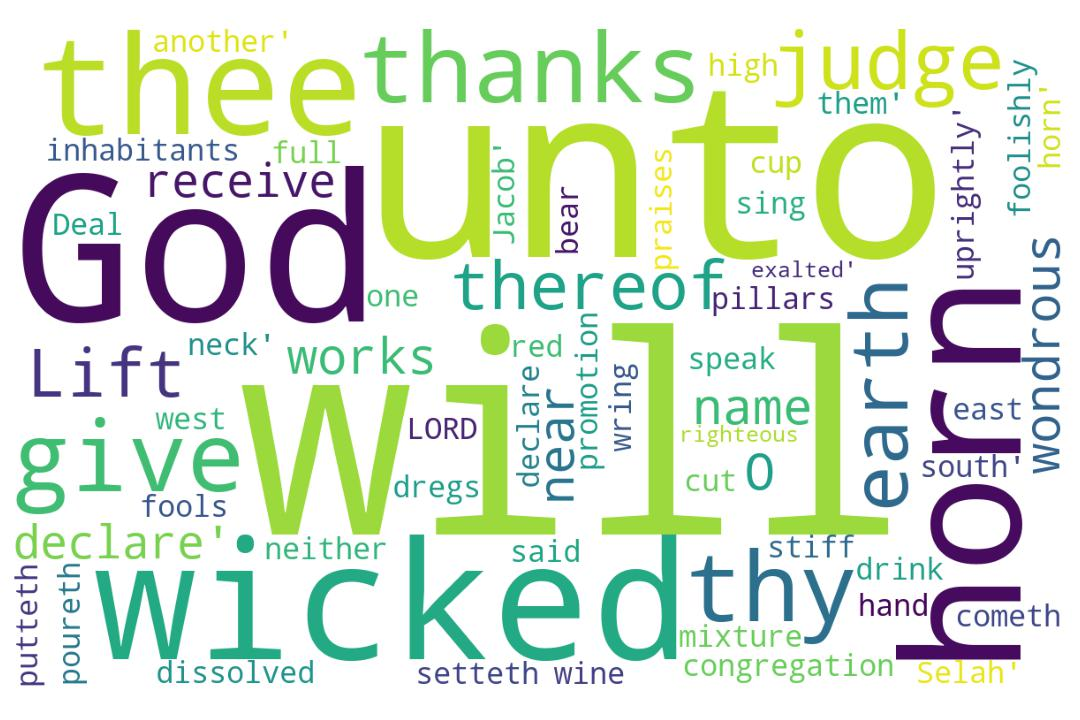
\includegraphics[width=\linewidth]{19OT-Psalms/Psalm75-WordCloud.jpg}
  \caption{Psalm 75 Word Cloud}
  \label{fig:Psalm 75 word Cloud}
\end{figure}

\marginpar{\scriptsize \centering \fcolorbox{bone}{lime}{\textbf{A WORTHY GOD}}\\ (Psalm 75:1-10) \begin{compactenum}[I.][8]
    \item A \textbf{Worthy Declaration} \index[scripture]{Psalms!Psa 075:01}(Psa 75:1)
    \item \textbf{Works on Display} \index[scripture]{Psalms!Psa 075:01}(Psa 75:1)
    \item (Sinful) \textbf{World Dissolved} \index[scripture]{Psalms!Psa 075:03}(Psa 75:3)
    \item \textbf{Weighty Decisions} \index[scripture]{Psalms!Psa 075:07}(Psa 75:7)
     \item A \textbf{Wrathful Drink} (The Cup) \index[scripture]{Psalms!Psa 075:08}(Psa 75:8)
     \item The \textbf{Wringing out of Dregs} \index[scripture]{Psalms!Psa 075:08}(Psa 75:8)
   \item (The) \textbf{Wicked Destroyed} \index[scripture]{Psalms!Psa 075:10}(Psa 75:10)
\end{compactenum}}
    
\marginpar{\scriptsize \centering \fcolorbox{bone}{yellow}{\textbf{THE JUDGMENT}}\\ (Psalm 75:1-10) \begin{compactenum}[I.][8]
    \item The \textbf{Declaration} \index[scripture]{Psalms!Psa 075:01} \index[scripture]{Psalms!Psa 075:09}(Psa 75:1, 9)
    \item \textbf{Dealings} \index[scripture]{Psalms!Psa 075:04} (Psa 75:4)
    \item \textbf{Dissolution} \index[scripture]{Psalms!Psa 075:05} (Psa 75:5)
    \item \textbf{Directions} \index[scripture]{Psalms!Psa 075:06} (Psa 75:6) (Look North!)
    \item \textbf{Dregs} \index[scripture]{Psalms!Psa 075:08} (Psa 75:8) 
    \item The \textbf{Drinking} \index[scripture]{Psalms!Psa 075:08} (Psa 75:8) 
    \item The \textbf{Defeat} \index[scripture]{Psalms!Psa 075:10} (Psa 75:10) 
\end{compactenum}}
    




% \textcolor[cmyk]{0.99998,1,0,0}{
\footnote{\textcolor[rgb]{0.00,0.25,0.00}{\hyperlink{TOC}{Return to end of Table of Contents.}}}\footnote{\href{https://audiobible.com/bible/psalms_75.html}{\textcolor[cmyk]{0.99998,1,0,0}{Psalm 75 Audio}}}\textcolor[cmyk]{0.99998,1,0,0}{To the chief Musician, Al-taschith, A Psalm \emph{or} Song of Asaph.}\\
\\
\textcolor[cmyk]{0.99998,1,0,0}{Unto thee, O God, do we give thanks, \emph{unto} \emph{thee} do we give thanks: for \emph{that} thy name is near thy wondrous \fcolorbox{bone}{lime}{works} declare.}
[2] \textcolor[cmyk]{0.99998,1,0,0}{When I shall receive the congregation I will judge uprightly.}
[3] \textcolor[cmyk]{0.99998,1,0,0}{The earth and all the inhabitants thereof are \fcolorbox{bone}{lime}{dissolved}: I bear up the pillars of it. Selah.}\footnote{\textbf{1 Peter 3:11-12} - Seeing then that all these things shall be dissolved, what manner of persons ought ye to be in all holy conversation and godliness, [12] Looking for and hasting unto the coming of the day of God, wherein the heavens being on fire shall be dissolved, and the elements shall melt with fervent heat?}
[4] \textcolor[cmyk]{0.99998,1,0,0}{I said unto the fools, Deal not foolishly: and to the wicked, Lift not up the horn:}
[5] \textcolor[cmyk]{0.99998,1,0,0}{Lift not up your horn on high: speak \emph{not} \emph{with} a stiff neck.}
[6] \textcolor[cmyk]{0.99998,1,0,0}{For promotion \emph{cometh} neither from the east, nor from the west, nor from the south.}
[7] \textcolor[cmyk]{0.99998,1,0,0}{But God \emph{is} \fcolorbox{bone}{lime}{the judge}: he putteth down one, and setteth up another.}
[8] \textcolor[cmyk]{0.99998,1,0,0}{For in the hand of the LORD \emph{there} \emph{is} a cup, and the wine is red; it is \fcolorbox{bone}{lime}{full of mixture}; and he poureth out of the same: but the dregs thereof, all the wicked of the earth shall \fcolorbox{bone}{lime}{wring} \emph{them} out, \emph{and} drink \emph{them}.}
[9] \textcolor[cmyk]{0.99998,1,0,0}{But I will declare for ever; I will sing praises to the God of Jacob.}
[10] \textcolor[cmyk]{0.99998,1,0,0}{All the horns of the \fcolorbox{bone}{lime}{wicked} also will I cut off; \emph{but} the horns of the righteous shall be exalted.}\footnote{See the horns of \textbf{Revelation 13:1} - And I stood upon the sand of the sea, and saw a beast rise up out of the sea, having seven heads and ten horns, and upon his horns ten crowns, and upon his heads the name of blasphemy. ``Horns'' indicate powers.} 
\index[NWIV]{24!Psalms!Psa 75:1}\index[AWIP]{Unto!Psalms!Psa 75:1}\index[AWIP]{thee!Psalms!Psa 75:1}\index[AWIP]{O!Psalms!Psa 75:1}\index[AWIP]{God!Psalms!Psa 75:1}\index[AWIP]{do!Psalms!Psa 75:1}\index[AWIP]{do!Psalms!Psa 75:1 (2)}\index[AWIP]{we!Psalms!Psa 75:1}\index[AWIP]{we!Psalms!Psa 75:1 (2)}\index[AWIP]{give!Psalms!Psa 75:1}\index[AWIP]{give!Psalms!Psa 75:1 (2)}\index[AWIP]{thanks!Psalms!Psa 75:1}\index[AWIP]{thanks!Psalms!Psa 75:1 (2)}\index[AWIP]{\emph{unto}!Psalms!Psa 75:1}\index[AWIP]{\emph{thee}!Psalms!Psa 75:1}\index[AWIP]{for!Psalms!Psa 75:1}\index[AWIP]{\emph{that}!Psalms!Psa 75:1}\index[AWIP]{thy!Psalms!Psa 75:1}\index[AWIP]{thy!Psalms!Psa 75:1 (2)}\index[AWIP]{name!Psalms!Psa 75:1}\index[AWIP]{is!Psalms!Psa 75:1}\index[AWIP]{near!Psalms!Psa 75:1}\index[AWIP]{wondrous!Psalms!Psa 75:1}\index[AWIP]{works!Psalms!Psa 75:1}\index[AWIP]{declare!Psalms!Psa 75:1}\index[AWIP]{\emph{unto}!Psalms!Psa 75:1}\index[AWIP]{\emph{thee}!Psalms!Psa 75:1}\index[AWIP]{\emph{that}!Psalms!Psa 75:1}

\index[NWIV]{10!Psalms!Psa 75:2}\index[AWIP]{When!Psalms!Psa 75:2}\index[AWIP]{I!Psalms!Psa 75:2}\index[AWIP]{I!Psalms!Psa 75:2 (2)}\index[AWIP]{shall!Psalms!Psa 75:2}\index[AWIP]{receive!Psalms!Psa 75:2}\index[AWIP]{the!Psalms!Psa 75:2}\index[AWIP]{congregation!Psalms!Psa 75:2}\index[AWIP]{will!Psalms!Psa 75:2}\index[AWIP]{judge!Psalms!Psa 75:2}\index[AWIP]{uprightly!Psalms!Psa 75:2}

\index[NWIV]{17!Psalms!Psa 75:3}\index[AWIP]{The!Psalms!Psa 75:3}\index[AWIP]{earth!Psalms!Psa 75:3}\index[AWIP]{and!Psalms!Psa 75:3}\index[AWIP]{all!Psalms!Psa 75:3}\index[AWIP]{the!Psalms!Psa 75:3}\index[AWIP]{the!Psalms!Psa 75:3 (2)}\index[AWIP]{inhabitants!Psalms!Psa 75:3}\index[AWIP]{thereof!Psalms!Psa 75:3}\index[AWIP]{are!Psalms!Psa 75:3}\index[AWIP]{dissolved!Psalms!Psa 75:3}\index[AWIP]{I!Psalms!Psa 75:3}\index[AWIP]{bear!Psalms!Psa 75:3}\index[AWIP]{up!Psalms!Psa 75:3}\index[AWIP]{pillars!Psalms!Psa 75:3}\index[AWIP]{of!Psalms!Psa 75:3}\index[AWIP]{it!Psalms!Psa 75:3}\index[AWIP]{Selah!Psalms!Psa 75:3}

\index[NWIV]{17!Psalms!Psa 75:4}\index[AWIP]{I!Psalms!Psa 75:4}\index[AWIP]{said!Psalms!Psa 75:4}\index[AWIP]{unto!Psalms!Psa 75:4}\index[AWIP]{the!Psalms!Psa 75:4}\index[AWIP]{the!Psalms!Psa 75:4 (2)}\index[AWIP]{the!Psalms!Psa 75:4 (3)}\index[AWIP]{fools!Psalms!Psa 75:4}\index[AWIP]{Deal!Psalms!Psa 75:4}\index[AWIP]{not!Psalms!Psa 75:4}\index[AWIP]{not!Psalms!Psa 75:4 (2)}\index[AWIP]{foolishly!Psalms!Psa 75:4}\index[AWIP]{and!Psalms!Psa 75:4}\index[AWIP]{to!Psalms!Psa 75:4}\index[AWIP]{wicked!Psalms!Psa 75:4}\index[AWIP]{Lift!Psalms!Psa 75:4}\index[AWIP]{up!Psalms!Psa 75:4}\index[AWIP]{horn!Psalms!Psa 75:4}

\index[NWIV]{13!Psalms!Psa 75:5}\index[AWIP]{Lift!Psalms!Psa 75:5}\index[AWIP]{not!Psalms!Psa 75:5}\index[AWIP]{up!Psalms!Psa 75:5}\index[AWIP]{your!Psalms!Psa 75:5}\index[AWIP]{horn!Psalms!Psa 75:5}\index[AWIP]{on!Psalms!Psa 75:5}\index[AWIP]{high!Psalms!Psa 75:5}\index[AWIP]{speak!Psalms!Psa 75:5}\index[AWIP]{\emph{not}!Psalms!Psa 75:5}\index[AWIP]{\emph{with}!Psalms!Psa 75:5}\index[AWIP]{a!Psalms!Psa 75:5}\index[AWIP]{stiff!Psalms!Psa 75:5}\index[AWIP]{neck!Psalms!Psa 75:5}\index[AWIP]{\emph{not}!Psalms!Psa 75:5}\index[AWIP]{\emph{with}!Psalms!Psa 75:5}

\index[NWIV]{15!Psalms!Psa 75:6}\index[AWIP]{For!Psalms!Psa 75:6}\index[AWIP]{promotion!Psalms!Psa 75:6}\index[AWIP]{\emph{cometh}!Psalms!Psa 75:6}\index[AWIP]{neither!Psalms!Psa 75:6}\index[AWIP]{from!Psalms!Psa 75:6}\index[AWIP]{from!Psalms!Psa 75:6 (2)}\index[AWIP]{from!Psalms!Psa 75:6 (3)}\index[AWIP]{the!Psalms!Psa 75:6}\index[AWIP]{the!Psalms!Psa 75:6 (2)}\index[AWIP]{the!Psalms!Psa 75:6 (3)}\index[AWIP]{east!Psalms!Psa 75:6}\index[AWIP]{nor!Psalms!Psa 75:6}\index[AWIP]{nor!Psalms!Psa 75:6 (2)}\index[AWIP]{west!Psalms!Psa 75:6}\index[AWIP]{south!Psalms!Psa 75:6}\index[AWIP]{\emph{cometh}!Psalms!Psa 75:6}

\index[NWIV]{13!Psalms!Psa 75:7}\index[AWIP]{But!Psalms!Psa 75:7}\index[AWIP]{God!Psalms!Psa 75:7}\index[AWIP]{\emph{is}!Psalms!Psa 75:7}\index[AWIP]{the!Psalms!Psa 75:7}\index[AWIP]{judge!Psalms!Psa 75:7}\index[AWIP]{he!Psalms!Psa 75:7}\index[AWIP]{putteth!Psalms!Psa 75:7}\index[AWIP]{down!Psalms!Psa 75:7}\index[AWIP]{one!Psalms!Psa 75:7}\index[AWIP]{and!Psalms!Psa 75:7}\index[AWIP]{setteth!Psalms!Psa 75:7}\index[AWIP]{up!Psalms!Psa 75:7}\index[AWIP]{another!Psalms!Psa 75:7}\index[AWIP]{\emph{is}!Psalms!Psa 75:7}

\index[NWIV]{45!Psalms!Psa 75:8}\index[AWIP]{For!Psalms!Psa 75:8}\index[AWIP]{in!Psalms!Psa 75:8}\index[AWIP]{the!Psalms!Psa 75:8}\index[AWIP]{the!Psalms!Psa 75:8 (2)}\index[AWIP]{the!Psalms!Psa 75:8 (3)}\index[AWIP]{the!Psalms!Psa 75:8 (4)}\index[AWIP]{the!Psalms!Psa 75:8 (5)}\index[AWIP]{the!Psalms!Psa 75:8 (6)}\index[AWIP]{the!Psalms!Psa 75:8 (7)}\index[AWIP]{hand!Psalms!Psa 75:8}\index[AWIP]{of!Psalms!Psa 75:8}\index[AWIP]{of!Psalms!Psa 75:8 (2)}\index[AWIP]{of!Psalms!Psa 75:8 (3)}\index[AWIP]{of!Psalms!Psa 75:8 (4)}\index[AWIP]{LORD!Psalms!Psa 75:8}\index[AWIP]{\emph{there}!Psalms!Psa 75:8}\index[AWIP]{\emph{is}!Psalms!Psa 75:8}\index[AWIP]{a!Psalms!Psa 75:8}\index[AWIP]{cup!Psalms!Psa 75:8}\index[AWIP]{and!Psalms!Psa 75:8}\index[AWIP]{and!Psalms!Psa 75:8 (2)}\index[AWIP]{wine!Psalms!Psa 75:8}\index[AWIP]{is!Psalms!Psa 75:8}\index[AWIP]{is!Psalms!Psa 75:8 (2)}\index[AWIP]{red!Psalms!Psa 75:8}\index[AWIP]{it!Psalms!Psa 75:8}\index[AWIP]{full!Psalms!Psa 75:8}\index[AWIP]{mixture!Psalms!Psa 75:8}\index[AWIP]{he!Psalms!Psa 75:8}\index[AWIP]{poureth!Psalms!Psa 75:8}\index[AWIP]{out!Psalms!Psa 75:8}\index[AWIP]{out!Psalms!Psa 75:8 (2)}\index[AWIP]{same!Psalms!Psa 75:8}\index[AWIP]{but!Psalms!Psa 75:8}\index[AWIP]{dregs!Psalms!Psa 75:8}\index[AWIP]{thereof!Psalms!Psa 75:8}\index[AWIP]{all!Psalms!Psa 75:8}\index[AWIP]{wicked!Psalms!Psa 75:8}\index[AWIP]{earth!Psalms!Psa 75:8}\index[AWIP]{shall!Psalms!Psa 75:8}\index[AWIP]{wring!Psalms!Psa 75:8}\index[AWIP]{\emph{them}!Psalms!Psa 75:8}\index[AWIP]{\emph{them}!Psalms!Psa 75:8 (2)}\index[AWIP]{\emph{and}!Psalms!Psa 75:8}\index[AWIP]{drink!Psalms!Psa 75:8}\index[AWIP]{\emph{there}!Psalms!Psa 75:8}\index[AWIP]{\emph{is}!Psalms!Psa 75:8}\index[AWIP]{\emph{them}!Psalms!Psa 75:8}\index[AWIP]{\emph{them}!Psalms!Psa 75:8 (2)}\index[AWIP]{\emph{and}!Psalms!Psa 75:8}

\index[NWIV]{15!Psalms!Psa 75:9}\index[AWIP]{But!Psalms!Psa 75:9}\index[AWIP]{I!Psalms!Psa 75:9}\index[AWIP]{I!Psalms!Psa 75:9 (2)}\index[AWIP]{will!Psalms!Psa 75:9}\index[AWIP]{will!Psalms!Psa 75:9 (2)}\index[AWIP]{declare!Psalms!Psa 75:9}\index[AWIP]{for!Psalms!Psa 75:9}\index[AWIP]{ever!Psalms!Psa 75:9}\index[AWIP]{sing!Psalms!Psa 75:9}\index[AWIP]{praises!Psalms!Psa 75:9}\index[AWIP]{to!Psalms!Psa 75:9}\index[AWIP]{the!Psalms!Psa 75:9}\index[AWIP]{God!Psalms!Psa 75:9}\index[AWIP]{of!Psalms!Psa 75:9}\index[AWIP]{Jacob!Psalms!Psa 75:9}

\index[NWIV]{20!Psalms!Psa 75:10}\index[AWIP]{All!Psalms!Psa 75:10}\index[AWIP]{the!Psalms!Psa 75:10}\index[AWIP]{the!Psalms!Psa 75:10 (2)}\index[AWIP]{the!Psalms!Psa 75:10 (3)}\index[AWIP]{the!Psalms!Psa 75:10 (4)}\index[AWIP]{horns!Psalms!Psa 75:10}\index[AWIP]{horns!Psalms!Psa 75:10 (2)}\index[AWIP]{of!Psalms!Psa 75:10}\index[AWIP]{of!Psalms!Psa 75:10 (2)}\index[AWIP]{wicked!Psalms!Psa 75:10}\index[AWIP]{also!Psalms!Psa 75:10}\index[AWIP]{will!Psalms!Psa 75:10}\index[AWIP]{I!Psalms!Psa 75:10}\index[AWIP]{cut!Psalms!Psa 75:10}\index[AWIP]{off!Psalms!Psa 75:10}\index[AWIP]{\emph{but}!Psalms!Psa 75:10}\index[AWIP]{righteous!Psalms!Psa 75:10}\index[AWIP]{shall!Psalms!Psa 75:10}\index[AWIP]{be!Psalms!Psa 75:10}\index[AWIP]{exalted!Psalms!Psa 75:10}\index[AWIP]{\emph{but}!Psalms!Psa 75:10}


\section{Psalm 75 Outlines}

\subsection{My Outlines}

\subsubsection{A Worthy God}

\index[speaker]{Keith Anthony!Psalm 075 (A Worthy God)}
\index[series]{Psalms (Keith Anthony)!Psalm 075 (A Worthy God)}
\index[date]{2016/08/19!Psalm 075 (A Worthy God) (Keith Anthony)}

\begin{compactenum}[I.]
    \item A \textbf{Worthy Declaration} \index[scripture]{Psalms!Psa 075:01}(Psa 75:1)
    \item \textbf{Works on Display} \index[scripture]{Psalms!Psa 075:01}(Psa 75:1)
    \item (Sinful) \textbf{World Dissolved} \index[scripture]{Psalms!Psa 075:03}(Psa 75:3)
    \item \textbf{Weight Decisions} \index[scripture]{Psalms!Psa 075:07}(Psa 75:7)
     \item A \textbf{Wrathful Drink} (The Cup) \index[scripture]{Psalms!Psa 075:08}(Psa 75:8)
     \item The \textbf{Wringing out of Dregs} \index[scripture]{Psalms!Psa 075:08}(Psa 75:8)
   \item (The) \textbf{Wicked Destroyed} \index[scripture]{Psalms!Psa 075:10}(Psa 75:10)
\end{compactenum}


\subsubsection{The Judgment}

\index[speaker]{Keith Anthony!Psalm 075 (The Judgment)}
\index[series]{Psalms (Keith Anthony)!Psalm 075 (The Judgment)}
\index[date]{2016/08/19!Psalm 075 (A Worthy God) (The Judgment)}

\begin{compactenum}[I.][8]
    \item The \textbf{Declaration} \index[scripture]{Psalms!Psa 075:01} \index[scripture]{Psalms!Psa 075:09}(Psa 75:1, 9)
    \item \textbf{Dealings} \index[scripture]{Psalms!Psa 075:04} (Psa 75:4)
    \item \textbf{Dissolution} \index[scripture]{Psalms!Psa 075:05} (Psa 75:5)
    \item \textbf{Directions} \index[scripture]{Psalms!Psa 075:06} (Psa 75:6) (Look North!)
    \item \textbf{Dregs} \index[scripture]{Psalms!Psa 075:08} (Psa 75:8) 
    \item The \textbf{Drinking} \index[scripture]{Psalms!Psa 075:08} (Psa 75:8) 
    \item The \textbf{Defeat} \index[scripture]{Psalms!Psa 075:10} (Psa 75:10) 
\end{compactenum}
    

\subsection{Outlines from Others}


\section{Psalm 75 Comments}

\subsection{Numeric Nuggets}
\textbf{13: } Verses 5 and 7 have 13 words. Verses 5, 7, and 9 have 13 unique words.


\subsection{Psalm 75 Repeated Phrases}


%%%%%%%%%%
%%%%%%%%%%
\normalsize
 
\begin{center}
\begin{longtable}{|p{3.0in}|p{0.5in}|}
\caption[Psalm 75 Repeated Phrases]{Psalm 75 Repeated Phrases}\label{table:Repeated Phrases Psalm 75} \\
\hline \multicolumn{1}{|c|}{\textbf{Phrase}} & \multicolumn{1}{c|}{\textbf{Frequency}} \\ \hline 
\endfirsthead
 
\multicolumn{2}{c}
{{\bfseries \tablename\ \thetable{} -- continued from previous page}} \\  
\hline \multicolumn{1}{|c|}{\textbf{Phrase}} & \multicolumn{1}{c|}{\textbf{Frequency}} \\ \hline 
\endhead
 
\hline \multicolumn{2}{c}{{ }} \\ \hline
\endfoot 
of the & 5\\ \hline 
I will & 3\\ \hline 
the wicked & 3\\ \hline 
from the & 3\\ \hline 
\end{longtable}
\end{center}



%%%%%%%%%%
%%%%%%%%%%



\section{Psalm 75 Statistics}

%%%%%%%%%%%%%%%%%%%%%%%%%%%
%%%%% Word Statistics
%%%%%%%%%%%%%%%%%%%%%%%%%%


\normalsize



\subsection{Chapter Word Statistics}


%%%%%%%%%%
%%%%%%%%%%
 
\begin{center}
\begin{longtable}{l|c|c|c|c}
\caption[Stats for Psalm 75]{Stats for Psalm 75} \label{table:Stats for Psalm 75} \\ 
\hline \multicolumn{1}{|c|}{\textbf{Verse(s)}} & \multicolumn{1}{|c|}{\textbf{Count}} & \multicolumn{1}{|c|}{\textbf{Unique}} & \multicolumn{1}{|c|}{\textbf{Italics}} & \multicolumn{1}{|c|}{\textbf{Uniq Italic}}  \\ \hline 
\endfirsthead
 
\multicolumn{5}{c}
{{\bfseries \tablename\ \thetable{} -- continued from previous page}} \\  
\hline \multicolumn{1}{|c|}{\textbf{Verse(s)}} & \multicolumn{1}{|c|}{\textbf{Count}} & \multicolumn{1}{|c|}{\textbf{Unique}} & \multicolumn{1}{|c|}{\textbf{Italics}} & \multicolumn{1}{|c|}{\textbf{Uniq Italic}}  \\ \hline 
\endhead
 
\hline \multicolumn{5}{|r|}{{Continued if needed}} \\ \hline
\endfoot 
1 & 24 & 19 & 3 & 3\\ \hline
2 & 10 & 9 & 0 & 0\\ \hline
3 & 17 & 16 & 0 & 0\\ \hline
4 & 17 & 14 & 0 & 0\\ \hline
5 & 13 & 13 & 2 & 2\\ \hline
6 & 15 & 10 & 1 & 1\\ \hline
7 & 13 & 13 & 1 & 1\\ \hline
8 & 45 & 32 & 5 & 4\\ \hline
9 & 15 & 13 & 0 & 0\\ \hline
10 & 20 & 15 & 1 & 1\\ \hline
\hline \hline
Total & 189 & 109 & 13 & 11



\end{longtable}
\end{center}

%%%%%%%%%%
%%%%%%%%%%
 
\subsection{Words by Frequency}

\begin{center}
\begin{longtable}{l|r}
\caption[Word Frequencies in Psalm 75]{Word Frequencies in Psalm 75} \label{table:WordsIn-Psalm-75} \\ 
\hline \multicolumn{1}{|c|}{\textbf{Word}} & \multicolumn{1}{c|}{\textbf{Frequency}} \\ \hline 
\endfirsthead
 
\multicolumn{2}{c}
{{\bfseries \tablename\ \thetable{} -- continued from previous page}} \\ 
\hline \multicolumn{1}{|c|}{\textbf{Word}} & \multicolumn{1}{c|}{\textbf{Frequency}} \\ \hline 
\endhead
 
\hline \multicolumn{2}{|r|}{{Continued if needed}} \\ \hline
\endfoot
 
\hline \hline
\endlastfoot
the & 22 \\ \hline
of & 8 \\ \hline
I & 7 \\ \hline
and & 5 \\ \hline
will & 4 \\ \hline
up & 4 \\ \hline
God & 3 \\ \hline
is & 3 \\ \hline
shall & 3 \\ \hline
not & 3 \\ \hline
wicked & 3 \\ \hline
from & 3 \\ \hline
do & 2 \\ \hline
we & 2 \\ \hline
give & 2 \\ \hline
thanks & 2 \\ \hline
for & 2 \\ \hline
thy & 2 \\ \hline
declare & 2 \\ \hline
judge & 2 \\ \hline
earth & 2 \\ \hline
all & 2 \\ \hline
thereof & 2 \\ \hline
it & 2 \\ \hline
to & 2 \\ \hline
Lift & 2 \\ \hline
horn & 2 \\ \hline
a & 2 \\ \hline
For & 2 \\ \hline
nor & 2 \\ \hline
But & 2 \\ \hline
\emph{is} & 2 \\ \hline
he & 2 \\ \hline
out & 2 \\ \hline
\emph{them} & 2 \\ \hline
horns & 2 \\ \hline
Unto & 1 \\ \hline
thee & 1 \\ \hline
O & 1 \\ \hline
\emph{unto} & 1 \\ \hline
\emph{thee} & 1 \\ \hline
\emph{that} & 1 \\ \hline
name & 1 \\ \hline
near & 1 \\ \hline
wondrous & 1 \\ \hline
works & 1 \\ \hline
When & 1 \\ \hline
receive & 1 \\ \hline
congregation & 1 \\ \hline
uprightly & 1 \\ \hline
The & 1 \\ \hline
inhabitants & 1 \\ \hline
are & 1 \\ \hline
dissolved & 1 \\ \hline
bear & 1 \\ \hline
pillars & 1 \\ \hline
Selah & 1 \\ \hline
said & 1 \\ \hline
unto & 1 \\ \hline
fools & 1 \\ \hline
Deal & 1 \\ \hline
foolishly & 1 \\ \hline
your & 1 \\ \hline
on & 1 \\ \hline
high & 1 \\ \hline
speak & 1 \\ \hline
\emph{not} & 1 \\ \hline
\emph{with} & 1 \\ \hline
stiff & 1 \\ \hline
neck & 1 \\ \hline
promotion & 1 \\ \hline
\emph{cometh} & 1 \\ \hline
neither & 1 \\ \hline
east & 1 \\ \hline
west & 1 \\ \hline
south & 1 \\ \hline
putteth & 1 \\ \hline
down & 1 \\ \hline
one & 1 \\ \hline
setteth & 1 \\ \hline
another & 1 \\ \hline
in & 1 \\ \hline
hand & 1 \\ \hline
LORD & 1 \\ \hline
\emph{there} & 1 \\ \hline
cup & 1 \\ \hline
wine & 1 \\ \hline
red & 1 \\ \hline
full & 1 \\ \hline
mixture & 1 \\ \hline
poureth & 1 \\ \hline
same & 1 \\ \hline
but & 1 \\ \hline
dregs & 1 \\ \hline
wring & 1 \\ \hline
\emph{and} & 1 \\ \hline
drink & 1 \\ \hline
ever & 1 \\ \hline
sing & 1 \\ \hline
praises & 1 \\ \hline
Jacob & 1 \\ \hline
All & 1 \\ \hline
also & 1 \\ \hline
cut & 1 \\ \hline
off & 1 \\ \hline
\emph{but} & 1 \\ \hline
righteous & 1 \\ \hline
be & 1 \\ \hline
exalted & 1 \\ \hline
\end{longtable}
\end{center}



\normalsize



\subsection{Words Alphabetically}

\begin{center}
\begin{longtable}{l|r}
\caption[Word Alphabetically in Psalm 75]{Word Alphabetically in Psalm 75} \label{table:WordsIn-Psalm-75} \\ 
\hline \multicolumn{1}{|c|}{\textbf{Word}} & \multicolumn{1}{c|}{\textbf{Frequency}} \\ \hline 
\endfirsthead
 
\multicolumn{2}{c}
{{\bfseries \tablename\ \thetable{} -- continued from previous page}} \\ 
\hline \multicolumn{1}{|c|}{\textbf{Word}} & \multicolumn{1}{c|}{\textbf{Frequency}} \\ \hline 
\endhead
 
\hline \multicolumn{2}{|r|}{{Continued if needed}} \\ \hline
\endfoot
 
\hline \hline
\endlastfoot
All & 1 \\ \hline
But & 2 \\ \hline
Deal & 1 \\ \hline
For & 2 \\ \hline
God & 3 \\ \hline
I & 7 \\ \hline
Jacob & 1 \\ \hline
LORD & 1 \\ \hline
Lift & 2 \\ \hline
O & 1 \\ \hline
Selah & 1 \\ \hline
The & 1 \\ \hline
Unto & 1 \\ \hline
When & 1 \\ \hline
\emph{and} & 1 \\ \hline
\emph{but} & 1 \\ \hline
\emph{cometh} & 1 \\ \hline
\emph{is} & 2 \\ \hline
\emph{not} & 1 \\ \hline
\emph{that} & 1 \\ \hline
\emph{thee} & 1 \\ \hline
\emph{them} & 2 \\ \hline
\emph{there} & 1 \\ \hline
\emph{unto} & 1 \\ \hline
\emph{with} & 1 \\ \hline
a & 2 \\ \hline
all & 2 \\ \hline
also & 1 \\ \hline
and & 5 \\ \hline
another & 1 \\ \hline
are & 1 \\ \hline
be & 1 \\ \hline
bear & 1 \\ \hline
but & 1 \\ \hline
congregation & 1 \\ \hline
cup & 1 \\ \hline
cut & 1 \\ \hline
declare & 2 \\ \hline
dissolved & 1 \\ \hline
do & 2 \\ \hline
down & 1 \\ \hline
dregs & 1 \\ \hline
drink & 1 \\ \hline
earth & 2 \\ \hline
east & 1 \\ \hline
ever & 1 \\ \hline
exalted & 1 \\ \hline
foolishly & 1 \\ \hline
fools & 1 \\ \hline
for & 2 \\ \hline
from & 3 \\ \hline
full & 1 \\ \hline
give & 2 \\ \hline
hand & 1 \\ \hline
he & 2 \\ \hline
high & 1 \\ \hline
horn & 2 \\ \hline
horns & 2 \\ \hline
in & 1 \\ \hline
inhabitants & 1 \\ \hline
is & 3 \\ \hline
it & 2 \\ \hline
judge & 2 \\ \hline
mixture & 1 \\ \hline
name & 1 \\ \hline
near & 1 \\ \hline
neck & 1 \\ \hline
neither & 1 \\ \hline
nor & 2 \\ \hline
not & 3 \\ \hline
of & 8 \\ \hline
off & 1 \\ \hline
on & 1 \\ \hline
one & 1 \\ \hline
out & 2 \\ \hline
pillars & 1 \\ \hline
poureth & 1 \\ \hline
praises & 1 \\ \hline
promotion & 1 \\ \hline
putteth & 1 \\ \hline
receive & 1 \\ \hline
red & 1 \\ \hline
righteous & 1 \\ \hline
said & 1 \\ \hline
same & 1 \\ \hline
setteth & 1 \\ \hline
shall & 3 \\ \hline
sing & 1 \\ \hline
south & 1 \\ \hline
speak & 1 \\ \hline
stiff & 1 \\ \hline
thanks & 2 \\ \hline
the & 22 \\ \hline
thee & 1 \\ \hline
thereof & 2 \\ \hline
thy & 2 \\ \hline
to & 2 \\ \hline
unto & 1 \\ \hline
up & 4 \\ \hline
uprightly & 1 \\ \hline
we & 2 \\ \hline
west & 1 \\ \hline
wicked & 3 \\ \hline
will & 4 \\ \hline
wine & 1 \\ \hline
wondrous & 1 \\ \hline
works & 1 \\ \hline
wring & 1 \\ \hline
your & 1 \\ \hline
\end{longtable}
\end{center}



\normalsize



\subsection{Word Lengths in Chapter}
\normalsize
\begin{longtable}{l|p{3.75in}}
\caption[Words by Length in Psalm 75]{Words by Length in Psalm 75} \label{table:WordsIn-Psalm-75} \\ 
\hline \multicolumn{1}{|c|}{\textbf{Length}} & \multicolumn{1}{c|}{\textbf{Words}} \\ \hline 
\endfirsthead
 
\multicolumn{2}{c}
{{\bfseries \tablename\ \thetable{} -- continued from previous page}} \\ 
\hline \multicolumn{1}{|c|}{\textbf{Length}} & \multicolumn{1}{c|}{\textbf{Words}} \\ \hline 
\endhead
 
\hline \multicolumn{2}{|r|}{{Continued if needed}} \\ \hline
\endfoot
 
\hline \hline
\endlastfoot
1 & O, I, a \\ \hline
2 & do, we, is, up, of, it, to, on, \emph{is}, he, in, be \\ \hline
3 & God, for, thy, the, The, and, all, are, not, \emph{not}, For, nor, But, one, cup, red, out, but, \emph{and}, All, cut, off, \emph{but} \\ \hline
4 & Unto, thee, give, \emph{unto}, \emph{thee}, \emph{that}, name, near, When, will, bear, said, unto, Deal, Lift, horn, your, high, \emph{with}, neck, from, east, west, down, hand, LORD, wine, full, same, \emph{them}, ever, sing, also \\ \hline
5 & works, shall, judge, earth, Selah, fools, speak, stiff, south, \emph{there}, dregs, wring, drink, Jacob, horns \\ \hline
6 & thanks, wicked, \emph{cometh} \\ \hline
7 & declare, receive, thereof, pillars, neither, putteth, setteth, another, mixture, poureth, praises, exalted \\ \hline
8 & wondrous \\ \hline
9 & uprightly, dissolved, foolishly, promotion, righteous \\ \hline
11 & inhabitants \\ \hline
12 & congregation \\ \hline
\end{longtable}






%%%%%%%%%%
%%%%%%%%%%
 



%%%%%%%%%%
%%%%%%%%%%
\subsection{Verses with 13 Words in Chapter}
\normalsize
\begin{longtable}{l|p{3.75in}}
\caption[Verses with 13 Words  in Psalm 75]{Verses with 13 Words  in Psalm 75} \label{table:Verses with 13 Words in-Psalm-75} \\ 
\hline \multicolumn{1}{|c|}{\textbf{Reference}} & \multicolumn{1}{c|}{\textbf{Verse}} \\ \hline 
\endfirsthead
 
\multicolumn{2}{c}
{{\bfseries \tablename\ \thetable{} -- continued from previous page}} \\ 
\hline \multicolumn{1}{|c|}{\textbf{Reference}} & \multicolumn{1}{c|}{\textbf{Verse}} \\ \hline 
\endhead
 
\hline \multicolumn{2}{|r|}{{Continued if needed}} \\ \hline
\endfoot
 
\hline \hline
\endlastfoot
Psalms 075:5 & Lift not up your horn on high: speak \emph{not} \emph{with} a stiff neck. \\ \hline
Psalms 075:7 & But God \emph{is} the judge: he putteth down one, and setteth up another. \\ \hline
\end{longtable}






%%%%%%%%%%
%%%%%%%%%%
 

 \chapter{Proverb 16}
 
\begin{figure}
  \includegraphics[width=\linewidth]{20OT-Proverbs/Proverb16-Wordcloud.jpg}
  \caption{Proverb 16 Word Cloud}
  \label{fig:Proverb 16 word Cloud}
\end{figure}

\marginpar{\scriptsize \centering \fcolorbox{bone}{lime}{\textbf{PRAYERS FOR THE FAITHFUL}}\\ (Proverb 16:1-33) \begin{compactenum}[I.][8]
    \item \textbf{Prepare my Heart}  \index[scripture]{Proverbs!Pro 16:01}(Pro 16:1)
    \item \textbf{Peruse my Ways} \index[scripture]{Proverbs!Pro 16:02}(Pro 16:2)
    \item \textbf{Purify my Thoughts} \index[scripture]{Proverbs!Pro 16:03}(Pro 16:3)
    \item \textbf{Point out the Path} \index[scripture]{Proverbs!Pro 16:09}(Pro 16:9)
    \item \textbf{Passify my Anger} \index[scripture]{Proverbs!Pro 16:14}(Pro 16:14)
    \item \textbf{Preserve my Soul} \index[scripture]{Proverbs!Pro 16:17}(Pro 16:17)
    \item \textbf{Impart Wisdom} \index[scripture]{Proverbs!Pro 16:21}(Pro 16:21)
\end{compactenum}}

\marginpar{\scriptsize \centering \fcolorbox{bone}{yellow}{\textbf{A GODLY MAN}}\\ (Proverb 16:1-33) \begin{compactenum}[I.][8]
    \item Is \textbf{Prepared}  \index[scripture]{Proverbs!Pro 16:01} (Pro 16:1)
    \item Is \textbf{Purposed}  \index[scripture]{Proverbs!Pro 16:03} (Pro 16:3)
    \item Has \textbf{Purged} Iniquity  \index[scripture]{Proverbs!Pro 16:06} (Pro 16:6)
    \item Is \textbf{Peaceable}   \index[scripture]{Proverbs!Pro 16:07} (Pro 16:7)
    \item Is \textbf{Preserved}   \index[scripture]{Proverbs!Pro 16:17} (Pro 16:17)
    \item Is not \textbf{Proud}   \index[scripture]{Proverbs!Pro 16:19} (Pro 16:19)
    \item Is \textbf{Prudent}   \index[scripture]{Proverbs!Pro 16:21} (Pro 16:21)
\end{compactenum}}

\marginpar{\scriptsize \centering \fcolorbox{bone}{black}{\textbf{\textcolor[cmyk]{0,0,0,0}{GOD IN CONTROL}}}\\ (Proverb 16) 
 \begin{compactenum}[I.][8]
	\item \textbf{Determined Spirits} \index[scripture]{Proverbs!Pro 16:09} (Pro 16:9)
	\item \textbf{Directed Steps}  \index[scripture]{Proverbs!Pro 16:09} (Pro 16:9)
	\item A \textbf{Divine Sentence}  \index[scripture]{Proverbs!Pro 16:10}  (Pro 16:10)
	\item \textbf{Destroyed Soul}  \index[scripture]{Proverbs!Pro 16:18}  (Pro 16:18)
	\item A \textbf{Delighted Soul}  \index[scripture]{Proverbs!Pro 16:19}  (Pro 16:19)
	\item \textbf{Dug-up Sorrows}  \index[scripture]{Proverbs!Pro 16:27} (Pro 16:27)
	\item A \textbf{Disciplined Spirit}  \index[scripture]{Proverbs!Pro 16:32} (Pro 16:32)
\end{compactenum}}


\marginpar{\scriptsize \centering \fcolorbox{bone}{blue}{\textbf{\textcolor[cmyk]{0,0,0,0}{DETAILS}}}\\ (Proverb 16) 
 \begin{compactenum}[I.][8]

 	\item The \textbf{Works} \index[scripture]{Proverbs!Pro 16:03}(Pro 16:3)
	\item The \textbf{Wicked} \index[scripture]{Proverbs!Pro 16:04}(Pro 16:4)
	\item The \textbf{Ways} \index[scripture]{Proverbs!Pro 16:07}(Pro 16:7)
	\item The \textbf{Way} \index[scripture]{Proverbs!Pro 16:09}\index[scripture]{Proverbs!Pro 16:17}\index[scripture]{Proverbs!Pro 16:25}\index[scripture]{Proverbs!Pro 16:29}\index[scripture]{Proverbs!Pro 16:31}(Pro 16:9, 17, 25, 29, 31)
	\item The \textbf{Weights} \index[scripture]{Proverbs!Pro 16:11}(Pro 16:11)
	\item The \textbf{Wisdom} \index[scripture]{Proverbs!Pro 16:16}(Pro 16:16)
	\item The \textbf{Wellspring} \index[scripture]{Proverbs!Pro 16:22}(Pro 16:22)
	\item The \textbf{Words} \index[scripture]{Proverbs!Pro 16:24}(Pro 16:24)
	\item The \textbf{Whisperer} \index[scripture]{Proverbs!Pro 16:28}(Pro 16:28)
\end{compactenum}}








\footnote{\textcolor[cmyk]{0.99998,1,0,0}{\hyperlink{TOC}{Return to end of Table of Contents.}}}\footnote{\href{https://audiobible.com/bible/proverbs_16.html}{\textcolor[cmyk]{0.99998,1,0,0}{Proverbs Audio}}}\textcolor[cmyk]{0.99998,1,0,0}{The \fcolorbox{bone}{lime}{preparations of the heart} in man, and the answer of the tongue, \emph{is} from the LORD.}
[2] \textcolor[cmyk]{0.99998,1,0,0}{All the ways of a man \emph{are} clean in his own eyes; but the \fcolorbox{bone}{lime}{LORD} \fcolorbox{bone}{lime}{weigheth} \fcolorbox{bone}{lime}{the} \fcolorbox{bone}{lime}{spirits}.}
[3] \textcolor[cmyk]{0.99998,1,0,0}{Commit thy works unto the LORD, and thy \fcolorbox{bone}{lime}{thoughts shall be} \fcolorbox{bone}{lime}{established}.}
[4] \textcolor[cmyk]{0.99998,1,0,0}{The LORD hath made all \emph{things} for himself: yea, even the wicked for the day of evil.}
[5] \textcolor[cmyk]{0.99998,1,0,0}{Every one \emph{that} \emph{is} proud in heart \emph{is} an abomination to the LORD: \emph{though} hand \emph{join} in hand, he shall not be unpunished.}
[6] \textcolor[cmyk]{0.99998,1,0,0}{By mercy and truth iniquity is purged: and by the fear of the LORD \emph{men} depart from evil.}
[7] \textcolor[cmyk]{0.99998,1,0,0}{When a man's ways please the LORD, he maketh even his enemies to be at peace with him.}
[8] \textcolor[cmyk]{0.99998,1,0,0}{Better \emph{is} a little with \fcolorbox{bone}{MYGOLD}{righteousness} than great revenues without right.}
[9] \textcolor[cmyk]{0.99998,1,0,0}{A man's heart deviseth his way: but the \fcolorbox{bone}{lime}{LORD directeth his steps}.}
[10] \textcolor[cmyk]{0.99998,1,0,0}{A divine sentence \emph{is} in the lips of the king: his mouth \fcolorbox{bone}{MYGOLD}{transgresseth} not in judgment.}
[11] \textcolor[cmyk]{0.99998,1,0,0}{A just weight and balance \emph{are} the LORD'S: all the weights of the bag \emph{are} his work.}
[12] \textcolor[cmyk]{0.99998,1,0,0}{\emph{It} \emph{is} an abomination to kings to commit wickedness: for the throne is established by \fcolorbox{bone}{MYGOLD}{righteousness}.}
[13] \textcolor[cmyk]{0.99998,1,0,0}{Righteous lips \emph{are} the delight of kings; and they love him that speaketh right.}
[14] \textcolor[cmyk]{0.99998,1,0,0}{The wrath of a king \emph{is} \emph{as} messengers of death: but a \fcolorbox{bone}{lime}{wise man will pacify it}.}
[15] \textcolor[cmyk]{0.99998,1,0,0}{In the light of the king's countenance \emph{is} life; and his favour \emph{is} as a cloud of the latter rain.}
[16] \textcolor[cmyk]{0.99998,1,0,0}{How much better \emph{is} \emph{it} to get wisdom than gold! and to get \fcolorbox{bone}{MYGOLD}{understanding} rather to be chosen than silver!}
[17] \textcolor[cmyk]{0.99998,1,0,0}{The highway of the upright \emph{is} to depart from evil: he that keepeth his way \fcolorbox{bone}{lime}{preserveth} his soul.}
[18] \textcolor[cmyk]{0.99998,1,0,0}{Pride \emph{goeth} before destruction, and an haughty spirit before a fall.}
[19] \textcolor[cmyk]{0.99998,1,0,0}{Better \emph{it} \emph{is} \emph{to} \emph{be} of an humble spirit with the lowly, than to divide the spoil with the proud.}
[20] \textcolor[cmyk]{0.99998,1,0,0}{He that handleth a matter wisely shall find good: and whoso trusteth in the LORD, happy \emph{is} he.}
[21] \textcolor[cmyk]{0.99998,1,0,0}{The \fcolorbox{bone}{lime}{wise in heart} shall be called prudent: and the sweetness of the lips increaseth learning.}
[22] \textcolor[cmyk]{0.99998,1,0,0}{\fcolorbox{bone}{MYGOLD}{Understanding} \emph{is} a wellspring of life unto him that hath it: but the instruction of fools \emph{is} folly.}\footnote{\textbf{Proverbs 18:4} - The words of a man’s mouth are as deep waters, and the wellspring of wisdom as a flowing brook.}\marginpar{ \scriptsize  {\textcolor[rgb]{0.00,0.545,0.269}{$\rightarrow$``wellspring'' found ONLY here and in Proverbs 18:4.}}}
[23] \textcolor[cmyk]{0.99998,1,0,0}{The heart of the wise teacheth his mouth, and addeth learning to his lips.}
[24] \textcolor[cmyk]{0.99998,1,0,0}{Pleasant words \emph{are} \emph{as} an honeycomb, sweet to the soul, and health to the bones.}
[25] \textcolor[cmyk]{0.99998,1,0,0}{There is a way that seemeth right unto a man, but the end thereof \emph{are} the ways of death.}
[26] \textcolor[cmyk]{0.99998,1,0,0}{He that laboureth laboureth for himself; for his mouth craveth it of him.}
[27] \textcolor[cmyk]{0.99998,1,0,0}{An ungodly man diggeth up evil: and in his lips \emph{there} \emph{is} as a burning fire.}
[28] \textcolor[cmyk]{0.99998,1,0,0}{A froward man soweth strife: and a whisperer separateth chief friends.}\footnote{\textbf{Proverb 6:14} - Frowardness is in his heart, he deviseth mischief continually; he soweth discord.}\footnote{\textbf{Proverb 6:19} - A false witness that speaketh lies, and he that soweth discord among brethren.}
[29] \textcolor[cmyk]{0.99998,1,0,0}{A violent man enticeth his neighbour, and leadeth him into the way \emph{that} \emph{is} not good.}
[30] \textcolor[cmyk]{0.99998,1,0,0}{He shutteth his eyes to devise froward things: moving his lips he bringeth evil to pass.}
[31] \textcolor[cmyk]{0.99998,1,0,0}{The hoary head \emph{is} a crown of glory, \emph{if} it be found in the way of \fcolorbox{bone}{MYGOLD}{righteousness}.}
[32] \textcolor[cmyk]{0.99998,1,0,0}{\emph{He} \emph{that} \emph{is} slow to anger \emph{is} better than the mighty; and he that ruleth his spirit than he that taketh a city.}
[33] \textcolor[cmyk]{0.99998,1,0,0}{The lot is cast into the lap; but the whole disposing thereof \emph{is} of the LORD.}



\index[NWIV]{17!Proverbs!Pro 16:1}\index[AWIP]{The!Proverbs!Pro 16:1}\index[AWIP]{preparations!Proverbs!Pro 16:1}\index[AWIP]{of!Proverbs!Pro 16:1}\index[AWIP]{of!Proverbs!Pro 16:1 (2)}\index[AWIP]{the!Proverbs!Pro 16:1}\index[AWIP]{the!Proverbs!Pro 16:1 (2)}\index[AWIP]{the!Proverbs!Pro 16:1 (3)}\index[AWIP]{the!Proverbs!Pro 16:1 (4)}\index[AWIP]{heart!Proverbs!Pro 16:1}\index[AWIP]{in!Proverbs!Pro 16:1}\index[AWIP]{man!Proverbs!Pro 16:1}\index[AWIP]{and!Proverbs!Pro 16:1}\index[AWIP]{answer!Proverbs!Pro 16:1}\index[AWIP]{tongue!Proverbs!Pro 16:1}\index[AWIP]{\emph{is}!Proverbs!Pro 16:1}\index[AWIP]{from!Proverbs!Pro 16:1}\index[AWIP]{LORD!Proverbs!Pro 16:1}\index[AWIP]{\emph{is}!Proverbs!Pro 16:1}

\index[NWIV]{18!Proverbs!Pro 16:2}\index[AWIP]{All!Proverbs!Pro 16:2}\index[AWIP]{the!Proverbs!Pro 16:2}\index[AWIP]{the!Proverbs!Pro 16:2 (2)}\index[AWIP]{the!Proverbs!Pro 16:2 (3)}\index[AWIP]{ways!Proverbs!Pro 16:2}\index[AWIP]{of!Proverbs!Pro 16:2}\index[AWIP]{a!Proverbs!Pro 16:2}\index[AWIP]{man!Proverbs!Pro 16:2}\index[AWIP]{\emph{are}!Proverbs!Pro 16:2}\index[AWIP]{clean!Proverbs!Pro 16:2}\index[AWIP]{in!Proverbs!Pro 16:2}\index[AWIP]{his!Proverbs!Pro 16:2}\index[AWIP]{own!Proverbs!Pro 16:2}\index[AWIP]{eyes!Proverbs!Pro 16:2}\index[AWIP]{but!Proverbs!Pro 16:2}\index[AWIP]{LORD!Proverbs!Pro 16:2}\index[AWIP]{weigheth!Proverbs!Pro 16:2}\index[AWIP]{spirits!Proverbs!Pro 16:2}\index[AWIP]{\emph{are}!Proverbs!Pro 16:2}

\index[NWIV]{12!Proverbs!Pro 16:3}\index[AWIP]{Commit!Proverbs!Pro 16:3}\index[AWIP]{thy!Proverbs!Pro 16:3}\index[AWIP]{thy!Proverbs!Pro 16:3 (2)}\index[AWIP]{works!Proverbs!Pro 16:3}\index[AWIP]{unto!Proverbs!Pro 16:3}\index[AWIP]{the!Proverbs!Pro 16:3}\index[AWIP]{LORD!Proverbs!Pro 16:3}\index[AWIP]{and!Proverbs!Pro 16:3}\index[AWIP]{thoughts!Proverbs!Pro 16:3}\index[AWIP]{shall!Proverbs!Pro 16:3}\index[AWIP]{be!Proverbs!Pro 16:3}\index[AWIP]{established!Proverbs!Pro 16:3}

\index[NWIV]{17!Proverbs!Pro 16:4}\index[AWIP]{The!Proverbs!Pro 16:4}\index[AWIP]{LORD!Proverbs!Pro 16:4}\index[AWIP]{hath!Proverbs!Pro 16:4}\index[AWIP]{made!Proverbs!Pro 16:4}\index[AWIP]{all!Proverbs!Pro 16:4}\index[AWIP]{\emph{things}!Proverbs!Pro 16:4}\index[AWIP]{for!Proverbs!Pro 16:4}\index[AWIP]{for!Proverbs!Pro 16:4 (2)}\index[AWIP]{himself!Proverbs!Pro 16:4}\index[AWIP]{yea!Proverbs!Pro 16:4}\index[AWIP]{even!Proverbs!Pro 16:4}\index[AWIP]{the!Proverbs!Pro 16:4}\index[AWIP]{the!Proverbs!Pro 16:4 (2)}\index[AWIP]{wicked!Proverbs!Pro 16:4}\index[AWIP]{day!Proverbs!Pro 16:4}\index[AWIP]{of!Proverbs!Pro 16:4}\index[AWIP]{evil!Proverbs!Pro 16:4}\index[AWIP]{\emph{things}!Proverbs!Pro 16:4}

\index[NWIV]{23!Proverbs!Pro 16:5}\index[AWIP]{Every!Proverbs!Pro 16:5}\index[AWIP]{one!Proverbs!Pro 16:5}\index[AWIP]{\emph{that}!Proverbs!Pro 16:5}\index[AWIP]{\emph{is}!Proverbs!Pro 16:5}\index[AWIP]{\emph{is}!Proverbs!Pro 16:5 (2)}\index[AWIP]{proud!Proverbs!Pro 16:5}\index[AWIP]{in!Proverbs!Pro 16:5}\index[AWIP]{in!Proverbs!Pro 16:5 (2)}\index[AWIP]{heart!Proverbs!Pro 16:5}\index[AWIP]{an!Proverbs!Pro 16:5}\index[AWIP]{abomination!Proverbs!Pro 16:5}\index[AWIP]{to!Proverbs!Pro 16:5}\index[AWIP]{the!Proverbs!Pro 16:5}\index[AWIP]{LORD!Proverbs!Pro 16:5}\index[AWIP]{\emph{though}!Proverbs!Pro 16:5}\index[AWIP]{hand!Proverbs!Pro 16:5}\index[AWIP]{hand!Proverbs!Pro 16:5 (2)}\index[AWIP]{\emph{join}!Proverbs!Pro 16:5}\index[AWIP]{he!Proverbs!Pro 16:5}\index[AWIP]{shall!Proverbs!Pro 16:5}\index[AWIP]{not!Proverbs!Pro 16:5}\index[AWIP]{be!Proverbs!Pro 16:5}\index[AWIP]{unpunished!Proverbs!Pro 16:5}\index[AWIP]{\emph{that}!Proverbs!Pro 16:5}\index[AWIP]{\emph{is}!Proverbs!Pro 16:5}\index[AWIP]{\emph{is}!Proverbs!Pro 16:5 (2)}\index[AWIP]{\emph{though}!Proverbs!Pro 16:5}\index[AWIP]{\emph{join}!Proverbs!Pro 16:5}

\index[NWIV]{18!Proverbs!Pro 16:6}\index[AWIP]{By!Proverbs!Pro 16:6}\index[AWIP]{mercy!Proverbs!Pro 16:6}\index[AWIP]{and!Proverbs!Pro 16:6}\index[AWIP]{and!Proverbs!Pro 16:6 (2)}\index[AWIP]{truth!Proverbs!Pro 16:6}\index[AWIP]{iniquity!Proverbs!Pro 16:6}\index[AWIP]{is!Proverbs!Pro 16:6}\index[AWIP]{purged!Proverbs!Pro 16:6}\index[AWIP]{by!Proverbs!Pro 16:6}\index[AWIP]{the!Proverbs!Pro 16:6}\index[AWIP]{the!Proverbs!Pro 16:6 (2)}\index[AWIP]{fear!Proverbs!Pro 16:6}\index[AWIP]{of!Proverbs!Pro 16:6}\index[AWIP]{LORD!Proverbs!Pro 16:6}\index[AWIP]{\emph{men}!Proverbs!Pro 16:6}\index[AWIP]{depart!Proverbs!Pro 16:6}\index[AWIP]{from!Proverbs!Pro 16:6}\index[AWIP]{evil!Proverbs!Pro 16:6}\index[AWIP]{\emph{men}!Proverbs!Pro 16:6}

\index[NWIV]{18!Proverbs!Pro 16:7}\index[AWIP]{When!Proverbs!Pro 16:7}\index[AWIP]{a!Proverbs!Pro 16:7}\index[AWIP]{man's!Proverbs!Pro 16:7}\index[AWIP]{ways!Proverbs!Pro 16:7}\index[AWIP]{please!Proverbs!Pro 16:7}\index[AWIP]{the!Proverbs!Pro 16:7}\index[AWIP]{LORD!Proverbs!Pro 16:7}\index[AWIP]{he!Proverbs!Pro 16:7}\index[AWIP]{maketh!Proverbs!Pro 16:7}\index[AWIP]{even!Proverbs!Pro 16:7}\index[AWIP]{his!Proverbs!Pro 16:7}\index[AWIP]{enemies!Proverbs!Pro 16:7}\index[AWIP]{to!Proverbs!Pro 16:7}\index[AWIP]{be!Proverbs!Pro 16:7}\index[AWIP]{at!Proverbs!Pro 16:7}\index[AWIP]{peace!Proverbs!Pro 16:7}\index[AWIP]{with!Proverbs!Pro 16:7}\index[AWIP]{him!Proverbs!Pro 16:7}

\index[NWIV]{11!Proverbs!Pro 16:8}\index[AWIP]{Better!Proverbs!Pro 16:8}\index[AWIP]{\emph{is}!Proverbs!Pro 16:8}\index[AWIP]{a!Proverbs!Pro 16:8}\index[AWIP]{little!Proverbs!Pro 16:8}\index[AWIP]{with!Proverbs!Pro 16:8}\index[AWIP]{righteousness!Proverbs!Pro 16:8}\index[AWIP]{than!Proverbs!Pro 16:8}\index[AWIP]{great!Proverbs!Pro 16:8}\index[AWIP]{revenues!Proverbs!Pro 16:8}\index[AWIP]{without!Proverbs!Pro 16:8}\index[AWIP]{right!Proverbs!Pro 16:8}\index[AWIP]{\emph{is}!Proverbs!Pro 16:8}

\index[NWIV]{12!Proverbs!Pro 16:9}\index[AWIP]{A!Proverbs!Pro 16:9}\index[AWIP]{man's!Proverbs!Pro 16:9}\index[AWIP]{heart!Proverbs!Pro 16:9}\index[AWIP]{deviseth!Proverbs!Pro 16:9}\index[AWIP]{his!Proverbs!Pro 16:9}\index[AWIP]{his!Proverbs!Pro 16:9 (2)}\index[AWIP]{way!Proverbs!Pro 16:9}\index[AWIP]{but!Proverbs!Pro 16:9}\index[AWIP]{the!Proverbs!Pro 16:9}\index[AWIP]{LORD!Proverbs!Pro 16:9}\index[AWIP]{directeth!Proverbs!Pro 16:9}\index[AWIP]{steps!Proverbs!Pro 16:9}

\index[NWIV]{16!Proverbs!Pro 16:10}\index[AWIP]{A!Proverbs!Pro 16:10}\index[AWIP]{divine!Proverbs!Pro 16:10}\index[AWIP]{sentence!Proverbs!Pro 16:10}\index[AWIP]{\emph{is}!Proverbs!Pro 16:10}\index[AWIP]{in!Proverbs!Pro 16:10}\index[AWIP]{in!Proverbs!Pro 16:10 (2)}\index[AWIP]{the!Proverbs!Pro 16:10}\index[AWIP]{the!Proverbs!Pro 16:10 (2)}\index[AWIP]{lips!Proverbs!Pro 16:10}\index[AWIP]{of!Proverbs!Pro 16:10}\index[AWIP]{king!Proverbs!Pro 16:10}\index[AWIP]{his!Proverbs!Pro 16:10}\index[AWIP]{mouth!Proverbs!Pro 16:10}\index[AWIP]{transgresseth!Proverbs!Pro 16:10}\index[AWIP]{not!Proverbs!Pro 16:10}\index[AWIP]{judgment!Proverbs!Pro 16:10}\index[AWIP]{\emph{is}!Proverbs!Pro 16:10}

\index[NWIV]{17!Proverbs!Pro 16:11}\index[AWIP]{A!Proverbs!Pro 16:11}\index[AWIP]{just!Proverbs!Pro 16:11}\index[AWIP]{weight!Proverbs!Pro 16:11}\index[AWIP]{and!Proverbs!Pro 16:11}\index[AWIP]{balance!Proverbs!Pro 16:11}\index[AWIP]{\emph{are}!Proverbs!Pro 16:11}\index[AWIP]{\emph{are}!Proverbs!Pro 16:11 (2)}\index[AWIP]{the!Proverbs!Pro 16:11}\index[AWIP]{the!Proverbs!Pro 16:11 (2)}\index[AWIP]{the!Proverbs!Pro 16:11 (3)}\index[AWIP]{LORD'S!Proverbs!Pro 16:11}\index[AWIP]{all!Proverbs!Pro 16:11}\index[AWIP]{weights!Proverbs!Pro 16:11}\index[AWIP]{of!Proverbs!Pro 16:11}\index[AWIP]{bag!Proverbs!Pro 16:11}\index[AWIP]{his!Proverbs!Pro 16:11}\index[AWIP]{work!Proverbs!Pro 16:11}\index[AWIP]{\emph{are}!Proverbs!Pro 16:11}\index[AWIP]{\emph{are}!Proverbs!Pro 16:11 (2)}

\index[NWIV]{16!Proverbs!Pro 16:12}\index[AWIP]{\emph{It}!Proverbs!Pro 16:12}\index[AWIP]{\emph{is}!Proverbs!Pro 16:12}\index[AWIP]{an!Proverbs!Pro 16:12}\index[AWIP]{abomination!Proverbs!Pro 16:12}\index[AWIP]{to!Proverbs!Pro 16:12}\index[AWIP]{to!Proverbs!Pro 16:12 (2)}\index[AWIP]{kings!Proverbs!Pro 16:12}\index[AWIP]{commit!Proverbs!Pro 16:12}\index[AWIP]{wickedness!Proverbs!Pro 16:12}\index[AWIP]{for!Proverbs!Pro 16:12}\index[AWIP]{the!Proverbs!Pro 16:12}\index[AWIP]{throne!Proverbs!Pro 16:12}\index[AWIP]{is!Proverbs!Pro 16:12}\index[AWIP]{established!Proverbs!Pro 16:12}\index[AWIP]{by!Proverbs!Pro 16:12}\index[AWIP]{righteousness!Proverbs!Pro 16:12}\index[AWIP]{\emph{It}!Proverbs!Pro 16:12}\index[AWIP]{\emph{is}!Proverbs!Pro 16:12}

\index[NWIV]{14!Proverbs!Pro 16:13}\index[AWIP]{Righteous!Proverbs!Pro 16:13}\index[AWIP]{lips!Proverbs!Pro 16:13}\index[AWIP]{\emph{are}!Proverbs!Pro 16:13}\index[AWIP]{the!Proverbs!Pro 16:13}\index[AWIP]{delight!Proverbs!Pro 16:13}\index[AWIP]{of!Proverbs!Pro 16:13}\index[AWIP]{kings!Proverbs!Pro 16:13}\index[AWIP]{and!Proverbs!Pro 16:13}\index[AWIP]{they!Proverbs!Pro 16:13}\index[AWIP]{love!Proverbs!Pro 16:13}\index[AWIP]{him!Proverbs!Pro 16:13}\index[AWIP]{that!Proverbs!Pro 16:13}\index[AWIP]{speaketh!Proverbs!Pro 16:13}\index[AWIP]{right!Proverbs!Pro 16:13}\index[AWIP]{\emph{are}!Proverbs!Pro 16:13}

\index[NWIV]{17!Proverbs!Pro 16:14}\index[AWIP]{The!Proverbs!Pro 16:14}\index[AWIP]{wrath!Proverbs!Pro 16:14}\index[AWIP]{of!Proverbs!Pro 16:14}\index[AWIP]{of!Proverbs!Pro 16:14 (2)}\index[AWIP]{a!Proverbs!Pro 16:14}\index[AWIP]{a!Proverbs!Pro 16:14 (2)}\index[AWIP]{king!Proverbs!Pro 16:14}\index[AWIP]{\emph{is}!Proverbs!Pro 16:14}\index[AWIP]{\emph{as}!Proverbs!Pro 16:14}\index[AWIP]{messengers!Proverbs!Pro 16:14}\index[AWIP]{death!Proverbs!Pro 16:14}\index[AWIP]{but!Proverbs!Pro 16:14}\index[AWIP]{wise!Proverbs!Pro 16:14}\index[AWIP]{man!Proverbs!Pro 16:14}\index[AWIP]{will!Proverbs!Pro 16:14}\index[AWIP]{pacify!Proverbs!Pro 16:14}\index[AWIP]{it!Proverbs!Pro 16:14}\index[AWIP]{\emph{is}!Proverbs!Pro 16:14}\index[AWIP]{\emph{as}!Proverbs!Pro 16:14}

\index[NWIV]{20!Proverbs!Pro 16:15}\index[AWIP]{In!Proverbs!Pro 16:15}\index[AWIP]{the!Proverbs!Pro 16:15}\index[AWIP]{the!Proverbs!Pro 16:15 (2)}\index[AWIP]{the!Proverbs!Pro 16:15 (3)}\index[AWIP]{light!Proverbs!Pro 16:15}\index[AWIP]{of!Proverbs!Pro 16:15}\index[AWIP]{of!Proverbs!Pro 16:15 (2)}\index[AWIP]{king's!Proverbs!Pro 16:15}\index[AWIP]{countenance!Proverbs!Pro 16:15}\index[AWIP]{\emph{is}!Proverbs!Pro 16:15}\index[AWIP]{\emph{is}!Proverbs!Pro 16:15 (2)}\index[AWIP]{life!Proverbs!Pro 16:15}\index[AWIP]{and!Proverbs!Pro 16:15}\index[AWIP]{his!Proverbs!Pro 16:15}\index[AWIP]{favour!Proverbs!Pro 16:15}\index[AWIP]{as!Proverbs!Pro 16:15}\index[AWIP]{a!Proverbs!Pro 16:15}\index[AWIP]{cloud!Proverbs!Pro 16:15}\index[AWIP]{latter!Proverbs!Pro 16:15}\index[AWIP]{rain!Proverbs!Pro 16:15}\index[AWIP]{\emph{is}!Proverbs!Pro 16:15}\index[AWIP]{\emph{is}!Proverbs!Pro 16:15 (2)}

\index[NWIV]{20!Proverbs!Pro 16:16}\index[AWIP]{How!Proverbs!Pro 16:16}\index[AWIP]{much!Proverbs!Pro 16:16}\index[AWIP]{better!Proverbs!Pro 16:16}\index[AWIP]{\emph{is}!Proverbs!Pro 16:16}\index[AWIP]{\emph{it}!Proverbs!Pro 16:16}\index[AWIP]{to!Proverbs!Pro 16:16}\index[AWIP]{to!Proverbs!Pro 16:16 (2)}\index[AWIP]{to!Proverbs!Pro 16:16 (3)}\index[AWIP]{get!Proverbs!Pro 16:16}\index[AWIP]{get!Proverbs!Pro 16:16 (2)}\index[AWIP]{wisdom!Proverbs!Pro 16:16}\index[AWIP]{than!Proverbs!Pro 16:16}\index[AWIP]{than!Proverbs!Pro 16:16 (2)}\index[AWIP]{gold!!Proverbs!Pro 16:16}\index[AWIP]{and!Proverbs!Pro 16:16}\index[AWIP]{understanding!Proverbs!Pro 16:16}\index[AWIP]{rather!Proverbs!Pro 16:16}\index[AWIP]{be!Proverbs!Pro 16:16}\index[AWIP]{chosen!Proverbs!Pro 16:16}\index[AWIP]{silver!!Proverbs!Pro 16:16}\index[AWIP]{\emph{is}!Proverbs!Pro 16:16}\index[AWIP]{\emph{it}!Proverbs!Pro 16:16}

\index[NWIV]{18!Proverbs!Pro 16:17}\index[AWIP]{The!Proverbs!Pro 16:17}\index[AWIP]{highway!Proverbs!Pro 16:17}\index[AWIP]{of!Proverbs!Pro 16:17}\index[AWIP]{the!Proverbs!Pro 16:17}\index[AWIP]{upright!Proverbs!Pro 16:17}\index[AWIP]{\emph{is}!Proverbs!Pro 16:17}\index[AWIP]{to!Proverbs!Pro 16:17}\index[AWIP]{depart!Proverbs!Pro 16:17}\index[AWIP]{from!Proverbs!Pro 16:17}\index[AWIP]{evil!Proverbs!Pro 16:17}\index[AWIP]{he!Proverbs!Pro 16:17}\index[AWIP]{that!Proverbs!Pro 16:17}\index[AWIP]{keepeth!Proverbs!Pro 16:17}\index[AWIP]{his!Proverbs!Pro 16:17}\index[AWIP]{his!Proverbs!Pro 16:17 (2)}\index[AWIP]{way!Proverbs!Pro 16:17}\index[AWIP]{preserveth!Proverbs!Pro 16:17}\index[AWIP]{soul!Proverbs!Pro 16:17}\index[AWIP]{\emph{is}!Proverbs!Pro 16:17}

\index[NWIV]{11!Proverbs!Pro 16:18}\index[AWIP]{Pride!Proverbs!Pro 16:18}\index[AWIP]{\emph{goeth}!Proverbs!Pro 16:18}\index[AWIP]{before!Proverbs!Pro 16:18}\index[AWIP]{before!Proverbs!Pro 16:18 (2)}\index[AWIP]{destruction!Proverbs!Pro 16:18}\index[AWIP]{and!Proverbs!Pro 16:18}\index[AWIP]{an!Proverbs!Pro 16:18}\index[AWIP]{haughty!Proverbs!Pro 16:18}\index[AWIP]{spirit!Proverbs!Pro 16:18}\index[AWIP]{a!Proverbs!Pro 16:18}\index[AWIP]{fall!Proverbs!Pro 16:18}\index[AWIP]{\emph{goeth}!Proverbs!Pro 16:18}

\index[NWIV]{20!Proverbs!Pro 16:19}\index[AWIP]{Better!Proverbs!Pro 16:19}\index[AWIP]{\emph{it}!Proverbs!Pro 16:19}\index[AWIP]{\emph{is}!Proverbs!Pro 16:19}\index[AWIP]{\emph{to}!Proverbs!Pro 16:19}\index[AWIP]{\emph{be}!Proverbs!Pro 16:19}\index[AWIP]{of!Proverbs!Pro 16:19}\index[AWIP]{an!Proverbs!Pro 16:19}\index[AWIP]{humble!Proverbs!Pro 16:19}\index[AWIP]{spirit!Proverbs!Pro 16:19}\index[AWIP]{with!Proverbs!Pro 16:19}\index[AWIP]{with!Proverbs!Pro 16:19 (2)}\index[AWIP]{the!Proverbs!Pro 16:19}\index[AWIP]{the!Proverbs!Pro 16:19 (2)}\index[AWIP]{the!Proverbs!Pro 16:19 (3)}\index[AWIP]{lowly!Proverbs!Pro 16:19}\index[AWIP]{than!Proverbs!Pro 16:19}\index[AWIP]{to!Proverbs!Pro 16:19}\index[AWIP]{divide!Proverbs!Pro 16:19}\index[AWIP]{spoil!Proverbs!Pro 16:19}\index[AWIP]{proud!Proverbs!Pro 16:19}\index[AWIP]{\emph{it}!Proverbs!Pro 16:19}\index[AWIP]{\emph{is}!Proverbs!Pro 16:19}\index[AWIP]{\emph{to}!Proverbs!Pro 16:19}\index[AWIP]{\emph{be}!Proverbs!Pro 16:19}

\index[NWIV]{18!Proverbs!Pro 16:20}\index[AWIP]{He!Proverbs!Pro 16:20}\index[AWIP]{that!Proverbs!Pro 16:20}\index[AWIP]{handleth!Proverbs!Pro 16:20}\index[AWIP]{a!Proverbs!Pro 16:20}\index[AWIP]{matter!Proverbs!Pro 16:20}\index[AWIP]{wisely!Proverbs!Pro 16:20}\index[AWIP]{shall!Proverbs!Pro 16:20}\index[AWIP]{find!Proverbs!Pro 16:20}\index[AWIP]{good!Proverbs!Pro 16:20}\index[AWIP]{and!Proverbs!Pro 16:20}\index[AWIP]{whoso!Proverbs!Pro 16:20}\index[AWIP]{trusteth!Proverbs!Pro 16:20}\index[AWIP]{in!Proverbs!Pro 16:20}\index[AWIP]{the!Proverbs!Pro 16:20}\index[AWIP]{LORD!Proverbs!Pro 16:20}\index[AWIP]{happy!Proverbs!Pro 16:20}\index[AWIP]{\emph{is}!Proverbs!Pro 16:20}\index[AWIP]{he!Proverbs!Pro 16:20}\index[AWIP]{\emph{is}!Proverbs!Pro 16:20}

\index[NWIV]{16!Proverbs!Pro 16:21}\index[AWIP]{The!Proverbs!Pro 16:21}\index[AWIP]{wise!Proverbs!Pro 16:21}\index[AWIP]{in!Proverbs!Pro 16:21}\index[AWIP]{heart!Proverbs!Pro 16:21}\index[AWIP]{shall!Proverbs!Pro 16:21}\index[AWIP]{be!Proverbs!Pro 16:21}\index[AWIP]{called!Proverbs!Pro 16:21}\index[AWIP]{prudent!Proverbs!Pro 16:21}\index[AWIP]{and!Proverbs!Pro 16:21}\index[AWIP]{the!Proverbs!Pro 16:21}\index[AWIP]{the!Proverbs!Pro 16:21 (2)}\index[AWIP]{sweetness!Proverbs!Pro 16:21}\index[AWIP]{of!Proverbs!Pro 16:21}\index[AWIP]{lips!Proverbs!Pro 16:21}\index[AWIP]{increaseth!Proverbs!Pro 16:21}\index[AWIP]{learning!Proverbs!Pro 16:21}

\index[NWIV]{18!Proverbs!Pro 16:22}\index[AWIP]{Understanding!Proverbs!Pro 16:22}\index[AWIP]{\emph{is}!Proverbs!Pro 16:22}\index[AWIP]{\emph{is}!Proverbs!Pro 16:22 (2)}\index[AWIP]{a!Proverbs!Pro 16:22}\index[AWIP]{wellspring!Proverbs!Pro 16:22}\index[AWIP]{of!Proverbs!Pro 16:22}\index[AWIP]{of!Proverbs!Pro 16:22 (2)}\index[AWIP]{life!Proverbs!Pro 16:22}\index[AWIP]{unto!Proverbs!Pro 16:22}\index[AWIP]{him!Proverbs!Pro 16:22}\index[AWIP]{that!Proverbs!Pro 16:22}\index[AWIP]{hath!Proverbs!Pro 16:22}\index[AWIP]{it!Proverbs!Pro 16:22}\index[AWIP]{but!Proverbs!Pro 16:22}\index[AWIP]{the!Proverbs!Pro 16:22}\index[AWIP]{instruction!Proverbs!Pro 16:22}\index[AWIP]{fools!Proverbs!Pro 16:22}\index[AWIP]{folly!Proverbs!Pro 16:22}\index[AWIP]{\emph{is}!Proverbs!Pro 16:22}\index[AWIP]{\emph{is}!Proverbs!Pro 16:22 (2)}

\index[NWIV]{14!Proverbs!Pro 16:23}\index[AWIP]{The!Proverbs!Pro 16:23}\index[AWIP]{heart!Proverbs!Pro 16:23}\index[AWIP]{of!Proverbs!Pro 16:23}\index[AWIP]{the!Proverbs!Pro 16:23}\index[AWIP]{wise!Proverbs!Pro 16:23}\index[AWIP]{teacheth!Proverbs!Pro 16:23}\index[AWIP]{his!Proverbs!Pro 16:23}\index[AWIP]{his!Proverbs!Pro 16:23 (2)}\index[AWIP]{mouth!Proverbs!Pro 16:23}\index[AWIP]{and!Proverbs!Pro 16:23}\index[AWIP]{addeth!Proverbs!Pro 16:23}\index[AWIP]{learning!Proverbs!Pro 16:23}\index[AWIP]{to!Proverbs!Pro 16:23}\index[AWIP]{lips!Proverbs!Pro 16:23}

\index[NWIV]{15!Proverbs!Pro 16:24}\index[AWIP]{Pleasant!Proverbs!Pro 16:24}\index[AWIP]{words!Proverbs!Pro 16:24}\index[AWIP]{\emph{are}!Proverbs!Pro 16:24}\index[AWIP]{\emph{as}!Proverbs!Pro 16:24}\index[AWIP]{an!Proverbs!Pro 16:24}\index[AWIP]{honeycomb!Proverbs!Pro 16:24}\index[AWIP]{sweet!Proverbs!Pro 16:24}\index[AWIP]{to!Proverbs!Pro 16:24}\index[AWIP]{to!Proverbs!Pro 16:24 (2)}\index[AWIP]{the!Proverbs!Pro 16:24}\index[AWIP]{the!Proverbs!Pro 16:24 (2)}\index[AWIP]{soul!Proverbs!Pro 16:24}\index[AWIP]{and!Proverbs!Pro 16:24}\index[AWIP]{health!Proverbs!Pro 16:24}\index[AWIP]{bones!Proverbs!Pro 16:24}\index[AWIP]{\emph{are}!Proverbs!Pro 16:24}\index[AWIP]{\emph{as}!Proverbs!Pro 16:24}

\index[NWIV]{19!Proverbs!Pro 16:25}\index[AWIP]{There!Proverbs!Pro 16:25}\index[AWIP]{is!Proverbs!Pro 16:25}\index[AWIP]{a!Proverbs!Pro 16:25}\index[AWIP]{a!Proverbs!Pro 16:25 (2)}\index[AWIP]{way!Proverbs!Pro 16:25}\index[AWIP]{that!Proverbs!Pro 16:25}\index[AWIP]{seemeth!Proverbs!Pro 16:25}\index[AWIP]{right!Proverbs!Pro 16:25}\index[AWIP]{unto!Proverbs!Pro 16:25}\index[AWIP]{man!Proverbs!Pro 16:25}\index[AWIP]{but!Proverbs!Pro 16:25}\index[AWIP]{the!Proverbs!Pro 16:25}\index[AWIP]{the!Proverbs!Pro 16:25 (2)}\index[AWIP]{end!Proverbs!Pro 16:25}\index[AWIP]{thereof!Proverbs!Pro 16:25}\index[AWIP]{\emph{are}!Proverbs!Pro 16:25}\index[AWIP]{ways!Proverbs!Pro 16:25}\index[AWIP]{of!Proverbs!Pro 16:25}\index[AWIP]{death!Proverbs!Pro 16:25}\index[AWIP]{\emph{are}!Proverbs!Pro 16:25}

\index[NWIV]{13!Proverbs!Pro 16:26}\index[AWIP]{He!Proverbs!Pro 16:26}\index[AWIP]{that!Proverbs!Pro 16:26}\index[AWIP]{laboureth!Proverbs!Pro 16:26}\index[AWIP]{laboureth!Proverbs!Pro 16:26 (2)}\index[AWIP]{for!Proverbs!Pro 16:26}\index[AWIP]{for!Proverbs!Pro 16:26 (2)}\index[AWIP]{himself!Proverbs!Pro 16:26}\index[AWIP]{his!Proverbs!Pro 16:26}\index[AWIP]{mouth!Proverbs!Pro 16:26}\index[AWIP]{craveth!Proverbs!Pro 16:26}\index[AWIP]{it!Proverbs!Pro 16:26}\index[AWIP]{of!Proverbs!Pro 16:26}\index[AWIP]{him!Proverbs!Pro 16:26}

\index[NWIV]{16!Proverbs!Pro 16:27}\index[AWIP]{An!Proverbs!Pro 16:27}\index[AWIP]{ungodly!Proverbs!Pro 16:27}\index[AWIP]{man!Proverbs!Pro 16:27}\index[AWIP]{diggeth!Proverbs!Pro 16:27}\index[AWIP]{up!Proverbs!Pro 16:27}\index[AWIP]{evil!Proverbs!Pro 16:27}\index[AWIP]{and!Proverbs!Pro 16:27}\index[AWIP]{in!Proverbs!Pro 16:27}\index[AWIP]{his!Proverbs!Pro 16:27}\index[AWIP]{lips!Proverbs!Pro 16:27}\index[AWIP]{\emph{there}!Proverbs!Pro 16:27}\index[AWIP]{\emph{is}!Proverbs!Pro 16:27}\index[AWIP]{as!Proverbs!Pro 16:27}\index[AWIP]{a!Proverbs!Pro 16:27}\index[AWIP]{burning!Proverbs!Pro 16:27}\index[AWIP]{fire!Proverbs!Pro 16:27}\index[AWIP]{\emph{there}!Proverbs!Pro 16:27}\index[AWIP]{\emph{is}!Proverbs!Pro 16:27}

\index[NWIV]{11!Proverbs!Pro 16:28}\index[AWIP]{A!Proverbs!Pro 16:28}\index[AWIP]{froward!Proverbs!Pro 16:28}\index[AWIP]{man!Proverbs!Pro 16:28}\index[AWIP]{soweth!Proverbs!Pro 16:28}\index[AWIP]{strife!Proverbs!Pro 16:28}\index[AWIP]{and!Proverbs!Pro 16:28}\index[AWIP]{a!Proverbs!Pro 16:28}\index[AWIP]{whisperer!Proverbs!Pro 16:28}\index[AWIP]{separateth!Proverbs!Pro 16:28}\index[AWIP]{chief!Proverbs!Pro 16:28}\index[AWIP]{friends!Proverbs!Pro 16:28}

\index[NWIV]{16!Proverbs!Pro 16:29}\index[AWIP]{A!Proverbs!Pro 16:29}\index[AWIP]{violent!Proverbs!Pro 16:29}\index[AWIP]{man!Proverbs!Pro 16:29}\index[AWIP]{enticeth!Proverbs!Pro 16:29}\index[AWIP]{his!Proverbs!Pro 16:29}\index[AWIP]{neighbour!Proverbs!Pro 16:29}\index[AWIP]{and!Proverbs!Pro 16:29}\index[AWIP]{leadeth!Proverbs!Pro 16:29}\index[AWIP]{him!Proverbs!Pro 16:29}\index[AWIP]{into!Proverbs!Pro 16:29}\index[AWIP]{the!Proverbs!Pro 16:29}\index[AWIP]{way!Proverbs!Pro 16:29}\index[AWIP]{\emph{that}!Proverbs!Pro 16:29}\index[AWIP]{\emph{is}!Proverbs!Pro 16:29}\index[AWIP]{not!Proverbs!Pro 16:29}\index[AWIP]{good!Proverbs!Pro 16:29}\index[AWIP]{\emph{that}!Proverbs!Pro 16:29}\index[AWIP]{\emph{is}!Proverbs!Pro 16:29}

\index[NWIV]{16!Proverbs!Pro 16:30}\index[AWIP]{He!Proverbs!Pro 16:30}\index[AWIP]{shutteth!Proverbs!Pro 16:30}\index[AWIP]{his!Proverbs!Pro 16:30}\index[AWIP]{his!Proverbs!Pro 16:30 (2)}\index[AWIP]{eyes!Proverbs!Pro 16:30}\index[AWIP]{to!Proverbs!Pro 16:30}\index[AWIP]{to!Proverbs!Pro 16:30 (2)}\index[AWIP]{devise!Proverbs!Pro 16:30}\index[AWIP]{froward!Proverbs!Pro 16:30}\index[AWIP]{things!Proverbs!Pro 16:30}\index[AWIP]{moving!Proverbs!Pro 16:30}\index[AWIP]{lips!Proverbs!Pro 16:30}\index[AWIP]{he!Proverbs!Pro 16:30}\index[AWIP]{bringeth!Proverbs!Pro 16:30}\index[AWIP]{evil!Proverbs!Pro 16:30}\index[AWIP]{pass!Proverbs!Pro 16:30}

\index[NWIV]{17!Proverbs!Pro 16:31}\index[AWIP]{The!Proverbs!Pro 16:31}\index[AWIP]{hoary!Proverbs!Pro 16:31}\index[AWIP]{head!Proverbs!Pro 16:31}\index[AWIP]{\emph{is}!Proverbs!Pro 16:31}\index[AWIP]{a!Proverbs!Pro 16:31}\index[AWIP]{crown!Proverbs!Pro 16:31}\index[AWIP]{of!Proverbs!Pro 16:31}\index[AWIP]{of!Proverbs!Pro 16:31 (2)}\index[AWIP]{glory!Proverbs!Pro 16:31}\index[AWIP]{\emph{if}!Proverbs!Pro 16:31}\index[AWIP]{it!Proverbs!Pro 16:31}\index[AWIP]{be!Proverbs!Pro 16:31}\index[AWIP]{found!Proverbs!Pro 16:31}\index[AWIP]{in!Proverbs!Pro 16:31}\index[AWIP]{the!Proverbs!Pro 16:31}\index[AWIP]{way!Proverbs!Pro 16:31}\index[AWIP]{righteousness!Proverbs!Pro 16:31}\index[AWIP]{\emph{is}!Proverbs!Pro 16:31}\index[AWIP]{\emph{if}!Proverbs!Pro 16:31}

\index[NWIV]{23!Proverbs!Pro 16:32}\index[AWIP]{\emph{He}!Proverbs!Pro 16:32}\index[AWIP]{\emph{that}!Proverbs!Pro 16:32}\index[AWIP]{\emph{is}!Proverbs!Pro 16:32}\index[AWIP]{\emph{is}!Proverbs!Pro 16:32 (2)}\index[AWIP]{slow!Proverbs!Pro 16:32}\index[AWIP]{to!Proverbs!Pro 16:32}\index[AWIP]{anger!Proverbs!Pro 16:32}\index[AWIP]{better!Proverbs!Pro 16:32}\index[AWIP]{than!Proverbs!Pro 16:32}\index[AWIP]{than!Proverbs!Pro 16:32 (2)}\index[AWIP]{the!Proverbs!Pro 16:32}\index[AWIP]{mighty!Proverbs!Pro 16:32}\index[AWIP]{and!Proverbs!Pro 16:32}\index[AWIP]{he!Proverbs!Pro 16:32}\index[AWIP]{he!Proverbs!Pro 16:32 (2)}\index[AWIP]{that!Proverbs!Pro 16:32}\index[AWIP]{that!Proverbs!Pro 16:32 (2)}\index[AWIP]{ruleth!Proverbs!Pro 16:32}\index[AWIP]{his!Proverbs!Pro 16:32}\index[AWIP]{spirit!Proverbs!Pro 16:32}\index[AWIP]{taketh!Proverbs!Pro 16:32}\index[AWIP]{a!Proverbs!Pro 16:32}\index[AWIP]{city!Proverbs!Pro 16:32}\index[AWIP]{\emph{He}!Proverbs!Pro 16:32}\index[AWIP]{\emph{that}!Proverbs!Pro 16:32}\index[AWIP]{\emph{is}!Proverbs!Pro 16:32}\index[AWIP]{\emph{is}!Proverbs!Pro 16:32 (2)}

\index[NWIV]{16!Proverbs!Pro 16:33}\index[AWIP]{The!Proverbs!Pro 16:33}\index[AWIP]{lot!Proverbs!Pro 16:33}\index[AWIP]{is!Proverbs!Pro 16:33}\index[AWIP]{cast!Proverbs!Pro 16:33}\index[AWIP]{into!Proverbs!Pro 16:33}\index[AWIP]{the!Proverbs!Pro 16:33}\index[AWIP]{the!Proverbs!Pro 16:33 (2)}\index[AWIP]{the!Proverbs!Pro 16:33 (3)}\index[AWIP]{lap!Proverbs!Pro 16:33}\index[AWIP]{but!Proverbs!Pro 16:33}\index[AWIP]{whole!Proverbs!Pro 16:33}\index[AWIP]{disposing!Proverbs!Pro 16:33}\index[AWIP]{thereof!Proverbs!Pro 16:33}\index[AWIP]{\emph{is}!Proverbs!Pro 16:33}\index[AWIP]{of!Proverbs!Pro 16:33}\index[AWIP]{LORD!Proverbs!Pro 16:33}\index[AWIP]{\emph{is}!Proverbs!Pro 16:33}

%%%%%%%%%%%%%%%%%%%
\index[DOCTRINES]{Practicology - Soul!Proverbs!Pro 16:01}

\index[DOCTRINES]{Practicology - Substance!Proverbs!Pro 16:08}

\index[DOCTRINES]{Practicology - Separation!Proverbs!Pro 16:22}

\index[DOCTRINES]{Practicology - Speech!Proverbs!Pro 16:27}
\index[DOCTRINES]{Practicology - Speech!Proverbs!Pro 16:28}

\index[DOCTRINES]{Practicology - Self-control!Proverbs!Pro 16:32}

\index[DOCTRINES]{Practicology - Sovereignty!Proverbs!Pro 16:33}

\section{Proverb 16 Outlines}

\subsection{My Outlines}

\subsubsection{Some Prayers for the Faithful}
%\footnote{16 May 2016, Keith Anthony}
\index[speaker]{Keith Anthony!Proverb 16 (Some Prayers for the Faithful)}
\index[series]{Proverbs (Keith Anthony)!Pro 16 (Some Prayers for the Faithful)}
\index[date]{2016/05/16!Proverbs 16 (Some Prayers for the Faithful) (Keith Anthony)}
\textbf{Introduction: } There are some things we should want that only God can provide.  How about asking?
\begin{compactenum}[I.]
    \item \textbf{Prepare my Heart}  \index[scripture]{Proverbs!Pro 16:01} (Pro 16:1)
    \item \textbf{Peruse my Ways} \index[scripture]{Proverbs!Pro 16:02} (Pro 16:2)
    \item \textbf{Purify my Thoughts} \index[scripture]{Proverbs!Pro 16:03} (Pro 16:3)
    \item \textbf{Point out the Path} \index[scripture]{Proverbs!Pro 16:09} (Pro 16:9)
    \item \textbf{Passify my Anger} \index[scripture]{Proverbs!Pro 16:14} (Pro 16:14)
    \item \textbf{Preserve my Soul} \index[scripture]{Proverbs!Pro 16:17} (Pro 16:17)
    \item \textbf{Impart Wisdom} \index[scripture]{Proverbs!Pro 16:21} (Pro 16:21)
\end{compactenum}

\subsubsection{A Godly Man}
%\footnote{16 May 2016, Keith Anthony}
\index[speaker]{Keith Anthony!Proverb 16 (A Godly Man)}
\index[series]{Proverbs (Keith Anthony)!Pro 16 (A Godly Man)}
\index[date]{2020/04/16!Proverb 16 (Details) (A Godly Man)}

\begin{compactenum}[I.][8]
    \item Is \textbf{Prepared}  \index[scripture]{Proverbs!Pro 16:01} (Pro 16:1)
    \item Is \textbf{Purposed}  \index[scripture]{Proverbs!Pro 16:03} (Pro 16:3)
    \item Has \textbf{Purged} Iniquity  \index[scripture]{Proverbs!Pro 16:06} (Pro 16:6)
    \item Is \textbf{Peaceable}   \index[scripture]{Proverbs!Pro 16:07} (Pro 16:7)
    \item Is \textbf{Preserved}   \index[scripture]{Proverbs!Pro 16:17} (Pro 16:17)
    \item Is not \textbf{Proud}   \index[scripture]{Proverbs!Pro 16:19} (Pro 16:19)
    \item Is \textbf{Prudent}   \index[scripture]{Proverbs!Pro 16:21} (Pro 16:21)
\end{compactenum}

\subsubsection{God in Control}
%\footnote{16 May 2016, Keith Anthony}
\index[speaker]{Keith Anthony!Proverb 16 (God in Control)}
\index[series]{Proverbs (Keith Anthony)!Pro 16 (God in Control)}
\index[date]{2020/04/16!Proverb 16 (Details) (Keith God in Control)}
\textbf{Introduction: } There are some things we should want that only God can provide.  How about asking?%%%%%
\begin{compactenum}[I.][8]
	\item \textbf{Determined Spirits} \index[scripture]{Proverbs!Pro 16:09} (Pro 16:9)
	\item \textbf{Directed Steps}  \index[scripture]{Proverbs!Pro 16:09} (Pro 16:9)
	\item A \textbf{Divine Sentence}  \index[scripture]{Proverbs!Pro 16:10}  (Pro 16:10)
	\item \textbf{Destroyed Soul}  \index[scripture]{Proverbs!Pro 16:18}  (Pro 16:18)
	\item A \textbf{Delighted Soul}  \index[scripture]{Proverbs!Pro 16:19}  (Pro 16:19)
	\item \textbf{Dug-up Sorrows}  \index[scripture]{Proverbs!Pro 16:27} (Pro 16:27)
	\item A \textbf{Disciplined Spirit}  \index[scripture]{Proverbs!Pro 16:32} (Pro 16:32)
\end{compactenum}


\subsubsection{Details}
%\footnote{16 May 2016, Keith Anthony}
\index[speaker]{Keith Anthony!Proverb 16 (Details)}
\index[series]{Proverbs (Keith Anthony)!Pro 16 (Details)}
\index[date]{2018/11/16!Proverb 16 (Details) (Keith Anthony)}
%\textbf{Introduction: } There are some things we should want that only God can provide.  How about asking?%%%%%
\begin{compactenum}[I.][9]
 	\item The \textbf{Works} \index[scripture]{Proverbs!Pro 16:03}(Pro 16:3)
	\item The \textbf{Wicked} \index[scripture]{Proverbs!Pro 16:04}(Pro 16:4)
	\item The \textbf{Ways} \index[scripture]{Proverbs!Pro 16:07}(Pro 16:7)
	\item The \textbf{Way} \index[scripture]{Proverbs!Pro 16:09}\index[scripture]{Proverbs!Pro 16:17}\index[scripture]{Proverbs!Pro 16:25}\index[scripture]{Proverbs!Pro 16:29}\index[scripture]{Proverbs!Pro 16:31}(Pro 16:9, 17, 25, 29, 31)
	\item The \textbf{Weights} \index[scripture]{Proverbs!Pro 16:11}(Pro 16:11)
	\item The \textbf{Wisdom} \index[scripture]{Proverbs!Pro 16:16}(Pro 16:16)
	\item The \textbf{Wellspring} \index[scripture]{Proverbs!Pro 16:22}(Pro 16:22)
	\item The \textbf{Words} \index[scripture]{Proverbs!Pro 16:24}(Pro 16:24)
	\item The \textbf{Whisperer} \index[scripture]{Proverbs!Pro 16:28}(Pro 16:28)
\end{compactenum}


\subsection{Outlines from Others}


\section{Proverb 16 Comments}

\subsection{Numeric Nuggets}
The are 13 unique words in verses 1, 23, and 24. The 13-letter words ``righteousness'', ``transgresseth,'' ``understanding,'' and ``Understanding'' are used in the chapter.

\subsection{Proverb 16:27}
I think of the job of investigative journalists here! Their job is to dig up dirt!
\subsection{Proverb 16 Repeated Phrases}


%%%%%%%%%%
%%%%%%%%%%
\normalsize
 
\begin{center}
\begin{longtable}{|c|c|}
\caption[Proverb 16 Repeated Phrases]{Proverb 16 Repeated Phrases}\label{table:Repeated Phrases Proverb 16} \\
\hline \multicolumn{1}{|c|}{\textbf{Phrase}} & \multicolumn{1}{c|}{\textbf{Frequency}} \\ \hline 
\endfirsthead
 
\multicolumn{2}{c}
{{\bfseries \tablename\ \thetable{} -- continued from previous page}} \\  
\hline \multicolumn{1}{|c|}{\textbf{Phrase}} & \multicolumn{1}{c|}{\textbf{Frequency}} \\ \hline 
\endhead
 
\hline \multicolumn{2}{c}{{ }} \\ \hline
\endfoot 
of the & 11\\ \hline 
the LORD & 9\\ \hline 
but the & 5\\ \hline 
\emph{that} \emph{is} & 3\\ \hline 
to the & 3\\ \hline 
\emph{is} a & 3\\ \hline 
in the & 3\\ \hline 
his mouth & 3\\ \hline 
\emph{are} the & 3\\ \hline 
he that & 3\\ \hline 
his lips & 3\\ \hline 
\end{longtable}
\end{center}



%%%%%%%%%%
%%%%%%%%%%



%\newpage
\section{Proverb 16 Statistics}

%%%%%%%%%%%%%%%%%%%%%%%%%%%
%%%%% Word Statistics
%%%%%%%%%%%%%%%%%%%%%%%%%%

\normalsize
\subsection{Chapter Word Statistics}


%%%%%%%%%%
%%%%%%%%%%
 
\begin{center}
\begin{longtable}{l|c|c|c|c}
\caption[Stats for Proverb 16]{Stats for Proverb 16} \label{table:Stats for Proverb 16} \\ 
\hline \multicolumn{1}{|c|}{\textbf{Verse(s)}} & \multicolumn{1}{|c|}{\textbf{Count}} & \multicolumn{1}{|c|}{\textbf{Unique}} & \multicolumn{1}{|c|}{\textbf{Italics}} & \multicolumn{1}{|c|}{\textbf{Uniq Italic}}  \\ \hline 
\endfirsthead
 
\multicolumn{5}{c}
{{\bfseries \tablename\ \thetable{} -- continued from previous page}} \\  
\hline \multicolumn{1}{|c|}{\textbf{Verse(s)}} & \multicolumn{1}{|c|}{\textbf{Count}} & \multicolumn{1}{|c|}{\textbf{Unique}} & \multicolumn{1}{|c|}{\textbf{Italics}} & \multicolumn{1}{|c|}{\textbf{Uniq Italic}}  \\ \hline 
\endhead
 
\hline \multicolumn{5}{|r|}{{Continued if needed}} \\ \hline
\endfoot 
1 & 17 & 13 & 1 & 1\\ \hline
2 & 18 & 16 & 1 & 1\\ \hline
3 & 12 & 11 & 0 & 0\\ \hline
4 & 17 & 15 & 1 & 1\\ \hline
5 & 23 & 20 & 5 & 4\\ \hline
6 & 18 & 16 & 1 & 1\\ \hline
7 & 18 & 18 & 0 & 0\\ \hline
8 & 11 & 11 & 1 & 1\\ \hline
9 & 12 & 11 & 0 & 0\\ \hline
10 & 16 & 14 & 1 & 1\\ \hline
11 & 17 & 14 & 2 & 1\\ \hline
12 & 16 & 15 & 2 & 2\\ \hline
13 & 14 & 14 & 1 & 1\\ \hline
14 & 17 & 15 & 2 & 2\\ \hline
15 & 20 & 16 & 2 & 1\\ \hline
16 & 20 & 16 & 2 & 2\\ \hline
17 & 18 & 17 & 1 & 1\\ \hline
18 & 11 & 10 & 1 & 1\\ \hline
19 & 20 & 17 & 4 & 4\\ \hline
20 & 18 & 18 & 1 & 1\\ \hline
21 & 16 & 15 & 0 & 0\\ \hline
22 & 18 & 16 & 2 & 1\\ \hline
23 & 14 & 13 & 0 & 0\\ \hline
24 & 15 & 13 & 2 & 2\\ \hline
25 & 19 & 17 & 1 & 1\\ \hline
26 & 13 & 11 & 0 & 0\\ \hline
27 & 16 & 16 & 2 & 2\\ \hline
28 & 11 & 11 & 0 & 0\\ \hline
29 & 16 & 16 & 2 & 2\\ \hline
30 & 16 & 14 & 0 & 0\\ \hline
31 & 17 & 16 & 2 & 2\\ \hline
32 & 23 & 19 & 4 & 3\\ \hline
33 & 16 & 14 & 1 & 1\\ \hline
\hline \hline
Total & 543 & 236 & 45 & 16




\end{longtable}
\end{center}

%%%%%%%%%%
%%%%%%%%%%


\subsection{Words by Frequency}

\begin{center}
\begin{longtable}{l|r}
\caption[Word Frequencies in Proverb 16]{Word Frequencies in Proverb 16} \label{table:WordsIn-Proverb-16} \\ 
\hline \multicolumn{1}{|c|}{\textbf{Word}} & \multicolumn{1}{c|}{\textbf{Frequency}} \\ \hline 
\endfirsthead
  
\multicolumn{2}{c}  
{{\bfseries \tablename\ \thetable{} -- continued from previous page}} \\   
\hline \multicolumn{1}{|c|}{\textbf{Word}} & \multicolumn{1}{c|}{\textbf{Frequency}} \\ \hline   
\endhead  
  
\hline \multicolumn{2}{|r|}{{Continue}} \\ \hline  
\endfoot  
  
\hline \hline  
\endlastfoot  
  
the & 44\\ \hline 
of & 23\\ \hline 
\emph{is} & 21\\ \hline 
and & 17\\ \hline 
his & 17\\ \hline 
a & 15\\ \hline 
to & 15\\ \hline 
in & 10\\ \hline 
LORD & 10\\ \hline 
The & 8\\ \hline 
that & 8\\ \hline 
man & 7\\ \hline 
he & 7\\ \hline 
\emph{are} & 6\\ \hline 
but & 6\\ \hline 
be & 6\\ \hline 
than & 6\\ \hline 
lips & 6\\ \hline 
heart & 5\\ \hline 
for & 5\\ \hline 
evil & 5\\ \hline 
an & 5\\ \hline 
him & 5\\ \hline 
A & 5\\ \hline 
way & 5\\ \hline 
shall & 4\\ \hline 
is & 4\\ \hline 
with & 4\\ \hline 
it & 4\\ \hline 
from & 3\\ \hline 
ways & 3\\ \hline 
unto & 3\\ \hline 
\emph{that} & 3\\ \hline 
not & 3\\ \hline 
righteousness & 3\\ \hline 
right & 3\\ \hline 
mouth & 3\\ \hline 
wise & 3\\ \hline 
spirit & 3\\ \hline 
He & 3\\ \hline 
eyes & 2\\ \hline 
thy & 2\\ \hline 
established & 2\\ \hline 
hath & 2\\ \hline 
all & 2\\ \hline 
himself & 2\\ \hline 
even & 2\\ \hline 
proud & 2\\ \hline 
abomination & 2\\ \hline 
hand & 2\\ \hline 
by & 2\\ \hline 
depart & 2\\ \hline 
man's & 2\\ \hline 
Better & 2\\ \hline 
king & 2\\ \hline 
kings & 2\\ \hline 
\emph{as} & 2\\ \hline 
death & 2\\ \hline 
life & 2\\ \hline 
as & 2\\ \hline 
better & 2\\ \hline 
\emph{it} & 2\\ \hline 
get & 2\\ \hline 
soul & 2\\ \hline 
before & 2\\ \hline 
good & 2\\ \hline 
learning & 2\\ \hline 
thereof & 2\\ \hline 
laboureth & 2\\ \hline 
froward & 2\\ \hline 
into & 2\\ \hline 
preparations & 1\\ \hline 
answer & 1\\ \hline 
tongue & 1\\ \hline 
All & 1\\ \hline 
clean & 1\\ \hline 
own & 1\\ \hline 
weigheth & 1\\ \hline 
spirits & 1\\ \hline 
Commit & 1\\ \hline 
works & 1\\ \hline 
thoughts & 1\\ \hline 
made & 1\\ \hline 
\emph{things} & 1\\ \hline 
yea & 1\\ \hline 
wicked & 1\\ \hline 
day & 1\\ \hline 
Every & 1\\ \hline 
one & 1\\ \hline 
\emph{though} & 1\\ \hline 
\emph{join} & 1\\ \hline 
unpunished & 1\\ \hline 
By & 1\\ \hline 
mercy & 1\\ \hline 
truth & 1\\ \hline 
iniquity & 1\\ \hline 
purged & 1\\ \hline 
fear & 1\\ \hline 
\emph{men} & 1\\ \hline 
When & 1\\ \hline 
please & 1\\ \hline 
maketh & 1\\ \hline 
enemies & 1\\ \hline 
at & 1\\ \hline 
peace & 1\\ \hline 
little & 1\\ \hline 
great & 1\\ \hline 
revenues & 1\\ \hline 
without & 1\\ \hline 
deviseth & 1\\ \hline 
directeth & 1\\ \hline 
steps & 1\\ \hline 
divine & 1\\ \hline 
sentence & 1\\ \hline 
transgresseth & 1\\ \hline 
judgment & 1\\ \hline 
just & 1\\ \hline 
weight & 1\\ \hline 
balance & 1\\ \hline 
LORD'S & 1\\ \hline 
weights & 1\\ \hline 
bag & 1\\ \hline 
work & 1\\ \hline 
\emph{It} & 1\\ \hline 
commit & 1\\ \hline 
wickedness & 1\\ \hline 
throne & 1\\ \hline 
Righteous & 1\\ \hline 
delight & 1\\ \hline 
they & 1\\ \hline 
love & 1\\ \hline 
speaketh & 1\\ \hline 
wrath & 1\\ \hline 
messengers & 1\\ \hline 
will & 1\\ \hline 
pacify & 1\\ \hline 
In & 1\\ \hline 
light & 1\\ \hline 
king's & 1\\ \hline 
countenance & 1\\ \hline 
favour & 1\\ \hline 
cloud & 1\\ \hline 
latter & 1\\ \hline 
rain & 1\\ \hline 
How & 1\\ \hline 
much & 1\\ \hline 
wisdom & 1\\ \hline 
gold & 1\\ \hline 
understanding & 1\\ \hline 
rather & 1\\ \hline 
chosen & 1\\ \hline 
silver & 1\\ \hline 
highway & 1\\ \hline 
upright & 1\\ \hline 
keepeth & 1\\ \hline 
preserveth & 1\\ \hline 
Pride & 1\\ \hline 
\emph{goeth} & 1\\ \hline 
destruction & 1\\ \hline 
haughty & 1\\ \hline 
fall & 1\\ \hline 
\emph{to} & 1\\ \hline 
\emph{be} & 1\\ \hline 
humble & 1\\ \hline 
lowly & 1\\ \hline 
divide & 1\\ \hline 
spoil & 1\\ \hline 
handleth & 1\\ \hline 
matter & 1\\ \hline 
wisely & 1\\ \hline 
find & 1\\ \hline 
whoso & 1\\ \hline 
trusteth & 1\\ \hline 
happy & 1\\ \hline 
called & 1\\ \hline 
prudent & 1\\ \hline 
sweetness & 1\\ \hline 
increaseth & 1\\ \hline 
Understanding & 1\\ \hline 
wellspring & 1\\ \hline 
instruction & 1\\ \hline 
fools & 1\\ \hline 
folly & 1\\ \hline 
teacheth & 1\\ \hline 
addeth & 1\\ \hline 
Pleasant & 1\\ \hline 
words & 1\\ \hline 
honeycomb & 1\\ \hline 
sweet & 1\\ \hline 
health & 1\\ \hline 
bones & 1\\ \hline 
There & 1\\ \hline 
seemeth & 1\\ \hline 
end & 1\\ \hline 
craveth & 1\\ \hline 
An & 1\\ \hline 
ungodly & 1\\ \hline 
diggeth & 1\\ \hline 
up & 1\\ \hline 
\emph{there} & 1\\ \hline 
burning & 1\\ \hline 
fire & 1\\ \hline 
soweth & 1\\ \hline 
strife & 1\\ \hline 
whisperer & 1\\ \hline 
separateth & 1\\ \hline 
chief & 1\\ \hline 
friends & 1\\ \hline 
violent & 1\\ \hline 
enticeth & 1\\ \hline 
neighbour & 1\\ \hline 
leadeth & 1\\ \hline 
shutteth & 1\\ \hline 
devise & 1\\ \hline 
things & 1\\ \hline 
moving & 1\\ \hline 
bringeth & 1\\ \hline 
pass & 1\\ \hline 
hoary & 1\\ \hline 
head & 1\\ \hline 
crown & 1\\ \hline 
glory & 1\\ \hline 
\emph{if} & 1\\ \hline 
found & 1\\ \hline 
\emph{He} & 1\\ \hline 
slow & 1\\ \hline 
anger & 1\\ \hline 
mighty & 1\\ \hline 
ruleth & 1\\ \hline 
taketh & 1\\ \hline 
city & 1\\ \hline 
lot & 1\\ \hline 
cast & 1\\ \hline 
lap & 1\\ \hline 
whole & 1\\ \hline 
disposing & 1\\ \hline 
\end{longtable}  
\end{center}  


  
\normalsize  

  
  


\subsection{Words Alphabetically}

\begin{center}
\begin{longtable}{l|r}
\caption[Word Frequencies in Proverb 16]{Word Frequencies in Proverb 16} \label{table:WordsIn-Proverb-16} \\ 
\hline \multicolumn{1}{|c|}{\textbf{Word}} & \multicolumn{1}{c|}{\textbf{Frequency}} \\ \hline 
\endfirsthead
  
\multicolumn{2}{c}  
{{\bfseries \tablename\ \thetable{} -- continued from previous page}} \\   
\hline \multicolumn{1}{|c|}{\textbf{Word}} & \multicolumn{1}{c|}{\textbf{Frequency}} \\ \hline   
\endhead  
  
\hline \multicolumn{2}{|r|}{{Continue}} \\ \hline  
\endfoot  
  
\hline \hline  
\endlastfoot  
  
A & 5\\ \hline 
All & 1\\ \hline 
An & 1\\ \hline 
Better & 2\\ \hline 
By & 1\\ \hline 
Commit & 1\\ \hline 
Every & 1\\ \hline 
He & 3\\ \hline 
How & 1\\ \hline 
In & 1\\ \hline 
LORD & 10\\ \hline 
LORD'S & 1\\ \hline 
Pleasant & 1\\ \hline 
Pride & 1\\ \hline 
Righteous & 1\\ \hline 
The & 8\\ \hline 
There & 1\\ \hline 
Understanding & 1\\ \hline 
When & 1\\ \hline 
\emph{He} & 1\\ \hline 
\emph{It} & 1\\ \hline 
\emph{are} & 6\\ \hline 
\emph{as} & 2\\ \hline 
\emph{be} & 1\\ \hline 
\emph{goeth} & 1\\ \hline 
\emph{if} & 1\\ \hline 
\emph{is} & 21\\ \hline 
\emph{it} & 2\\ \hline 
\emph{join} & 1\\ \hline 
\emph{men} & 1\\ \hline 
\emph{that} & 3\\ \hline 
\emph{there} & 1\\ \hline 
\emph{things} & 1\\ \hline 
\emph{though} & 1\\ \hline 
\emph{to} & 1\\ \hline 
a & 15\\ \hline 
abomination & 2\\ \hline 
addeth & 1\\ \hline 
all & 2\\ \hline 
an & 5\\ \hline 
and & 17\\ \hline 
anger & 1\\ \hline 
answer & 1\\ \hline 
as & 2\\ \hline 
at & 1\\ \hline 
bag & 1\\ \hline 
balance & 1\\ \hline 
be & 6\\ \hline 
before & 2\\ \hline 
better & 2\\ \hline 
bones & 1\\ \hline 
bringeth & 1\\ \hline 
burning & 1\\ \hline 
but & 6\\ \hline 
by & 2\\ \hline 
called & 1\\ \hline 
cast & 1\\ \hline 
chief & 1\\ \hline 
chosen & 1\\ \hline 
city & 1\\ \hline 
clean & 1\\ \hline 
cloud & 1\\ \hline 
commit & 1\\ \hline 
countenance & 1\\ \hline 
craveth & 1\\ \hline 
crown & 1\\ \hline 
day & 1\\ \hline 
death & 2\\ \hline 
delight & 1\\ \hline 
depart & 2\\ \hline 
destruction & 1\\ \hline 
devise & 1\\ \hline 
deviseth & 1\\ \hline 
diggeth & 1\\ \hline 
directeth & 1\\ \hline 
disposing & 1\\ \hline 
divide & 1\\ \hline 
divine & 1\\ \hline 
end & 1\\ \hline 
enemies & 1\\ \hline 
enticeth & 1\\ \hline 
established & 2\\ \hline 
even & 2\\ \hline 
evil & 5\\ \hline 
eyes & 2\\ \hline 
fall & 1\\ \hline 
favour & 1\\ \hline 
fear & 1\\ \hline 
find & 1\\ \hline 
fire & 1\\ \hline 
folly & 1\\ \hline 
fools & 1\\ \hline 
for & 5\\ \hline 
found & 1\\ \hline 
friends & 1\\ \hline 
from & 3\\ \hline 
froward & 2\\ \hline 
get & 2\\ \hline 
glory & 1\\ \hline 
gold & 1\\ \hline 
good & 2\\ \hline 
great & 1\\ \hline 
hand & 2\\ \hline 
handleth & 1\\ \hline 
happy & 1\\ \hline 
hath & 2\\ \hline 
haughty & 1\\ \hline 
he & 7\\ \hline 
head & 1\\ \hline 
health & 1\\ \hline 
heart & 5\\ \hline 
highway & 1\\ \hline 
him & 5\\ \hline 
himself & 2\\ \hline 
his & 17\\ \hline 
hoary & 1\\ \hline 
honeycomb & 1\\ \hline 
humble & 1\\ \hline 
in & 10\\ \hline 
increaseth & 1\\ \hline 
iniquity & 1\\ \hline 
instruction & 1\\ \hline 
into & 2\\ \hline 
is & 4\\ \hline 
it & 4\\ \hline 
judgment & 1\\ \hline 
just & 1\\ \hline 
keepeth & 1\\ \hline 
king & 2\\ \hline 
king's & 1\\ \hline 
kings & 2\\ \hline 
laboureth & 2\\ \hline 
lap & 1\\ \hline 
latter & 1\\ \hline 
leadeth & 1\\ \hline 
learning & 2\\ \hline 
life & 2\\ \hline 
light & 1\\ \hline 
lips & 6\\ \hline 
little & 1\\ \hline 
lot & 1\\ \hline 
love & 1\\ \hline 
lowly & 1\\ \hline 
made & 1\\ \hline 
maketh & 1\\ \hline 
man & 7\\ \hline 
man's & 2\\ \hline 
matter & 1\\ \hline 
mercy & 1\\ \hline 
messengers & 1\\ \hline 
mighty & 1\\ \hline 
mouth & 3\\ \hline 
moving & 1\\ \hline 
much & 1\\ \hline 
neighbour & 1\\ \hline 
not & 3\\ \hline 
of & 23\\ \hline 
one & 1\\ \hline 
own & 1\\ \hline 
pacify & 1\\ \hline 
pass & 1\\ \hline 
peace & 1\\ \hline 
please & 1\\ \hline 
preparations & 1\\ \hline 
preserveth & 1\\ \hline 
proud & 2\\ \hline 
prudent & 1\\ \hline 
purged & 1\\ \hline 
rain & 1\\ \hline 
rather & 1\\ \hline 
revenues & 1\\ \hline 
right & 3\\ \hline 
righteousness & 3\\ \hline 
ruleth & 1\\ \hline 
seemeth & 1\\ \hline 
sentence & 1\\ \hline 
separateth & 1\\ \hline 
shall & 4\\ \hline 
shutteth & 1\\ \hline 
silver & 1\\ \hline 
slow & 1\\ \hline 
soul & 2\\ \hline 
soweth & 1\\ \hline 
speaketh & 1\\ \hline 
spirit & 3\\ \hline 
spirits & 1\\ \hline 
spoil & 1\\ \hline 
steps & 1\\ \hline 
strife & 1\\ \hline 
sweet & 1\\ \hline 
sweetness & 1\\ \hline 
taketh & 1\\ \hline 
teacheth & 1\\ \hline 
than & 6\\ \hline 
that & 8\\ \hline 
the & 44\\ \hline 
thereof & 2\\ \hline 
they & 1\\ \hline 
things & 1\\ \hline 
thoughts & 1\\ \hline 
throne & 1\\ \hline 
thy & 2\\ \hline 
to & 15\\ \hline 
tongue & 1\\ \hline 
transgresseth & 1\\ \hline 
trusteth & 1\\ \hline 
truth & 1\\ \hline 
understanding & 1\\ \hline 
ungodly & 1\\ \hline 
unpunished & 1\\ \hline 
unto & 3\\ \hline 
up & 1\\ \hline 
upright & 1\\ \hline 
violent & 1\\ \hline 
way & 5\\ \hline 
ways & 3\\ \hline 
weigheth & 1\\ \hline 
weight & 1\\ \hline 
weights & 1\\ \hline 
wellspring & 1\\ \hline 
whisperer & 1\\ \hline 
whole & 1\\ \hline 
whoso & 1\\ \hline 
wicked & 1\\ \hline 
wickedness & 1\\ \hline 
will & 1\\ \hline 
wisdom & 1\\ \hline 
wise & 3\\ \hline 
wisely & 1\\ \hline 
with & 4\\ \hline 
without & 1\\ \hline 
words & 1\\ \hline 
work & 1\\ \hline 
works & 1\\ \hline 
wrath & 1\\ \hline 
yea & 1\\ \hline 
\end{longtable}  
\end{center}  


  
\normalsize  

  
  
\subsection{Word Lengths in Chapter} 
\normalsize 
\begin{center} 
\begin{longtable}{l|p{3.75in}} 
\caption[Words by Length in Proverb 16]{Words by Length in Proverb 16} \label{table:WordsIn-Proverb-16} \\ 
\hline \multicolumn{1}{|c|}{\textbf{Length}} & \multicolumn{1}{c|}{\textbf{Words}} \\ \hline 
\endfirsthead 
 
\multicolumn{2}{c} 
{{\bfseries \tablename\ \thetable{} -- continued from previous page}} \\ 
\hline \multicolumn{1}{|c|}{\textbf{Length}} & \multicolumn{1}{c|}{\textbf{Words}} \\ \hline 
\endhead 
 
\hline \multicolumn{2}{|r|}{{Continued}} \\ \hline 
\endfoot 
 
\hline \hline 
\endlastfoot 
1 & a, A\\ \hline 
2 & of, in, \emph{is}, be, an, to, he, By, is, by, at, \emph{It}, \emph{as}, it, In, as, \emph{it}, \emph{to}, \emph{be}, He, An, up, \emph{if}, \emph{He}\\ \hline 
3 & The, the, man, and, All, \emph{are}, his, own, but, thy, all, for, yea, day, one, not, \emph{men}, him, way, bag, How, get, end, lot, lap\\ \hline 
4 & from, LORD, ways, eyes, unto, hath, made, even, evil, \emph{that}, hand, \emph{join}, fear, When, with, than, lips, king, just, work, they, love, that, wise, will, life, rain, much, gold, soul, fall, find, good, fire, into, pass, head, slow, city, cast\\ \hline 
5 & heart, clean, works, shall, Every, proud, mercy, truth, man's, peace, great, right, steps, mouth, kings, wrath, death, light, cloud, Pride, \emph{goeth}, lowly, spoil, whoso, happy, fools, folly, words, sweet, bones, There, \emph{there}, chief, hoary, crown, glory, found, anger, whole\\ \hline 
6 & answer, tongue, Commit, \emph{things}, wicked, \emph{though}, purged, depart, please, maketh, Better, little, divine, weight, LORD'S, commit, throne, pacify, king's, favour, latter, better, wisdom, rather, chosen, silver, before, spirit, humble, divide, matter, wisely, called, addeth, health, soweth, strife, devise, things, moving, mighty, ruleth, taketh\\ \hline 
7 & spirits, himself, enemies, without, balance, weights, delight, highway, upright, keepeth, haughty, prudent, seemeth, thereof, craveth, ungodly, diggeth, burning, froward, friends, violent, leadeth\\ \hline 
8 & weigheth, thoughts, iniquity, revenues, deviseth, sentence, judgment, speaketh, handleth, trusteth, learning, teacheth, Pleasant, enticeth, shutteth, bringeth\\ \hline 
9 & directeth, Righteous, sweetness, honeycomb, laboureth, whisperer, neighbour, disposing\\ \hline 
10 & unpunished, wickedness, messengers, preserveth, increaseth, wellspring, separateth\\ \hline 
11 & established, abomination, countenance, destruction, instruction\\ \hline 
12 & preparations\\ \hline 
13 & righteousness, transgresseth, understanding, Understanding\\ \hline 
\end{longtable} 
\end{center} 




%%%%%%%%%%
%%%%%%%%%%
 

%\input{20OT-Proverbs/Example-DEVOTIONAL-Psalm3-DEVOTIONAL-BryanChapel}


%%% For Indexes

%\index[DEVOTIONAL]{TGIF1!Os Hillman (Living for a Cause Greater Than Yourself) - Proverb 19:17!2021/12/21}

%\index[DEVOTIONAL]{TGIF1!Os Hillman (Living for a Cause Greater Than Yourself) - Proverb 19:17!2021/12/21}

















%%% colour: cardinal red - \textcolor[cmyk]{0,0.85,0.70,0.23}{text}


%%%% Example marginpar with a compactenum list --- green color text
%\marginpar{\scriptsize \textcolor[rgb]{0.00,0.545,0.269}{$\rightarrow$7 Abominations: 
%\begin{compactenum}
%	\item A proud look,
%	\item a lying tongue,
%	\item hands that shed innocent blood,
%	\item An heart that deviseth wicked imaginations,
%	\item feet that be swift in running to mischief,
%	\item A false witness that speaketh lies, and
%	\item he that soweth discord among brethren.
%\end{compactenum}}}



%\newpage

%\begin{mdframed}[style=MyFrame]
%\begin{center}
%\begin{longtable}{|p{.5in}|p{3.5in}|}

%\caption[Corruption Alert: Proverbs 18:1]{Corruption Alert: Proverbs 18:1} \label{table:CorruptionProv18:1} \\ 

%\hline  
%\multicolumn{1}{|c|}{\textbf{Version}} & 
%\multicolumn{1}{c|}{\textbf{Corruption}}  \\ \hline 
%\endfirsthead
 
%\multicolumn{2}{c}
%{{\bfseries \tablename\ \thetable{} -- continued from previous page}} \\  \hline  
%\multicolumn{1}{|c|}{\textbf{Version}} & 
%\multicolumn{1}{c|}{\textbf{Corruption}}  \\ \hline 
%\endhead
 
%\hline \multicolumn{2}{|r|}{{Continued on next page}} \\ \hline
%\endfoot 
%\textcolor[rgb]{0.00,0.00,1.00}{AV} & \textcolor[rgb]{0.00,0.00,1.00}{Through desire a man, having separated himself, seeketh \emph{and} intermeddleth with all wisdom.} \\ \hline
%
%ASV &  He that separateth himself seeketh his own desire, And  rageth against all sound wisdom. \\ \hline
%
%CEB &  Unfriendly people look out for themselves; they bicker with sensible people.\\ \hline
%
%ESV & Whoever isolates himself seeks his own desire;  he breaks out against all sound judgment. \\ \hline
%
%NASV &  He who separates himself seeks his own desire, He quarrels against all sound wisdom.\\ \hline
%
%MEV & He who separates himself seeks his own desire; he seeks and quarrels against all wisdom.\\ \hline
%
%NIV &  An unfriendly person pursues selfish ends and against all sound judgment starts quarrels. \\ \hline
%
%NKJV &  A man who isolates himself seeks his own desire; He rages against all wise judgment.\\ \hline
%
%RSV &  He who is estranged seeks pretexts  to break out against all sound judgment.\\ \hline

% \multicolumn{2}{p{4.3in}}{{Modern translations, such as the ASV and others, strike out the first part of the verse, concealing the intent of mankind in genewisdom clearly revealed in scripture. How wonderful is the obfuscated RSV text: ``He who is estranged seeks pretexts.'' What does THAT mean?}} \\ %\hline

%\hline

%\end{longtable}
%\end{center}

%\normalsize 
%\end{mdframed}

%\marginpar{\scriptsize \centering \fcolorbox{black}{lime}{\textbf{OUTIDE THE PLACE OF PROMISE}}\\ (Psalm 137:1--9) 
%\begin{compactenum}[I.][8]
%	\item \textbf{Plight \& Distress} \index[scripture]{Psalms!Psa 137:01} (Psalm 137:1)
%	\item The \textbf{Place Desired} \index[scripture]{Psalms!Psa 137:01} (Psalm 137:1)
%	\item \textbf{Pining \& Despiar} \index[scripture]{Psalms!Psa 137:02} (Psalm 137:2)
%	\item \textbf{Provoked \& Degraded}\index[scripture]{Psalms!Psa 137:03} (Psalm 137:3)
%	\item The \textbf{Predicament Described}\index[scripture]{Psalms!Psa 137:04} (Psalm 137:4)
%	\item A \textbf{Preference Decided}\index[scripture]{Psalms!Psa 137:06} (Psalm 137:6)
%	\item A \textbf{Prediction of Destruction}\index[scripture]{Psalms!Psa 137:08} (Psalm 137:8)
%\end{compactenum} }


%\subsection{Outlines from Others}

%\subsubsection{Words on Wisdom}
%\index[speaker]{John Battles!Proverbs 01 (Words on Wisdom)}
%\index[series]{Proverbs (John Battles)!Proverbs 01 (Words on Wisdom)}
%\index[date]{2016/01/20!Proverbs 01 (Words on Wisdom) (John Battles)}
%\textbf{Lineage}: adpated from S. Conway\\
%\textbf{Introduction}: Proverbs distinctly points out things that a fool does:
%\begin{compactenum}[I.][4]
%	\item \textbf{Welcome to Wisdom} \index[scripture]{Proverbs!Pro 01:01-09}(Proverbs 1:1-9)
%	\item \textbf{Warnings of Wisdom} \index[scripture]{Proverbs!Pro 01:10-19}(Proverbs 1:10-19).
%	\item \textbf{Woe of Wisdom} \index[scripture]{Proverbs!Pro 01:24-32}(Proverbs 1:24-32)
%	\item \textbf{Watchcare of Wisdom} \index[scripture]{Proverbs!Pro 01:33}(Proverbs 1:33).
%\end{compactenum}


%%%%% COLOR FOR MARGINPAR OUTLINES
%% 1  LIME - \marginpar{\scriptsize \centering \fcolorbox{black}{lime}{\textbf{TITLE}}\\ (Passage) 
%% 2. YELLOW - \marginpar{\scriptsize \centering \fcolorbox{black}{yellow}{\textbf{TITLE}}\\ (Passage) 
%% 3. Blue BGND, WHITE LETTERS - \marginpar{\scriptsize \centering \fcolorbox{black}{blue}{\textbf{\textcolor[cmyk]{0,0,0,0}{TITLE}}}\\ (Passage) 
%% 4. black BGND, WHITE LETTERS - \marginpar{\scriptsize \centering \fcolorbox{black}{black}{\textbf{\textcolor[cmyk]{0,0,0,0}{TITLE}}}\\ (Passage) 
%% 5. red BGND, WHITE LETTERS - \marginpar{\scriptsize \centering \fcolorbox{black}{red}{\textbf{\textcolor[cmyk]{0,0,0,0}{TITLE}}}\\ (Passage) 

%%%%%% INCLUSION OF GRAPHIC
%\newpage

%\begin{figure}
%\begin{center}
%\includegraphics[scale=0.5, angle=90]{07OT-Judges/References/b201107i1-large}
%\caption[Summary of the 13 Judges]{Summary of the 13 Judges}
%\label{fig:Summary of the 13 Judges}
%\end{center}
%\end{figure}


%%%%%%%%%%%
%%%%%%%%%%%

% SYTEMATIC THEOLOGY (10 + 2)
% Theology proper – The study of the character of God
% Angelology – The study of angels
% Biblical theology – The study of the Bible
% Christology – The study of Christ
% Ecclesiology – The study of the church
% Eschatology – The study of the end times[5]
% Hamartiology – The study of sin
% Pneumatology – The study of the Holy Spirit
% Soteriology – The study of salvation
% Theological anthropology – The study of the nature of humanity.
% ++
% Moral theology
% Bilical cosomolgy

%%%%%%%%%%%%%%
%%%%%%%%%%%%%%

% \footnote{\href{https://audiobible.com/bible/psalms_91.html}{\textcolor[cmyk]{0.99998,1,0,0}{Psalm 91 Audio}}}

% \marginpar{\scriptsize \centering \fcolorbox{black}{lime}{\textbf{JERUSALEM}}\\
% \fcolorbox{black}{lime}{\textbf{DON'T GO BACK TO EGYPT}} \\ (Isaiah 31:1--9) 

%%%%%%%%%%%%%%
%%% Extra Colors
%%% from https://latexcolor.blogspot.com/2019/10/list-of-latex-colors.html
%%%%%%%%%%%%%%
% \definecolor{champagne}{rgb}{0.97,0.91,0.81}
% \definecolor{bone}{rgb}{0.89,0.85,0.79}
%\titleJE
%

%%%%% EXAMPLE Index entry:
% \index[DOCTRINES]{Eschatology - Millennium!Psalms!Psa 069:036}

%%% for things found 13 times
%\fcolorbox{black}{bone}{TEXT}
\scriptsize

%%%%%%%%%%%%%%%%%%%%%%%%%%%%%
%Indices

\chapter{Indexes}
\printindex[DOCTRINES]
\printindex[scripture]
\printindex[speaker]
%\printindex[series]

\printindex[FACEBOOK]
\printindex[LOCATION]
\printindex[DEVOTIONAL]
\printindex[AWIP]

\printbibliography
\end{document}

